\documentclass[german,oneside,color]{htldipl}
% Zulässige Class Options:
%   Hauptsprache: german (default), english
%   Doppelseitig: oneside (default), twoside
%   Syntax-Highlighting: color (default), black

% die folgende Zeile einkommentieren für Arial-Ähnliche Schriftart
%\renewcommand{\familydefault}{\sfdefault}

\graphicspath{{images/}}    % Bilderverzeichnis


\usepackage[paper=a4paper,margin=3cm]{geometry}

\makeindex[title=Index]
\makeindex[name=allgemein, title=Allgemeiner Index]
\makeindex[name=name,title={Autoren Index}]
\makeindex[name=title,columns=1,title={Literatur Index}]
\indexsetup{level=\subsection*, toclevel=subsection, noclearpage}


\makeatletter
\@ifpackageloaded{biblatex_legacy}
  {\DeclareIndexNameFormat{default}{%
     \usebibmacro{index:name}{\index[name]}{#1}{#3}{#5}{#7}}}
  {\DeclareIndexNameFormat{default}{%
     \usebibmacro{index:name}{\index[name]}
       {\namepartfamily}
       {\namepartgiven}
       {\namepartprefix}
       {\namepartsuffix}}}
\makeatother

\DeclareIndexFieldFormat{indextitle}{%
  \usebibmacro{index:title}{\index[title]}{#1}}

\renewbibmacro*{bibindex}{%
  \ifbibindex
    {\indexnames{author}%
     \indexnames{editor}%
     \indexnames{translator}%
     \indexnames{commentator}%
     \indexfield{indextitle}}
    {}}

\makeatletter
\DeclareCiteCommand{\repeatfootcite}[\cbx@wrap]
  {\gdef\cbx@keys{}}
  {\xappto\cbx@keys{\thefield{entrykey},}}
  {}
  {\ifcsundef{cbx@lastin@\cbx@keys @\strfield{postnote}}
     {\csnumgdef{cbx@lastin@\cbx@keys @\strfield{postnote}}{-1}}{}%
   \ifsamepage{\value{instcount}}{\csuse{cbx@lastin@\cbx@keys @\strfield{postnote}}}
     {\footnotemark[\csuse{cbx@lastfn@\cbx@keys @\strfield{postnote}}]}
     {\xappto\cbx@cite{\noexpand\footcite%
        [\thefield{prenote}][\thefield{postnote}]{\cbx@keys}%
        \csnumgdef{cbx@lastfn@\cbx@keys @\strfield{postnote}}{\value{\@mpfn}}%
        \csnumgdef{cbx@lastin@\cbx@keys @\strfield{postnote}}{\value{instcount}}}}}

\newrobustcmd{\cbx@wrap}[1]{#1\cbx@cite\gdef\cbx@cite{}}
\def\cbx@cite{}
\makeatother

\makeglossaries
\loadglsentries{glossary}					%beinhaltet Daten für das Glossar
\addbibresource{literatur.bib}     %beinhaltet Daten für das Literarturverzeichnis

\setcounter{secnumdepth}{4}
\setcounter{tocdepth}{4}

%%%----------------------------------------------------------
\begin{document}
%%%----------------------------------------------------------
%Einstellungen an die eigene Diplomarbeit anpassen
\title{Applied Augmented Reality in Education}
\abteilung{Informatik}
%\schwerpunkt{} wenn kein Ausbildungsschwerpunkt vorhanden ist z.B. Informatik
\schwerpunkt{Ausbildungsschwerpunkt Software Engineering}
\studienort{Wiener Neustadt}
\schule{HTBLuVA Wiener Neustadt}
\schullogo{htl.jpeg}
\abgabejahr{2034/24}
\betreuerA{Mag.\ BEd.\ Reis Markus}
\betreuerB{}
\betreuerC{}
%\betreuerD{} leer lassen wenn nicht vorhanden
\schuelerA{Moritz SKREPEK}
\evidenzA{5CHIF}
\subthemaA{Recherche zu Varianten von Knapsack-Algorithmen und Umsetzung des Knapsack-Problems als AR-Anwendungsszenario inkl. Dokumentation || Erstellen/Auswerten eines Feedbackfragebogens zur Lernunterstützung}
\schuelerB{Dustin LAMPEL}
\evidenzB{5CHIF}
\subthemaB{Design und Umsetzung der 3D-Objekte zur AR-Abbildung || Analyse der Steuerungsmöglichkeiten (Menüführung, Gesten, ...) und Erstellen der Benutzeroberfläche für die AR-Applikation mit Fokus auf UX}
\schuelerC{Seref HAYLAZ}
\evidenzC{5CHIF}
\subthemaC{Erfassen realer Objekte und kontextgerechte Überlagerung der Realität mit AR-Device || Tagging v. realen Elementen mittels QR-Codes für Tracking || Unit-Tests für d. implementierten Knapsack-Algorithmus}
\schuelerD{Jonas SCHODITSCH}
\evidenzD{5CHIF}
\subthemaD{Evaluierung/Auswahl Laufzeit-/Entwicklungsumgebung für Umsetzung der Applikation und Integration mit AR-Device inkl. Recherche || Konzeption/Umsetzung des Anwendungsszenarios im Bereich Netzwerktechnik}
\schuelerE{}
\evidenzE{}
\subthemaE{}
%schuelerE{} leer lassen wenn nicht vorhanden
%\evidenzE{}
%\subthemaE{}



%%%----------------------------------------------------------
\frontmatter
\maketitle
\tableofcontents
%%%----------------------------------------------------------

\chapter{Vorwort}

Die vorliegende Diplomarbeit wurde im Zuge der Reife- und Diplomprüfung im Schuljahr 2023/24 an der Höheren Technischen
Bundeslehr- und Versuchsanstalt Wiener Neustadt verfasst. Die Grundlegende Idee zu dem arbeiten mit der Microsoft HoloLens2,
gefördert durch das Förderungsprogramm des Land Niederösterreich "Wissenschaft trifft Schule", lieferte uns unser Betreuer
Mag. BEd. Markus Reis. Das Ergebniss dieser Diplomarbeit ist eine Augmented Reality Applikation für die Verwendung innerhalb
des Unterrichts und am Tag der offenen Tür.

Besonderer Dank gebührt unserem Betruer Mag. Markus Reis  für sein unerschöpfliches Engagement und seine kompetente
Unterstützung. Weiteres möchten wir uns bei unserem Abteilungsvorstand Mag. Nadja Trauner sowie unserem Jahrgangsvorstand
MSc. Wolgang Schermann bedanken, die uns die gesamte Zeit an dieser Schule unterstützt haben.
				%ggfs. weglassen
%Inkludiert die 4. vorgeschriebenen Seiten an Dokumentation aus dem gedruckten PDF-Formular
%Das Formular erst vor der Abgabe vollständig ausfüllen, da z.B. das Bild zur Diplomarbeit vorher nicht vorhanden sein wird
\begingroup
\makeatletter
\newpage
\@twosidefalse
\includepdf[pages=1-1,pagecommand={\chapter[Diplomarbeit Dokumentation]{}}]{pdf/Formular-printed.pdf}
\includepdf[pages=2-2,pagecommand={\thispagestyle{plain}}]{pdf/Formular-printed.pdf}
\includepdf[pages=3-3,pagecommand={\chapter[Diploma Thesis Documentation]{}}]{pdf/Formular-printed.pdf}
\includepdf[pages=4-4,pagecommand={\thispagestyle{plain}}]{pdf/Formular-printed.pdf}
\endgroup
\chapter{Kurzfassung}

Diese Diplomschrift befasst sich mit der Konzeption einer Lernapplikation
für die HTL Wiener Neustadt, sowie der Realisierung in Form von 
einer augmented reality Applikation auf der Microsoft HoloLens2.

Das Produkt setzt sich aus dem Hauptmenu, dem Ping Level und dem
Knappsack-Problem Level in Form eines Unreal Engine 5 Programms zusammen.

In der Applikation können die Schüler am Tag der offenen Tür zwei wichtige
Grundprinzipien der Informatik mit Hilfe von Augmented Reality interessant und
spielerisch kennenlernen und dadurch erkennen, ob Sie sowas interessiert.
		
\chapter{Abstract}

\begin{english} %switch to English language rules
This should be a 1-page (maximum) summary of your work in English.
%und hier geht dann das Abstract weiter...
\end{english}

Im englischen Abstract sollte inhaltlich das Gleiche
stehen wie in der deutschen Kurzfassung. Versuchen Sie daher, die
Kurzfassung prä\-zise umzusetzen, ohne aber dabei Wort für Wort zu
übersetzen. Beachten Sie bei der Übersetzung, dass gewisse
Redewendungen aus dem Deutschen im Englischen kein Pendant haben
oder völlig anders formuliert werden müssen und dass die
Satzstellung im Englischen sich (bekanntlich) vom Deutschen stark
unterscheidet (mehr dazu in Abschn.\ \ref{sec:englisch}). Es
empfiehlt sich übrigens -- auch bei höchstem Vertrauen in die
persönlichen Englischkenntnisse -- eine kundige Person für das
"`proof reading"' zu engagieren.

Die richtige Übersetzung für "`Diplomarbeit"' ist übrigens
schlicht \emph{thesis}, allenfalls  "`diploma thesis"', auf keinen Fall aber "`diploma work"' oder gar "`dissertation"'. 

Übrigens sollte für diesen Abschnitt die \emph{Spracheinstellung} in \latex\ von Deutsch
auf Englisch umgeschaltet werden, um die richtige Form der
Silbentrennung zu erhalten, die richtigen Anführungszeichen muss
man allerdings selbst setzen %
(s.\ dazu Abschnitt \ref{sec:sprachumschaltung} %
bzw.\ \ref{sec:anfuehrungszeichen}).
			

%%%----------------------------------------------------------
\mainmatter           %Hauptteil (ab hier arab. Seitenzahlen)
%%%----------------------------------------------------------

\chapter{Einleitung}
\label{cha:Einleitung}

\section{Ausgangslage}
Hier steht der Text für die Ausgangslage

\section{Auslöser}
Hier steht der Text für den Auslöser

\section{Aufgabenstellung}
Hier steht der Text für die Aufgabenstellung

\section{Team}
Hier steht der Text für das Team

\subsection{Aufteilung}
Hier steht der Text für die Aufteilung unter dem Team

\chapter{Grundlagen}
In diesem Kapitel wird das Vorgehensmodell erläutert sowie alle Tools, die für die erfolgreiche Abwicklung des Projekts
benötigt werden. Außerdem wird die Konzeption der Fragebögen behandelt.

\section{Vorgehensmodelle}\marginpar{\small\(\rightarrow\) {\tiny SKREPEK}}
Vor der Implementierung des Projekts wurden verschiedene methodische Ansätze für das Projektmanagement untersucht. Das
Projektteam entschied sich schnell für ein agiles Vorgehensmodell, um die Dynamik der Planung und Durchführung des Projekts
zu optimieren. Zu Beginn des Projekts wurde Scrum als bevorzugtes Modell ausgewählt. Im folgenden Abschnitt wird eine
detaillierte Erläuterung des Vorgehensmodells präsentiert, gefolgt von einer Begründung für unsere Wahl.

\subsection{Scrum}
Scrum ist ein agiles Projektmanagement-Framework, dass sich auf die effiziente Entwicklung von Produkten und Software
konzentriert. Es legt besonderen Wert auf Zusammenarbeit, Anpassungsfähigkeit und die kontinuierliche Bereitstellung
funktionsfähiger Produktinkremente innerhalb kurzer Entwicklungszyklen, die als Sprints bezeichnet werden.\footnote{Scrum.org \cite{What is Scrum}}\\

Die zuvor skizzierte Definition bietet einen prägnanten Einblick in das agile Vorgehensmodell Scrum. Die herausragenden Merkmale dieses Modells umfassen:

\begin{itemize}
    \item Definition von drei zentralen Rollen, die im Folgenden näher erläutert werden.
    \item Verwaltung des Product Backlogs, der sämtliche Anforderungen enthält.
    \item Iterative und zeitlich definierte Entwicklung von Produkten.
    \item Förderung der autonomen Arbeitsweise des Teams.
    \item Gewährleistung der Gleichberechtigung aller Teammitglieder.
\end{itemize}

\subsubsection{Die drei Rollen in Scrum}
\subsubsection*{Product Owner}
Der Product Owner ist verantwortlich für die Pflege des Product Backlogs und vertritt dabei die fachliche Auftraggeberseite.
Eine zentrale Aufgabe ist die Priorisierung der Elemente im Product Backlog, um den geschäftlichen Wert des Produkts zu
maximieren und die Möglichkeit für frühe Veröffentlichungen essentieller Funktionalitäten zu schaffen. Der Product Owner
nimmt nach Möglichkeit an den täglichen Scrum-Meetings teil, um Einblicke zu gewinnen. Er steht dem Team für Rückfragen
zur Verfügung, um einen reibungslosen Informationsaustausch zu gewährleisten.\footnote{Scrum.org \cite{What is a Product Owner}}

\subsubsection*{Scrum Master}
Der Scrum Master spielt eine zentrale Rolle im Scrum-Prozess und ist für dessen korrekte Umsetzung verantwortlich. Er
fungiert als Vermittler und Unterstützer, um einen optimalen Arbeitsfortschritt zu erzielen und kontinuierliche Optimierung
sicherzustellen. Ein zentrales Anliegen ist die Beseitigung von Hindernissen, um ein reibungsloses Voranschreiten des Teams
zu gewährleisten. Der Scrum Master sorgt für einen effizienten Informationsfluss zwischen dem Product Owner und dem Team,
moderiert Scrum-Meetings und behält die Aktualität der Scrum-Artefakte wie Product Backlog, Sprint Backlog und Burndown
Charts im Blick. Darüber hinaus obliegt es seiner Verantwortung, das Team vor unbefugten Eingriffen während des Sprints
zu schützen.\footnote{Scrum.org \cite{What is a Scrum Master}}

\subsubsection*{Team}
Das Team besteht idealerweise aus sieben Mitgliedern und setzt sich interdisziplinär aus Entwicklern, Architekten,
Testern und technischen Redakteuren zusammen. Es agiert selbstorganisiert und übernimmt die Verantwortung als eigener
Leiter. Es hat die Befugnis, autonom über die Aufteilung von Anforderungen in Aufgaben zu entscheiden und diese auf die
einzelnen Mitglieder zu verteilen. Dadurch entsteht der Sprint Backlog aus dem aktuellen Teil des Product Backlogs.\footnote{Scrum.org \cite{What is a developer}}

\subsubsection{Scrum Meetings}
Alle Anforderungen an das Produkt werden in sogenannten \textit{User Stories} gesammelt, die vorrangig vom Product Owner
im Product Backlog erstellt werden. Während eines Sprints werden die User Stories abgearbeitet. Die Projektentwicklung
nach Scrum besteht aus fünf zentralen Elementen:

\subsubsection*{Sprint Planning Meeting}
Im Sprint Planning Meeting wird das Ziel des folgenden Sprints definiert. Dabei werden die Anforderungen im Product
Backlog, die in diesem Sprint umgesetzt werden sollen, in einzelne Aufgaben zerlegt und anschließend im Sprint Backlog
gesammelt.\footnote{Scrum.org \cite{What is Sprint Planning}}

\subsubsection*{Sprint}
Ein Sprint ist eine Entwicklungsphase, in der eine voll funktionsfähige und potenziell veröffentlichbare Software
entsteht. Die Dauer eines Sprints beträgt typischerweise zwischen 1 und 4 Wochen und ist für alle Sprints gleich lang.\footnote{Scrum.org \cite{What is a Sprint}}

\subsubsection*{Daily Scrum}
Der Daily Scrum ist ein kurzes tägliches Teammeeting im Scrum-Framework. Es dient dazu, den Fortschritt des Teams zu
synchronisieren und potenzielle Hindernisse frühzeitig zu identifizieren. Während dieses Meetings informieren die
Teammitglieder die anderen über den Abschluss ihrer Aufgaben seit dem letzten Treffen, diskutieren, woran sie bis zum
nächsten Treffen arbeiten werden, und geben Einblicke in eventuelle aktuelle Probleme oder Herausforderungen. Dieses
regelmäßige Treffen stellt sicher, dass alle Teammitglieder stets auf dem aktuellen Stand sind. Es fördert eine effektive
Zusammenarbeit und ermöglicht eine zeitnahe Lösung aufkommender Probleme. \footnote{Scrum.org \cite{What is a Daily Scrum}}

\subsubsection*{Sprint Review}
Während des Meetings präsentiert das Entwicklungsteam den Stakeholdern die im Sprint abgeschlossenen Arbeitsergebnisse,
wie zum Beispiel fertige Produktinkremente. Zu den Stakeholdern gehören typischerweise Produktbesitzer, Kunden,
Führungskräfte und andere relevante Interessengruppen.\footnote{Scrum.org \cite{What is a Sprint Review}}

\subsubsection*{Sprint Retrospektive}
Die Sprint Retrospektive ermöglicht es dem Scrum-Team, bestehend aus dem Entwicklungsteam, dem Scrum Master und dem Product
Owner, gemeinsam den abgeschlossenen Sprint zu reflektieren und Möglichkeiten zur kontinuierlichen Verbesserung der Projekteinheit zu
identifizieren.\footnote{Scrum.org \cite{What is a Sprint Retrospective}}
\\

Durch die Elemente des agilen Ansatzes, insbesondere die iterative Natur von Scrum, kann ein optimaler Projektablauf
gewährleistet werden. Die kontinuierliche Zusammenarbeit mit dem Kunden ermöglicht es, Anforderungen und Erwartungen
während des gesamten Entwicklungsprozesses anzupassen und zu verfeinern. Dies führt zu höherer Kundenzufriedenheit und
einem Produkt, das besser den tatsächlichen Bedürfnissen entspricht.

Darüber hinaus bietet regelmäßige Kommunikation und Transparenz innerhalb des Teams und mit den Stakeholdern die Möglichkeit,
Missverständnisse und Probleme frühzeitig zu erkennen und anzugehen. So kann das Team schnell auf Veränderungen reagieren
und den Kurs des Projekts entsprechend anpassen. Dadurch können potenzielle Risiken minimiert und die Effizienz sowie
die Qualität der Arbeit verbessert werden.

\subsection{Begründung der Auswahl}
Die Applikation \textit{Applied Augmented Reality in Education} besteht aus drei verschiedenen Szenarien. Das Team,
bestehend aus vier Schülern, übernahm jeweils einen Teilbereich oder arbeitete in Subteams an einem dieser Szenarien. Dabei
erhielten sie Unterstützung vom betreuenden Lehrer, der stets für Fragen zur Verfügung stand und häufig beratend tätig war.

Als Vorgehensmodell wählte das Team das agile Modell Scrum. Die Scrum-Richtlinien konnten leicht eingehalten werden, da
sich das Team täglich in der Schule traf und auch außerhalb der Schule privat in Kontakt stand. Diese regelmäßige Kommunikation
ermöglichte es dem Team, Änderungen, Probleme und andere Angelegenheiten leicht zu kommunizieren und zu besprechen.

Am Ende jedes Sprints wurden die erreichten Ergebnisse mit dem Betreuer besprochen und Neuerungen vorgestellt. Im Rahmen
der Sprintreviews wurden Feedback zu den Ergebnissen gesammelt und neue Ansichten sowie Denkweisen vom Betreuer eingebracht
und integriert.

Die Sprint Retrospektive ermöglichte den Schülern, einen größeren Mehrwert aus der Projektentwicklung zu ziehen, da sie
neben der Anwendung des Scrum-Prozesses auch ihre Fähigkeiten in den einzelnen Bereichen verbessern konnten. Hierbei
diskutierten und reflektierten sie positive und negative Aspekte.

\section{Projektmanagement-Tools}
Um einen positiven Verlauf des Projekts zu ermöglichen, benötigt man unterstützende
Tools für das Projektmanagement sowie die Verwaltung von Sourcecode.

\subsection{GitHub}
Als Repository für die Source Code Dateien wurde Git in Verbindung mit seiner Webanwendung verwendet. Bei Projektbeginn
galt es, die Entscheidung zu treffen, welche Technologie und welcher Anbieter für das Versionskontrollsystem am besten
geeignet waren.
Andere namhafte Anbieter solcher Plattformen für Verwaltungssysteme sind:
\begin{itemize}
    \item GitLab\footnote{GitLab.com \cite{GitLab Website}}
    \item SourceForge\footnote{Sourceforge.net \cite{SourceForge Website}}
    \item BitBucket\footnote{BitBucket.org \cite{BitBucket Website}}
\end{itemize}

Die Wahl von GitHub war durch mehrere Aspekte begründet. Zum einen stellt GitHub eine kostenfreie Lösung dar, die es
ermöglicht, ein privates Projekt mit bis zu drei Mitgliedern ohne Kosten anzulegen.\footnote{GitHub Blog \cite{Repositories und Mitglieder}} Im Gegensatz dazu bieten einige Plattformen
lediglich eine begrenzte Anzahl von Mitgliedschaften in kostenfreien Projekten an. Die Registrierung erforderte lediglich
einen Account.

Darüber hinaus zeichnet sich GitHub durch eine benutzerfreundliche Oberfläche, eine breite Unterstützung für verschiedene
Programmiersprachen und eine aktive Entwicklergemeinschaft aus.\footnote{GitHub-Dokumentation \cite{GitHub Sprachunterstuetzung}} Dies erleichtert die Zusammenarbeit und den Informationsaustausch
im Projektteam.

\newpage

\subsection{Jira}
Jira wurde als Verwaltungstool für die Vorgänge im Projekt in Verbindung mit seiner Webanwendung verwendet. Auch hier
stand zu Projektbeginn die Frage im Raum, welche Technologie und welcher Anbieter für das Aufgabenmanagement am besten
geeignet waren. Neben Jira existieren noch weitere namhafte Anbieter solcher Tools wie beispielsweise:
\begin{itemize}
    \item VivifyScrum\footnote{Vivifyscrum.com \cite{VivifyScrum Website}}
    \item Trello\footnote{Trello.com \cite{Trello Website}}
\end{itemize}

Die Entscheidung für Jira basierte auf mehreren Überlegungen. Zum einen bietet Jira eine kostenfreie Lösung, die es
ermöglicht, ein SCRUM Board mit mehreren Mitgliedern kostenfrei anzulegen.\footnote{Atlassian \cite{Tarife und Preise vergleichen}}  Ein weiterer entscheidender Faktor war die
direkte Verbindung zu dem GitHub-Repository und die Möglichkeit, neue Branches und Commits direkt in Jira zu erstellen.\footnote{Atlassian-Community \cite{How to connect a GitHub account to Jira Software}}

Darüber hinaus bietet Jira eine umfassende Funktionalität für das Projektmanagement, einschließlich der Verfolgung von
Aufgaben, der Planung von Sprints und der Erstellung von Berichten.\footnote{Atlassian \cite{Im Team schneller vorankommen, an einem Strang ziehen und besser entwickeln}} Diese Features ermöglichen es dem Projektteam, den
Fortschritt genau zu überwachen und eventuelle Herausforderungen frühzeitig zu identifizieren und anzugehen.

\section{Fragebögen}\marginpar{\small\(\rightarrow\) {\tiny SKREPEK}}
Um die erstellte Applikation anhand von User-Feedback zu verbessern wurde in dieser Diplomarbeit ein Fragebogen erstellt
und eine Umfrage durchgeführt.

\subsection{Konzeption von Fragebögen}
Bei jeder Umfrage werden Informationen von Personen oder Personengruppen zu der allgemeinen
Umsetzung und dem Verständis der Applikation gesammelt. Diese werden im Anschluss ausgewertet und
interpretiert. Wichtig ist hier den Zweck jeder Umfrage genau zu definieren. Durch präzise und
detailierte Zielsetzungen ist es später dann möglich, den Erfolg der Umfrage zu garantieren.

\subsection{Planung der Fragebogenkonstruktion}
Die sorgfältige Konzeption und Gestaltung eines Fragebogens sind grundlegende Schritte, die bei der Planung einer Erhebung unternommen werden.
Durch eine sorgfältige Planung wird sichergestellt, dass relevante Daten erhoben werden und die spätere Auswertung erleichtert wird.
Aus diesem Grund müssen bereits im Vorfeld verschiedene Entscheidungen getroffen und Definitionen festgelegt werden:
\begin{itemize}
    \item \textbf{Inhalt}: Die Auswahl der Inhalte ist für die Qualität der erhobenen Daten entscheidend. Es sollte erwogen werden, bestehende
    Fragebögen wiederzuverwenden und gegebenenfalls an die spezifischen Anforderungen der Erhebung anzupassen. Um Missverständnisse
    zu vermeiden, sollten die Fragen klar und prägnant formuliert sein. Die Verwendung validierter Fragebögen kann bei der
    Gewährleistung der Vergleichbarkeit mit anderen Studien hilfreich sein.

    \item \textbf{Umfang}: Ein wichtiger Faktor, der je nach Forschungsziel abgewogen werden muss, ist die Länge des Fragebogens. Das Ziel sollte
    ein ausgewogenes Verhältnis zwischen der Tiefe der Informationen und der Aufrechterhaltung der Teilnahme der Teilnehmer
    sein. Ein zu umfangreicher Fragebogen kann dazu führen, dass die Befragten ermüden und die Qualität der Antworten
    beeinträchtigt wird.

    \item \textbf{Ablauf und zeitlicher Rahmen}: Die Entscheidung bezüglich des Ablaufs und des Zeitrahmens der Befragung beeinflusst die Art der Datensammlung. Die
    Wahl zwischen einer postalischen und einer elektronischen Befragung wirkt sich auf die Antwortzeit und die Effizienz
    der Datenerhebung aus. Bei elektronischen Erhebungen liegen die Ergebnisse oft schneller vor, während bei postalischen
    Erhebungen längere Antwortzeiten möglich sind.

    \item \textbf{Zielgruppe}: Die Definition der Zielgruppe spielt eine wichtige Rolle für die Repräsentativität der Ergebnisse. Die Entscheidung
    für eine Vollerhebung oder eine Stichprobe ist eine Frage der zur Verfügung stehenden Ressourcen und der spezifischen
    Forschungsziele. Eine Vollerhebung kann eine umfangreiche Datenbasis liefern, während eine Stichprobenerhebung
    insbesondere bei großen Zielgruppen effizienter sein kann.

    \item \textbf{Fragetypen und Antwortskalen}: Die Qualität der erhobenen Daten wird durch die Wahl der Art der Fragen und die Wahl der Antwortskalen beeinflusst.
    Geschlossene Fragen mit vorgegebenen Antwortmöglichkeiten erleichtern die quantitative Analyse, während offene Fragen
    die Möglichkeit bieten, qualitative Einsichten zu gewinnen. Die Wahl der Antwortskalen, unabhängig davon, ob es sich
    um Likert-Skalen oder numerische Bewertungen handelt, sollte auf die spezifischen Forschungsziele abgestimmt sein.

    \item \textbf{Ethik und Datenschutz}: Es ist von entscheidender Bedeutung, ethische Aspekte zu berücksichtigen, wie die Anonymität der Teilnehmer zu wahren
    und sensible Informationen zu schützen. Der Fragebogen sollte so konzipiert sein, dass die Integrität der Teilnehmer
    geschützt wird und keine unangebrachten persönlichen Informationen gesammelt werden.

    \item \textbf{Pilotstudie}: Es empfiehlt sich, vor der endgültigen Implementierung des Bogens eine Pilotstudie durchzuführen. Im Rahmen
    dieser Testphase können mögliche Probleme, Unklarheiten oder Missverständnisse bei der Formulierung der Fragen erkannt
    und behoben werden. Das Feedback der Testteilnehmer trägt dazu bei, den Fragebogen noch weiter zu optimieren.
\end{itemize}
\\
\\

Grundsätzlich werden die \textit{quantitative} und die \textit{qualitative Forschung} unterschieden, wobei Fragebögen zur
\textit{quantitativen Forschung} aufgrund der besseren Vergleichbarkeit leichter zu interpretieren sind.

Bei der Quantifizierung schließt man von der Stichprobe auf die Grundgesamtheit N, wie in Abbildung \ref{fig:GrundgesamtheitStichprobe}
gezeigt. Es ist wichtig, dass die ausgewählte Stichprobe repräsentativ ist. Das bedeutet, dass die Personen, die an der
Stichprobe teilnehmen, die gleichen Voraussetzungen haben wie die Personen, die tatsächlich in der Grundgesamtheit vorkommen.
Es handelt sich hierbei um numerische Daten, die erhoben werden und für die eine Auswertung vorgenommen wird. Von Bedeutung
ist in diesem Zusammenhang das Verhältnis zwischen der untersuchten Stichprobe und der Grundgesamtheit (Population). In
diesem Zusammenhang ist das Verhältnis zwischen der untersuchten Auswahl und der Population von Bedeutung. Alle Merkmale
der Personen in der Auswahl müssen mit den Merkmalen der Personen in der Population übereinstimmen, zum Beispiel Alter
und Geschlecht.\footnote{Vgl. Mayer, \cite{Interview und schriftliche Befragung}, S. 57 ff.}

%Hier Bild für den Zusammenhand
\begin{figure}
    \centering
    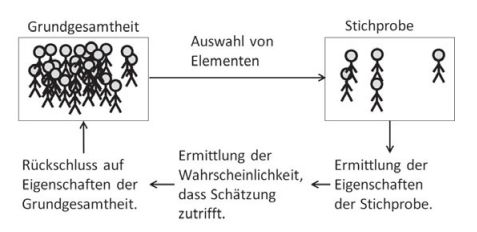
\includegraphics[width=0.80\textwidth]{images/zsmhGrundStich}
    \caption{Zusammenhang zwischen der \textit{Grundgesameheit} und \textit{Stichprobe}\protect\footnotemark}
    \label{fig:GrundgesamtheitStichprobe}
\end{figure}
\footnotetext{Vgl. Brell, \cite{Statistik von Null auf Hundert}, S. 122}

Die qualitative Forschung ist eine Methode zur Auswertung von Daten, die ausschließlich über Sprache (verbal) übermittelt
werden. Diese Methode eignet sich vor allem zur näheren Beschreibung und Analyse von subjektiven Wahrnehmungen, persönlichen
Einstellungen, Motiven und Meinungen der Befragten.\footnote{Vgl. Mayer, \cite{Interview und schriftliche Befragung}, S. 36}

Am sinnvollsten ist eine Kombination von \textit{qualitativen und quantitativen Ergebnissen}. Nach einer quantitativen
Befragung sollte eine stichprobenartige qualitative Befragung durchgeführt werden, um die Ergebnisse besser interpretieren zu können.

Unabhängig davon, ob es sich um qualitative oder quantitative Forschung handelt, sind die drei Gütekriterien \textit{Objektivität,
Zuverlässigkeit und Validität} zu erfüllen.

Sie dienen, den Forschungsprozess zu steuern und zu kontrollieren. Die Validität ist ein Maß für die Brauchbarkeit der
Methode und bezieht sich auf die tatsächliche Fähigkeit zur Messung des gewünschten Wertes. Das Ergebnis ist umso zuverlässiger,
je klarer die Fragen formuliert sind. Entscheidend für die Validität der Analyse ist die Objektivität der Messung. Dabei
ist sowohl die Durchführungsobjektivität des Befragers als auch die Auswertungs- und Interpretationsobjektivität des
Analytikers zu beachten.\footnote{Vgl. Mayer, \cite{Interview und schriftliche Befragung}, S. 54 ff., S. 88.}

Die drei Gütekriterien stehen in einem wechselseitigen Zusammenhang. Nur, wenn die Objektivität gegeben ist, kann die
Reliabilität (Zuverlässigkeit) gewährleistet werden. Ist die Reliabilität gering, kann die Validität nur mit einer gewissen Unsicherheit
vorhergesagt werden.\footnote{Vgl. Bühner, \cite{Einfuehrung in die Test- und Fragebogenkonstruktion}, S. 33 f.}

\subsection{Formulierung der Fragen}
Um eine erfolgreiche Umfrage effizient durchführen zu können, ist eine sorgfältige Vorbereitung erforderlich. Die
Erkenntnis, dass Umfragen nur bestimmte Aspekte eines Themenbereichs abdecken können, ist von entscheidender Bedeutung.
Aus diesem Grund ist eine sorgfältige und präzise Definition dieser Aspekte erforderlich. Besonderes Augenmerk ist darauf
zu richten, dass die Fragen klar formuliert sind.

Die zentrale Priorität bei der Formulierung der Fragen ist die Verständlichkeit und Eindeutigkeit. Die folgenden
Formulierungsrichtlinien sollten unbedingt beachtet werden:
\begin{itemize}
    \item Verwendung von einfachem Vokabular ohne Verwendung von Fachausdrücken, Fremdwörtern oder Ausdrücken aus anderen Sprachen.
    \item Die Fragen prägnant formulieren.
    \item Belastende Begriffe wie \textit{Ehrlichkeit} vermeiden.
    \item Hypothetische Formulierungen ausschließen.
    \item Fokussierung auf ein bestimmtes Thema für jede einzelne Frage.
    \item Vermeidung von Überforderung durch die Bereitstellung einer angemessenen Menge an Informationen pro Frage.
    \item Doppelte Verneinungen vermeiden.\footnote{Vgl. Mayer, \cite{Interview und schriftliche Befragung}, S. 89.}\\
\end{itemize}

Die genannten Kriterien sind besonders wichtig bei schriftlichen Befragungen. Um sicherzustellen, dass die Ergebnisse nicht
verfälscht werden, darf der Interviewer keine zusätzlichen Fragen stellen oder die bereits gestellten Fragen ändern.

Direkte Fragen sind geeignet, um Fakten und Wünsche zu ermitteln, während formulierte Aussagen oder Feststellungen eher
dazu dienen, die Bewertung durch die Befragten in Erfahrung zu bringen. Diese Techniken werden hauptsächlich zur Erfassung
von Einstellungen, Wahrnehmungen und Meinungen eingesetzt.

\subsection{Arten von Fragen}
In Abhängigkeit von den Anforderungen der jeweiligen Evaluation können sowohl offene als auch geschlossene Fragen gestellt werden.

Bei offenen Fragen handelt es sich um Fragen, bei denen keine Antwortmöglichkeiten vorgegeben werden. Im Anschluss an die
Frage sollte ausreichend Platz für die Beantwortung der Frage gelassen werden. Dieser Fragetyp sollte in den folgenden
Fällen verwendet werden:
\begin{itemize}
    \item Wenn die Anzahl der Antwortmöglichkeiten unbekannt ist.
    \item Wenn die Formulierung der Antwort des Auskunftspflichtigen für die Auswertung von Bedeutung ist.
    \item Wenn das Ziel der Erhebung darin besteht, die Unwissenheit und Meinung zu ermitteln.\\
\end{itemize}

Im Gegensatz zu offenen Fragen gibt es bei geschlossenen Fragen vordefinierte Antwortmöglichkeiten. Die Teilnehmerinnen
und Teilnehmer wählen ihre Antworten aus einer vorgegebenen Liste aus oder entscheiden sich zwischen den vorgegebenen
Optionen. Es gibt verschiedene Szenarien, in denen der Einsatz von geschlossenen Fragen sinnvoll ist:

\begin{itemize}
    \item Wenn die Anzahl der möglichen Antwortalternativen begrenzt und bekannt ist.
    \item Bei Umfragen, die quantitative Daten für eine statistische Auswertung erfordern.
    \item Wenn die Standardisierung der Antworten wichtig ist, um eine konsistente Analyse zu ermöglichen.\footnote{Vgl. Scholl, \cite{Die Befragung}, S. 157.}
\end{itemize}

In Bezug auf die geschlossenen Fragen ist es noch wichtig anzumerken, dass es im Wesentlichen drei Möglichkeiten für die
Benennung oder Kennzeichnung gibt:
\begin{itemize}
    \item \textbf{Numerische Benennung}: Die numerische Benennung ist ein klassisches Notationssystem mit semantischer Bedeutung. Jede Note oder Zahl ist
    eindeutig einer sprachlichen Formulierung zugeordnet. Der Abstand zwischen den einzelnen Noten ist dabei gleich groß.
    \item \textbf{Kennzeichnung durch Formen}: Eine Möglichkeit, geschlossene Fragen zu kennzeichnen, besteht darin, bestimmte Formen wie Kreise, Kästchen oder
    grafische Skalen (Symbole) zu verwenden.
    \item \textbf{Sprachliche Benennung}: Die Benennung von geschlossenen Fragen erfolgt durch klare sprachliche Ausdrücke oder Texte, welche die verschiedenen
    Antwortoptionen definieren.\footnote{Vgl. Scholl, \cite{Die Befragung}, S. 164 ff.}
\end{itemize}

\subsection{Struktur und Gliederung von Fragebögen}
Die Struktur und Gliederung eines Fragebogens spielen eine entscheidende Rolle bei der Erhebung von Daten. Ein gut
durchdachter Aufbau gewährleistet nicht nur eine klare und präzise Erfassung der benötigten Informationen, sondern
erleichtert auch die Analyse der Ergebnisse. Bei der Gestaltung eines Fragebogens sollten mehrere wichtige \textit{Schlüsselelemente}
berücksichtigt werden.

\textit{Fragetypen} sind ein zentraler Aspekt bei der Strukturierung von Fragebögen. Die geschickte Kombination von
\textit{geschlossenen} und \textit{offenen} Fragen ermöglicht es, eine umfassende Datenerhebung durchzuführen und einen
tieferen Einblick zu gewinnen.

Die \textit{Reihenfolge} der Fragen sollte einer sinnvollen \textit{Sequenz} und \textit{Logik} folgen. Der Fragebogen
sollte mit allgemeinen und weniger sensiblen Fragen beginnen, um das Vertrauen der Teilnehmer zu gewinnen. Danach sollten
spezifischere und möglicherweise persönlichere Fragen gestellt werden.

\textit{Klarheit} ist entscheidend. Klare Anweisungen, eine gut lesbare Schrift und genügend Leerraum tragen dazu bei,
Missverständnisse zu vermeiden. Sie ermutigen die Teilnehmer, präzise Antworten zu geben.

Vor dem endgültigen Einsatz des Fragebogens empfiehlt sich die Erprobung des Fragebogens im Rahmen von \textit{Pilotstudien}.
Dadurch können mögliche Probleme in Bezug auf \textit{Verständlichkeit}, \textit{Länge} und \textit{Schwierigkeitsgrad}
der Fragen identifiziert werden, bevor der endgültige Fragebogen an die Zielgruppe verteilt wird.

Die Beachtung dieser Grundsätze bei der Strukturierung und Gliederung von Fragebögen trägt dazu bei, zuverlässige und
aussagekräftige Daten für die Analyse zu gewinnen.

\subsection{Mögliche Verfälschung des Resultats}
Die Zuverlässigkeit von Umfrageergebnissen kann durch verschiedene Arten der Verfälschung beeinträchtigt werden. Zwei
häufige Verfälschungsarten sind:
\begin{itemize}
    \item \textbf{Simulation}: Teilnehmer neigen dazu, ihre Antworten absichtlich zu verfälschen, um ein bestimmtes Bild
    von sich selbst zu vermitteln. Dies kann dazu führen, dass die gegebenen Antworten nicht mit den tatsächlichen
    Meinungen oder Verhaltensweisen übereinstimmen und somit zu einer Verfälschung der Daten führen.

    \item \textbf{Dissimulation}: Es handelt sich hierbei um die bewusste Verzerrung von Informationen durch Teilnehmer
    mit dem Ziel, bestimmte Aspekte zu verschleiern oder zu verheimlichen. Diese Verzerrung kann dazu führen, dass die
    gewonnenen Daten nicht der Realität entsprechen und somit die Verlässlichkeit der Ergebnisse der Erhebung in Frage
    gestellt wird.\footnote{Vgl. Bühner, \cite{Einfuehrung in die Test und Fragebogenkonstruktion}, S. 56.}\\
\end{itemize}

Eine Vielzahl von Faktoren kann Verfälschungen auslösen. Gesellschaftliche Normen üben oft Druck auf den Einzelnen aus,
sich selbst in einem positiven Licht darzustellen, was zu einem Verhalten führen kann, das eine Simulation darstellt. Auf
der anderen Seite kann die Furcht vor sozialen Konsequenzen oder persönlichen Nachteilen dazu führen, dass Individuen
Aspekte ihrer selbst zurückhalten oder verbergen.\footnote{Vgl. Bühner, \cite{Einfuehrung in die Test und Fragebogenkonstruktion}, S. 59.}

Ein umfassendes Verständnis der Ursachen von Simulation und Dissimulation ist entscheidend für die Entwicklung wirksamer
Strategien, mit denen diese Verfälschungen in der Umfrageforschung minimiert werden können.

\subsection{Auswertung von Fragebögen}
Die Hauptintention einer Fragebogenerhebung besteht darin, eine homogene Vergleichbarkeit der individuellen Antworten der
Befragten zu gewährleisten. Dies ermöglicht eine fundierte statistische Auswertung. Eine unabdingbare Voraussetzung, um
aus den erhobenen Fragebogendaten inhaltlich sinnvolle Aussagen ableiten zu können, ist die Umrechnung der qualitativen
Antworten in quantitative Werte. Diese Umrechnung erfolgt insbesondere bei computergestützten Verfahren automatisch.

Offene Fragen erfordern eine inhaltliche Auswertung, die in der Regel in Form einer Häufigkeitsanalyse erfolgt, bei der
ähnliche Antworten zu Kategorien zusammengefasst werden. Auf diese Weise ist es möglich, die Anzahl der Befragten zu
ermitteln, die eine vergleichbare Aussage getroffen haben.

Die Auswertung geschlossener Fragen ist im Allgemeinen mit geringerem Aufwand verbunden, da die Antwortmöglichkeiten
bereits vorgegeben sind und jede einzelne Antwort zu einer dieser vorgegebenen Möglichkeiten passen muss.

Für eine angemessene grafische Darstellung der analysierten Daten sind Kreis-, Balken- und Säulendiagramme besonders
geeignet. Während Balken- und Säulendiagramme die absoluten Häufigkeiten der Antworten visualisieren und damit Unterschiede
in der Anzahl der Antworten deutlich machen, eignen sich Kreisdiagramme besonders, um relative Häufigkeiten, ausgedrückt
in Prozent, darzustellen.

\subsection{Selbst erstellter Fragebogen}
Im Verlauf dieser Diplomarbeit wurde ein Fragebogen gemäß den erläuterten Regeln und Grundlagen entwickelt. Der Fragebogen
soll am \textit{Tag der offenen Tür} an der HTBLuVA Wiener Neustadt in der Abteilung Informatik am 01.12.2024 durchgeführt
werden.

\subsubsection{Planung und Erstellung des Fragebogens}
In der Planungsphase wurde das allgemeine Layout des Fragebogens festgelegt. Anschließend wurden im Projektteam
Fragen zusammengestellt, die zur Weiterentwicklung der Applikation beitragen sollen. Der Fragebogen wurde mithilfe der
Markup-Sprache \textit{LaTeX} erstellt.

\subsubsection{Struktur und verwendete Fragetypen}
Eine klare und logische Struktur des Fragebogens sowie die Auswahl geeigneter Fragetypen spielen eine entscheidende Rolle,
um es dem Befragten zu erleichtern, die Fragen zu beantworten, und seine Motivation aufrechtzuerhalten. Der Fragebogen
beginnt mit einer kurzen Einleitung und Begrüßung, um den Befragten den Zweck des Fragebogens und den Grund für seine
Durchführung zu vermitteln.

Bei der Auswahl der Fragetypen wurde bewusst entschieden, ausschließlich geschlossene Fragen zu verwenden. Diese Entscheidung
basierte auf zwei Hauptüberlegungen. Erstens sollte die begrenzte Zeit am Tag der offenen Tür effizient genutzt werden,
und es galt, die Besucher nicht zu lange aufzuhalten. Daher wurde es als taktisch sinnvoll erachtet, keine offenen Fragen
einzubeziehen. Zweitens erleichtern geschlossene Fragen dem Projektteam die Auswertung und Interprätation der Ergebnisse.
Außerdem ermöglichte diese Entscheidung dem Projektteam, spezifische Bereiche einzugrenzen, in denen bereits bekannt war,
dass Verbesserungsbedarf besteht.

\subsubsection{Pilotstudio des Fragebogens}
Um Missverständnisse oder Unklarheiten bezüglich der gestellten Fragen zu vermeiden, wurde vor der endgültigen Durchführung
der Befragung ein Pilotversuch in einer Abschlussklasse der HTBLuVA Wiener Neustadt, Abteilung Informatik, durchgeführt.
Die Ergebnisse dieser Pilotstudie zeigten, dass die gestellten Fragen verständlich waren und ohne größere Probleme beantwortet
werden konnten.

\subsubsection{Auswertung des Fragebogens}
Um die Ergebnisse detailliert zu präsentieren, wird in diesem Abschnitt der Fragebogen verwendet, der während des
\textit{Tags der offenen Tür} der HTBLuVA Wiener Neustadt, Abteilung Informatik eingesetzt wurde. Die Fragen werden zunächst
aufgeführt, gefolgt von einer Analyse der Ergebnisse. Für diese Analyse wird das Tool \textit{Excel} verwendet, um die
Ergebnisse auszuwerten und ausführlicher darzustellen.

Diese Vorgehensweise ermöglicht es, die gesammelten Daten konkret zu veranschaulichen und deren Bedeutung für das Entwicklerteam
besser verständlich zu machen.

\begin{quote}
    Während des Tages der offenen Tür im Schuljahr 2023/2024 (25 Personen) und in einer Abschlussklasse 5CHIF 2023 / 24 (14 Personen)
    einer Schule mit Matura wurde eine Umfrage durchgeführt, um die Nutzermeinungen zur aktuellen Anwendung zu erfassen.
    Das Ziel dieser Umfrage bestand darin zu ermitteln, ob die zugrunde liegenden ausgewählten Konzepte der Informatik verstanden wurden und ob
    potenzielle Verbesserungsmöglichkeiten vorliegen.

    Anschließend wurden sieben Personen (Stichprobe) der Abschlussklasse befragt, um potenzielle Verbesserungsvorschläge
    zu ermitteln. Das Ziel dieser Umfragen bestand darin, Personen zu befragen, die bereits über grundlegendes IT-Wissen
    verfügen und dadurch besser beurteilen können, welche Aspekte verbessert werden können.
\end{quote}

Der durchgeführte Fragebogen bestand aus fünf geschlossenen Fragen, wobei bei zwei Fragen die Möglichkeit bestand, mehrere
Antworten auszuwählen. Die Fragen samt Antwortmöglichkeiten und die zugehörige Auswertung sind wie folgt:
\begin{itemize}
    \item \textbf{1. Frage}: Wie leicht war es für Sie, dass Prinzip des \textit{Nachrichtenaustauschs} zwischen zwei PCs in der Applikation zu verstehen?
    \\
    \\
    \textbf{Antwortmöglichkeiten}:\\
    Sehr schwer(5), Schwer(4), Mittel(3), Leicht(2), Sehr leicht(1)
    \\
    \begin{figure}[H]
        \centering
        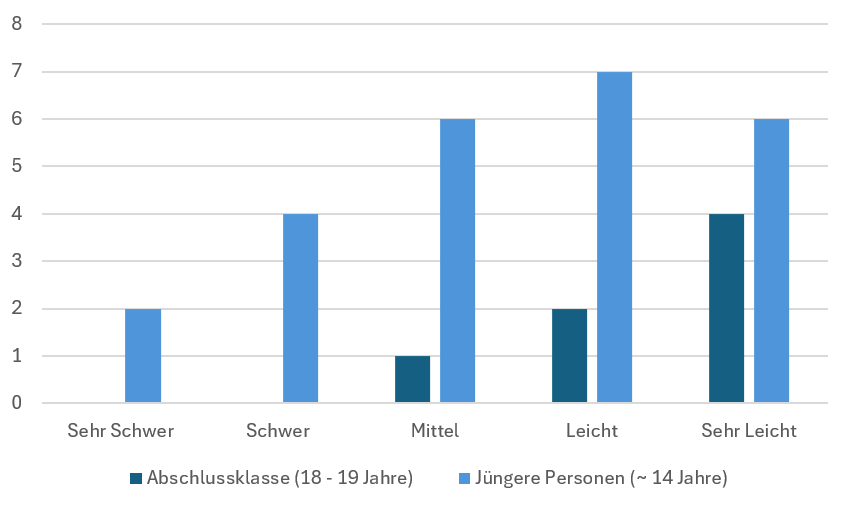
\includegraphics[width=0.9\textwidth]{images/AuswertungFrage1}
        \caption{Auswertung Frage 1}
        \label{fig:fr1}
    \end{figure}
    \item \textbf{2. Frage}: Konnten Sie das Knapsack-Problem in der Applikation ohne Probleme nachvollziehen?
    \\
    \\
    \textbf{Antwortmöglichkeiten}:\\
    Nein nicht wirklich(3), Ja mit einigen Schwierigkeiten(2), Ja problemlos(1)
    \\
    \begin{figure}[H]
        \centering
        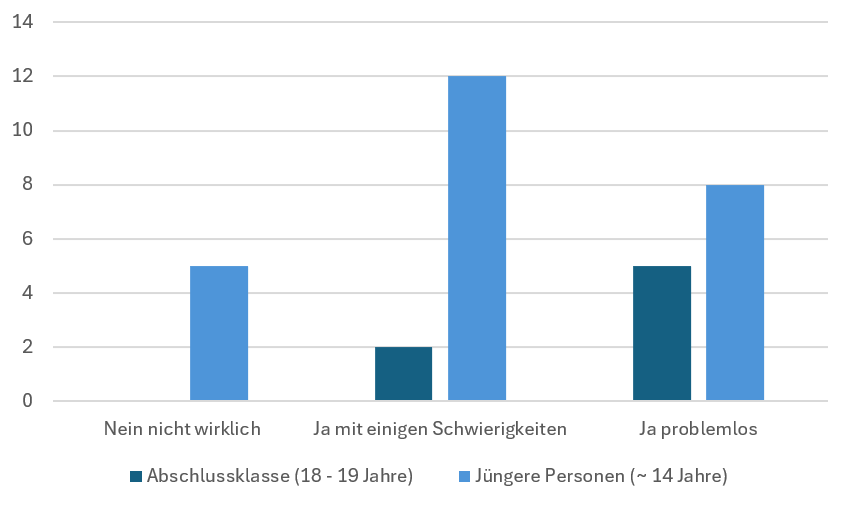
\includegraphics[width=0.9\textwidth]{images/AuswertungFrage2}
        \caption{Auswertung Frage 2}
        \label{fig:fr1}
    \end{figure}
    \item \textbf{3. Frage}: Wie sehr hat die AR-Technolgie Ihnen dabei geholfen die Informatik Prinzipien zu verstehen?
    \\
    \\
    \textbf{Antwortmöglichkeiten}:\\
    Sehr negativ(5), Negativ(4), Neutral(3), Positiv(2), Sehr positiv(1)
    \\
    \begin{figure}[H]
        \centering
        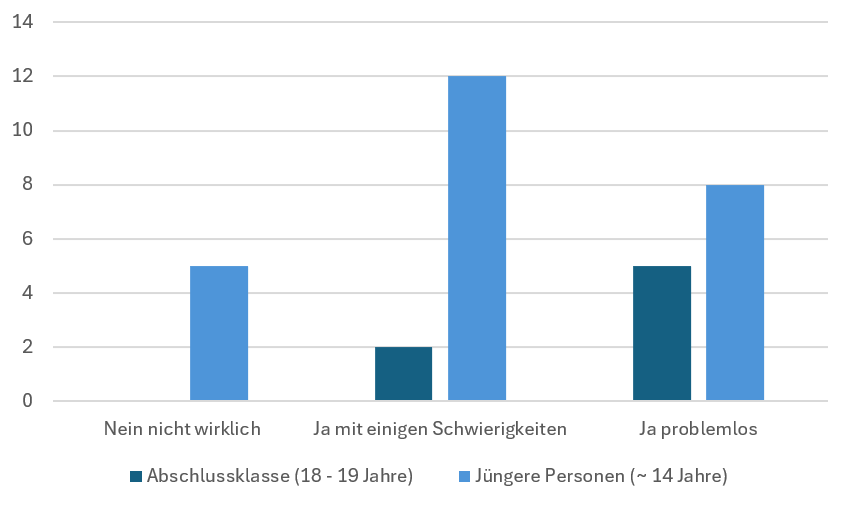
\includegraphics[width=0.9\textwidth]{images/AuswertungFrage2}
        \caption{Auswertung Frage 3}
        \label{fig:fr1}
    \end{figure}
    \item \textbf{4. Frage}: Welche der folgenden Aspekte haben Ihnen am meisten gefallen? (Mehr als eine Auswahl möglich)
    \\
    \\
    \textbf{Antwortmöglichkeiten}:\\
    Lernfördernd, Benutzerfreundlichkeit, Kreativität, Innovativ, Interaktiv
    \\
    \begin{figure}[H]
        \centering
        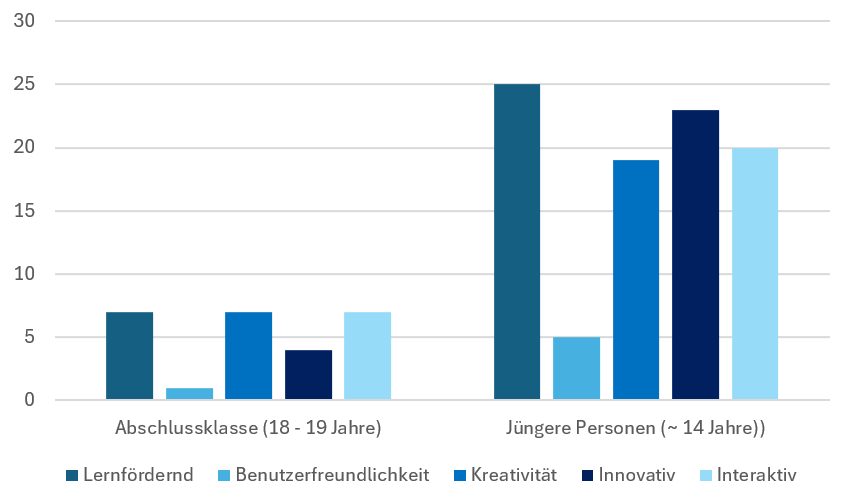
\includegraphics[width=0.9\textwidth]{images/AuswertungFrage4}
        \caption{Auswertung Frage 4}
        \label{fig:fr1}
    \end{figure}
    \item \textbf{5. Frage}: Welche der folgenden Aspekte sind noch verbesserungswürdig? (Mehr als eine Auswahl möglich
    \\
    \\
    \textbf{Antwortmöglichkeiten}:\\
    Tips / Anweisungen, Leistungsfähigkeit, Inhalt, Stabilität, Übersichtlichkeit
    \\
    \begin{figure}[H]
        \centering
        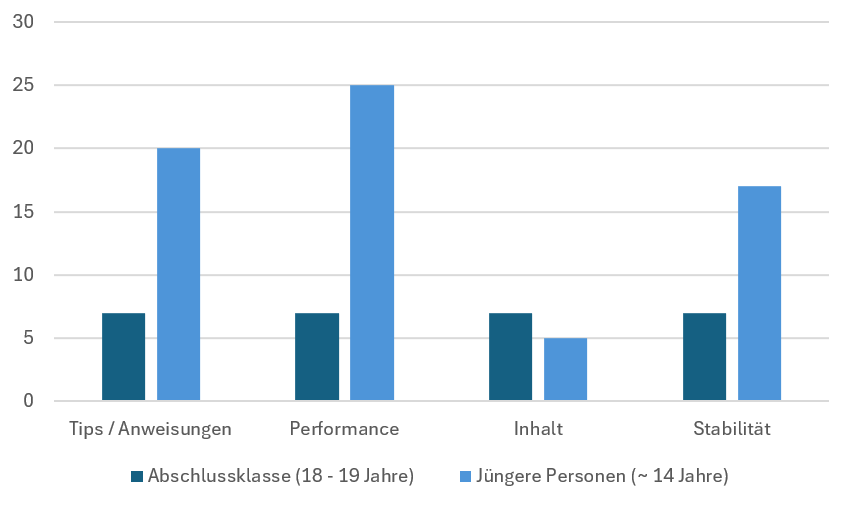
\includegraphics[width=0.9\textwidth]{images/AuswertungFrage5}
        \caption{Auswertung Frage 5}
        \label{fig:fr1}
    \end{figure}
\end{itemize}

Anhand der Auswertungen des Fragebogens wird deutlich, dass die Antworten der befragten Personen am Tag der offenen Tür
und von den Personen der Abschlussklasse stark voneinander abweichen. Dies wird besonders bei den letzten beiden Fragen,
die sich auf Aspekte, die dem Benutzer gefallen, und Verbesserungsmöglichkeiten beziehen, deutlich. Hier ist nämlich klar
zu erkennen, dass die Personen der Abschlussklasse im Vergleich zu den am Tag der offenen Tür befragten Person signifikant
mehr Angaben dazu gemacht haben. Dies lässt sich darauf zurückführen, dass sie über deutlich mehr Erfahrung im Bereich
der Entwicklung von Applikationen verfügen und generell ein vertieftes Verständnis der Informatik besitzen. Ein erfreuliches
Ergebnis ist jedoch, dass ein Großteil sowohl der am Tag der offenen Tür als auch der in der Abschlussklasse
befragten Personen die vermittelten Prinzipien der Informatik gut verstanden hat und auch, dass der Einsatz von AR-Technolgie
dabei geholfen hat diese zu verdeutlichen.

Zu erwähnen ist, dass bei der Auswertung insbesondere bei der vorletzten Frage festgestellt wurde, dass die Applikation
als nicht benutzerfreundlich bewertet wurde. Dieses Ergebnis war jedoch erwartet, da zum Zeitpunkt der Befragung das
Projekt noch in einem sehr frühen Entwicklungsstadium war und daher einige essenzielle Funktionen und Erweiterungen wie
Anweisungen und Tipps, Performance und Inhalt fehlten.

Darüber hinaus hat diese Befragung und Auswertung wichtige Ergebnisse geliefert, die dazu beigetragen haben, viele Aspekte
der Applikation maßgeblich zu erweitern und zu verbessern.
\chapter{Produktspezifikationen}
Dieses Kapitel behandelt die Planung und Spezifikation des Projekts.
Weiteres wird die verwendete Technologieauswahl begründet und mit Alternativlösungen verglichen.

\section{Eingesetzte Technologien}\marginpar{\small\(\rightarrow\) {\tiny SCHODITSCH}}
In diesem Abschnitt werden die eingsetzten Technologien näher erläutert. Zusätzlich werden Aspekte die für und gegen die
Einsetzung sprechen angeführt.

\subsection{Microsoft HoloLens2}
Zentrale Plattform des Projekts ist die Augmented-Reality-Brille "HoloLens 2" von Microsoft. Dabei handelt es sich um
eine bahnbrechende Augmented-Reality-Brille, die eine revolutionäre Verbindung zwischen der digitalen und der physischen
Welt schafft. Mit einer Reihe hochentwickelter Sensoren, Kameras und einem hochauflösenden Display eröffnet die HoloLens
2 neue Horizonte für interaktive und immersive AR-Erlebnisse.

Die HoloLens 2 bietet eine beeindruckende Immersion, die es dem Nutzer ermöglicht, digitale Objekte nahtlos in seine
Umgebung zu integrieren. Dank des fortschrittlichen Hand- und Blickverfolgungssystems können Benutzer mit den holografischen
Elementen interagieren, als wären sie Teil ihrer realen Welt. Dies ermöglicht eine breite Palette von Anwendungen, von
Unterhaltung über Bildung bis hin zu industriellen Anwendungen.

\subsection{Kriterien}
Bei der Auswahl der Technologien, die für die Entwicklung der geplanten Anwendung eingesetzt werden, war es besonders
wichtig, dass diese über eine gute Dokumentation und eine große Entwicklergemeinschaft verfügen, falls Fragen auftauchen,
für die nicht direkt im Internet eine Lösung gefunden werden kann. Außerdem sollten sie einfach zu bedienen sein und vor
allem eine performante Nutzung der Anwendung gewährleisten.

\subsection{Game Engine}
Um einen reibungslosen Verlauf des Projekts zu gewährleisten, ist die sorgfältige Auswahl der richtigen \textit{Game Engine} von
entscheidender Bedeutung. Die Game Engine fungiert als fundamentale Plattform für die Entwicklung und Erstellung von
Videospielen, indem sie eine umfassende Palette von Werkzeugen, Bibliotheken und Funktionen bereitstellt, die Entwicklern
hilft, Spiele zu konzipieren, umzusetzen und zu optimieren. In diesem Abschnitt werden zwei potenzielle Game Engines,
die für das Projekt in Betracht gezogen wurden, eingehend untersucht und anschließend die Gründe für die getroffene Auswahl
erläutert.

\subsubsection{Unity}
Unity ist eine Game Engine, die von Entwicklern weltweit für die Erstellung von 2D- und 3D-Spielen genutzt wird. Sie
unterstützt verschiedene Plattformen wie PC, Konsolen, Mobilgeräte und AR/VR-Geräte\footnote{Unity.com \cite{Plattformen}}. Unity bietet Entwicklern eine
umfangreiche Sammlung von Werkzeugen und Ressourcen, um Spiele schnell zu prototypen und zu entwickeln.

Ein herausragendes Merkmal von Unity ist der Asset Store. Hier können Entwickler Assets wie 3D-Modelle, Texturen, Sounds
und Plugins kaufen oder verkaufen. Dadurch können sie ihre Projekte mit hochwertigen Inhalten erweitern und verbessern,
ohne alles von Grund auf neu erstellen zu müssen.\footnote{Assetstore.Unity.com \cite{Unity Asset Store}} Unity bietet außerdem eine starke Community-Unterstützung mit Foren,
Tutorials und Schulungen, was besonders für neue Entwickler hilfreich ist.

Die Programmierung in Unity erfolgt hauptsächlich durch die Verwendung von C-Sharp. Diese ist sowohl für
erfahrene Entwickler als auch für Anfänger zugänglich. Unity ist aufgrund der Kombination von benutzerfreundlichen Werkzeugen,
einer großen Community und einer breiten Plattformunterstützung eine beliebte Wahl für Indie-Entwickler sowie für große Studios.

\subsubsection{Unreal Engine}
Die Unreal Engine ist eine leistungsstarke Game Engine, die für ihre hochwertigen Grafiken und fortgeschrittenen Funktionen
bekannt ist. Sie wird häufig für die Entwicklung von AAA-Titeln sowie für hochwertige VR-Erfahrungen verwendet. Die Engine
bietet branchenführende Grafikfunktionen wie fortschrittliche Beleuchtung, Partikelsysteme, Physiksimulationen und Echtzeit-Rendering.

Eine bemerkenswerte Funktion der Unreal Engine ist das Blueprints-System (siehe folgender Absatz). Es ermöglicht Entwicklern, Spiele und interaktive
Inhalte ohne herkömmlichen Programmiercode zu erstellen. Dadurch wird die Engine besonders zugänglich für Künstler und
Designer, die möglicherweise keine tiefen Programmierkenntnisse haben.

Die Unreal Engine bietet eine umfangreiche Sammlung von vorgefertigten Assets und Werkzeugen sowie einen integrierten
Marketplace, auf dem Entwickler zusätzliche Inhalte erwerben können. Sie unterstützt eine Vielzahl von Plattformen,
darunter PC, Konsolen, Mobilgeräte und VR-Headsets.

Insgesamt ist die Unreal Engine eine leistungsstarke Wahl für Entwickler, die hochwertige Grafiken und fortschrittliche
Funktionen in ihren Spielen und Anwendungen benötigen. Sie wird häufig von größeren Studios genutzt, die Zugang zu hochwertigen
Tools und Support benötigen.\footnote{Unrealengine.com \cite{Wir liefern die Engine. Sie machen sie Unreal}}

\subsubsection*{Blueprint Visual Scripting}
Das Blueprint Scripting System ist eine leistungsstarke visuelle Programmierumgebung innerhalb der Unreal Engine. Es
ermöglicht Entwicklern, komplexe Logik und Interaktionen ohne traditionelle Programmierkenntnisse zu erstellen. Das System
basiert auf dem Konzept von \textit{Blueprints}, die visuelle Darstellungen von Logik und Funktionen sind.

Die Verwendung von Blueprints bietet eine Reihe von Vorteilen. Einerseits ermöglicht es Künstlern und Designern ohne
tiefgreifende Programmiererfahrung, komplexe Interaktionen und Spielmechaniken zu implementieren. Durch das Drag-and-Drop-Interface
können Benutzer Funktionsblöcke miteinander verbinden und so den Fluss der Spiellogik steuern.

Andererseits erleichtert das Blueprint-System die Iteration und Prototypisierung. Da Änderungen visuell vorgenommen
werden können, können Entwickler schnell experimentieren und Anpassungen vornehmen, um das gewünschte Verhalten zu erreichen.
Dies beschleunigt den Entwicklungsprozess und ermöglicht es Teams, flexibel auf Feedback und sich ändernde Anforderungen zu reagieren.

Das Blueprint Scripting System bietet zudem eine hohe Flexibilität und Erweiterbarkeit. Entwickler können benutzerdefinierte
Blueprints erstellen und sie in anderen Projekten wiederverwenden, was die Effizienz erhöht und die Entwicklung
beschleunigt.\footnote{Unreal Engine Dokumentation \cite{Blueprints Visual Scripting}}

\subsubsection{Game Engine Auswahl und Wechsel im Projektverlauf}
Bei Projektbeginn wurde nach umfassender Recherche und Evaluierung verschiedener Optionen entschieden, die Unreal Engine
als primäre Entwicklungsumgebung für dieses Projekt zu verwenden. Diese Entscheidung wurde aufgrund mehrerer überzeugender
Faktoren getroffen, darunter insbesondere das beliebte Blueprint Visual Scripting, das die Entwicklung von interaktiven
Inhalten erleichtert und auch für Personen ohne umfangreiche Programmierkenntnisse zugänglich macht. Zusätzlich zu diesem
herausragenden Merkmal wurden weitere Aspekte berücksichtigt, die die Unreal Engine zu einer attraktiven Wahl machten,
wie beispielsweise ihre leistungsstarken Grafikfunktionen, die branchenweit anerkannt sind, sowie ihre Unterstützung für
die Entwicklung hochwertiger VR-Erfahrungen und AAA-Titel.

\subsubsection*{Herausforderungen im ersten Monat des Entwicklungsprozesses}
Trotz der zu Beginn getroffenen Entscheidung für die Unreal Engine traten im Verlauf des ersten Monats des Entwicklungsprozesses
bestimmte Herausforderungen auf. Diese Herausforderungen können als unerwartete Schwierigkeiten betrachtet werden, die während
der Umsetzung des Projekts auftraten und zweifel an der ursprünglichen Entscheidung mit sich brachte.
Im Einzelnen wurden folgende Herausforderungen identifiziert:
\begin{enumerate}
    \item \textbf{Mangelhafte Dokumentation für AR-Entwicklung in der Unreal Engine:} Die unzureichende Dokumentation
    für die Entwicklung von Augmented Reality (AR)-Anwendungen in der Unreal Engine erwies sich als erhebliche Hürde.
    Fehlende detaillierte Anleitungen und Referenzen für AR-spezifische Funktionen behinderten die effiziente Integration von AR-Elementen.
    \item \textbf{Begrenzte Verfügbarkeit von AR-spezifischen Online-Tutorials:} Ein Mangel an Online-Tutorials,
    die sich speziell mit der Entwicklung von AR-Anwendungen in der Unreal Engine befassten, führte zu einer
    beträchtlichen Lernkurve für das Entwicklerteam und verzögerte den Implementierungsprozess von AR-spezifischen Features.
    \item \textbf{Komplexität der AR-Entwicklung in der Unreal Engine:} Die Unreal Engine erwies sich als sehr
    anspruchsvoller für Neueinsteiger in Bezug auf die Umsetzung von AR-spezifischen Funktionen. Die Notwendigkeit, komplexe Skripte zu
    erstellen und vielfältige Einstellungen anzupassen, führte zu einem erhöhten Zeitaufwand für die Umsetzung von AR-Elementen.
    \item \textbf{Eingeschränkte Community-Unterstützung für AR-Entwicklung:} Im Vergleich zu Unity war die Community-Unterstützung
    für die AR-Entwicklung in der Unreal Engine begrenzt. Die Verfügbarkeit von Ratschlägen und Lösungen für spezifische
    AR-Herausforderungen war eingeschränkt, was die Eigenständigkeit bei der Lösung von Problemen beeinträchtigte.
\end{enumerate}

Diese Herausforderungen bildeten die Grundlage für die strategische Entscheidung des Projektteams, von Unreal Engine
zu Unity zu wechseln. Der Wechsel ermöglichte eine effizientere und zielführende Entwicklung der AR-Applikation,
gestützt durch Unity's umfassende Unterstützung, detaillierte Dokumentation und breite Community-Ressourcen.

\subsection{Unity foundation packages}
Um Augmented Reality (AR)-Applikationen in Unity erfolgreich zu entwickeln, sind bestimmte \textit{Foundation Packages}
erforderlich. Diese Pakete müssen in Unity importiert werden, um grundlegende Funktionalitäten bereitzustellen, die für
die erfolgreiche Umsetzung einer AR-Applikation notwendig sind. Im Folgenden werden die beiden wesentlichen Pakete näher
erläutert, die für die Funktionalität einer solchen Applikation unerlässlich sind.

\subsubsection{MRTK3}
Das Mixed Reality Toolkit 3 (MRTK3), welches Sowohl für Unity als auch in der Unreal Engine anwendbar ist, ist ein leistungsstarkes Open-Source-Entwicklungstoolkit, das von Microsoft entwickelt
und gepflegt wird. Es ist speziell darauf ausgerichtet, die Entwicklung von Mixed-Reality-Anwendungen zu erleichtern,
indem es eine umfassende Sammlung von Komponenten, Skripten und Assets bereitstellt. MRTK3 bietet Entwicklern eine Vielzahl
von Funktionen und Werkzeugen, die speziell für die Erstellung von Anwendungen für Augmented Reality (AR), Virtual Reality
(VR) und Mixed Reality (MR) optimiert sind.

Das Toolkit umfasst eine breite Palette von Funktionen, darunter Interaktionselemente wie Hand- und Gestenerfassung,
räumliches Mapping, Physiksimulationen für Objekte in der realen Welt, Benutzerschnittstellen-Design-Werkzeuge und vieles
mehr. MRTK3 ist plattformübergreifend und unterstützt verschiedene AR-/VR-Headsets sowie andere Mixed-Reality-Geräte.

Die Bedeutung von MRTK3 für die Entwicklung von AR-Applikationen liegt in seiner Fähigkeit, Entwicklern eine solide
Grundlage und eine Vielzahl von vordefinierten Komponenten und Tools zu bieten, die den Entwicklungsprozess beschleunigen
und vereinfachen. Durch die Verwendung von MRTK3 können Entwickler komplexe AR-Anwendungen schneller prototypisieren und
implementieren, da sie auf eine umfangreiche Bibliothek von Funktionen zugreifen können, die speziell für AR-Szenarien
optimiert sind. Dies erhöht die Effizienz der Entwicklung und ermöglicht es den Entwicklern, sich auf die Gestaltung und
Umsetzung innovativer AR-Erfahrungen zu konzentrieren, ohne sich um die Grundlagen der AR-Entwicklung kümmern zu müssen.\footnote{Microsoft-Dokumentation \cite{Mixed Reality Toolkit 3}}

\subsubsection{\label{sec:openxr}Microsoft OpenXR Plugin}
Das Microsoft OpenXR Plugin stellt eine bedeutende Komponente im Kontext der Entwicklung von Augmented Reality (AR)-Applikationen
innerhalb der Entwicklungsumgebung dar. Entwickelt und bereitgestellt von Microsoft, ermöglicht dieses Plugin die
nahtlose Integration des OpenXR-Standards in Unity. OpenXR, initiiert durch die Khronos Group, fungiert als branchenweiter
Standard zur Vereinheitlichung der XR-Anwendungsentwicklung, wobei XR für Extended Reality steht und sowohl Augmented
Reality (AR), Virtual Reality (VR) als auch Mixed Reality (MR) umfasst.

Das Microsoft OpenXR Plugin erleichtert Entwicklern die Arbeit innerhalb von Unity, indem es eine reibungslose Integration
des OpenXR-Standards ermöglicht. Hierdurch erhalten Entwickler Zugang zu einer breiten Palette von Funktionen und
Möglichkeiten, die durch den OpenXR-Standard standardisiert sind, inklusive plattformübergreifender Kompatibilität sowie
optimierter Leistung für XR-Anwendungen.

Die Relevanz des Microsoft OpenXR Plugins für die AR-Entwicklung liegt in seiner Fähigkeit, eine konsistente Entwicklungsumgebung
für XR-Anwendungen innerhalb von Unity zu schaffen. Durch die Nutzung dieses Plugins können AR-Entwickler die Vorteile
des OpenXR-Standards voll ausschöpfen, einschließlich verbesserte Kompatibilität, Leistung und Zukunftssicherheit ihrer Anwendungen.

Zusätzlich erlaubt das Plugin den Entwicklern den Zugriff auf spezifische Funktionen und Optimierungen, die von Microsoft
speziell für die AR-Entwicklung entwickelt wurden. Dies beinhaltet beispielsweise Features zur Verbesserung der
AR-Umgebungserkennung, Handhabung von Eingaben sowie Optimierung der Grafikleistung für AR-Anwendungen.\footnote{Khronos Group \cite{OpenXR Plugin}}

\subsubsection{Integrationsprozess der Plugins}
Zur Integration der genannten Plugins in
den Unity Editor, um diese verwenden zu können, wird das externe Tool namens \textit{Mixed Reality Feature Tool} von Microsoft verwendet. Dieses Tool
fungiert als umfassende Sammlung von Plugins und Erweiterungen im Bereich der Augmented und Virtual Reality Entwicklung
für Unity. Neben den erwähnten Plugins umfasst es weitere wichtige Erweiterungen, darunter:
\begin{itemize}
    \item Azure Mixed Reality Services
    \item Experimental
    \item Mixed Reality Toolkit
    \item Plattform Support
    \item Spatial Audio
    \item World Locking Tools
    \item Weitere Funktionen (Other features)
\end{itemize}

Um die Integration durchzuführen, müssen innerhalb des \textit{Plattform Support} Bereichs des \textit{Mixed Reality Feature Tools}
sowohl das \textit{Mixed Reality OpenXR Plugin} als auch das gesamte MRTK3-Paket ausgewählt werden. Nach der Auswahl
dieser Pakete ist es erforderlich, sie zu validieren und anschließend in das Unity-Projekt zu importieren.

Dieser Prozess gewährleistet eine erfolgreiche Integration der benötigten Plugins und Erweiterungen, die für die Entwicklung
von Augmented Reality-Anwendungen in Unity von entscheidender Bedeutung sind.

\subsection{Wahl des Modellierungsprogramm} \label{sec:wahlblender} \marginpar{\small\(\rightarrow\) {\tiny LAMPEL}}
Durch Unity und die Open-Source-lastige Modellierungscommunity gibt es verschiedene Möglichkeiten, um an die 3D-Modelle
zu gelangen, die für die Anwendung der Szenarien benötigt werden.

Eine Möglichkeit besteht darin, auf weit verbreitete 3D-Modelle auf sogenannten \textit{Asset Stores} zurückzugreifen,
wie zum Beispiel dem von Unity selbst. Dort können sie entweder gekauft oder kostenlos heruntergeladen werden. Die
verschiedenen Angebote unterscheiden sich in der Texturqualität und dem Modellierungsaufwand.
\footnote{Unity \cite{Asset Store}}

Eine weitere Möglichkeit besteht darin, die Modelle selbst in einem Modellierungsprogramm zu entwerfen. Diese Variante
ist zwar zeitintensiver und aufwendiger, führt jedoch zu maßgeschneiderten Modellen, die den Wünschen und Anforderungen
des Projekts entsprechen. Es gibt verschiedene Programme, die die Anforderungen erfüllen würden. Beispielsweise würden
Blender \footnote{Blender \cite{Blender Allgemein}}, 3ds Max \footnote{Autodesk \cite{3DS Max}} von Autodesk oder
Cinema 4D \footnote{Maxon \cite{Cinema 4D}} von Maxon in Frage kommen. Diese Programme unterscheiden sich nur hinsichtlich
der Bedienung, aber der eigentliche Zweck ist gleich.

Nach Absprachen innerhalb des Teams wurde beschlossen, das Modellierungsprogramm Blender zu benutzen, da eines der
Teammitglieder bereits gewisses Wissen in der Bedienung und Modellierung mit diesem Programm angehäuft hat. Nicht nur
das war der ausschlaggebende Punkt, sondern auch die große Benutzergemeinschaft in Blender mit zahlreichen Tutorials
und Hilfestellungen für auftretende Herausforderungen.

Obwohl diese Variante einen höheren Zeitaufwand und zusätzliche Komplexität des Projekts mit sich bringt, erhält man
am Ende eine Sammlung von Objekten, die vollständig den Anforderungen und Wünschen entspricht. Zudem ist dies die
kostengünstigste Methode, da der Kauf von Modellen oder einer kostenpflichtigen Modellierungsplattform vermieden werden
konnte, um hohe Kosten zu vermeiden.

\subsubsection{Wie funktioniert Blender im Allgemeinen?}
Die Applikation Blender ist sehr komplex. Daher werden in der folgenden Beschreibung nur die Schlüsselaspekte und die
Funktionalität von Blender für unseren speziellen Anwendungsbereich hervorgehoben.

\begin{itemize}
    \item \textbf{Benutzeroberfläche und Interaktion}\\
    Die Benutzeroberfläche von Blender ist hoch anpassbar, obwohl sie komplex gestaltet ist. Sie enthält 3D-Modelle,
    Ansichten, Fenster und Panels. Benutzer interagieren mit Objekten und Werkzeugen über Maus- und Tastaturbefehle.
    Die Effizienz der Arbeit und die Modellierungsdauer hängen stark von der Erfahrung des Benutzers ab, insbesondere
    von der Nutzung von Shortcuts und Hotkeys.\footnote{Blender \cite{Benutzeroberfläche}}

    \item \textbf{3D-Modellierung}\\
    Blender ermöglicht die Erstellung von 3D-Modellen durch die Verwendung von Primitiven wie Würfeln, Kugeln,
    Flächen und Kurven. Diese können bearbeitet und modifiziert werden, um komplexe Formen zu erstellen.
    Modellierungswerkzeuge wie Extrusion, Verschiebung, Skalierung und Rotation stehen zur Verfügung.
    \footnote{Blender \cite{Toolbar}}

    \item \textbf{Materialien und Texturen}\\
    Um realistische Oberflächen zu erzeugen, können Materialien erstellt und Texturen auf Objekte angewendet werden.
    Blender ermöglicht die Feinanpassung von Materialeigenschaften wie Diffusreflexion, Glanz, Transparenz und Emission.
    \footnote{Blender \cite{Materials}}

    \item \textbf{Gemeinschaft und Ressourcen}\\
    Blender hat eine engagierte Benutzergemeinschaft, die umfassende Dokumentation, Tutorials und Foren
    bereitstellt. Diese Ressourcen erleichtern die Einarbeitung und Problemlösung.
\end{itemize}

Blender wird im gesamten Projekt eingesetzt, angefangen beim Entwurf und der Erstellung des Hauptmenüs bis hin zur
Gestaltung jedes einzelnen Objekts. Es wird hauptsächlich für die digitale Modellierung der wichtigsten täglichen
Gegenstände von Schülern verwendet. Das Ziel besteht darin, am Ende eine umfangreiche Sammlung von Objekten zu haben,
um den Benutzern eine vielfältige und zahlreiche Auswahl an verschiedenen Modellen zu bieten.

% Define colors
\definecolor{keywordcolor}{RGB}{255,0,0}
\definecolor{Classcolor}{RGB}{90, 90, 90}
\definecolor{Funcolor}{RGB}{191, 64, 191}
\definecolor{Logiccolor}{RGB}{51, 179, 255}
\definecolor{commentcolor}{RGB}{0,128,0}
\definecolor{stringcolor}{RGB}{163,21,21}

% Language definition
\lstdefinelanguage{CS}{
    language=C,
    morekeywords=
        {using, public, private, class, yield, return, new, if, else, out, try, catch, for, while, throw, foreach, in, using},
    morekeywords=[2]
        {ARRaycastManager, ARPlaneManager, GameObject, InventoryController, Vector3, ARPlane, Ray, RaycastHit, GetComponent, MeshRenderer, Quaternion},
    morekeywords=[3]
        {Start, Update, Awake, DelayedStart, IsPointerOverPlane, GetCurrentPlaneUnderGaze, SetPlaneColor, PlaceObjectOnDesk, ScreenPointToRay, SetActive, Euler, SetInventoryObject, Raycast},
    morekeywords=[4]
        {+, -, /, *, !, =, 0, 1, 2, 3, 4, 5, 6, 7, 8, 9, null, true, false}, % Define symbols as keywords
    morecomment=[l]{//},
    morecomment=[s]{/*}{*/},
    morestring=[b]",
    sensitive=true
}

\lstdefinelanguage{JavaScript}{
    morekeywords={async, await, break, case, catch, class, const, continue, debugger, default, delete, do, else, export, extends, finally, for, function, if, import, in, instanceof, let, new, return, super, switch, this, throw, try, typeof, var, void, while, with, yield},
    morecomment=[l]{//},
    morecomment=[s]{/*}{*/},
    morestring=[b]',
    morestring=[b]"
}

% Listings settings
\lstset{
    language=CS,
    basicstyle=\footnotesize\ttfamily,
    keywordstyle=\color{keywordcolor}\bfseries,
    keywordstyle=[2]\color{Classcolor},
    keywordstyle=[3]\color{Funcolor},
    keywordstyle=[4]\color{Logiccolor},
    commentstyle=\color{commentcolor},
    stringstyle=\color{stringcolor},
    showstringspaces=false,
    breaklines=true,
    frame=single,
    numbers=left,
    numberstyle=\tiny\color{gray},
    tabsize=4,
    captionpos=b
}

\chapter{Feinkonzept und Realisierung}

\section{Entwicklungsumgebungen}
\subsection{Visual Studio 2022}
Visual Studio 2022 ist eine integrierte Entwicklungsumgebung (IDE) von Microsoft, die speziell für die Entwicklung von
Softwareanwendungen, Webanwendungen und Desktop-Anwendungen konzipiert ist. Es handelt sich um eine umfangreiche
Entwicklungsumgebung, die von Entwicklern weltweit für eine breite Palette von Anwendungsfällen eingesetzt wird.

\subsection{Unity}
Der Unity-Editor, entwickelt von Unity Technologies, fungiert als umfassende integrierte Entwicklungsumgebung (IDE)
und zentrale Arbeitsumgebung für die Konzeption und Umsetzung von 2D-, 3D-, Augmented Reality (AR) und Virtual Reality
(VR) Anwendungen und Spielen. Als Kernelement der Unity-Plattform spielt der Editor eine entscheidende Rolle in der
Entwicklung von Projekten, die auf Unity-Technologien basieren.

Die Funktionalität des Unity-Editors erstreckt sich über verschiedene Aspekte der Softwareentwicklung, angefangen bei
der visuellen Gestaltung von Szenen und Spielwelten bis hin zur Implementierung komplexer Logik und Interaktionen. Die
folgenden Abschnitte vertiefen die Schlüsselmerkmale und Funktionen des Unity-Editors, die ihn zu einem essenziellen
Werkzeug für Entwickler machen.

\subsubsection{Multidisziplinäre Unterstützung und Integration}
Der Unity-Editor zeichnet sich durch seine multidisziplinäre Unterstützung aus, die Entwicklern ermöglicht, kollaborativ
an Projekten zu arbeiten. Künstler, Entwickler und Designer können innerhalb derselben Umgebung zusammenarbeiten,
wodurch ein nahtloser Austausch von Assets, Szenen und Ressourcen ermöglicht wird. Die Integration von Grafik-,
Physik- und Audio-Engines erleichtert die Schaffung immersiver und ansprechender digitaler Umgebungen.

\subsubsection{Szenengestaltung und Asset-Management}
Ein zentrales Merkmal des Unity-Editors ist die intuitive Szenengestaltung, die es Entwicklern ermöglicht,
2D- und 3D-Szenen durch Drag-and-Drop-Operationen zu erstellen und anzupassen. Das Asset-Management ermöglicht eine
effiziente Organisation von Ressourcen wie Modelle, Texturen und Audio-Dateien. Hierbei kommt dem Editor eine
Schlüsselrolle in der Strukturierung und Verwaltung umfangreicher Projekte zu.

\subsubsection{Programmierung und Skripterstellung}
Der Unity-Editor integriert leistungsstarke Programmierfunktionen, die Entwicklern erlauben, Skripte in C-Sharp oder
JavaScript zu verfassen. Die Implementierung von Logik, Interaktionen und Funktionalitäten erfolgt durch die
Integration von Skripten in GameObjects und Szenen. Die Echtzeitansicht von Codeänderungen unterstützt einen
iterativen Entwicklungsprozess.

\subsubsection{Unterstützung für Augmented Reality (AR) und Virtual Reality (VR)}
Der Unity-Editor ist essenziell für die Entwicklung von AR- und VR-Anwendungen. Durch die Integration von AR Foundation
und XR Interaction Toolkit bietet der Editor leistungsstarke Werkzeuge zur Erstellung immersiver Erlebnisse. Die
Möglichkeit, Szenen in Echtzeit in AR- und VR-Geräten zu überprüfen, unterstützt Entwickler bei der Feinabstimmung
und Optimierung ihrer Projekte.

\subsubsection{Erweiterte Debugging- und Profiling-Werkzeuge}
Der Unity-Editor stellt umfassende Debugging- und Profiling-Werkzeuge zur Verfügung, um die Leistung und Funktionalität
von Anwendungen zu optimieren. Durch Echtzeit-Inspektion, Fehlerverfolgung und Ressourcenüberwachung unterstützt der
Editor Entwickler bei der Identifizierung und Behebung von Problemen, um eine reibungslose Ausführung der Anwendungen
sicherzustellen.

\subsubsection{Aufbau einer Unity-Applikation}
Die Struktur einer Unity-Applikation ist entscheidend für eine effektive Entwicklung und Organisation von 3D-Anwendungen
und Spielen. Eine typische Unity-Anwendung besteht aus verschiedenen Schlüsselelementen, darunter Szenen, GameObjects,
Komponenten, Skripte und Assets. Diese werden koordiniert durch die Hauptkomponente der Anwendung, die sogenannte
"GameManager" oder "MainScene". In diesem Abschnitt werden die grundlegenden Bausteine einer Unity-Anwendung sowie
bewährte Praktiken für die Strukturierung und Verwaltung dieser Elemente beleuchtet.

\subsubsection{Lebenszyklusmethoden in Unity}
Die Entwicklung von Augmented Reality (AR)-Applikationen in Unity erfordert ein tiefgreifendes Verständnis der
Lebenszyklusmethoden, die in MonoBehaviour-Klassen implementiert werden können. Diese Methoden regeln den Fluss der
Programmlogik und ermöglichen Entwicklern, spezifische Aktionen zu bestimmten Zeitpunkten im Lebenszyklus einer
Anwendung auszuführen.

\begin{itemize}
    \item \textbf{Awake():} Die \texttt{Awake()}-Methode wird aufgerufen, wenn das Skript erstellt wird. Dies geschieht
    vor anderen Initialisierungsmethoden wie \texttt{Start()}. Sie eignet sich für die Durchführung von
    Initialisierungen, bei denen auf andere Skriptkomponenten oder Ressourcen zugegriffen werden soll. Der Hauptzweck
    besteht darin, die Ressourcen für das Skript vorzubereiten.
    \item \textbf{Start():} Die \texttt{Start()}-Methode wird vor dem ersten Frame aufgerufen und bietet die
    Möglichkeit, Initialisierungsaufgaben durchzuführen. Im Gegensatz zu \texttt{Awake()} garantiert \texttt{Start()}
    die vollständige Initialisierung aller GameObjects in der Szene. Entwickler nutzen diese Methode oft für
    Konfigurationen und Vorbereitungen, die spezifisch für die Startphase der Anwendung sind.
    \item \textbf{Update():} Die \texttt{Update()}-Methode ist von entscheidender Bedeutung, da sie in jedem Frame
    aufgerufen wird. Hier kann kontinuierliche Logik ausgeführt werden, wie etwa die Aktualisierung von Animationen,
    die Verarbeitung von Benutzereingaben oder die Anpassung von Positionen basierend auf der Zeit. Es ist wichtig zu
    beachten, dass \texttt{Update()} häufig aufgerufen wird und daher effizient implementiert werden sollte.
    \item \textbf{LateUpdate():} Ähnlich wie \texttt{Update()}, wird aber nachdem alle \texttt{Update()}-Methoden
    aufgerufen wurden. Dies ist besonders nützlich, wenn Anpassungen oder Berechnungen vorgenommen werden müssen,
    nachdem andere GameObjects und Skripte bereits ihre \texttt{Update()}-Logik abgeschlossen haben. Beispielsweise
    eignet sich \texttt{LateUpdate()} gut für Kamera-Anpassungen, bei denen die Position anderer GameObjects bereits
    aktualisiert wurde.
    \item \textbf{OnEnable() und OnDisable():} Die \texttt{OnEnable()}-Methode wird aufgerufen, wenn ein Skript
    aktiviert wird, während \texttt{OnDisable()} aufgerufen wird, wenn es deaktiviert wird. Diese Methoden bieten
    die Möglichkeit, spezifische Aktionen auszuführen, wenn ein Skript seine Ausführung aufnimmt oder beendet.
    Entwickler können diese nutzen, um Ressourcen zu laden oder freizugeben, Abonnements auf Ereignisse
    einzurichten oder abzubrechen, oder um andere vorbereitende oder aufräumende Maßnahmen durchzuführen.
\end{itemize}

\subsubsection{Unity Szenen}
Unity-Szenen bilden das grundlegende Gerüst für die Gestaltung von Inhalten in der Unity-Entwicklungsumgebung. Sie stellen
Assets dar, die alle oder einen Teil eines Spiels oder einer Anwendung enthalten. Szenen bieten eine strukturierte Möglichkeit,
verschiedene Elemente wie \textit{Umgebungen}, \textit{Charaktere}, \textit{Hindernisse}, \textit{Dekorationen} und
\textit{Benutzeroberflächen} zu organisieren und miteinander zu verknüpfen.

Ein wichtiger Aspekt von Unity-Szenen ist ihre Flexibilität. In einem Projekt können \textit{beliebig viele} Szenen erstellt werden,
um die Organisation und Entwicklung des Spiels zu erleichtern. Durch das modulare Konzept von Szenen können Entwickler
einzelne Teile des Spiels separat \textit{bearbeiten} und \textit{optimieren}, was die Zusammenarbeit im Team und die
Wartung des Projekts vereinfacht.

Unity-Szenen dienen nicht nur der Darstellung von Inhalten, sondern auch der \textit{Steuerung} des Spielablaufs. Durch die gezielte
Aktivierung und Deaktivierung von Szenen können verschiedene Abschnitte des Spiels geladen und entladen werden, was die
Leistung und Ressourcennutzung optimiert.

Insgesamt bieten Unity-Szenen eine leistungsstarke und flexible Möglichkeit, Spiele und Anwendungen zu \textit{strukturieren}, zu
\textit{organisieren} und zu \textit{verwalten}. Sie bilden das Grundgerüst für die Entwicklung von Inhalten in Unity und ermöglichen es
Entwicklern, ihre Visionen zu verwirklichen und ansprechende Spielerlebnisse zu schaffen.\footnote{Unity Dokumentation \cite{Scenes}}

\subsubsection{Unity Manager}
Die präzise und immersive Umsetzung von Augmented-Reality-(AR-)Applikationen erfordert den Einsatz spezialisierter Manager,
die grundlegende Funktionen bereitstellen, die für die erfolgreiche Umsetzung verschiedener Szenarien unerlässlich sind.
In dieser Applikation werden zwei Manager aus der breiten Palette von Unity bereitgestellten Managern verwendet. Diese
sind die folgenden:
\begin{itemize}
    \item \textbf{ARPlaneManager\footnote{Unity Dokumentation\cite{PlaneManager}}:}
    Der ARPlaneManager ist ein bedeutender Bestandteil von Unity's Augmented Reality (AR)-Entwicklungsumgebung. Als Teil
    des Unity-eigenen \textit{Mixed Reality Toolkit 3} bietet der ARPlaneManager essenzielle Funktionen zur nahtlosen
    Integration von AR-Elementen in die reale Umgebung. Seine Hauptaufgaben umfassen die automatische Erkennung von
    \textit{horizontalen} und \textit{vertikalen} Flächen in der Umgebung des Benutzers, was die \textit{präzise Platzierung}
    virtueller Objekte auf diesen Flächen ermöglicht. Diese Flächen können verschiedene Strukturen wie \textit{Böden},
    \textit{Tische} oder andere \textit{flache Oberflächen} umfassen. Nach der Erkennung \textit{überwacht} der ARPlaneManager
    \textit{kontinuierlich} die Bewegungen der Flächen in Echtzeit, was essenziell ist, um die \textit{Stabilität}
    virtueller Inhalte auf den realen Flächen zu gewährleisten. Erkannte Flächen können durch \textit{Texturmarkierungen}
    visuell hervorgehoben werden, um dem Benutzer die Grenzen dieser Flächen deutlicher zu zeigen und die Integration von
    virtuellen Objekten zu verbessern. Zudem erleichtert der ARPlaneManager das Platzieren virtueller 3D-Objekte in der
    realen Welt, indem er eine Referenz für die Position und Ausrichtung der erkannten Flächen bereitstellt.

    \item \textbf{ARRaycastManager\footnote{Unity Dokumentation\cite{RaycastManager}}:}
    Der ARRaycastManager in Unity ist eine wichtige Komponente für die Entwicklung von Augmented Reality (AR)-Anwendungen.
    Er ermöglicht es, \textit{Raycasts} von einem \textit{festgelegten Ursprungspunkt} aus durchzuführen, um \textit{Kollisionen}
    oder \textit{Treffer} mit Objekten in der AR-Umgebung zu erkennen. Diese Funktionalität ist entscheidend für die
    genaue Platzierung virtueller 3D-Objekte in der realen Welt, basierend auf den Interaktionen des Benutzers. Der
    ARRaycastManager bietet somit eine grundlegende Funktionalität zur nahtlosen Integration von virtuellen Elementen
    in die physische Umgebung.
\end{itemize}
Die erfolgreiche Umstzung der funktionalen Anforderungen in den spezifischen Augmented-Reality-(AR)-Anwendungsszenarien
des \textit{Knapsack Problems} sowie des \textit{Pings} hängt maßgäblich von der Integration und Anwendung der zwei
genannten Manager, für die Schaffung einer qualitativ \textit{hochwertigen}, \textit{präzisen} und \textit{immersiven}
Benutzererfahrung.

Im Kontext des \textit{Knapsack Problem} Anwendungsszenarios spielt der ARPlaneManager eine zentrale Rolle. Durch die
Markierung von horizontalen Flächen in der Benutzerumgebung garantiert dieser eine präzise Platzierung des virtuellen
Inventar-Objekts und gewährleistet dadurch eine stabile Integration in die reale Umgebung.

Im Kontext des Anwendungsszenarios des \textit{Ping} spielen beide Manager eine wichtige Rolle. Der ARPlaneManager erkennt
die ARPlanes in der Umgebung und der ARRaycastManager erkennt anhand eines Rays, auf welchem ARPlane das reale Kabel, über
das das Ping-Paket visualisiert wird, liegt.

Insgesamt sind diese Manager wichtige Ressourcen, da sie die technische Umsetzbarkeit und Effektivität von AR-Anwendungen
maßgeblich beeinflussen. Durch ihre integrierte Anwendung wird eine nahtlose Verschmelzung von virtuellen und physischen
Elementen realisiert, was eine immersive und präzise AR-Benutzererfahrung sowohl in dem Knappsack-Problem als auch auf
dem Ping Anwendungsszenarios gewährleistet.

\subsubsection{Unity GameObjects und Komponente}
Die Konzeption und Verwaltung von GameObjects stellt einen essenziellen Bestandteil der Entwicklungsumgebung von Unity dar.
Ein \textit{GameObject} repräsentiert in dieser Umgebung jede \textit{Entität} innerhalb eines \textit{digitalen Szenarios},
sei es ein \textit{Charakter}, eine \textit{Umgebungskomponente} oder ein \textit{Effekt}. Diese grundlegenden Objekte
agieren als \textit{Behälter für Komponenten}, welche die \textit{Funktionalität} und das \textit{Verhalten} definieren.

Im Kontext von Unity bilden GameObjects die grundlegenden Bausteine einer Szene. Sie sind abstrakte Entitäten, die allein
nicht aktiv handeln können, sondern erst durch das \textit{Hinzufügen} von \textit{Komponenten} zu funktionalen Einheiten werden. Die Zuweisung
von \textit{Eigenschaften} und \textit{Verhalten} erfolgt durch das Anbringen spezifischer Komponenten an ein GameObject.
Beispielsweise kann einem GameObject, das das Konzept einer Lichtquelle repräsentiert, eine Lichtkomponente zugewiesen werden.

Komponenten in Unity dienen dazu, die Eigenschaften und das Verhalten von GameObjects zu definieren. Sie können beispielsweise
einer Lichtquelle die Fähigkeit verleihen, Licht zu emittieren, oder einem Charakter die Möglichkeit geben, sich zu bewegen
und mit seiner Umgebung zu interagieren. Die Flexibilität von Unity zeigt sich in der Vielfalt der verfügbaren Komponenten,
die sowohl vordefiniert als auch maßgeschneidert sein können. Entwickler können mithilfe der Unity Scripting API eigene
Komponenten erstellen, um spezifische Verhaltensweisen zu implementieren und die Funktionalität ihrer GameObjects zu erweitern.

Insgesamt bilden GameObjects und deren Komponenten das Rückgrat der Entwicklung von Spielen und interaktiven Anwendungen in
Unity. Ihr Verständnis und ihre effektive Verwaltung sind entscheidend für die erfolgreiche Umsetzung digitaler Szenarien
und tragen maßgeblich zur Entwicklung innovativer und ansprechender Spielerlebnisse bei.\footnote{Unity Dokumentation \cite{GameObjects}}.


\subsubsection{Unity Canvas} \marginpar{\small(\rightarrow) Schoditsch}
Ein Canvas stellt die Zone dar, in der alle Benutzeroberflächen (kurz UI) enthalten sind. Die Hierarchie eines UI besteht
somit aus GameObject > UI > Image. Das Canvas wird als Rechteck dargestellt, was es erleichtert, die genaue Position des
Objekts zu bestimmen.\\
Ein Canvas verfügt auch über verschiedene Rendermodi:
\begin{itemize}

    \item\textbf{Screen Space-Overlay}: Dieser Modus ermöglicht es UI-Elementen, über der Szene auf dem Bildschirm
    \item gerendert zu werden. Das bedeutet, dass das UI-Element unabhängig von dem, was in der Szene passiert, über
    \item der Szene gerendert wird.

    \item\textbf{Screen Space-Camera}: Dieser Modus funktioniert ähnlich wie \textit{Screen Space-Overlay}, mit dem
    \item Unterschied, dass das UI-Element vor der zugewiesenen Kamera platziert wird.

    \item\textbf{World Space}: Dieser Rendermodus wird in diesem Projekt am häufigsten verwendet. In diesem Modus kann
    \item der Canvas im Gegensatz zu den anderen Modi verschoben werden, genau wie alle anderen Objekte in der
    \item Szene.\protect\footnote{Unity \cite{Canvas}}
\end{itemize}


\subsubsection{Unity Job System} \marginpar{\small(\rightarrow) Schoditsch}
Das Job System von Unity bietet eine effiziente Möglichkeit zur Implementierung von Multithreading in Anwendungen,
wodurch die Anwendung in
der Lage ist, alle verfügbaren CPU-Kerne optimal zu nutzen. Im Gegensatz zu einem sequentiellen Durchlauf des Codes
durch einen einzigen Thread, dem sogenannten Hauptthread, ermöglicht das Job System die parallele Verarbeitung von
Codeabschnitten durch separate Arbeits-Threads. Durch die Nutzung mehrerer Arbeits-Threads können Aufgaben effizienter
verteilt und gleichzeitig bearbeitet werden. Dies trägt wesentlich zur Verbesserung der Effizienz und der Gesamtdauer
der Ausführung des Programms bei. Eine wichtige Eigenschaft des Job Systems besteht darin, sicherzustellen, dass nur
so viele Threads verwendet werden, wie von den verfügbaren CPU-Kernen unterstützt werden.\\
\textbf{Work stealing}\\
Ein weiteres wichtiges Konzept, das im Job System implementiert ist, ist das sogenannte "Work Stealing". Dabei handelt
es sich um eine Planungsstrategie für Threads, bei der ein Thread, der seine aktuellen Aufgaben abgeschlossen hat,
zusätzliche Aufgaben von anderen Arbeits-Threads übernimmt und sie in seine eigene Warteschlange einfügt. Dies ermöglicht
eine dynamische und effiziente Verteilung von Aufgaben zwischen den Threads und trägt dazu bei, die Last gleichmäßig auf
alle verfügbaren Ressourcen zu verteilen. \\
\textbf{Sicherheits System} \\
Um das Schreiben von Multithread-Code zu erleichtern, verfügt das Job-System über ein Sicherheitssystem, das sicherstellt,
dass potenzielle Wettlaufbedingungen (Rennen um den Zugriff auf Ressourcen) vermieden werden und somit Fehler vermieden
werden können. Um sicherzustellen, dass keine Wettlaufbedingungen auftreten können, erhält jeder Thread eine isolierte
Kopie der Daten, die er verarbeiten kann.\protect\footnote{Unity \cite{Job System}}

\subsubsection{Photocapture Klasse}\marginpar{\small(\rightarrow) Schoditsch}
Die \textit{PhotoCapture} Klasse benutzt die \textit{PhotoCapture} API, um ein Foto mit der Kamera des Gerätes zu machen.
Damit dies möglich ist, muss man Unity die Erlaubnis für die \textit{Webcam} und das \textit{Microphone} geben.
Dies kann unter \textit{Edit $\Rightarrow$ Project Settings $\Rightarrow$ Player $\Rightarrow$ Settings for Universal
Windows Platform $Rightarrow$ Publishing Settings $\Rightarrow$ Capabilities} gemacht werden.

Die wichtigsten Funktionen von \textit{PhotoCapture} sind:


\begin{enumerate}
    \item \textbf{PhotoCapture.CreateAsync():} Erstellt Asynchron eine Instanz eines PhotoCapture Objekts welches
    benutzt werden kann um ein Photo zu schießen.
    \item \textbf{PhotoCapture.StartPhotoModeAsync(CameraParameter):} Dafür werden die Parameter der Kamera benötigt,
    \item die zur \textit{CameraParameter}-Klasse instanziiert werden.
    \item \textbf{PhotoCapture.TakePhotoAsync():} Macht das Foto
    \item \textbf{PhotoCaptureFrame.UploadImageDataToTexture:} Kopiert das unverarbeitete Foto in die globale variable
    \item targetTexture. targetTexture ist ein Texture2D Klasse welches für texturen in C\# Programme benutzt wird.
    \item \textbf{PhotoCaptureObject.StopPhotoModeAsync():} Beendet die instanz des Photocapture und ruft dannach die
    \item funktion in der Klammer auf.
\end{enumerate}

\subsubsection{Unity Prefabs} \marginpar{\small\(\rightarrow\) HAYLAZ}
Unity bietet eine äußerst praktische Funktion zur Erstellung und Wiederverwendung von Game-Objekten, Prefabs. Prefabs sind
vorgefertigte Bausteine, die als Vorlagen dienen. Sie ermöglichen es, einmal erstellte Objekte als standardisierte Vorlagen
zu speichern und dann beliebig oft in verschiedenen Szenen oder Projekten zu verwenden.

Diese Vorlagen bieten eine Reihe von Vorteilen. Einerseits ermöglichen Prefabs eine effiziente und konsistente Gestaltung
von Spielen, indem sie die Wiederverwendung von Designelementen erleichtern. Stellen Sie sich vor, Sie haben eine komplexe
Szene mit verschiedenen Objekten erstellt, darunter Charaktere, Umgebungen und Effekte. Anstatt jedes Mal von Grund auf
neu zu beginnen, können Sie diese Elemente als Prefabs speichern und sie dann einfach in neuen Szenen wiederverwenden.
Durch die Verwendung von Prefabs können Sie nicht nur Zeit sparen, sondern auch sicherstellen, dass Ihr Spiel eine
konsistente Designästhetik aufweist.

Außerdem ermöglichen Prefabs eine einfache Aktualisierung und Iteration von Game-Objekten. Wenn Sie beispielsweise
Änderungen an einem bestimmten Objekt vornehmen müssen, können Sie einfach das entsprechende Prefab bearbeiten. Diese
Änderungen werden automatisch auf alle Instanzen dieses Prefabs angewendet, die in Ihrer Szene verwendet werden. Prefabs
sind ein unverzichtbares Werkzeug für die effektive Spieleentwicklung in Unity, da

sie den Prozess der Aktualisierung und Feinabstimmung von Spielen wesentlich effizienter machen. Durch ihre Verwendung
können Entwickler Zeit sparen, die Konsistenz ihres Spiels gewährleisten und den Prozess der Aktualisierung und Iteration
von Game-Objekten optimieren.

\subsection{Deployment der Anwendung} \marginpar{\small\(\rightarrow\) HAYLAZ}

Die Entwicklung unserer Anwendung findet auf unseren Laptops statt. Allerdings ist es auf diesen Geräten nur begrenzt
möglich, die AR-Funktionalitäten zu testen. Um die Anwendung vollständig auf einem AR-fähigen Gerät zu überprüfen, muss
sie auf dieses Gerät geladen werden. In diesem Abschnitt wird der genaue Prozess beschrieben, wann und wie die Anwendung
auf ein AR-fähiges Gerät deployt wird.

\subsubsection{Voraussetzungen für das Deployment}

Damit die Bereitstellung der Anwendung auf einem AR-fähigen Gerät erfolgreich ist, müssen bestimmte Voraussetzungen erfüllt sein:

\begin{itemize}
    \item \textbf{Kompiliertes Unity-Projekt:} Im Rahmen des Build-Prozesses werden alle erforderlichen Dateien und
    Ressourcen der Anwendung zu einem ausführbaren Unity-Paket kompiliert.

    \item \textbf{Netzwerkverbindung:} Es ist erforderlich, dass sowohl das AR-fähige Gerät als auch der Computer, auf
    dem der Build durchgeführt wurde, sich im selben Netzwerk befinden. Nur so kann das Unity-Paket über das Netzwerk
    auf das AR-fähige Gerät übertragen werden.

    \item \textbf{Authentifizierung:} Die AR-Brille muss authentifiziert werden, damit sie dem Computer die Berechtigung
    erteilt, das Unity-Paket auf die Brille zu übertragen. Diese Authentifizierung gewährleistet, dass nur autorisierte
    Geräte Zugriff auf die Brille haben und die Übertragung sicher erfolgt.

\end{itemize}

\subsubsection{Deployment-Prozess}

TODO: Ein UML-Ablaufdiagramm zum Build-Prozess wird hier eingefügt.

Der erste Schritt ist die Kompilierung des Unity-Projekts, die auf dem Computer durchgeführt wird, auf dem sich das
Unity-Projekt befindet. Um in Unity zu den Build-Einstellungen zu gelangen, kann der Tastenkürzel \textit{Strg + Umschalt + B}
verwendet werden. In den Build-Einstellungen wird die Zielplattform ausgewählt, auf die die Anwendung bereitgestellt
werden soll. In unserem Fall ist dies die \textit{Universal Windows Platform (UWP)}. Weitere Build-Einstellungen können
Sie aus der \ref{fig:build-settings} Grafik entnehmen. Besonders wichtig sind die Einstellungen für die \textit{Architektur} und
die \textit{Build-Konfiguration}.

\begin{figure}[H]
    \centering
    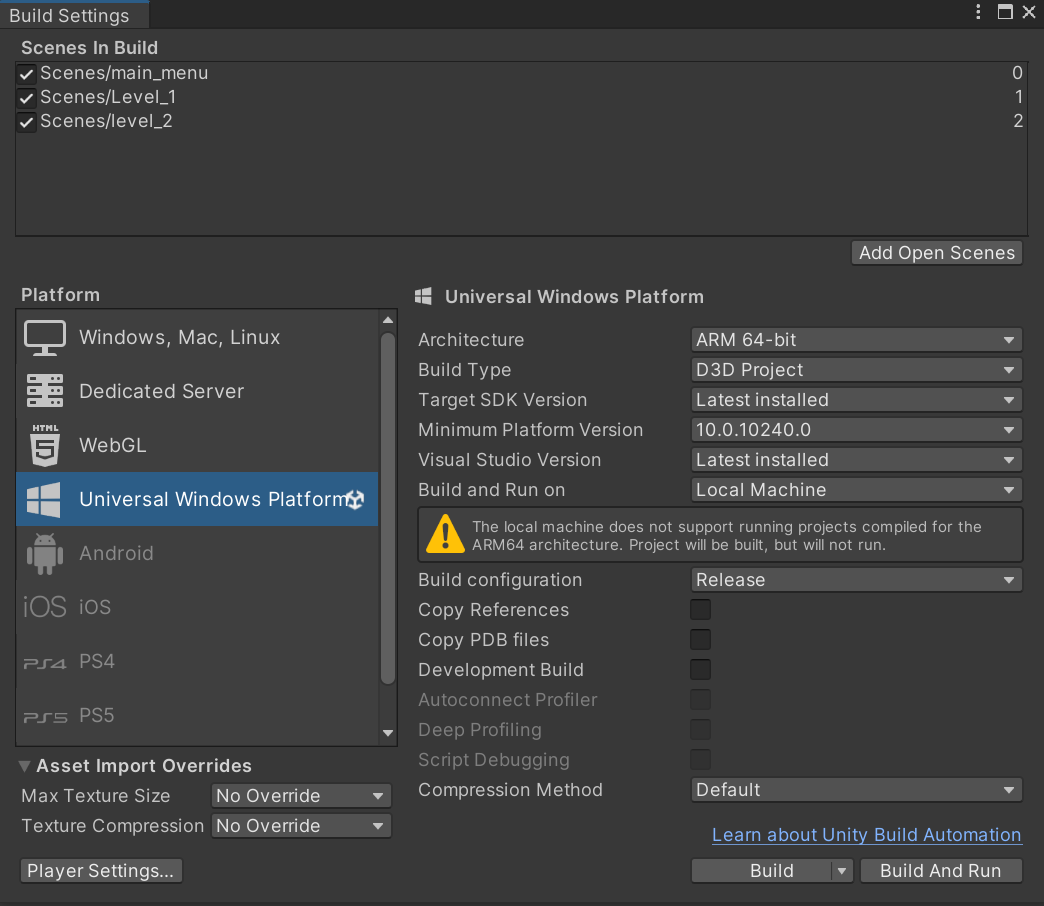
\includegraphics[scale=0.6]{images/build}
    \caption{Build-Einstellungen in Unity}
    \label{fig:build-settings}
\end{figure}

Nach einem erfolgreichen Build erhalten Sie einen Ordner mit den benötigten Dateien für das Deployment. Der nächste
Schritt erfolgt in der Visual Studio Solution, in unserem Fall \textit{AARIE.sln}. Nach dem Öffnen der Datei müssen die
Konfiguration auf \textit{Release} und die Plattform auf \textit{ARM64} eingestellt werden. Nachdem die Konfigurationen
vorgenommen wurden, muss die \textit{Machine Name} auf die lokale IPv4-Adresse der HoloLens gesetzt werden. Dies erfolgt in
den \textit{Projekteigenschaften} unter Debugging. Die IP-Adresse der HoloLens kann auf der Brille in den \textit{Einstellungen}
unter \textit{Netzwerk} gefunden werden.

Außerdem muss der \textit{Authentication Mode} auf \textit{Universal (Unencrypted Protocol)} gesetzt werden, um
sicherzustellen, dass die Kommunikation zwischen dem Computer und der HoloLens reibungslos erfolgt.

Nachdem alle Einstellungen vorgenommen wurden, kann die Anwendung auf die HoloLens deployt werden. Dazu muss die
Solution mit \textit{Start without Debugging} gestartet werden. Nach einem längeren Ladevorgang wird die Anwendung auf der
HoloLens geladen und gestartet.

Falls die Anwendung beendet wird, kann sie auf der HoloLens unter
\textit{Start} $\rightarrow$ \textit{Alle Apps} $\rightarrow$ \textit{AARIE} erneut gestartet werden.
Falls Änderungen an der Anwendung auf den Computern vorgenommen wurden, muss der gesamte Prozess erneut durchgeführt werden.
Die Anwendung wird nicht automatisch aktualisiert!

\subsubsection{Erstmaliges Deployment}
Beim erstmaligen Deployment auf die HoloLens kann es zu Problemen kommen, die durch die Authentifizierung der HoloLens
verursacht werden. In diesem Fall muss der neue Computer sich auf der HoloLens erneut authentifizieren. Dazu werden Sie nach
dem Starten des Deployments aufgefordert. Auf dem Computer wird ein Authentifizierungscode angezeigt, der auf der HoloLens unter
\textit{Einstellungen} $\rightarrow$ \textit{Update & Sicherheit} $\rightarrow$ \textit{Für Entwickler} $\rightarrow$ \textit{Koppeln}
eingegeben wird. Nachdem die Authentifizierung erfolgreich abgeschlossen wurde, kann das Deployment erneut gestartet werden.


\section{Objektdesign mit Blender} \marginpar{\small\(\rightarrow\) LAMPEL}
Das Entwerfen von 3D-Objekten mit Blender erfordert ein Verständnis der Struktur und Funktionalität dieser leistungsstarken
Software. Im Folgenden wird erläutert, wie Blender aufgebaut ist, auf welche Aspekte bei der Gestaltung der Objekte geachtet
wurde und welche Add-ons und Plug-ins verwendet wurden, um den Designprozess zu optimieren.

\subsection{Optimierung für Augmented Reality}
Der Entwurf von 3D-Objekten mit Blender erfordert ein systematisches Vorgehen, insbesondere im Zusammenhang mit der
Optimierung für Augmented Reality (AR). Im Folgenden werden spezifische Aspekte dieses Prozesses beleuchtet, darunter
die Polygonreduktion und die Texturoptimierung.

\subsubsection{Polygonreduktion}
Die Polygonreduktion ist eine Technik, die darauf abzielt, die Anzahl der Polygone in einem 3D-Modell zu reduzieren, um
die Belastung der Hardware zu verringern, insbesondere bei Echtzeitanwendungen wie Computerspielen oder Simulationen.
Eine effiziente Polygonreduktion ermöglicht eine bessere Leistung und eine schnellere Darstellung der Modelle auf
verschiedenen Plattformen.

In der Computergrafik steht die Anzahl der Polygone eines Modells in direktem Zusammenhang mit dem benötigten Speicherplatz
und der Rechenleistung. Je mehr Polygone ein Modell hat, desto mehr Daten müssen verarbeitet und gerendert werden, was
zu höheren Anforderungen an die Hardware führt. Durch eine Reduzierung der Polygone können diese Ressourcen effizienter
genutzt werden, ohne dass die visuelle Qualität des Modells wesentlich beeinträchtigt wird.

Werkzeuge wie der Decimate Modifier in Blender bieten Möglichkeiten, die Anzahl der Polygone automatisch zu reduzieren
und gleichzeitig visuelle Artefakte zu minimieren. Dennoch ist es ratsam, bereits während des Modellierungsprozesses
darauf zu achten, keine unnötigen zusätzlichen Unterteilungen zu erzeugen, um eine optimale Ausgangsbasis für die
Polygonreduktion zu schaffen.

Die Polygonreduktion ist ein wichtiger Bestandteil der 3D-Modellierung und -Optimierung, da sie dazu beiträgt, die Leistung
von Anwendungen zu verbessern und die Benutzererfahrung zu optimieren. Durch eine sorgfältige Anwendung dieser Technik
können qualitativ hochwertige 3D-Modelle erstellt werden, die sowohl ästhetisch ansprechend als auch effizient zu verarbeiten
sind.

\subsubsection{Texturenoptimierung}
Die Optimierung von Texturen ist ein wesentlicher Bestandteil der Gestaltung von 3D-Modellen für Augmented Reality
(AR)-Anwendungen, da sie einen direkten Einfluss auf die Benutzererfahrung haben. Bei der Auswahl geeigneter Texturen
muss der Auflösung besondere Aufmerksamkeit geschenkt werden, insbesondere im Hinblick auf die begrenzte Leistungsfähigkeit
von AR-Geräten wie der Hololens 2.

Während des Texturierungsprozesses wurde die Hololens 2 mehrfach in die Texturen integriert, um mögliche Leistungseinbußen
zu identifizieren. Wurden Beeinträchtigungen festgestellt, wurden entsprechende Anpassungen an den Texturen vorgenommen.
Dies beinhaltete entweder die Suche nach alternativen Texturen oder die Komprimierung der vorhandenen Texturen, um eine
geringere Auflösung zu erreichen. In einigen Fällen wurde auch der Reflexionsgrad angepasst, insbesondere wenn das Modell
poliertes Metall oder ähnliches enthielt, um die Leistung der AR-Anwendung zu optimieren.

Die Texturoptimierung ist ein iterativer Prozess, der eine ausgewogene Berücksichtigung der visuellen Qualität und der
Leistungsfähigkeit der AR-Plattform erfordert. Durch die gezielte Optimierung von Texturen können AR-Anwendungen erstellt
werden, die eine ansprechende visuelle Darstellung bieten und gleichzeitig ein flüssiges und immersives Benutzererlebnis
gewährleisten.

\subsection{Export- und Integrationsprozess}
In diesem Abschnitt wird der Export- und Integrationsprozess für 3D-Modelle beschrieben, beginnend mit der Auswahl des
geeigneten Dateiformats und der Berücksichtigung verschiedener Koordinatensysteme.

Der Export- und Integrationsprozess ist ein entscheidender Schritt bei der Übertragung von 3D-Modellen aus der Konstruktions-
oder Modellierungssoftware in eine Zielumgebung, sei es eine Spiele-Engine, eine Virtual-Reality-Plattform oder eine AR-Anwendung.
Dieser Prozess umfasst mehrere Schritte, um sicherzustellen, dass das Modell korrekt dargestellt und funktional in die
Zielumgebung integriert wird.

\subsubsection{Dateiformat}
Als Dateiformat für den Export von 3D-Modellen in diesem Projekt wurde das von Autodesk entwickelte Filmbox-Format (FBX)
gewählt. FBX wurde aufgrund seiner weit verbreiteten Unterstützung und seiner Fähigkeit, umfassende Informationen über
geometrische Formen, Materialien, Animationen und andere Szenendaten zu speichern, ausgewählt.

FBX ist ein proprietäres Format, das speziell für den Austausch von 3D-Inhalten zwischen verschiedenen Anwendungen
entwickelt wurde. Es bietet eine hierarchische Struktur, die es ermöglicht, komplexe Szenen zu organisieren und zu
übertragen. Diese Struktur umfasst Knoten, die verschiedene Elemente der 3D-Szene repräsentieren, wie Geometrie,
Materialien, Animationen, Kameras und Lichtquellen. \footnote{Autodesk \cite{FBX. Getting started}}

Durch die Verwendung von FBX können 3D-Modelle nahtlos zwischen verschiedenen Softwareanwendungen und Plattformen
ausgetauscht werden, was die Zusammenarbeit und Integration in Projekten wie diesem, das Unity als Engine verwendet,
erleichtert. Die Wahl des FBX-Formats bietet somit eine solide Grundlage für einen effizienten Workflow und eine
erfolgreiche Umsetzung des Projekts.

\subsubsection{Koordinatensysteme}
Die Berücksichtigung und korrekte Handhabung von Koordinatensystemen während des Modellierungsprozesses ist ein
entscheidender Aspekt für die nahtlose Integration von 3D-Modellen in verschiedene Anwendungen. In diesem Projekt
wurden spezifische Maßnahmen ergriffen, um potenzielle Probleme im Zusammenhang mit Koordinatensystemen zu minimieren.

Während der Modellierung wurden alle Objekte im Koordinatenursprung platziert, um sicherzustellen, dass beim Export
der Modelle nach Unity keine Komplikationen hinsichtlich Platzierung und Ausrichtung auftreten. Diese Vorgehensweise
trägt dazu bei, mögliche Diskrepanzen zwischen den Koordinatensystemen der Modellierungssoftware und der Zielplattform
zu vermeiden, was den Integrationsprozess vereinfacht und beschleunigt.

Darüber hinaus wurden alle Modelle in der gleichen Ausrichtung modelliert, um zusätzliche Anpassungen in Unity zu
vermeiden. Diese konsistente Orientierung stellt sicher, dass alle Modelle bereits in einer standardisierten
Orientierung vorliegen, was die Notwendigkeit weiterer manueller Eingriffe minimiert und einen reibungsloseren
Arbeitsablauf gewährleistet.

Für den Fall, dass Modelle dennoch mit einer falschen Rotation exportiert wurden, wurden entsprechende Korrekturen
direkt im Unity Inspector vorgenommen. Diese Nachjustierung ermöglicht es, eventuelle Fehler in der Ausrichtung der
Modelle schnell und effizient zu beheben, ohne den Modellierungsprozess zu unterbrechen oder zusätzlichen Aufwand zu
verursachen.

Insgesamt zeigt die Berücksichtigung von Koordinatensystemen während des gesamten Workflows einen proaktiven Ansatz
bei der Modellierung und Integration von 3D-Objekten. Die Umsetzung dieser Maßnahmen wird die Konsistenz und Effizienz
des Projekts verbessern und gleichzeitig mögliche Komplikationen im Zusammenhang mit Koordinatensystemen effektiv
vermeiden.

\subsection{Add-Ons und Plugins}
Während der Modellierungsphase wurden einige Add-ons und Plug-ins verwendet, um die Erfahrung zu verbessern und die
Modellierung effizienter zu gestalten. Im folgenden Abschnitt werden die wichtigsten Add-ons und Plug-ins erläutert.

\subsubsection{Looptools: Optimierung von Topologie und Oberflächen}
Das Add-on Looptools für Blender stellt eine wichtige Ergänzung für die Flächenmodellierung und Topologieoptimierung dar.
Insbesondere bei der Umwandlung von rechteckigen oder quadratischen Flächen in kreisförmige Flächen erweist sich dieses
Werkzeug als äußerst nützlich.

Als Hauptwerkzeug wurde das so genannte \textit{Circle}-Werkzeug verwendet, das speziell zur Lösung des oben genannten Problems
entwickelt wurde. Mit dem Circle-Werkzeug können rechteckige Flächen unter Berücksichtigung der Topologie und der
Anzahl der Polygone nahtlos in kreisförmige Flächen umgewandelt werden.

Das Circle-Werkzeug bietet verschiedene Einstellungsmöglichkeiten, um die extrahierte Figur optimal für den jeweiligen
Zweck zu konfigurieren. Die wichtigsten Konfigurationspunkte sind

\begin{itemize}
    \item \textbf{Best Fit:} Dieses Werkzeug berechnet einen Kreis mit Hilfe einer nichtlinearen Methode der kleinsten
    Quadrate. Dadurch wird sichergestellt, dass der berechnete Kreis optimal zu den ausgewählten Eckpunkten passt. \footnote{Blender \cite{LoopTools}}
    \item \textbf{Fit Inside:} Mit dieser Option wird der Kreis so berechnet, dass kein Eckpunkt vom Kreismittelpunkt
    entfernt wird. Dies ist besonders nützlich, wenn die Topologie des umgebenden Mesh erhalten bleiben soll.
\end{itemize}

Zusätzlich ermöglicht das Circle-Werkzeug die Anpassung weiterer Konfigurationsparameter wie Radius und Regularität, um
die extrahierte Figur feiner abzustimmen und besser an individuelle Anforderungen anzupassen.

Insgesamt trägt das Looptools Add-On dazu bei, den Modellierungsprozess effizienter zu gestalten und die Qualität der
resultierenden Modelle zu verbessern, indem es eine Reihe präziser und flexibler Werkzeuge für die Topologie- und
Flächenoptimierung bereitstellt.

\subsubsection{Images as Planes: Effiziente Integration von Texturen}
Das Addon Images as Planes spielt eine entscheidende Rolle in der Modellierungspraxis, insbesondere im Bereich der
realistischen Modellierung.

Das Hauptanwendungsgebiet dieses Add-ons liegt in der Möglichkeit, Vorschaubilder für die Modellierung hinter Objekten
zu platzieren, um eine realistischere und präzisere Modellierung zu ermöglichen. Diese Funktion bietet die Möglichkeit,
reale Bilder als Referenz in Blender-Szenen zu integrieren und als Hintergrund für die Modellierung zu verwenden. Durch
die direkte Integration von Bildern in die Arbeitsumgebung können feine Details und Proportionen besser beurteilt und
reproduziert werden, was zu einer verbesserten Qualität der Modelle führt.

Die Verwendung von \textit{Images as Planes} trägt somit wesentlich zur Erhöhung der Genauigkeit und Realitätsnähe der
Modellierung bei, indem sie eine effiziente Möglichkeit bietet, reale Referenzen in den Modellierungsprozess zu integrieren.
Diese Funktion ist besonders nützlich bei der Modellierung von Objekten, die auf realen Vorbildern basieren, da sie es
dem Modellierer ermöglicht, direkt aus Bildern heraus zu arbeiten und so einen höheren Detaillierungsgrad zu erreichen.

Insgesamt ist das Addon Images as Planes ein unverzichtbares Werkzeug für die realistische Modellierung in Blender,
das die Effizienz und Qualität des Modellierungsprozesses erheblich verbessert. Durch die nahtlose Integration von Bildern
als Hintergrundreferenzen können Designer ihrer Kreativität freien Lauf lassen und präzise Modelle mit realistischen
Details erstellen.

\subsection{Modi}
In Blender stehen verschiedene Modi zur Verfügung, mit denen unterschiedliche Aspekte eines Objekts bearbeitet und
manipuliert werden können. Diese verschiedenen Modi in Blender bieten eine umfassende Palette an Werkzeugen und Funktionen,
mit denen die Benutzer ihre 3D-Modelle auf vielfältige Weise bearbeiten und verfeinern können. \footnote{Blender \cite{Modi}}

\subsubsection{Object-Modus}
Der Object-Modus ist der Standardmodus in Blender und steht für alle Arten von Objekten zur Verfügung. In diesem Modus
können grundlegende Transformationen wie Positionierung, Rotation und Skalierung sowie Duplizierung und andere
Objekteigenschaften bearbeitet werden.

\subsubsection{Edit-Modus}
Der Edit-Modus ist ein spezialisierter Modus zum Bearbeiten der Form eines Objekts. Hier können mithilfe verschiedener
Werkzeuge und Kontrollpunkte einzelne Vertices, Kanten und Flächen des Objekts bearbeitet werden. Dies ermöglicht
detaillierte Manipulationen und Anpassungen an der Geometrie des Objekts, was insbesondere für die Modellierung von
entscheidender Bedeutung ist. \footnote{Blender \cite{Vertices}}

\subsubsection{Texture-Paint-Modus}
Der Texture-Paint-Modus ist ein spezieller Modus, der es ermöglicht, Texturen direkt auf das Mesh
eines Objekts zu malen. Dieser Modus ist ausschließlich auf das Bearbeiten von Meshes beschränkt und bietet eine intuitive
Möglichkeit, Texturen im 3D-Viewport zu zeichnen und zu bearbeiten. Durch die direkte Malerei auf dem Objekt können
komplexe Texturen und Oberflächeneffekte einfach erstellt und angepasst werden. \footnote{Blender \cite{Mesh}}

\subsection{Hierarchie}
In der 3D-Modellierung bezieht sich Hierarchie auf die strukturierte Organisation von Objekten innerhalb einer Szene
oder eines Modells. Diese Hierarchie wird oft durch eine Baumstruktur dargestellt, in der übergeordnete Objekte
untergeordnete Objekte enthalten können. Die Hierarchie spielt eine entscheidende Rolle bei der Verwaltung und
Manipulation von Objekten sowie bei der Definition von Beziehungen zwischen ihnen.

\begin{itemize}
    \item \textbf{Eltern-Kind-Beziehungen:} Übergeordnete Objekte werden oft als Eltern bezeichnet und enthalten
    untergeordnete Objekte, die als Kinder bezeichnet werden. Diese Beziehung ermöglicht es, Transformationen wie
    Verschieben, Drehen und Skalieren auf das übergeordnete Objekt anzuwenden, welche dann auf seine untergeordneten
    Objekte übertragen werden. Diese Technik ist besonders nützlich für komplexe Strukturen wie Roboterglieder oder
    hierarchische Modelle.
    \item \textbf{Gruppierung:} Objekte können hierarchisch gruppiert werden, um sie logisch zu organisieren und ihre
    Handhabung zu erleichtern. Durch die Gruppierung ist es möglich, mehrere Objekte gleichzeitig auszuwählen, zu
    verschieben oder zu bearbeiten, ohne jedes einzelne Objekt separat manipulieren zu müssen.
\end{itemize}
Die Hierarchie ist ein grundlegendes Konzept in der 3D-Modellierung. Sie ermöglicht eine effiziente Organisation und
Manipulation von Objekten. Durch die kluge Nutzung von Hierarchien können komplexe Modelle erstellt und verwaltet werden.
Dies führt zu einer effizienteren Arbeitsweise und einer verbesserten Qualität der Ergebnisse.

\subsection{Modifier}
Modifier sind Werkzeuge oder Operationen, die auf Objekte in der 3D-Modellierung angewendet werden, um ihr Aussehen oder
Verhalten zu verändern, ohne die zugrunde liegende Geometrie dauerhaft zu ändern. Sie ermöglichen es den Modellierenden,
komplexe Effekte zu erzielen, ohne manuell jeden einzelnen Aspekt des Modells zu bearbeiten. Modifier sind ein wichtiger
Bestandteil vieler 3D-Modellierungssoftware und bieten eine Vielzahl von Funktionen zur Verbesserung des Modellierungsprozesses.
Die Verwendung von Modifiern bringt mehrere Vorteile mit sich:

\begin{itemize}
    \item \textbf{Non-destructive Bearbeitung:} Modifier werden auf das Modell angewendet, ohne die ursprüngliche
    Geometrie zu verändern. Dies ermöglicht es, Änderungen vorzunehmen und bei Bedarf zum ursprünglichen Zustand
    zurückzukehren.

    \item \textbf{Effizienzsteigerung:} Durch die Verwendung von Modifiern können komplexe Effekte und Veränderungen mit
    weniger manuellem Aufwand erreicht werden. Dies führt zu einem effizienteren Modellierungsprozess und spart
    Zeit und Ressourcen.

    \item \textbf{Experimentierfreude:} Da Modifier nicht-destruktiv sind, können sie leicht hinzugefügt, angepasst oder
    entfernt werden. Dies ermutigt dazu, verschiedene Optionen auszuprobieren und kreativ zu experimentieren, ohne
    Angst vor irreversiblen Änderungen haben zu müssen.
\end{itemize}

Beispiele für Modifier sind Subdivision Surface, Mirror, Bevel, Array und Boolean. Jeder Modifier hat spezifische
Anwendungsfälle und ermöglicht es den Modellierenden, eine Vielzahl von Effekten zu erzielen, von der Glättung von
Kanten bis zur Erstellung von komplexen Wiederholungsmustern.

Modifier sind ein wichtiger Bestandteil der 3D-Modellierung. Sie bieten eine flexible und leistungsstarke Möglichkeit,
Objekte zu bearbeiten und zu verbessern, ohne die Integrität des Modells zu beeinträchtigen. Die Verwendung von Modifiern
kann den Modellierungsprozess rationalisieren und die Kreativität der Modellierenden fördern.

% vielleicht sachen dazu wie polygonanzahl oder arbeitsstunden oder sowas idk
\subsection{Modellierung von Gegenständen für das Projekt}
Dieser Abschnitt beschreibt die für das Projekt in Blender modellierten Gegenstände sowie die dabei aufgetretenen Herausforderungen.

Zu Beginn des Projekts musste eine wichtige Entscheidung getroffen werden, nämlich wie viele Objekte modelliert werden
sollten. Es war wichtig, eine ausgewogene Anzahl zu wählen, die das Spiel nicht überladen, aber dennoch eine
Herausforderung für die Spieler darstellt. Nach eingehenden Recherchen und internen Abstimmungen wurde sich auf 11
Gegenstände geeinigt. Diese sollten alltägliche Gegenstände eines Schülers der HTBLuVA darstellen und den Spielern
einen Einblick in den Schulalltag bieten.

\subsubsection{Taschenrechner}
Um den Modellierungsprozess am Beispiel des Taschenrechners zu veranschaulichen, werden spezifische Schritte und
Überlegungen während des Prozesses erläutert. Der Prozess begann mit der Idee, den Taschenrechner als Teil des Projekts
zu integrieren. Anschließend wurde der Modellierungsumfang und die Art des Taschenrechners festgelegt. Dabei diente das
Casio FX-991 ESPLUS Modell als Referenz für das zu erstellende Modell.

\subsubsection*{Ausgangslage}
Im Modellierungsprogramm Blender war das Standardprojekt als Ausgangslage zu sehen. Es wurde bereits geringfügig
angepasst. Die Standardkamera und Lichtquelle, die für das Rendering innerhalb von Blender verwendet werden, wurden
entfernt, da sie für das finale Projekt in Unity nicht benötigt werden und unnötige Komplikationen verursachen könnten.
Je nach Anforderung des Modells wird eine geeignete Grundform wie beispielsweise ein Würfel, eine Fläche oder ein Zylinder
erstellt, um darauf aufbauend mit der eigentlichen Modellierung zu beginnen.

\begin{figure}[H]
    \centering
    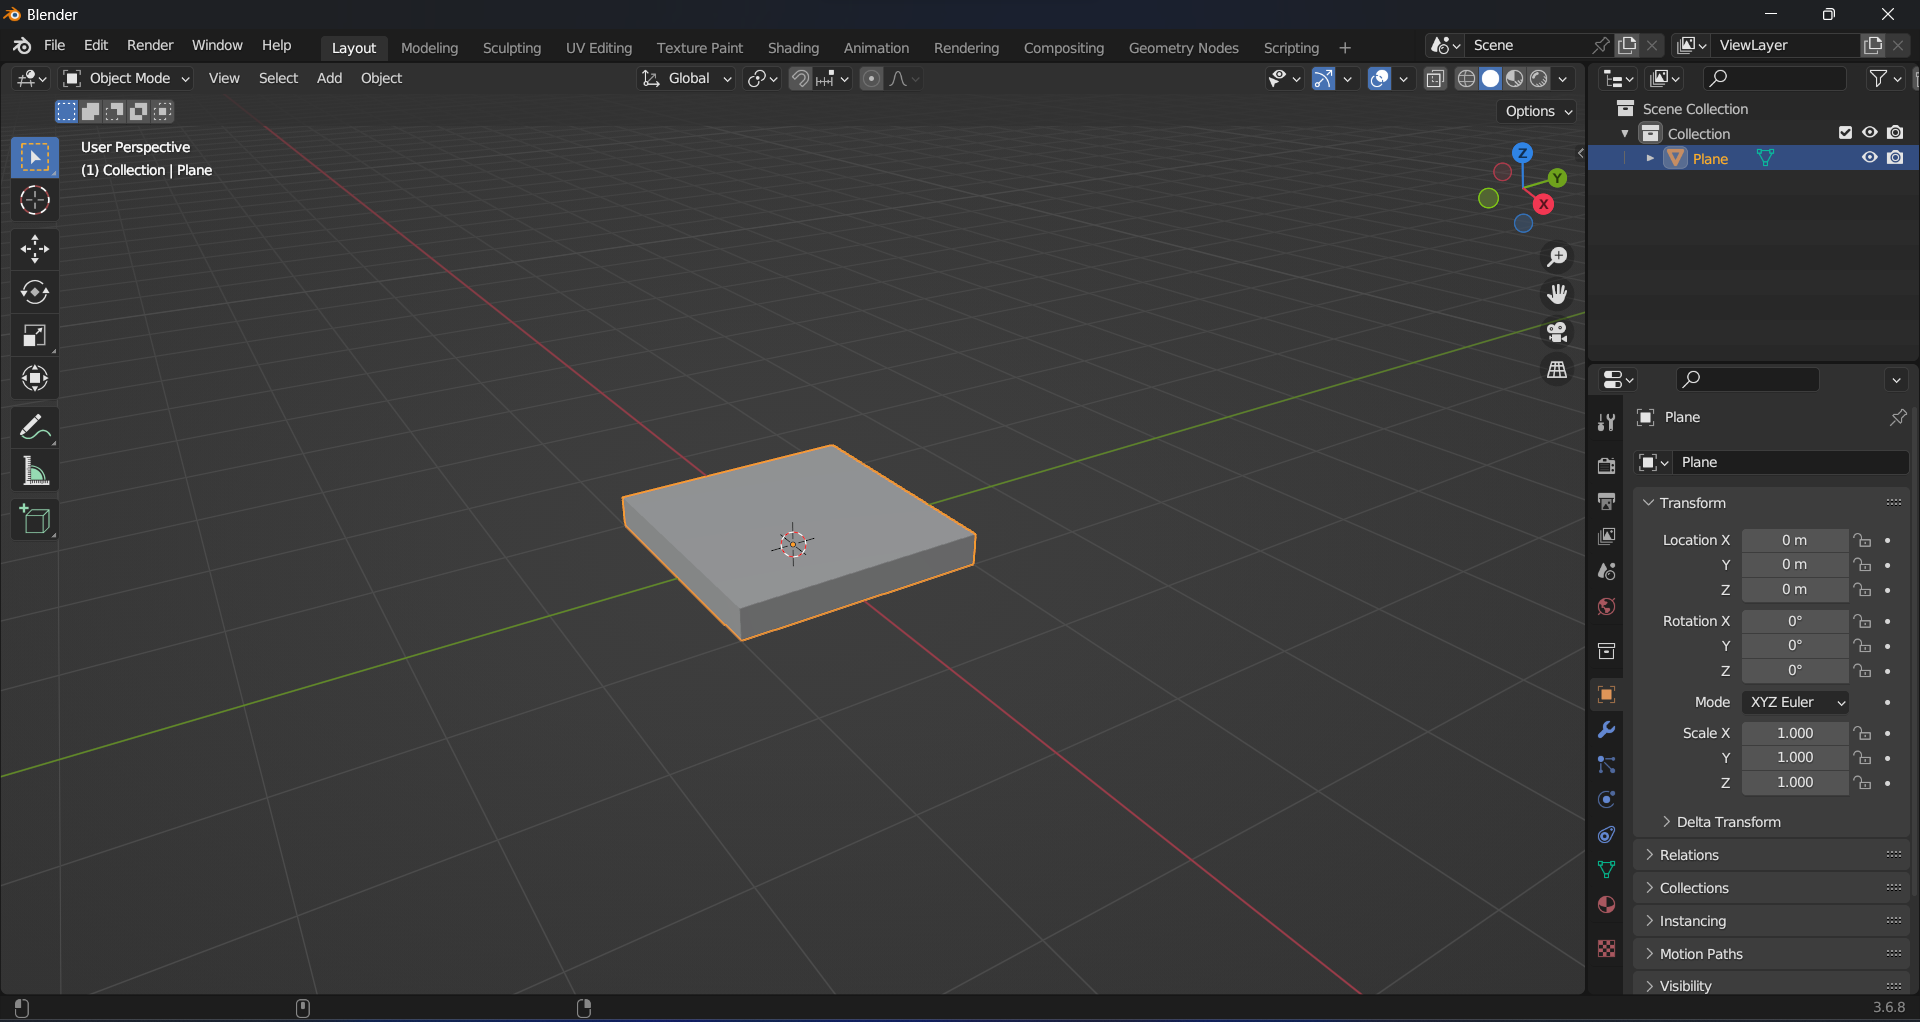
\includegraphics[width=1\textwidth]{images/AusgangslageTaschenrechner.png}
    \caption{Ausgangslage innerhalb von Blender}
    \label{fig:Ausgangslage}
\end{figure}

Durch diesen Prozess der Initiierung wurde die Grundlage für die folgenden Schritte der Modellierung gelegt, die in
weiteren Abschnitten detaillierter beschrieben werden.

\subsubsection*{Erste Schritte nach der Erstellung}
Nach Auswahl eines geeigneten Referenzbildes für das Taschenrechnermodell wurde dieses mithilfe des
Add-Ons \textit{Images as Planes} in Blender eingefügt. Das Bild dient als Leitfaden für die Modellierung und wurde
unterhalb des bereits vorhandenen Objekts platziert. Um eventuelle Unregelmäßigkeiten im Design zu vermeiden, wurde der
Mirror Modifier aufgrund der symmetrischen Form des Taschenrechners angewendet. Durch diese Maßnahme werden alle
Modellierungsaktionen, die auf einer Seite durchgeführt werden, automatisch auf die andere Seite gespiegelt. Dadurch
wird die Effizienz des Modellierungsprozesses erhöht.

Im Anschluss begann die Modellierung durch Extrudieren eines Eckpunkts der Fläche, um grob der Form des Referenzbildes zu folgen.

\begin{figure}[H]
    \centering
    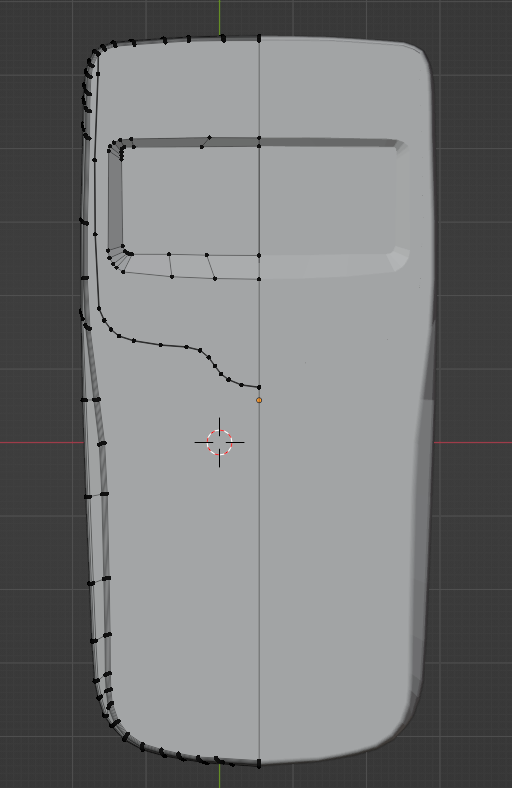
\includegraphics[width=0.4\textwidth]{images/basis.png}
    \caption{Taschenrechner mit Buttons in Blender}
    \label{fig:Basis}
\end{figure}


Nach Abschluss dieser groben Modellierungsschritte entstand das Grundgerüst des Taschenrechnermodells, wie in
Abbildung \ref{fig:Basis} dargestellt. Die verschiedenen Eckpunkte (Vertices) werden im Edit-Modus von Blender als
schwarze Punkte dargestellt. Durch den Mirror Modifier wird die Bearbeitung auf der linken Seite des Modells
automatisch auf die rechte Seite gespiegelt, was eine symmetrische Form gewährleistet. Um dem Modell mehr Tiefe zu
verleihen, wurde Extrudieren verwendet, um aus der ebenen Fläche eine dreidimensionale Struktur zu formen.

\subsubsection*{Extrahieren als Modellierungswerkzeug}
Extrahieren ist ein Werkzeug im Edit-Modus von Blender. Es dient dazu, ausgewählte Punkte zu duplizieren und zu verschieben,
während die ursprünglichen Punkte der Bearbeitungslinie erhalten bleiben.
Für die Verwendung des Extrahieren-Werkzeugs ist ein Verständnis der grundlegenden Konzepte des Edit-Modus in Blender
sowie eine präzise Auswahl der zu extrahierenden Punkte erforderlich, um die gewünschten Modifikationen am Modell
vorzunehmen. Während des Modellierungsprozesses ist es von entscheidender Bedeutung, unbeabsichtigte Extraktionen zu
vermeiden, da diese dazu führen können, dass duplizierte Vertices über bereits vorhandenen liegen. Dies kann nicht
nur die weitere Bearbeitung des Modells beeinträchtigen, sondern auch zu einer unnötigen Zunahme der Anzahl der
Vertices führen. \footnote{Blender \cite{Extrahieren}}

\subsubsection*{Weiterführung beim Taschenrechnermodell}
Als nächster Schritt steht die Modellierung der Knöpfe und anderer Funktionen des Taschenrechners an, um das Modell
weiter zu verfeinern und seinem realen Gegenstück näherzukommen. Dazu wird der \textit{Array}-Modifier verwendet, da
dieser es ermöglicht, ein Button-Modell zu entwerfen und dieses dann zu vervielfältigen. Dadurch wird die
Modellierungszeit enorm reduziert und die gleichmäßige Platzierung der Buttons verbessert.

\subsubsection*{Einschub Array-Modifier}
Der Array-Modifier in Blender ermöglicht die Erstellung einer Reihe von Kopien eines Basisobjekts. Jede Kopie wird dabei
auf eine vordefinierte Weise von der vorherigen Kopie versetzt. Der Modifier bietet eine Vielzahl von Optionen zur
Anpassung der Positionierung und Ausrichtung der Kopien.
Die grundlegenden Funktionen des Array-Modifiers umfassen die Möglichkeit, Vertices in benachbarten Kopien zusammenzuführen,
insbesondere wenn sie nahe beieinander liegen. Dadurch können nahtlose und konsistente Verbindungen zwischen den
einzelnen Kopien hergestellt werden.
Eine wichtige Option des Array-Modifiers ist der sogenannte \textit{Fit Type}, der angibt, wie das Objekt dupliziert
werden soll. Dies kann entlang einer Kurve, mit einer passenden Länge oder einer festgelegten Anzahl von Kopien erfolgen.
Darüber hinaus kann eine relative oder feste Verschiebung entlang der x-, y- oder z-Achse definiert werden, um die
Positionierung der Kopien weiter anzupassen.

\subsubsection*{Weiterführung beim Taschenrechnermodell}
\begin{figure}[H]
    \centering
    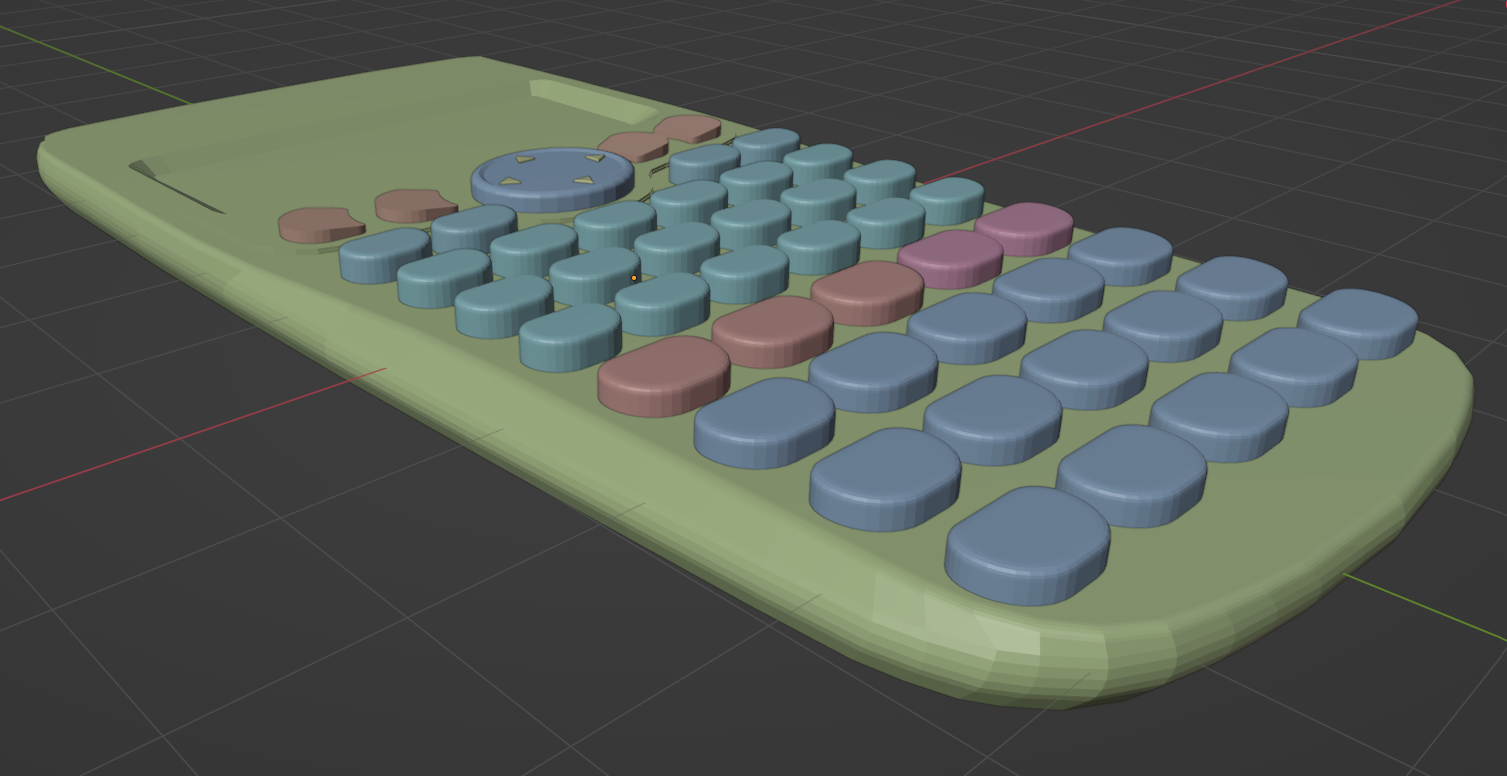
\includegraphics[width=0.8\textwidth]{images/taschenrechnermitbuttons.png}
    \caption{Taschenrechner mit Buttons in Blender}
    \label{fig:tcbuttons}
\end{figure}

Abbildung \ref{fig:tcbuttons} zeigt das Taschenrechnermodell in Blender mit den neu modellierten Buttons. Die
dargestellten Farben dienen lediglich als visuelle Hilfestellung im Blender-Editor und stellen keine inhärenten
Eigenschaften des Modells dar. Jedes neu erstellte Objekt wird automatisch mit einer zufälligen Farbe versehen, um eine
einfachere Unterscheidung innerhalb der Szene zu ermöglichen.

Einige der Buttons im Modell wurden mithilfe des Array-Modifiers vervielfältigt. Dies gilt insbesondere für Buttons, die
im Referenzbild die gleiche Größe, Funktion und Farbe aufweisen. Durch diese Technik ist es möglich, wiederkehrende
Elemente effizient zu modellieren, indem eine einzelne Vorlage kopiert und entsprechend der gewünschten Anordnung angepasst wird.

Der aktuelle Stand des Modells lässt darauf schließen, dass die Modellierung größtenteils abgeschlossen ist. Der nächste
Schritt besteht darin, dem Modell Farben oder Texturen hinzuzufügen, um ein realistischeres Aussehen zu erzielen. Dies
kann durch Anwendung von Materialien und Texturen im Renderprozess erreicht werden, um dem Modell visuelle Tiefe und
Detailtreue zu verleihen.

Die Fortführung des Modellierungsprozesses umfasst somit die Umsetzung der texturierten Oberfläche sowie mögliche
Feinanpassungen, um das Modell weiter zu verbessern und an die Referenzvorlage anzupassen.

\subsubsection*{Hierarchie des fertiggestellten Modells}
In Blender wird die Hierarchie eines Modells als Baumstruktur dargestellt. Dabei ermöglichen verschiedene Unterteilungen
und Kategorien eine übersichtliche Organisation. Die Struktur wird in Abbildung
\ref{fig:hierarchie} veranschaulicht. Das weiße Box-Symbol steht für eine Collection (Ordner).

\begin{figure}[H]
    \centering
    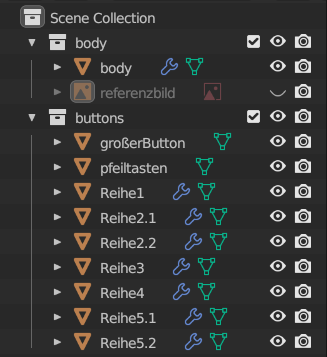
\includegraphics[width=0.5\textwidth]{images/hierarchietaschenrechner.png}
    \caption{Hierarchie des fertigen Taschenrechnermodells}
    \label{fig:hierarchie}
\end{figure}

\begin{itemize}
    \item Die \textbf{Scene Collection} ist die oberste Ebene, die das gesamte Modell enthält.
    \item Die \textbf{Body Collection} enthält das Hauptmodell des Taschenrechners, also die grundlegende Form.
    \item Die \textbf{Buttons Collection} umfasst alle Buttons, die auf dem Taschenrechner abgebildet sind.
    \item Die untergeordnete Struktur mit den orangefarbenen Dreiecken repräsentiert die eigentlichen Objekte innerhalb der jeweiligen Collections.
    \item Das \textbf{Referenzbild} ist ein importiertes Bild, an dem sich während des Modellierens orientiert wurde.
\end{itemize}

In Abbildung \ref{fig:hierarchie} ist zu erkennen, dass ein Objekt ausgegraut ist. Dies bedeutet in dem Fall, dass das
Objekt ausgeblendet wurde, da das Hauptmodell bereits fertiggestellt wurde und das Referenzbild nicht mehr benötigt wird.
Das Referenzbild kann jedoch bei Bedarf aktiviert werden, beispielsweise zu Hilfe- oder Veranschaulichungszwecken.

Die hierarchische Darstellung der Elemente erleichtert die Organisation und Bearbeitung des Modells. Eine klare
Strukturierung der verschiedenen Komponenten ermöglicht eine effiziente Arbeitsweise und hilft, den Überblick über die
einzelnen Teile zu behalten.

\subsubsection*{Textur und Farbe des Taschenrechnermodells}
Für die Texturierung und Farbgebung des Modells wurde sich eng an dem Referenzbild orientiert.
Das \textit{Eye-Dropper}-Werkzeug in Blender ermöglichte es, Farben gezielt aus dem Referenzbild auszuwählen und auf das
entsprechende Modell anzuwenden. Durch Klicken auf einen bestimmten Bereich des Referenzbildes wurde die Farbe erfasst
und dann auf den entsprechenden Bereich des Modells übertragen.

Dieser Prozess wurde für jedes Element des Modells durchgeführt, um eine genaue Anpassung an die Farben und Texturen des
Referenzbildes zu erreichen. Die Verwendung des Eye-Dropper-Werkzeugs ermöglichte eine präzise und konsistente Umsetzung
der Farbgebung und trug dazu bei, dass das Modell möglichst authentisch und realitätsnah aussieht. Um noch bessere und
realitätsnähere Textur zu gewährleisten, wurde ein Vorgang Namens \textit{UV-Mapping} durchgeführt.

%literatur https://docs.blender.org/manual/en/latest/modeling/meshes/editing/uv.html
%literatur https://all3dp.com/2/blender-uv-mapping-simply-explained/
%literatur https://de.wikibooks.org/wiki/Blender_Dokumentation:_UV-Mapping
\subsubsection*{UV-Mapping}
\textit{UV-Mapping} ist ein wichtiger Schritt im Texturierungsprozess von 3D-Modellen. Dabei werden Texturen auf
dreidimensionale Objekte projiziert. Die Bezeichnungen \textit{U} und \textit{V} stehen dabei für die beiden
Koordinatenachsen im zweidimensionalen Raum. In Blender gibt es dafür einen eigenen Editor mit einer spezifischen
Benutzeroberfläche.

Während der Modellierung des Taschenrechnermodells wurde \textit{UV-Mapping} genutzt, um Texturen detailgetreu von einem
Referenzbild auf die einzelnen Knöpfe und Tasten des Modells zu übertragen. Dieser Prozess ermöglicht es, die Beschriftungen
und andere Details automatisch von der Textur abzuleiten, anstatt sie manuell für jedes Element erstellen zu müssen.

\begin{figure}[H]
    \centering
    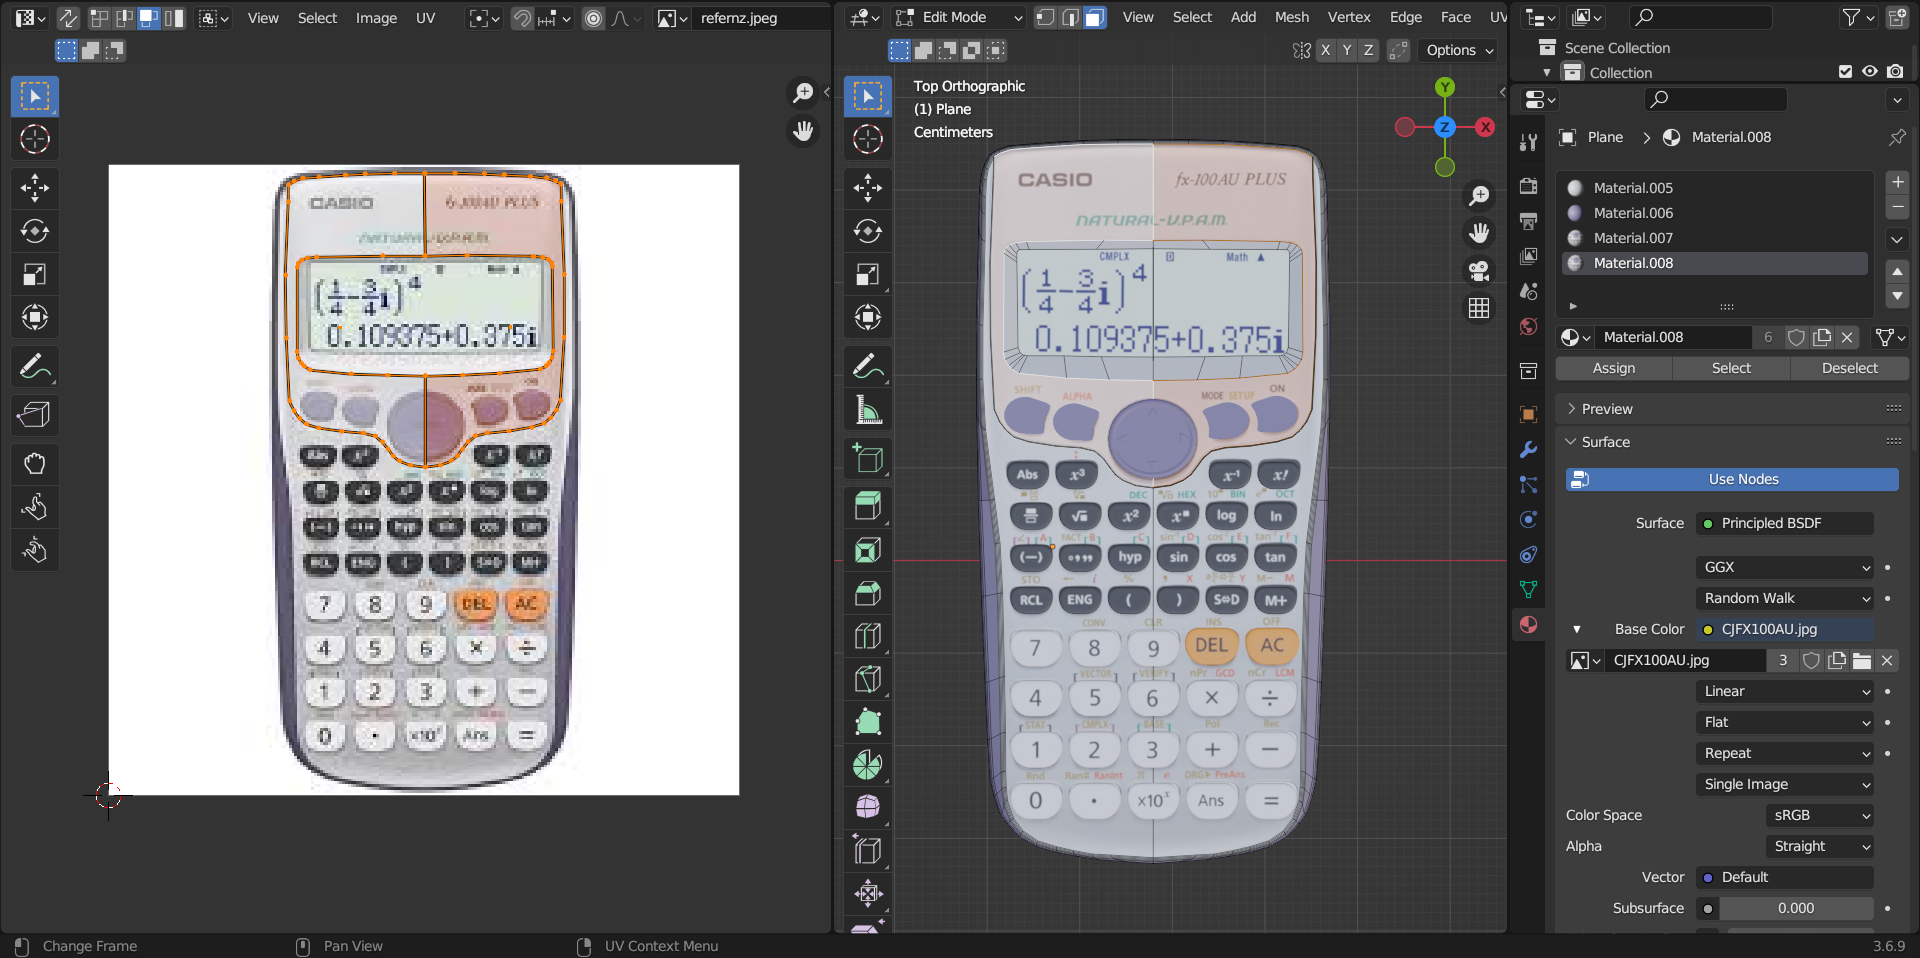
\includegraphics[width=1\textwidth]{images/uvmappingeditor.png}
    \caption{Ansicht des UV-Editing Editors in Blender}
    \label{fig:uvmappingeditor}
\end{figure}

Die Abbildung \ref{uvmappingeditor} zeigt den \textit{UV-Editing-Editor} in Blender. Mit diesem Editor können die UV-Maps der 3D-Modelle
bearbeitet werden, indem die 3D-Geometrie auf eine zweidimensionale Ebene projiziert wird, um die Positionierung der
Texturen zu steuern.

Als Beispiel wurde der obere Teil des Taschenrechners rund um den Bildschirm ausgewählt. Zunächst wird dem Bereich
ein neues Material zugewiesen, das die Basisfarbe des Referenzbildes enthält. Anschließend wird das Referenzbild als
Texturhintergrund im Editor ausgewählt, um es anzuzeigen.

Der nächste Schritt besteht darin, die ausgewählten Flächen des Modells aufzuteilen, denn die Erstauswahl in Blender
legt die einzelnen Flächen übereinander. Dies geschieht durch Auswahl der Flächen im Editor und Anwendung der
\textit{UV-Unwrap}-Funktion in Blender.

Nach dem \textit{UV-Unwrappen} werden die Flächen im Editor positioniert, um die Texturen und Beschriftungen korrekt auf
das Modell zu projizieren, ohne dass sie abgeschnitten oder verzerrt wirken. Dieser Prozess ist zeitaufwendig, da er für
jedes einzelne Element des Modells wiederholt werden muss. Dabei muss auch auf korrekte Skalierungen geachtet werden, um
eine einheitliche Darstellung zu gewährleisten.

\textit{UV-Mapping} ist somit ein entscheidender Schritt bei der Erstellung realistischer 3D-Modelle, da es eine präzise
Texturierung und Gestaltung ermöglicht.

\subsubsection{Restlichen Modelle}
\subsubsection*{Ping-Paket-Modell}
Das Ping-Paket-Modell wurde speziell für didaktische Zwecke auf Level 1 konzipiert, um Spielern das grundlegende Konzept
eines Daten-Pings zu veranschaulichen. Es dient dazu, die Übertragung von Daten zwischen zwei Endpunkten, beispielsweise
Laptops, zu visualisieren. Das Modell besteht im Wesentlichen aus einem simplen Quader, ergänzt durch Details wie
Paketklebeband, um eine realistische Darstellung zu erreichen. Bei der Texturierung wurde ein Amazon-Paket als Referenz verwendet.

\subsubsection*{Laptop-Modell}
Der Laptop stellt einen unverzichtbaren Gegenstand auf Level 2 dar und ist ein essenzielles Werkzeug für Schüler ab der
3. Klasse. Bei der Modellierung wurden zusätzliche Details wie USB-Ports und der Laptopständer berücksichtigt. Um den
Aufwand zu minimieren, wurde der Laptop im geschlossenen Zustand modelliert, wodurch die Komplexität von Tastatur und
Bildschirm vermieden wurde. Die Referenz für das Modell lieferte ein reales Laptop-Exemplar eines Projektmitglieds.

\subsubsection*{Router-Modell}
Die Modellierung des Routers war eine iterative Aufgabe, die mehrere Versionen erforderte, um ein realistisches und
ansprechendes Modell zu erzielen. Das finale Modell repräsentiert einen Gaming-Router mit vielen Anschlüssen und Bedienelementen.
Aufgrund der Vielzahl an Details war die Modellierung sehr anspruchsvoll und zeitaufwendig.

\subsubsection*{Maus-Modell}
Die Modellierung der Maus war eine Standardaufgabe, bei der der Mirror Modifier effektiv eingesetzt wurde, um die
symmetrische Natur des Objekts zu betonen. Eine einfache Büromaus diente als Referenz für das Modell.

\subsubsection*{Block-Modell}
Der Block ist ein wichtiger Gegenstand im schulischen Umfeld bis zur 3. Klasse, wenn noch keine Laptops verwendet werden.
Während der Designphase ermöglichte der Array Modifier eine einfache Gestaltung der spiralförmigen Halterung der Blätter.

\subsubsection*{Stift-Modell}
Der Stift wurde einfach modelliert und erhielt eine unkomplizierte Texturierung mit einfachen Farben. Ein Buntstift
diente als Referenz für das Modell.

\subsubsection*{Kopfhörer-Modell}
Die Modellierung der Kopfhörer erforderte aufgrund ihrer geschwungenen Form und der texturierten Oberfläche besondere
Aufmerksamkeit. Das Modell durchlief zwei Phasen: zunächst eine Annäherung an das Referenzbild eines Gaming-Kopfhörers
und dann eine Verfeinerung, einschließlich einer aufwendigen Lederstrukturtextur.

\subsubsection*{Dose-Modell}
Die Modellierung der Energydose begann mit einem einfachen Zylinder, der dann anhand eines Referenzbildes geformt wurde.
Besonderes Augenmerk wurde auf die Textur gelegt, wobei ein Redbull-Label als Referenz diente.

\subsubsection*{USB-Stick-Modell}
Der USB-Stick wurde mit einer integrierten Halterung für zusätzliche Komplexität modelliert. Die Texturierung betonte
einen metallischen Effekt, insbesondere für die Halterung und das vordere Teil des USB-Sticks.

\subsubsection*{Verteiler-Modell}
Der Stromverteiler wurde mit fünf Steckplätzen und einem Ein/Aus-Schalter modelliert, wobei der Fokus auf einfacher
Funktionalität lag. Die Texturierung orientierte sich an einfachen weißen Steckerleisten.

\subsubsection*{Handy-Modell}
Das Handymodell orientierte sich an modernen iPhones von Apple und erforderte aufgrund seiner zahlreichen Details wie
Kameras, Tasten und Mikrofoneinlässe eine sorgfältige Modellierung und Texturierung, um einen realistischen Eindruck zu erzeugen.


\section{Hauptmenü}
Im folgenden Abschnitt werden die Entwicklungsphasen beim Entwerfen des Menüs erläutert. So wie die dabei aufgetretenen
Probleme und abschließend auch auf was beim User interface UI under bei der Benutzererfahrung UX geachtet wurde.
Die iterative Entwicklung des Menüs durchlief mehrere Phasen, beginnend mit der Konzeption und Planung der
Benutzeroberfläche bis hin zur finalen Umsetzung. Dieser Prozess umfasste die Entscheidungen zum Design des Layouts, des
Farbschemas und der Interaktionselemente. Während der Entwicklung wurden regelmäßig Überprüfungen und Anpassungen
vorgenommen, um sicherzustellen, dass das Menü den gestellten Anforderungen entspricht und eine optimale Benutzererfahrung
bietet. Dabei wurden auch Rückmeldungen und Tests von Nutzern in die Iterationsschleife einbezogen, um mögliche
Verbesserungspotenziale zu identifizieren und zu berücksichtigen.
Schließlich wurde das Menü in seiner finalen Version implementiert. Dabei wurde besonderes Augenmerk auf Funktionalität,
Benutzerfreundlichkeit und Ästhetik gelegt. Durch diesen iterativen Entwicklungsprozess wurde sichergestellt, dass das
Menü den Anforderungen entspricht und einen positiven Beitrag zur Gesamterfahrung des Spiels leistet.

\subsection{Erstentwurf}
Ursprünglich war geplant, das UI/UX-System mit einem sogenannten \textbf{Nahmenü} zu realisieren. Dieses folgt dem
Nutzer in seiner Nähe und besteht in unserem Fall, aus drei primären Schaltflächen sowie einem Pin-Button. Das Nahmenü
ist etwa auf Hüfthöhe des Benutzers positioniert und zeichnet sich durch eine vereinfachte Struktur aus, die eine
intuitive Bedienung gewährleistet. Die Gestaltung des Menüs hat zum Ziel, Verwirrung zu vermeiden und dem Nutzer ohne
umfassende Vorabinformationen klar zu machen, wie er es verwenden kann.

\subsubsection*{Nahmenü}
Innerhalb von Unity bezeichnet der Begriff Nahmenü eine vordefinierte Konstruktion, die mit bestimmten Skripten
ausgestattet ist, um sicherzustellen, dass das Menü dem Benutzer in alle Richtungen folgt. Es werden von Unity
bereitgestellte Skripte verwendet, die es ermöglichen, das Menü dynamisch an die Position des Nutzers anzupassen.\\
\\
Im Erstentwurf wurde das gesamte Menü ausschließlich innerhalb der Unity-Umgebung konstruiert. Dabei wurden sämtliche
vorhandenen Schaltflächen und Funktionen aus den nativen Ressourcen von Unity zusammengesetzt. Dieser Ansatz führte zu
einer konsistenten visuellen Gestaltung des Menüs. Allerdings waren die Möglichkeiten zur kreativen Gestaltung und
Anpassung im Rahmen unseres individuellen Projekts stark begrenzt. Durch die ausschließliche Verwendung der internen
Ressourcen von Unity wurden gewisse Einschränkungen hinsichtlich der Flexibilität und Individualisierungsmöglichkeiten
des Menüs in Kauf genommen.

Obwohl diese Herangehensweise zu einem homogenen Erscheinungsbild des Menüs führte, war es wichtig, eine Balance
zwischen visueller Einheitlichkeit und der Notwendigkeit individueller Anpassungsmöglichkeiten zu finden. Diese
Herausforderung verdeutlicht die Bedeutung einer flexiblen und erweiterbaren Architektur für die Benutzeroberfläche,
um den Anforderungen und Zielen des Projekts gerecht zu werden.
\begin{figure}[H]
    \centering
    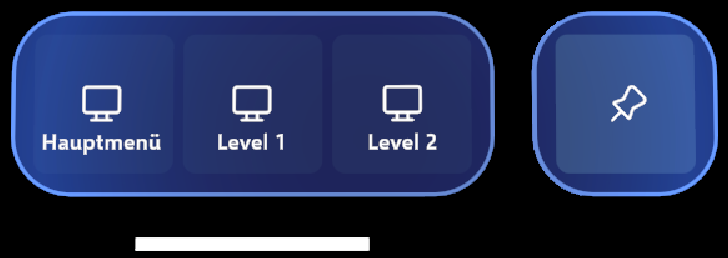
\includegraphics[width=0.8\textwidth]{images/menubarversion1.png}
    \caption{Darstellung des Erstentwurfes im Unity Editor}
    \label{fig:menübar}
\end{figure}

Die Abbildung \ref{fig:menübar} zeigt den ersten Entwurf des Menüs, das eine wichtige Schnittstelle für den Nutzer
darstellt, um zwischen verschiedenen Szenarien zu navigieren. Die Struktur des Menüs bleibt unabhängig vom jeweiligen
Spiellevel konstant, was zur Simplifizierung und Klarheit beiträgt. Die primären Schaltflächen auf der linken Seite
dienen der Initiation des Ladevorgangs für die verschiedenen Spielszenarien. Hervorzuheben ist der Pin-Button in
Kombination mit dem darunterliegenden weißen Balken. Diese beiden Funktionen gemeinsam ermöglichen es dem Benutzer,
das Menü an gewünschten Positionen zu verankern und bietet somit Flexibilität bei der Positionierung entsprechend
individueller Präferenzen. Ein solcher Einsatz ist von Vorteil, wenn externe Objekte die Nutzbarkeit des Menüs
beeinträchtigen könnten, wie zum Beispiel im Szenario des Platznehmens an einem Tisch, wo das Menü ungünstigerweise
mit dem Tisch kollidieren könnte und somit die Nutzererfahrung beeinträchtigt werden würde.

\subsubsection{Probleme beim Erstentwurf}
\subsubsection*{Problem 1 - Fehlende Dokumentation}
Das Hauptziel bei dem Konzept des Ersten Menüs, bestand darin, ein benutzerfreundliches Menü zu gestalten, das alle
erforderlichen Funktionen enthält und dennoch übersichtlich ist. Nach mehreren Iterationen und Tests mit Testpersonen,
die nicht mit dem Projekt vertraut waren, stellte sich heraus, dass der ursprüngliche Entwurf erhebliche Mängel bei der
Dokumentation und Erklärung der verschiedenen Anwendungsszenarien und ihrer jeweiligen Aufgaben aufweist. Es wurde
bemängelt, dass Benutzer lediglich zwischen den einzelnen Leveln wechseln können, ohne klare Informationen darüber zu
erhalten, worum es in den einzelnen Leveln geht und welche Aufgaben diese beinhalten.

Diese Feststellung verdeutlicht eine wesentliche Lücke in der Benutzerführung und -information innerhalb des Menüsystems.
Die unzureichende Dokumentation der Level und ihrer Ziele führt zu einer fehlenden Orientierung für die Benutzer und
kann sich negativ auf ihre Erfahrung auswirken. Das Menü sollte nicht nur als Navigationswerkzeug dienen, sondern auch
als Informationsquelle, die dem Benutzer eine klare Vorstellung über den Spielverlauf und die zu erreichenden Ziele vermittelt.

Die Identifizierung dieses Problems betont die Wichtigkeit einer umfassenden Benutzerforschung und -evaluation während
des Designprozesses. Dadurch wird sichergestellt, dass das entwickelte Benutzeroberflächensystem den Bedürfnissen und
Erwartungen der Zielgruppe entspricht. Eine zielgerichtete Überarbeitung des Menüs ist erforderlich, um die fehlende
Dokumentation der Anwendungsszenarien und ihrer Aufgaben zu adressieren und somit die Benutzererfahrung zu verbessern.

Bei Testdurchführungen ohne Entwickler aus dem Projektteam kam es wiederholt zu Unklarheiten bei den Benutzern,
insbesondere während des ersten Durchlaufs, bezüglich der zugewiesenen Aufgaben. Während der Nutzung der HoloLens-Anwendung
gab es vermehrt Anfragen seitens der Benutzer an das Projektteam aufgrund von Unklarheiten. Dies lässt vermuten, dass
die Anwesenheit von Entwicklern im Projektteam einen signifikanten Einfluss auf die Benutzererfahrung und Effektivität
der HoloLens-Anwendung hat.


\subsubsection*{Problem 2 - Falsche Wahl des Menütyps}
Während des Testprozesses stellte sich heraus, dass das Navigationsmenü oft eine Behinderung darstellte, insbesondere
für Entwickler, die Funktionen wiederholt testeten und Anwendungsszenarien neu luden. Das ständige Verschieben des Menüs
zur Seite erwies sich als zeitraubend und störte den Arbeitsfluss erheblich. Die ursprüngliche Intention, das
Navigationsmenü zur Erleichterung der Interaktion zwischen Benutzer und Spielumgebung einzuführen, erwies sich somit als kontraproduktiv.

Es ist wichtig, die Auswirkungen von Benutzeroberflächenelementen auf den Entwicklungsprozess zu berücksichtigen, um ein
reibungsloses Testen und Experimentieren zu gewährleisten. Eine effiziente und produktive Arbeitsweise des
Entwicklerteams hängt davon ab. Die Notwendigkeit einer kontinuierlichen Evaluation und Optimierung von
UI/UX-Komponenten während des gesamten Entwicklungszyklus wird durch dieses Problem verdeutlicht.

Dieses Problem verdeutlicht, dass der Erstentwurf und die ursprüngliche Konzeption hauptsächlich auf die Innovation und
Neuheit des Menüdesigns abzielten, anstatt den Fokus auf die funktionale Nützlichkeit zu legen. Der einfache und kompakte
Menütyp erwies sich als unzureichend, um eine umfassende und übersichtliche Dokumentation der Anwendungsszenarien zu
integrieren. Folglich war eine Migration zu einem alternativen Menüansatz erforderlich. Diese Beobachtung verdeutlicht
die Bedeutung einer ausgewogenen Gestaltung von Benutzeroberflächen in Mixed-Reality-Systemen. Es ist wichtig, dass
nicht nur ästhetische Innovationen verfolgt werden, sondern auch die tatsächliche Benutzererfahrung und -effizienz in
Betracht gezogen wird. Die Reflexion über diesen Prozess bietet Einsichten in die iterative Entwicklung von
Benutzerschnittstellen und die Anpassung an die Anforderungen und Rückmeldungen der Benutzer.

\subsection{Finalversion des Menüs}
Die endgültige Version des Menüs wurde entwickelt, um die Mängel des ursprünglichen Entwurfs anzugehen und idealerweise
vollständig zu beheben. Dieses neue Konzept wurde durch eine umfassende Analyse populärer AR/VR-Spiele geleitet, um die
Gründe für die verbesserte Benutzererfahrung in diesen Kontexten zu untersuchen. Dabei wurden spezifische Merkmale und
Designentscheidungen identifiziert, die einen signifikanten Einfluss auf die Zufriedenheit der Anwender haben.

Basierend auf vorangegangenen Recherchen wurde entschieden, das neue Menü in zwei klar definierte Bereiche zu unterteilen.
Dies gewährleistet eine deutliche Unterscheidung des Hauptmenüs sowie eine klare Orientierung bezüglich der Navigation.
Insbesondere innerhalb der Anwendungsszenarien wurde ein minimalistisches und unaufdringliches Menü implementiert, um
den Fokus der Benutzer uneingeschränkt auf die auszuführenden Tätigkeiten zu lenken. Diese Designstrategie hat zum Ziel,
die kognitive Belastung der Benutzer zu reduzieren und eine nahtlose Integration der Menüfunktionalitäten in den jeweiligen
Nutzungskontext zu ermöglichen.

Das Ergebnis ist ein ansprechendes und benutzerorientiertes Menükonzept, das die Gesamterfahrung des Spiels verbessert
und den Erwartungen der Zielgruppe gerecht wird.

\subsubsection{Finalversion Menü - Hauptmenü}
Auf dieser Grundlage wurde das Design des Menüsystems vollständig überarbeitet, wobei der erste Schritt schonmal die
vollständige Entfernung der Idee des Nahmenüs beinhaltet.

Anstelle des Nahmenüs wurden vorgefertigte Objekte in das Hauptmenü integriert, welche zuvor mit Blender modelliert wurden.
Die Entscheidung, vorgefertigte Objekte aus Blender zu importieren, bietet eine breite Palette an Gestaltungsmöglichkeiten
und ermöglicht es, das Menü visuell ansprechend und einladend zu gestalten. Außerdem trägt die Integration dieser Objekte
dazu bei, das Menü intuitiver und zugänglicher zu machen, indem sie dem Benutzer klare Anhaltspunkte und Handlungsmöglichkeiten bieten.

\begin{figure}[H]
    \centering
    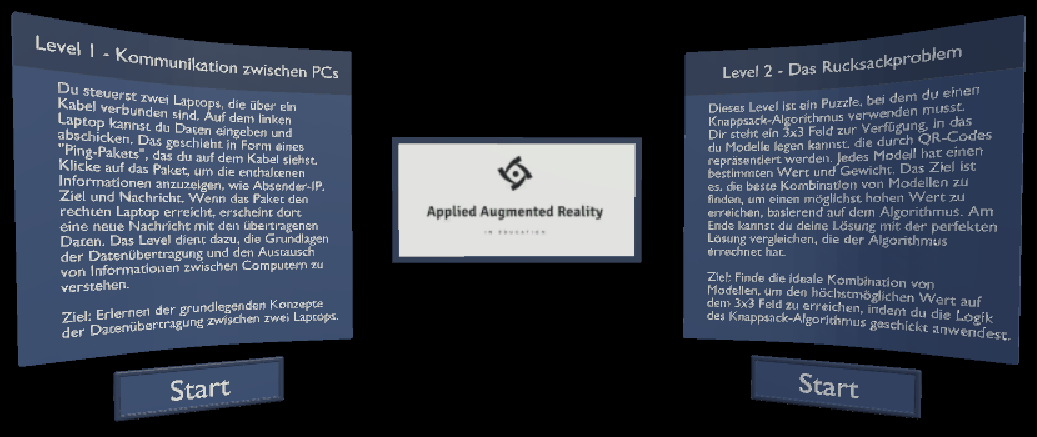
\includegraphics[width=1\textwidth]{images/menuversion2.png}
    \caption{Darstellung des Finalen Menüs im Unity Editor}
    \label{fig:menuversion2}
\end{figure}

Die in der Abbildung \ref{fig:menuversion2} dargestellten Objekte bestehen aus zwei separaten Tafeln, die durch unser
Diplomarbeitslogo voneinander getrennt sind. Jede Tafel enthält den Titel des Anwendungsszenarios sowie einen vorgefertigten
Startbutton.  In Unity wurde ein unsichtbarer, aber dennoch klickbarer Button mit exakt denselben Dimensionen wie das
Modell des Startbuttons an der entsprechenden Stelle platziert. Das Skript \textit{SceneChange.cs}, welches für die
Szenenwechsel-Funktionalität verantwortlich ist, ist diesem Button angehängt.

\begin{figure}[H]
    \centering
    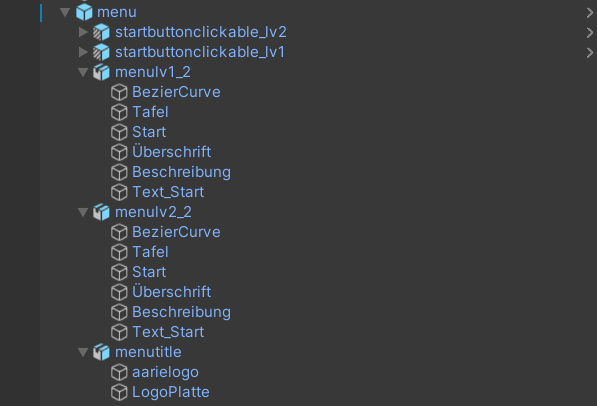
\includegraphics[width=0.8\textwidth]{images/hierarchiemenuunity.png}
    \caption{Darstellung der Hierarchie des finalen Menüs im Unity Editor}
    \label{fig:hierarchiemenuunity}
\end{figure}

In der Abbildung \ref{fig:hierarchiemenuunity} ist die Hierarchie des Hauptmenüs im Unity Editor zu sehen. Dem
Prefab \textbf{menu} sind dabei 5 einzelne Objekte zugewiesen. Die Prefabs \textbf{startbuttonclickable\_lv1/2} sind die
in Unity erstellen unsichtbaren Button die dafür zuständig sind den vormodellierten Buttons eine Funktion zu geben. Darunter
zu sehen sind die 3 verschiedenen Assets welche aus blender importiert wurden. Diese bestehen jeweils aus den verschiedenen
Einzelteilen, welche in Unity als Gameobjects dargestellt werden. Die \textbf{BezierCurve} ist eine spezielle Art von Kurve
welche in Blender für die leichte Wölbung der Tafeln genutzt wurde.

\subsubsection{Finalversion Menü - Anwendungsszenario}
Im Gegensatz zum Erstentwurf, der ein einheitliches Menü für alle Anwendungsszenarien vorsah, weist diese Version eine
Differenzierung auf. Die Entscheidung, das Menü innerhalb der einzelnen Szenarien anzupassen, wurde getroffen, um die volle
Aufmerksamkeit des Benutzers auf das jeweilige Level und die darin ausgeführten Aktivitäten zu lenken. Aus diesem Grund
wurde ebenfalls das Nahmenü aus den Szenarien entfernt und durch ein simples Handmenü ersetzt.

\begin{figure}[H]
    \centering
    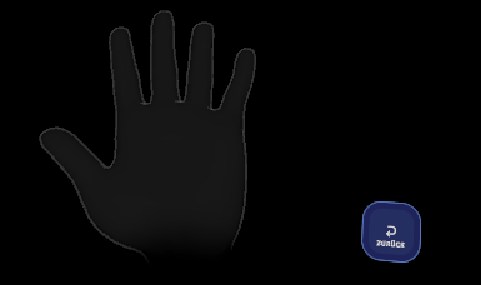
\includegraphics[width=0.8\textwidth]{images/backbutton.png}
    \caption{Darstellung des Finalen Menüs im Anwendungsszenario im Unity Editor}
    \label{fig:backbutton}
\end{figure}

Wie in der Abbildung \ref{fig:backbutton} gezeigt, besteht dieses Menü ausschließlich aus einem Zurück-Knopf, der den
Benutzer zum Hauptmenü zurückführt. Das Handmenü wurde so konzipiert, dass es nur dann sichtbar ist, wenn der Benutzer
es benötigt oder aktivieren möchte.  Der Zurückknopf wird erst sichtbar, wenn der Benutzer seine linke Hand umdreht und
auf die Handfläche schaut.

Diese Funktionalität hat zum Ziel, die Benutzerinteraktion intuitiver und kontextbezogener zu gestalten. Hierfür wird
Bewegungserkennung und Blickrichtungserkennung genutzt, um das Handmenü nur dann einzublenden, wenn der Benutzer aktiv
nach einem Navigationsmittel sucht. Dadurch wird visuelle Ablenkung minimiert und die Benutzererfahrung optimiert, indem
nur relevante Informationen und Interaktionselemente präsentiert werden, wenn sie benötigt werden.

\subsubsection{Setzen des Menüs}
Bei dem Erstentwurf gab es keine Probleme beim Wechseln zwischen den Szenen beziehungsweise dem Laden in das Hauptmenü,
jedoch muss man in der neuen Version darauf achten das Menü richtig zu setzen. Dafür muss man die Modelle im richtigen
moment und an der richtigen Stelle in der richtige Szene selbstständig instanzieren, deshalb wurde extra für diesen Fall
das \textit{MenuSpawn.cs} Skript geschrieben.

\begin{lstlisting}[style=csharp, caption=Menüinstanzierung bei Neuladen., label=code:spawnmenu]
using System.Collections;
using System.Collections.Generic;
using UnityEngine;

public class SpawnPrefab : MonoBehaviour
{
    public GameObject menu;

    void Start()
    {
        SpawnPrefabMenu();
    }

    void SpawnPrefabMenu()
    {
        Vector3 cameraPosition = Camera.main.transform.position;
        Vector3 spawnPosition = new Vector3(cameraPosition.x, cameraPosition.y, cameraPosition.z + 1f);
        Instantiate(menu, spawnPosition, Quaternion.identity);
        menu.SetActive(true);
    }
}
\end{lstlisting}

Beim Start der Anwendung wird die Methode \textit{SpawnPrefabMenu()} ausgeführt. Diese Methode ist für die Positionierung
des Menüs verantwortlich. Die im Codeabschnitt \ref{code:spawnmenu} ersichtlichen Positionsvektoren sind einerseits dafür
zuständig, die aktuelle Kameraposition zu ermitteln, aber auch eine neue Spawnposition zu setzen, die um 1 auf der z-Achse
versetzt ist, so dass das Menü vor dem Benutzer erscheint. Der \textit{Instantiate} ist dafür verantwortlich, dass das Menü
an der jeweiligen Spawnposition gesetzt wird. Anschließend wird das zuvor versteckte Menü mit \textit{menu.SetActive(true)}
aktiviert, so dass der Benutzer es sehen und mit ihm interagieren kann.

%\subsection{Vergleich der Menüentwürfe} (vielleicht mach ich das noch)
\subsection{Laden der Level}
Um den Buttons eine Funktion zuzuweisen, wird ein Skript benötigt, das aktiviert wird, sobald ein Button gedrückt wird.
Im vorliegenden Fall ist das Skript \textit{SceneChange.cs} für den Wechsel zwischen den verschiedenen Anwendungsszenarien verantwortlich.
Wenn einer der Buttons im Hauptmenü gedrückt wird, wird dieses Skript ausgeführt. Die Spielszene wird im Unity Inspector
festgelegt. Der Code greift auf die Variable zu, die den Namen der Szene enthält, wie sie zuvor im Inspector benannt wurde.

\begin{figure}[H]
    \centering
    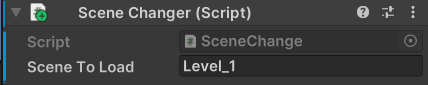
\includegraphics[width=0.6\textwidth]{images/sceneToLoad.png}
    \caption{Darstellung der SceneToLoad Variable, anhand des Level1 Buttons.}
    \label{fig:scenetoload}
\end{figure}

Für den linken Button im Hauptmenü ist beispielsweise die Spielszene \textit{Level1} vorgesehen, während für den rechten
Button die Szene \textit{Level2} zugewiesen ist. Durch diese Konfiguration im Inspector wird die Flexibilität gewährleistet,
Szenen dynamisch anzupassen, ohne dass Änderungen am eigentlichen Skript vorgenommen werden müssen. Dies ermöglicht eine
effiziente Verwaltung und Anpassung der Spielinhalte während des Entwicklungsprozesses.

\begin{lstlisting}[style=csharp, caption=Auf Knopfdruck Szene wechseln., label=code:scenechange]
using UnityEngine;
using UnityEngine.SceneManagement;

public class SceneChanger : MonoBehaviour
{
    public string sceneToLoad;

    public void ChangeScene()
    {
        if(SceneManager.GetActiveScene().name != sceneToLoad)
        {
            PlayerPrefs.DeleteAll();
            SceneManager.LoadScene(sceneToLoad, LoadSceneMode.Single);
        }
    }
}
\end{lstlisting}

Das vorliegende Skript hat eine vergleichsweise einfache Struktur. Die Variable \textbf{public string sceneToLoad} dient
als Empfänger für den Namen der zu ladenden Szene, welcher im Unity-Inspector individuell für jede Szene festgelegt werden
kann. Um den Szenenwechsel zu initiieren, wird die Methode \textbf{ChangeScene()} aufgerufen. Zunächst wird in dieser
Methode geprüft, ob die aktive Szene, die durch \textbf{SceneManager.GetActiveScene()} ermittelt wird, mit der zu ladenden
Szene übereinstimmt. Falls dies nicht der Fall ist, werden alle gespeicherten PlayerPrefabs mittels
\textbf{PlayerPrefs.DeleteAll()} gelöscht. Dieser Schritt ist von entscheidender Bedeutung, um potenzielle Komplikationen
im Zusammenhang mit dem HoloLens-Cache während des Szenenwechsels zu vermeiden.

Nachdem die Prefabs bereinigt wurden, wird die definierte Szene mit der Methode \textbf{SceneManager.LoadScene()}
geladen. Dabei wird die Ladeoption \textbf{LoadSceneMode.Single} verwendet, um sicherzustellen, dass nur die angegebene
Szene aktiv geladen wird und keine anderen Szenen im Hintergrund verbleiben. Diese präzise Steuerung des Ladevorgangs
zielt darauf ab, die Performance und Stabilität der Anwendung auf der HoloLens-Plattform zu optimieren und potenzielle
Konflikte zwischen Szeneninhalten zu vermeiden.

\subsection{UI/UX}
Die Gestaltung der Benutzeroberfläche und die damit verbundene Benutzererfahrung sind wesentliche Aspekte bei der
Konzeption und Entwicklung von Software. Eine bewährte Strategie besteht darin, sich an populären und gleichgerichteten
Anwendungen zu orientieren, insbesondere im Bereich der Augmented- oder Virtual Reality. Es wird darauf geachtet, komplexe
und verwirrende Menüstrukturen zu vermeiden und eine konsistente Farbpalette über die gesamte Benutzeroberfläche hinweg zu verwenden.

Diese Herangehensweise basiert auf der Erkenntnis, dass erfolgreiche Anwendungen in ähnlichen Domänen oft bewährte
Designprinzipien und Interaktionsmuster aufweisen, die sich positiv auf die Benutzerakzeptanz und -zufriedenheit auswirken
können. Durch die Anpassung an gängige Standards und Trends in der Branche kann das Risiko von Benutzerirritationen
und -ablehnungen minimiert werden. Gleichzeitig wird eine vertraute und angenehme Benutzererfahrung gefördert.

Es ist wichtig zu betonen, dass eine solche Inspiration von bestehenden Anwendungen nicht als direkte Kopie verstanden
werden sollte, sondern vielmehr als Quelle für Anregungen und bewährte Praktiken, die in einem eigenständigen und angepassten
Kontext implementiert werden können. Auf diese Weise kann die Effektivität und Attraktivität der Benutzeroberfläche
optimiert werden, um die Bedürfnisse und Erwartungen der Zielgruppe bestmöglich zu erfüllen.



\section{Ping Scenario} \marginpar{\small(\rightarrow) Schoditsch}
In diesem Szenario wird das IT-Grundprinzip des Ping illustriert. Zwei PCs sind in einer realen Umgebung durch ein
rotes Kabel miteinander verbunden, wobei auf jedem PC dieselbe Website geöffnet ist. Der Benutzer trägt eine HoloLens 2
und erhält die Aufforderung, das rote Kabel zu betrachten. Nach einem Countdown wird ein Foto der Umgebung aufgenommen
und anschließend verarbeitet. Dabei werden Raycasts eingesetzt, um die exakte Position des roten Kabels in der
physischen Welt zu bestimmen. Sobald die Position des Kabels erkannt wurde, kann der Benutzer über die Website auf den
beiden PCs eine Nachricht senden. Diese Nachricht wird dann in Form eines Pakets für den Hololens 2 benutzer
visualisier. Der Benutzer hat außerdem die Möglichkeit, auf das Paket zu drücken, um die Informationen wie Absender und
Nachricht einzusehen.

\subsection{Aufbau von Ping Scenario}
In diesen Abschnitt wird beschrieben wie die Unity Scene aufgebaut ist und
was die aufgabe der einzelnen GameObjects ist.

\begin{figure}[h]
    \centering
    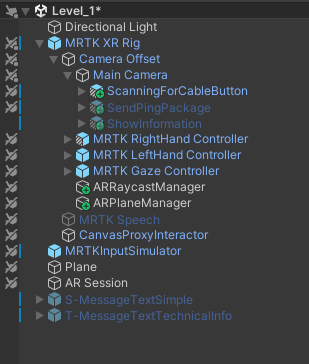
\includegraphics[scale=1]{images/Level1Hierarchy.png}
    \caption{Hierarchie des Ping Levels im Unity Editor.}
    \label{fig:level1_hierarchy}
\end{figure}
\begin{itemize}
    \item \textbf{Level-1:} Die Scene in der alle Unity-Objekte enthalten sind.
    \item \textbf{UserInfo:} Gameobject welches den Hololens Benutzer einen Countdown angibt und von welchem aus
    daraufhin alle anderen Scripte ausgeführt werden.
    \item \textbf{LoadingCircle:} Während ladezeiten wird dieses Gameobject angezeigt um den Benutzer zu infomieren das
    dass Programm berechnungen ausführt. Das Objekt beinhalted ein Canvas wo das User Interface enthalten ist.
    \item \textbf{Plane:} Ist ein Script GameObject welches den code ausführt. Kann auch zum debug genutzt werden da es
    die erkannten roten Pixel visuell darstellt
    \item \textbf{InfoObjectS:} Beinhaltet den Simplen Text welcher angezeigt wird sobald ShowInformation betätigt wird.
    \item \textbf{InfoOjectT:} Gleich wie InfoObjectS nur mit den technischen informationen eines Ping-Pakets.
    \item \textbf{S-MessageTextTechnicalInfo:} Gleich wie S-MessageTextSimple nur mit den technischen informationen
     eines Ping-Pakets.
\end{itemize}

\subsection{Kabel erkennung}
\subsubsection{Foto der umgebung schießen}
Zu Beginn der Szene wird der Benutzer aufgefordert, auf das rote Kabel zu schauen. Anschließend wird ein Countdown
gestartet, während dessen ein Foto mit Hilfe der PhotoCapture-Klasse aufgenommen wird.

\subsubsection{Foto verarbeitung}
Nachdem ein Foto aufgenommen wurde, erfolgt die Datenverarbeitung mittels einer Texture2D-Klasse innerhalb des
Unity-Job-Systems in paralleler Ausführung. Jeder Thread des Systems ist dafür zuständig, eine festgelegte Anzahl von
Pixeln im Bild zu überprüfen, um festzustellen, ob diese die Eigenschaft Rot aufweisen. Die Ergebnisse dieser
Überprüfung werden in einem zweidimensionalen Boolean-Array gespeichert, wobei die x- und y-Koordinaten jeweils einer
Dimension zugeordnet sind. Jeder Pixel im Array wird entsprechend seines Farbzustands mit dem booleschen Wert
\textit{true} gekennzeichnet, falls er rot ist, andernfalls wird ihm der Wert \textit{false} zugewiesen. Dieser Prozess
wird durch das Job-System ausgeführt, wobei jeder einzelne Job die anliegende Operationen durchführt:

\begin{lstlisting}[style=csharp, caption={Rote pixel suche}, label=code:PixelJob]
    struct PixelJob : IJobParallelFor
    {
        public NativeArray<Color> pixels;
        public NativeArray<Vector2> redPixelPositions;
        public int textureWidth;
        public int batchSize;

        public void Execute(int batchIndex)
        {
            int startPixelIndex = batchIndex * batchSize;
            int endPixelIndex = Mathf.Min((batchIndex + 1)
            * batchSize, pixels.Length);

            for (int pixelIndex = startPixelIndex;
            pixelIndex < endPixelIndex; pixelIndex++)
            {
                int x = pixelIndex % textureWidth;
                int y = pixelIndex / textureWidth;

                if (pixels[pixelIndex].r > 0.7f &&
                pixels[pixelIndex].g < 0.5f && pixels[pixelIndex].b < 0.5f)
                {
                    pixels[pixelIndex] = Color.red;
                    redPixelPositions[pixelIndex] = new Vector2Int(x, y);
                }
                else
                {
                    pixels[pixelIndex] = Color.black;
                }
            }
        }
    }
\end{lstlisting}
\begin{itemize}
    \item \textbf{NativeArray:} bietet verbesserte Leistung da sie direkt auf native Speicherbereiche zugreifen können,
    was besonders wichtig ist, wenn große Datenmengen verarbeitet werden müssen und die Ausführung parallelisiert
    werden soll.
    \item \textbf{startPixelIndex:} nachdem jeder Arbeiter Thread seine eigenen batches besitz muss der Index für diese
    berechnet werde.
\end{itemize}


\subsubsection{Kabel finden}
Da das Programm nur die Positionen der roten Pixel identifiziert und es unsicher ist, ob sie zu einem Kabel gehören,
wird eine Methode angewendet, um die längste zusammenhängende Reihe von roten Pixeln zu ermitteln. Es kann auch dazu
kommen das rote Pixel nicht erkannt werden welche zum Roten Kabel gehören. Aus diesem Grund wird ein Toleranzbereich
festgelegt. Es wird geschaut ob in einen bestimmten bereich ein rote Pixel exestieren von welchen aus dann weiter
geschaut wird. Dadurch wird eine präzisere Erkennung und Zuordnung von relevanten roten Pixeln im Kontext des zu
identifizierenden Kabels ermöglicht. Die methodische Vorgehensweise zur Berechnung gestaltet sich wie folgt:

\begin{lstlisting}[style=csharp, caption={Kabel suche}, label=code:SearchForRedPixels]
ist<Vector2> SearchForRedPixels(int startX, int startY)
    {
        List<Vector2> currentLine = new List<Vector2>();´
        bool hasFound = false;
        int foundX = startX, foundY = startY;
        int heightY = redPixels.GetLength(1);
        int withX = redPixels.GetLength(0);

        do
        {
            hasFound = false;
            redPixels[foundX, foundY] = false;
            currentLine.Add(new Vector2(foundX, foundY));

            for (int i = 1; i < 25 && foundX + i < withX; i++)
            {

                if (redPixels[foundX + i, foundY])
                {
                    foundX = foundX + i;
                    hasFound = true;
                }
            }

            for (int i = 1; i < 10 && !hasFound && foundY - i > 0; i++)
            {
                hasFound = redPixels[foundX, foundY - i];

                if (hasFound)
                {
                    foundY = foundY - i;
                }
            }

            for (int i = 1; i < 10 && !hasFound && foundY + i < heightY; i++)
            {
                hasFound = redPixels[foundX, foundY + i];

                if (hasFound)
                {
                    foundY = foundY + i;
                }
            }
        } while (hasFound);
        return currentLine;
    }
\end{lstlisting}
Wenn wir das Koordinatensystem von einem Standpunkt aus betrachten, an dem die positive x-Achse nach rechts zeigt, die
negative x-Achse nach links zeigt, die positive y-Achse nach oben zeigt und die negative y-Achse nach unten zeigt, dann
kann man sagen, dass der Code nach oben, rechts und unten schaut.

\subsubsection{Entfernung messen}
Da man noch die z-Achse, also die Tiefe, zu ermitteln, um das visuelle Paket angemessen zu platzieren, werden
im späteren Verlauf RayCasts verwendet. Aufgrund der Ressourcenintensität, die mit dem Versenden eines Raycasts
für jede Position verbunden wäre, um die z-Achse für jede Koordinate zu erhalten, wird eine Optimierung angestrebt.
Zur Verbesserung der Effizienz werden die wichtigsten Positionen berechnet. Diese wichtigen Punkte sind der
anfangspunkt des Kabels (am ersten PC), der mittelpunkt des Kabels, das endpunkt des Kabels (am zweiten PC), sowie 10
andere punkte welche auf den Kabel verteilt sind.

\subsubsection*{Definition eines Rays} % Quelle: https://docs.unity3d.com/ScriptReference/Physics.Raycast.html
Ein Ray ist ein abstraktes Konzept in der Computergrafik und Physiksimulation, das einen unendlich langen, geraden
Strahl repräsentiert. Dieser Strahl wird durch einen Ausgangspunkt definiert, der üblicherweise als \textit{Ursprung}
bezeichnet wird. Im Kontext von dreidimensionalen Szenen und Visualisierungen entspricht der Ursprung oft der Position
einer \textit{virtuellen Kamera} oder eines \textit{Blickpunkts}.

Der Ray erstreckt sich dann in eine bestimmte Richtung, die durch Vektoren definiert wird. Diese Richtung kann durch
verschiedene Methoden festgelegt werden, abhängig von der Anwendung, in der der Ray verwendet wird. Im Falle der
Bildschirmkoordinaten kann die Richtung beispielsweise durch  Blick des Benutzers bestimmt werden.

In der Praxis wird der Ray häufig dazu verwendet, um \textit{Kollisionen mit Objekten in einer Szene zu erkennen} oder
\textit{um Lichtstrahlen für die Beleuchtungsberechnung zu simulieren}. Durch das Schießen eines Rays in eine Szene und
das Überprüfen auf \textit{Kollisionen} mit den vorhandenen Objekten kann festgestellt werden, ob der Ray ein Objekt
trifft und wenn ja, an welcher \textit{Stelle} und unter welchem \textit{Winkel}.\\

\subsubsection{Bewegung des Packetes}
Nach der Bestimmung der kritischen Positionen mittels Raycast hat der Benutzer die Möglichkeit, über die Website eine
Nachricht zu übermitteln. Die Übermittlung dieser Nachricht löst ein entsprechendes Ereignis aus, das zur
Initialisierung und zum absenden des Datenpakets führt.

\subsection{Starten und verwenden der Webseite} \marginpar{\small\(\rightarrow\) HAYLAZ}
TODO

% Keine Ahnung was Jonas hier macht aber ich füg mal mein Stuff ein hehe
\subsection{Frontend der Webseite} \marginpar{\small\(\rightarrow\) LAMPEL}
In diesem Abschnitt wird die Struktur und Entwicklung des Frontends der Webseite erläutert. Besonderes Augenmerk wird
auf die zugrundeliegenden Entscheidungen bezüglich der Programmiersprachen sowie des Designprozesses gelegt.

Nach mehreren Entwicklungszyklen im ersten Anwendungsszenario wurde entschieden, eine Webseite in das Projekt zu
integrieren. Die Funktionalität der Webseite sollte nahtlos in das Szenario integriert werden. Hierzu können Nachrichten
und Absender direkt auf der Webseite eingetragen werden, um sie anschließend in die HoloLens-Applikation zu übertragen.

\subsubsection{Designprozess}
Beim Entwurf einer Webseite ist es essentiell, vor der eigentlichen Umsetzung die Farbpalette und das generelle Aussehen
der Seite zu konzipieren. Da der Fokus auf der Anwendung auf der HoloLens liegt, wurde bewusst darauf geachtet, der
Webseite nicht zu viel Aufmerksamkeit zu schenken. Sie sollte lediglich die grundlegenden Funktionen erfüllen, ohne dabei
komplex zu sein. Aus diesem Grund ist die Webseite simpel gestaltet und verfügt über wenige Eingabefelder und wenig Text.

\subsubsection*{Webseitenprototyp}
Der Prototyp der Webseite, wie in Abbildung \ref{fig:protfrontend} dargestellt, gibt einen Überblick über das
Frontend-Design. Das Zahnrad links oben öffnet ein Fenster, in dem die IP-Adresse der HoloLens eingegeben werden kann,
um Nachrichten korrekt zu versenden. Auf der Hauptseite gibt es Eingabefelder für Benutzername und Nachricht. Der zeitlich
sortierte Nachrichtenverlauf wird am rechten Rand angezeigt.

\begin{figure}[H]
    \centering
    \fbox{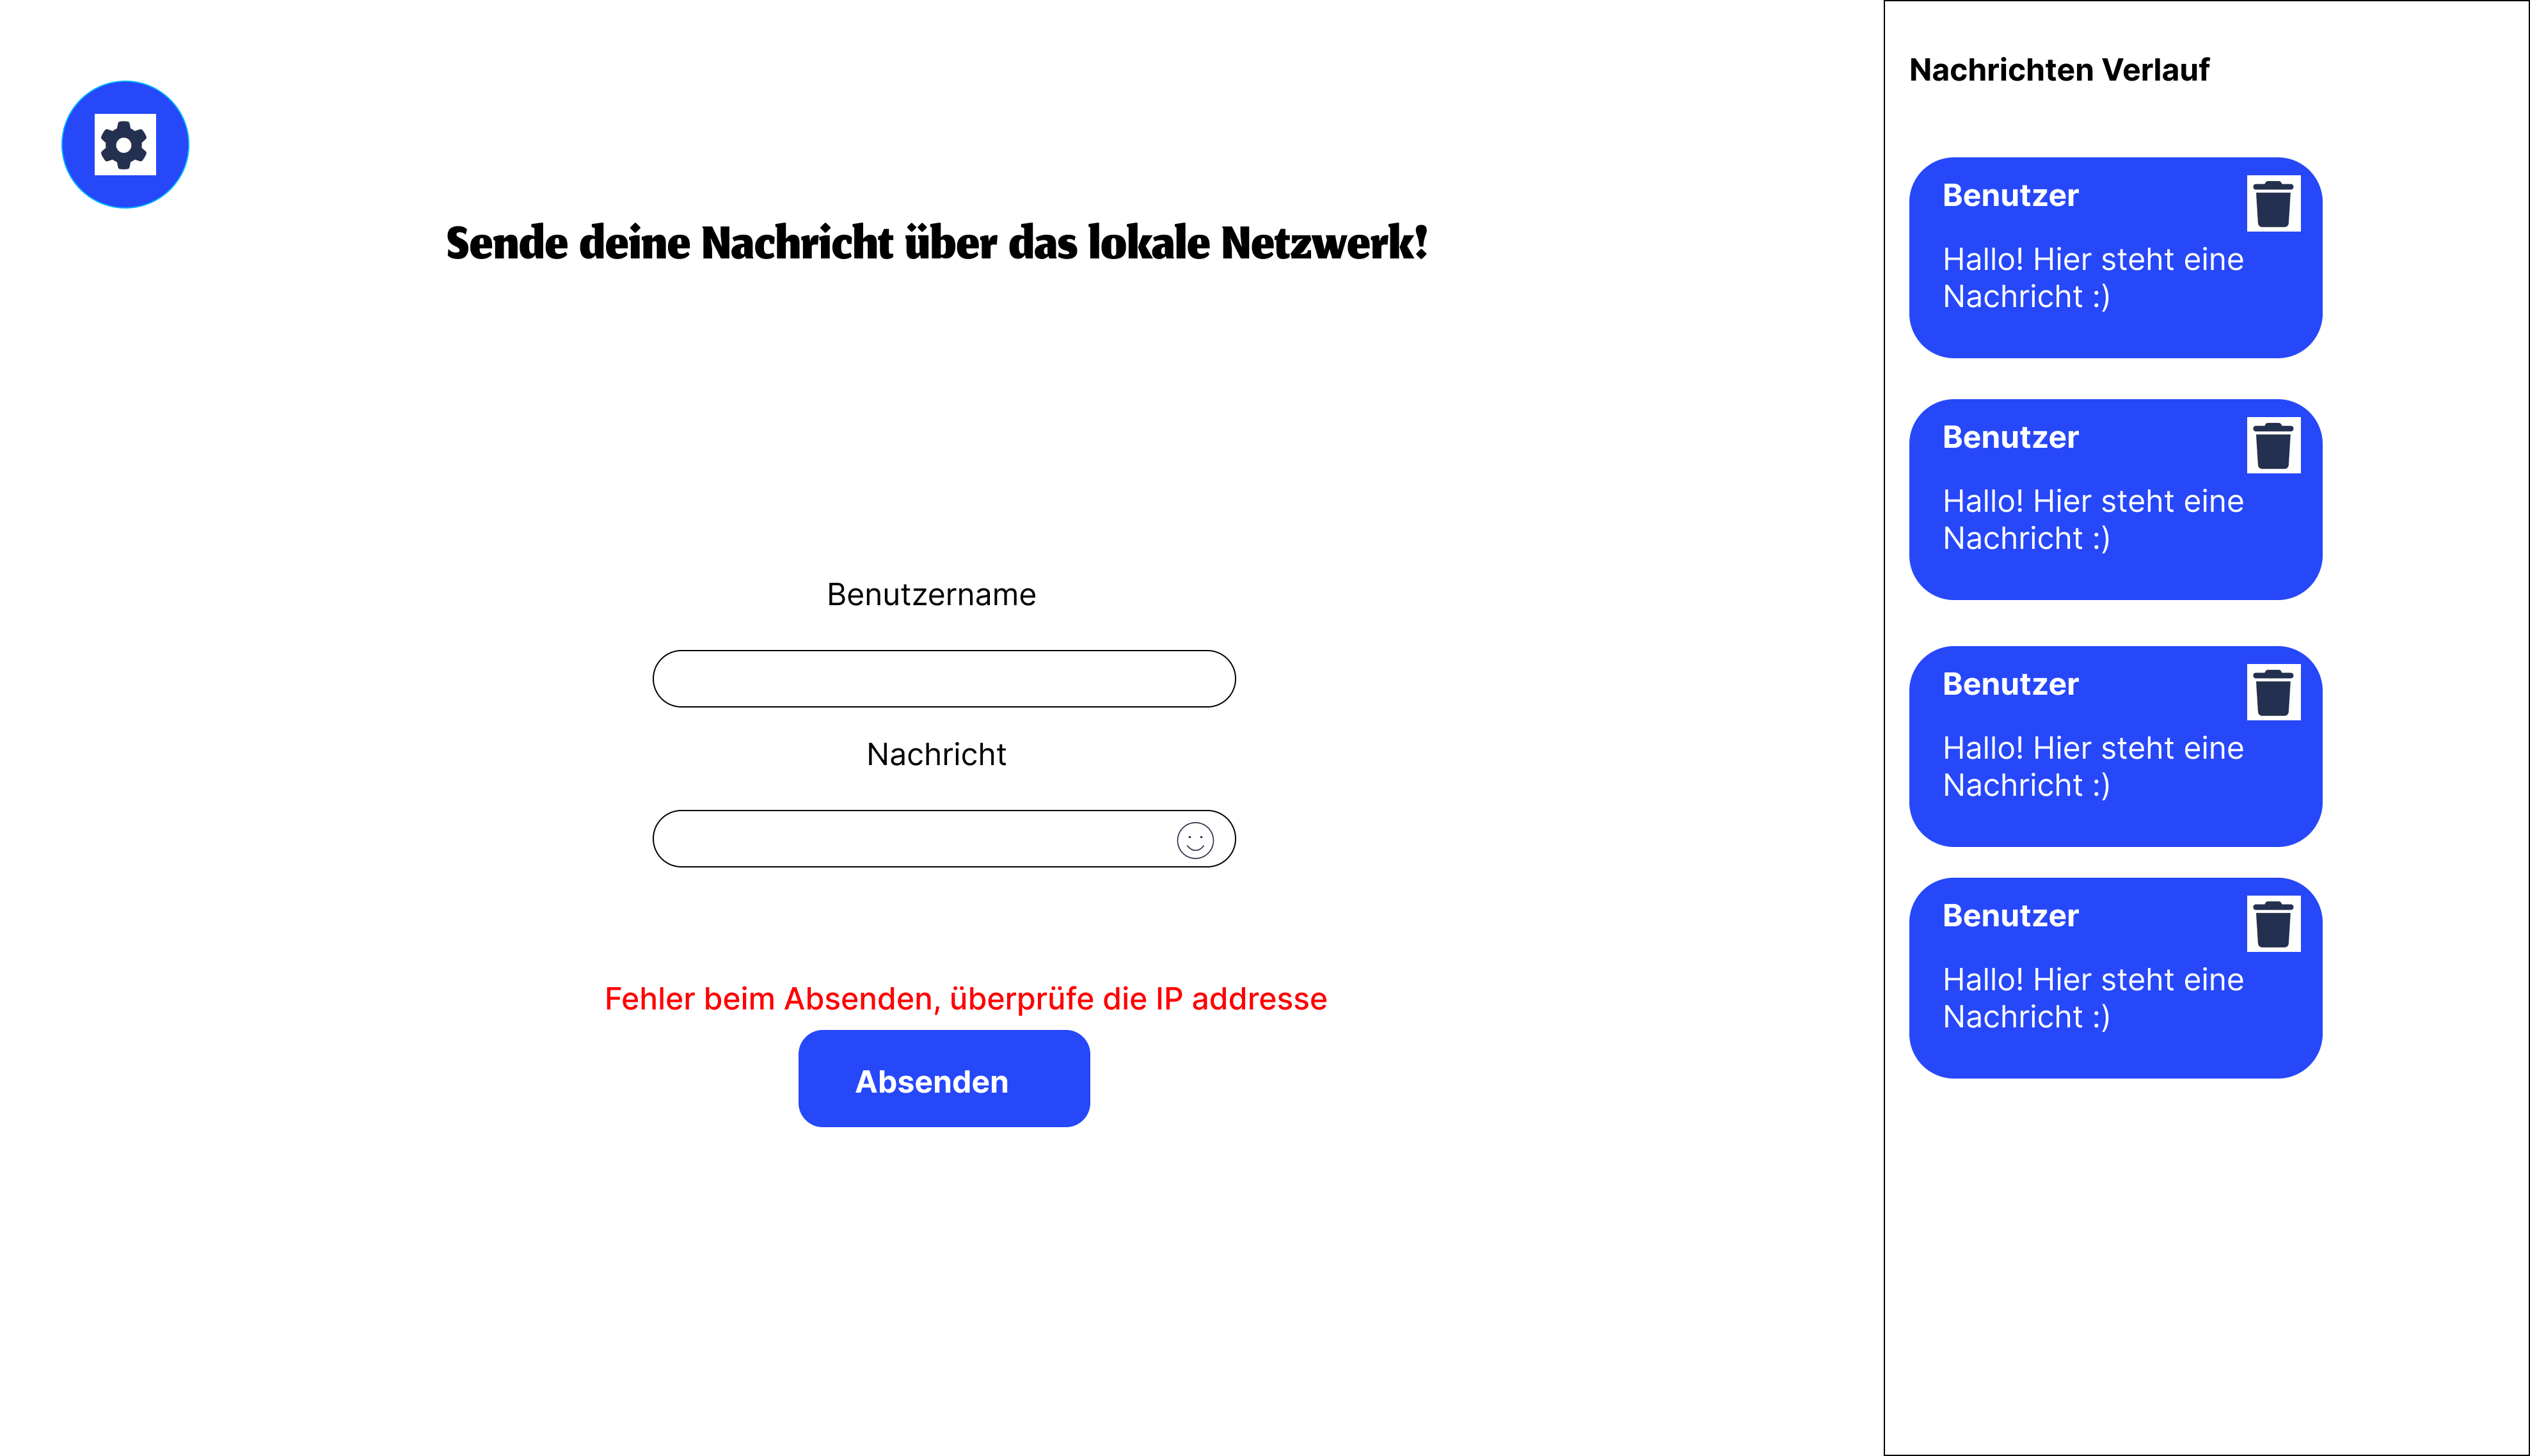
\includegraphics[width=1\textwidth]{images/prototypefrontend.png}}
    \caption{Prototypische Darstellung der Webseitenansicht aus Benutzersicht}
    \label{fig:protfrontend}
\end{figure}

\subsubsection*{Ausprogrammierte Webseite}
Die endgültige Version der Webseite, wie in Abbildung \ref{fig:frontend} gezeigt, enthält alle gewünschten Funktionen.
Die Farbpalette orientiert sich stark am Hauptmenü und den Standardfarben der HoloLens. Es werden verschiedene Blautöne
verwendet, um eine konsistente und benutzerfreundliche Benutzererfahrung zu gewährleisten.

\begin{figure}[H]
    \centering
    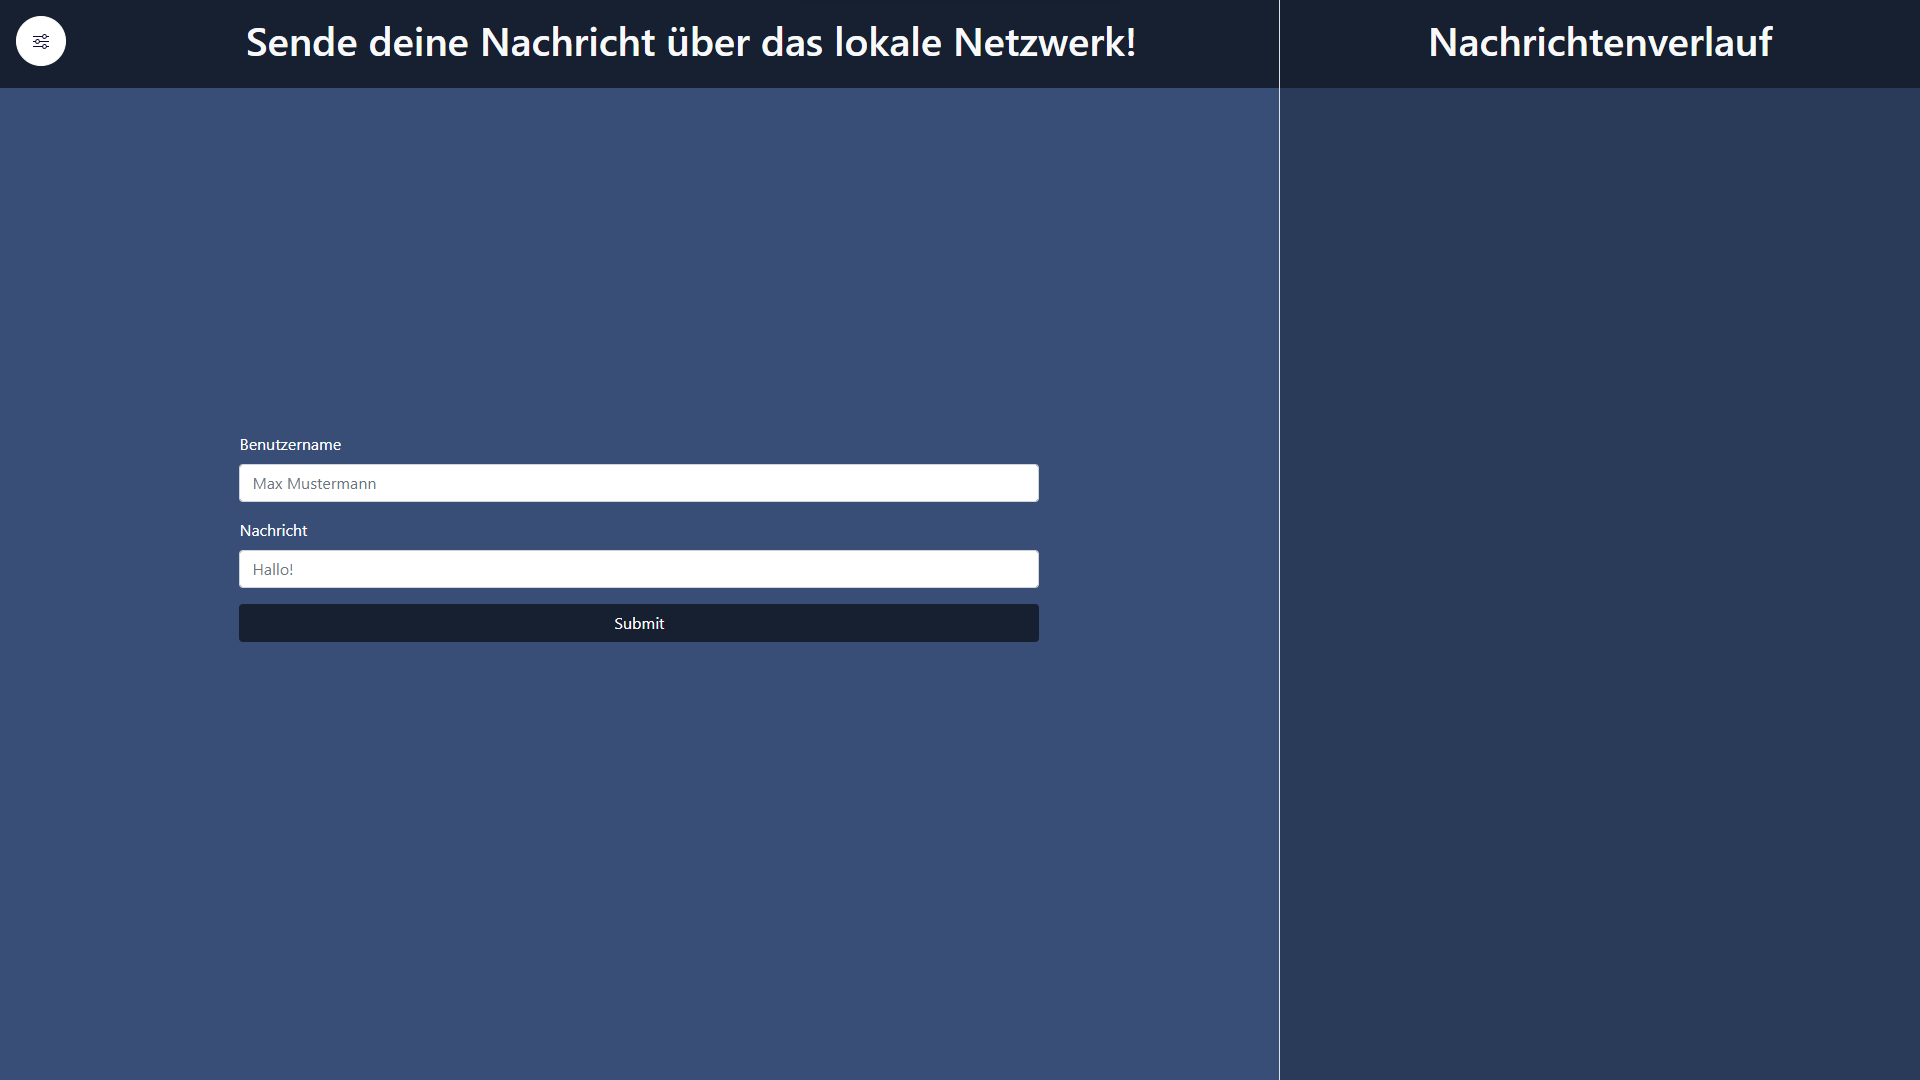
\includegraphics[width=1\textwidth]{images/frontend.png}
    \caption{Darstellung der fertigen Webseitenansicht aus Benutzersicht}
    \label{fig:frontend}
\end{figure}

Die Umsetzung des Designs hat zum Ziel, Verwirrungen zu vermeiden und eine nahtlose Integration der Webseite in das
Gesamtsystem zu gewährleisten.

\subsubsection{Verwendete Programmiersprachen}
Für die Entwicklung der Webseite wurden hauptsächlich die Programmiersprachen HTML, CSS und JavaScript verwendet. Zur
Verbesserung des Designs und der Benutzererfahrung wurde außerdem das Framework Bootstrap eingesetzt.

\subsubsection*{HTML (Hypertext Markup Language)}
HTML ist die grundlegende Struktursprache des World Wide Web. Es ermöglicht die Erstellung von Webseiten durch die
Definition von Strukturelementen wie Überschriften, Absätzen, Listen und Links. HTML verwendet Tags, um den Browsern
mitzuteilen, wie die Inhalte einer Webseite strukturiert und präsentiert werden sollen. \footnote{Mozilla Developer Network \cite{HTML}}

\subsubsection*{CSS (Cascading Style Sheets)}
CSS ist eine Stylesheet-Sprache, die verwendet wird, um das Aussehen und die Formatierung von HTML-Dokumenten zu steuern.
Es ermöglicht die Definition von Farben, Schriftarten, Layouts und anderen visuellen Eigenschaften einer Webseite. \footnote{Mozilla Developer Network \cite{CSS}}

CSS funktioniert durch das Zuweisen von Regeln und Stilen zu HTML-Elementen. Diese Regeln können in einer externen
CSS-Datei definiert oder direkt im HTML-Dokument eingebettet werden.

\subsubsection*{JavaScript}
JavaScript ist eine dynamische Programmiersprache, die hauptsächlich für die clientseitige Entwicklung von Webanwendungen
verwendet wird. Sie ermöglicht die Interaktion mit dem Benutzer, das Ändern von Inhalten in Echtzeit und die Steuerung
des Verhaltens einer Webseite. \footnote{Mozilla Developer Network \cite{Javascript}}

JavaScript verbessert die Funktionalität einer Webseite, indem es auf Benutzerinteraktionen reagiert, Formulare validiert,
Animationen erstellt und vieles mehr.

\subsubsection*{Integration von Bootstrap}
Bootstrap ist ein Open-Source-Framework für die Frontend-Entwicklung von Webseiten und Webanwendungen. Es bietet
vorgefertigte HTML- und CSS-Vorlagen für Typografie, Formulare, Buttons, Navigation und andere UI-Komponenten. \footnote{Bootstrap Dokumentation \cite{Bootstrap}}

Bootstrap erleichtert die Erstellung responsiver und ästhetisch ansprechender Webseiten, indem es eine Reihe von
vorgefertigten Designelementen und Layoutoptionen bereitstellt.

Die Integration von Bootstrap in eine HTML-Datei erfolgt durch das Einbinden der Bootstrap-Bibliotheksdateien in den
<head>-Bereich des HTML-Dokuments. Dies kann entweder über ein CDN (Content Delivery Network) oder durch das Herunterladen
und Einbinden der lokalen Bootstrap-Dateien erfolgen. \footnote{Bootstrap Dokumentation \cite{CDN-Links}}

Anschließend können Bootstrap-Komponenten und -Klassen innerhalb der HTML-Datei verwendet werden, um das Design und
die Funktionalität der Webseite zu verbessern.

\subsubsection{Funktionen der Webseite}
Die Eingabefelder des Frontends brauchen Javascript Funktionen, um die gewünschten Tätigkeiten durchzuführen und so zu
funktionieren wie eigentlich geplant.

\begin{lstlisting}[language=JavaScript, caption={Javascript | Überprüfung, ob die Eingabe eine Zahl oder "." ist}]
function isNumberKey(evt) {
    var charCode = (evt.which) ? evt.which : evt.keyCode;
    if (charCode != 46 && charCode > 31 && (charCode < 48 || charCode > 57)) {
        return false;
    }
    return true;
}
\end{lstlisting}

Die Funktion überprüft, ob die gedrückte Taste eine Zahlentaste ist. Sie wird auf der Webseite zur Überprüfung der Eingabe
von der IP-Adresse genutzt, um sicherzustellen, dass nur Zahlen eingegeben werden können.

Die Funktion nimmt ein Event-Objekt als Parameter entgegen, das Informationen über das Tastaturereignis enthält. Der
charCode wird aus dem Event-Objekt extrahiert, der den Unicode-Wert der gedrückten Taste darstellt. Die Funktion überprüft,
ob die gedrückte Taste eine Zahl ist (der Unicode-Wert liegt im Bereich von 48 bis 57) oder der Punkt ist (der Unicode-Wert
ist 46). Falls die gedrückte Taste im Bereich von 48 bis 57 liegt oder der Punkt ist, gibt die Funktion true zurück, was
bedeutet, dass die Eingabe akzeptiert wird. Andernfalls gibt die Funktion false zurück, was bedeutet, dass die Eingabe
nicht akzeptiert wird.

\begin{lstlisting}[language=JavaScript, caption={Javascript | Validierung und Senden der Message}]
async function validateAndSendMessage() {
    var username = document.getElementById("username").value.trim();
    var message = document.getElementById("message").value.trim();

    if (username !== '' && message !== '') {
        const messageSent = await sendMessage(username, message);

        if (!messageSent) {
            alert("Message could not be sent.");
        }
    } else {
        alert("Please fill in both fields!");
    }
}
\end{lstlisting}

Die Funktion validiert die Eingaben in den Feldern für Benutzername und Nachricht und sendet die Nachricht nur ab, wenn
beide Felder ausgefüllt sind.

Zunächst ruft die Funktion die Werte der Formularfelder für Benutzername und Nachricht ab und entfernt führende und
abschließende Leerzeichen mit der trim()-Methode. Anschließend überprüft sie, ob sowohl der Benutzername als auch die
Nachricht nicht leer sind. Wenn beide Felder nicht leer sind, wird die Funktion sendMessage(username, message) aufgerufen,
um die Nachricht zu senden. Wenn die Nachricht erfolgreich gesendet wurde, wird nichts weiter unternommen. Andernfalls wird
eine Warnmeldung angezeigt, dass die Nachricht nicht gesendet werden konnte. Sollte eines der Felder leer sein, wird dem
Benutzer eine Warnmeldung angezeigt, die ihn darauf hinweist, beide Felder auszufüllen.


\subsection{Backend der Webseite} \marginpar{\small\(\rightarrow\) HAYLAZ}

Im vorherigen Abschnitt \ref{sec:FrontendWebseite} wurde der Designprozess der Webseite beschrieben. Nun folgt eine
Erweiterung dieses Themas mit einer Beschreibung der Funktionalitäten und ihrer Umsetzung.

Die Webseite fungiert als Schnittstelle für die Kommunikation zwischen den beiden Laptops, die für das Szenario benötigt
werden. Diese Kommunikation erfolgt über die Hololens, die gewissermaßen als "Mittelsmann" fungiert und die Datenübertragung ermöglicht.
\subsubsection{Protokoll zur Datenübertragung}

\begin{figure}[h]
    \centering
    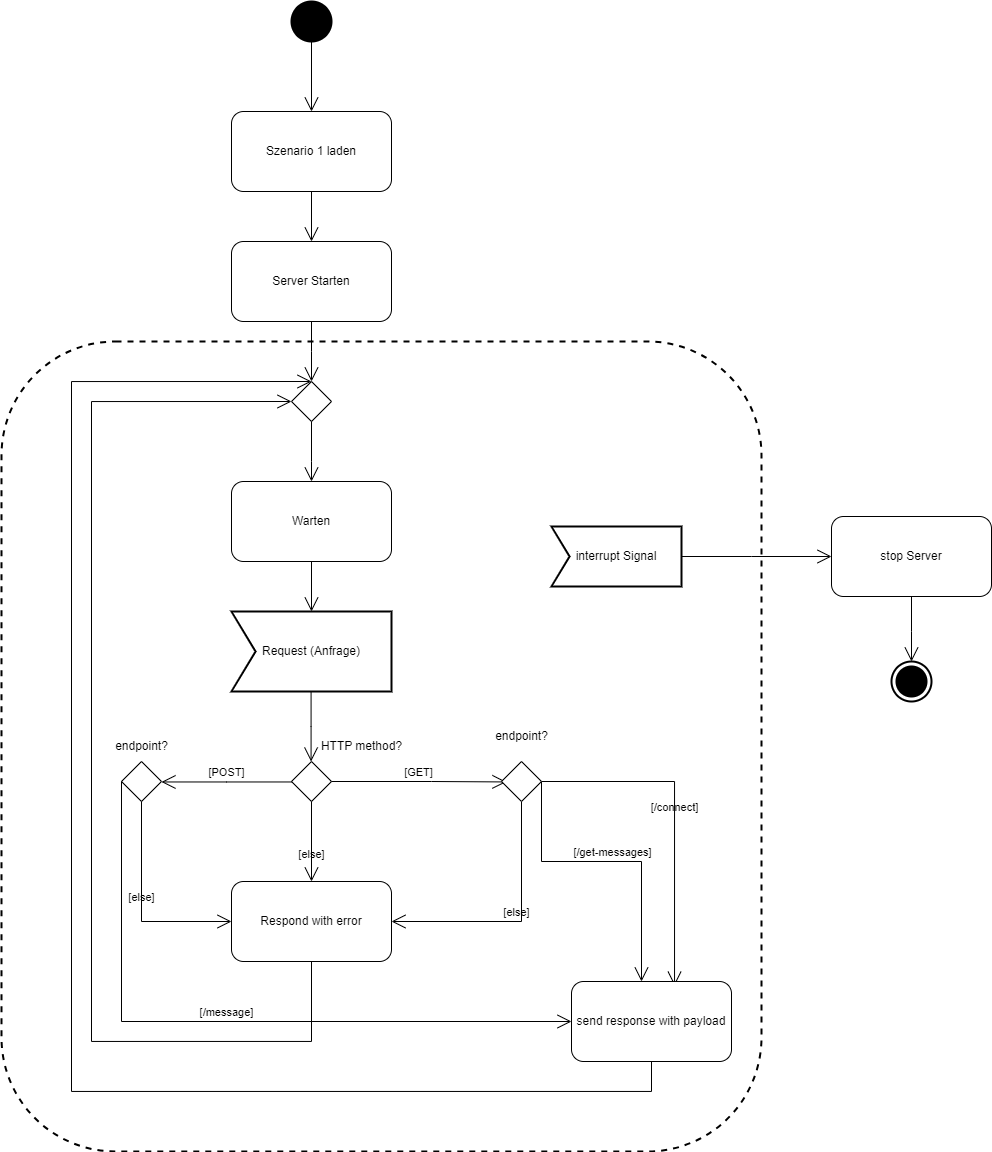
\includegraphics[scale=0.3]{images/serverStart.png}
    \caption{Ablaufdiagramm des Servers}
    \label{fig:protokoll}
\end{figure}


In Abbildung \ref{fig:protokoll} ist der Ablauf aller möglichen Szenarien dargestellt, wie eine solche Datenübertragung
zustande kommen kann. Im Folgenden werden die einzelnen Schritte und ihre Funktionen beschrieben:

\begin{itemize}
    \item \textbf{Start des Servers:} Auf der Hololens befindet sich ein Game-Objekt namens \textit{httpListener} mit einem
    Skript namens \textit{RequestManager.cs}. Beim Laden des ersten Szenarios wird ein HTTP-Listener in einem eigenen Thread
    gestartet. Erst wenn dieser läuft, kann auf Anfragen der Webseite reagiert werden.
    \item \textbf{Verbindungsaufbau:} Bevor ein Nachrichtenpaket gesendet werden kann, muss die IP-Adresse der Hololens
    registriert werden. Um zu testen, ob die richtige IP-Adresse eingegeben wurde oder der Server läuft, wird ein
    \texttt{http get request} an den Endpoint \textit{connect} gesendet.
    \item \textbf{Empfangen von Nachrichten:} Auf der Hololens wird eine Liste aktueller Nachrichten geführt. Die Webseite
    ruft alle fünf Sekunden mit einem \textit{http get request} an den Endpoint \textit{get-messages} diese Liste von Nachrichten ab.
    \item \textbf{Versenden von Nachrichten:} Um eine Nachricht von einem Laptop auf den anderen zu senden, muss ein
    \item \textit{http post request} an den Endpoint \textit{message} mit dem Benutzernamen und der Nachricht als Payload gesendet werden.
\end{itemize}

Das Senden von Requests mag kompliziert erscheinen, aber wie im Abschnitt \ref{sec:Frontend} zu sehen ist, wird dies
alles mithilfe einer benutzerfreundlichen UI erreicht.

Es ist festzuhalten, dass die beiden Laptops niemals direkt miteinander kommunizieren, sondern alle Nachrichten über den
Server, die Hololens, laufen.

\subsubsection{Bearbeitung von Anfragen}
Die Bearbeitung von Anfragen erfolgt im Skript \textit{RequestManager.cs}. Der Listener wird in einem eigenen Thread
gestartet, da das Warten auf Nachrichten den Thread, auf dem der Listener läuft, blockiert. Nach dem Erhalt einer Anfrage
wird ein neues \textit{HttpListenerContext}-Objekt erstellt, und die Verarbeitung der Anfrage erfolgt in dem Thread, der
diesen Kontext bearbeitet. Wenn eine HTTP-Anfrage empfangen wird, ist der erste Schritt, zu überprüfen, um welche Art von
Anfrage es sich handelt. Ein POST und ein GET werden unterschiedlich verarbeitet. Bei Verwendung einer anderen HTTP-Methode
wird ein \textit{Method Not Allowed} Fehler zurückgesendet. Bei der Wahl des Endpunkts passiert dasselbe; jede nicht
unterstützte Anfrage auf einen Endpunkt wird mit einem \textit{Not Found} Fehler beantwortet.

Es werden in unserem Fall nur drei Endpunkte unterstützt:

\begin{itemize}
    \item \textbf{Testen der Verbindung auf /connect}
    \item \textbf{Empfangen von Nachrichten auf /get-messages}
    \item \textbf{Senden einer Nachricht auf /message}
\end{itemize}

Um erfolgreich eine Anfrage an den Server zu senden, muss sie an die folgende Adresse
gehen: \texttt{http://{IP-Adresse der Hololens}:{Port}/{Endpoint}}. Die IP-Adresse der Hololens wird manuell auf der
Webseite eingegeben. Der Listener läuft standardmäßig auf dem Port 9090.

Die erlaubten Endpunkte sind wie oben aufgeführt fallbasiert gelistet.

\subsection{Object Tracking} \marginpar{\small\(\rightarrow\) SCHODITSCH}
Durch verwendung von bereitgestellten Technologien der HoloLens2
werden die zwei PCs und das Kabel getracked.
%Hier dann noch code zum Object Tracking einfügen

\subsection{Kurvenberechnung}
Durch Berechnung der Kurve wird das Kabel als Kurve gespeichert
und dadurch wird es ermöglicht, dass das 3D-Ping-Paket über diese
Kurve von einem PC zum anderen läuft.
%Hier dann noch code zur Kurvenberechnung einfügen

\section{Knapsack Problem Szenario} \marginpar{\small\(\rightarrow\) SKREPEK}
Im zweiten Anwendungsszenario dieser Applikation liegt der Fokus auf dem bekannten Problem des Knapsack-Problems. Ziel
dieses Szenarios ist es, dieses Informatikproblem mithilfe von Augmented Reality (AR) visuell und spielerisch darzustellen.
Das Knapsack-Problem ist ein klassisches Problem der Informatik, das nicht nur an der Höheren Technischen Lehranstalt (HTL)
vermittelt wird, sondern auch von Schülern eigenständig programmiert werden soll. Dieser Ansatz dient dazu, den Anwendern
einen Einblick in die Informatik zu geben und möglicherweise Interessen für den Bereich zu wecken.

Das Unity-Anwendungsszenario für die HoloLens 2 bietet insgesamt eine interaktive und visuelle Erfahrung, bei der der
Benutzer nicht nur das Knapsack-Problem verstehen, sondern auch praktisch anwenden kann. Die Integration von AR ermöglicht
es dem Benutzer, das Problem in einer realen Umgebung zu erleben und die Optimierungsmöglichkeiten direkt zu visualisieren
und zu manipulieren. Diese immersive Herangehensweise kann dazu beitragen, das Verständnis des Knapsack-Problems zu vertiefen
und das Interesse an der Informatik zu fördern.

In diesem Abschnitt werden alle \textit{GameObjects}, \textit{Komponenten}, \textit{Scripts} und \textit{Klassen} genauer
erklärt, die in der Unity-Szene des Knapsack-Problems verwendet werden, um dieses zu realisieren.

\subsection{Knapsack-Problem Szenrio Hirarchie} \marginpar{\small\(\rightarrow\) SKREPEK}
Für einen sicheren und funktionalen Ablauf ist der Aufbau beziehungsweise die Hirarchie der Unity Szene von großer Bedeutung.
In diesem Abschnitt wird anhand der Abbildung \ref{fig:level2_hierarchy} verdeutlich wie die Unity Szene für die Implementierung
des zweiten Anwendungsszenarios für das Knapsack-Problem aufgebaut ist und es wird zusätzlich kurz darauf eingegangen
für was welches Objekt steht und welche Aufgabe dieses trägt.
\\
\begin{figure}[H]
    \centering
    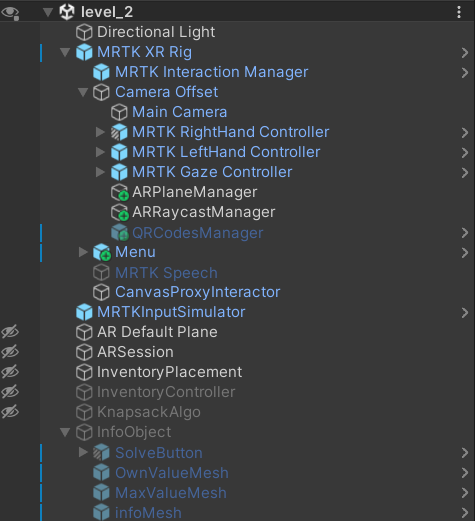
\includegraphics[scale=0.8]{images/Level2Hirarchy}
    \caption{Knapsack-Problem Szenario Hirarchie im Unity Editor.}
    \label{fig:level2_hierarchy}
\end{figure}
In dieser Abbildung ist die Hirarchie un der Inhalts des Knapsack-Problem Szenarios zu sehen. Anhand desen ist zu erkennen,
dass diese Unity Szene aus vielen wichtigen Komponenten besteht, die alle zusammenspielen, m das gewünschte Ergebnis
zu erzielen. Darunter sind folgende Objekte:
\begin{itemize}
    \item \textbf{level-2:} Ist die Unity Szene selbst, in der alle Game-Objekte enthalten sind.
    \item \textbf{MRTK XR Rig:} Grundbaustein für das Entwickeln einer XR-Applikation. Enthält wichtig Komponenten
    wie Controller für das tracken der Hände, für den User Gaze, etc.
    \item \textbf{UserInfo:} Text Objekt, dass in der \textit{main camera } liegt, damit dieses ständig im Sichtfeld des
    Benutzers liegt.
    \item \textbf{Managers:} Die drei Manager \textit{ARPlaneManager}, \textit{ARRaycastManager} und \textit{QRCodesManager}
    sind wichtiger Bestandteil um ARPlanes zu scannen, Raycasting durchzuführen und QRCodes zu erkennen.
    \item \textbf{HandMenu:} Knopf um in das Hauptmenu-Szenario zurück zu gelangen.
    \item \textbf{AR Default Plane:} Ist das Grund-Objekt für das markieren von erkannten ARPlanes.
    \item \textbf{ARSession:} Ist die Hauptkomponente, die die AR-Funktionalitäten steuert und koordiniert.
    \item \textbf{InventoryPlacementController:} Game Objekt, welches das platzieren des Inventar-Objekts handhabt.
    \item \textbf{InventoryController:} Game Objekt, welches das erkennen von neuen Objekten innerhalb des Inventar-Objekts handhabt.
    \item \textbf{KnapsackSolver:} Game Objekt, welches den Knapsack Algorithmus implementiert und das eigene Inventar berechnet.
    \item \textbf{bestSolutionPrefab:} Prefab, welches die perfekte Lösung wiederspiegelt.
    \item \textbf{InfoObject:} Dient der visualisierung von berechneten Werten und Fehlermeldungen.
\end{itemize}

In der Abbildung ist ausßredem zu sehen, dass ein Paar Game Objekte ausgegraut und nicht ausgegraut sind und, dass neben ein paar Game Objekten ein durchgestrichenes Auge zu sehen ist.
Wenn ein Game Objekt im Unity Editor ausgegraut ist bedeutet das, dass dieses GameObjekt und somit alle angehängiten Scripts von diesem Game Objekt deaktiviert sind.
Das bedeutet, dass dieses Game Objekt samt allen Scripts zu Szenenbeginn nicht aufgerufen und somit auch nicht ausgeführt werden. Nicht ausgegraute Game Objekte widerum sind
daher genau das Gegenteil. Das beudetet, dass das Game Objekt selbst samt allen angehängiten Scripts alle aktiviert sind und somit zu Szenenbeginn aufgerufen und ausgeführt werden.

Wenn neben einem Game Objekt das durchgestrichene Auge zu sehen ist bedeutet das nur, dass dieses Game Objekt im Unity Editor nicht zu sehen ist. Andererseits, wenn kein Zeichen
neben dem Game Objekt zu sehen ist, ist dieses Objekt im Unity Editor sichtbar. Dies dient dazu, dass falls in der Unity Szene viele Game Objekte vorhanden sind, dass man
diejenige ausblendet die nicht im Editor sichtbar sein müssen wie zum Beispiel Tesh Meshes oder Lables.

\subsection{Nutzung von QR-Codes} \marginpar{\small\(\rightarrow\) HAYLAZ}
Im vorherigen Abschnitt wurde bereits erwähnt, dass QR-Codes in diesem Level verwendet werden, um verschiedene Elemente
zu repräsentieren. Diese QR-Codes spielen eine entscheidende Rolle, indem sie dazu dienen, vielfältige Informationen zu
den einzelnen Objekten zu speichern und sie anschließend in einer virtuellen Umgebung abzubilden. Im folgenden Abschnitt
möchten wir näher darauf eingehen, wie genau diese QR-Codes generiert werden und welchen Zweck sie innerhalb der
Augmented Reality (AR)-Applikation erfüllen. Dabei wird insbesondere betrachtet, wie die Generierung der Codes erfolgt
und auf welche Weise sie innerhalb der Anwendung zur Interaktion mit den realen Objekten verwendet werden.

\subsubsection{Struktur und Inhalt eines QR-Codes}
Die Informationen, die in einem QR-Code gespeichert werden können, sind begrenzt. In unserem Anwendungsfall wird lediglich
eine einzelne Zahl im Bereich von 1 bis 11 abgespeichert. Diese Zahlen repräsentieren die 11 verschiedenen Modelle, die
wir unterscheiden möchten. Da nur eine Zahl gespeichert wird, genügt ein QR-Code der Größe 21x21 Module (Version 1). Die
geringe Anzahl von Modulen ermöglicht eine schnellere Erkennung, auch über größere Distanzen.

TODO: Testen und Grafik erstellen um zu zeigen das es eine Rolle spielt welche version wir verwenden + wie groß die sind

Die zugehörigen Zahlen erhalten in der Software, genauer gesagt in der Klasse \textit{QRItem.cs}, einen Kontext. Der folgende Codeausschnitt zeigt dies:

\begin{lstlisting}[style=csharp, caption={}, label=code:update]
public class QRItem
{
    public struct QRData
    {
        public int id;
        public string name;
        public Vector3 position;
        public int weight;
        public int value;
    }

    public QRData qrData;

    public Dictionary<int, QRData> items = new Dictionary<int, QRData>()
    {
        {1, new QRData { id = 1, name = "Laptop", weight = 70, value = 100 }},
        {2, new QRData { id = 2, name = "Router", weight = 25, value = 50 }},
        {3, new QRData { id = 3, name = "Maus", weight = 20, value = 30 }},
        // ...
        {11, new QRData { id = 11, name = "Handy", weight = 30, value = 100 }}
    };

    public QRItem(int id)
    {
        items.TryGetValue(id, out qrData);
    }
}
\end{lstlisting}

In dieser Klasse wird ein Dictionary verwendet, das den Zahlen die folgenden Informationen zuordnet:

\begin{itemize}
    \item \textbf{Item Id:} Die numerische Kennung im QR-Code.
    \item \textbf{Item Name:} Die Bezeichnung des Items, das dieser QR-Code repräsentiert.
    \item \textbf{Item Position:} Die Position des Items in der virtuellen Umgebung.
    \item \textbf{Item Weight:} Das Gewicht des Items.
    \item \textbf{Item Value:} Der Wert des Items.
\end{itemize}

Diese Informationen spielen eine wesentliche Rolle in der weiteren Berechnung des Knapsack-Algorithmus.

\subsubsection{QR-Code-Tracking}
Das Tracking der QR-Codes erfolgt mithilfe des \textit{QRCodeManager.cs} Skripts. Dieses Klasse ist ein Singleton, das
die Erkennung und Verfolgung der QR-Codes steuert.

Nach der Erkennung eines QR-Codes erfolgen eine Reihe von Schritten, um diese Informationen zu speichern, verarbeiten
und zuletzt darzustellen.
Hier eine kurze Übersicht:

\begin{figure}[H]
\centering
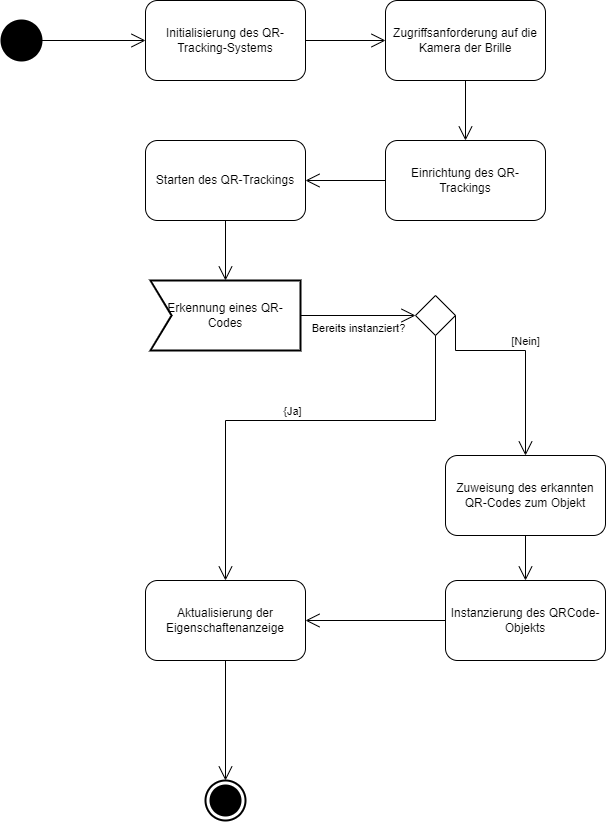
\includegraphics[scale=0.5, angle=0]{images/QRAblauf}
\caption{Ablaufdiagramm des QR-Code-Trackings.}
\label{fig:qrtracking}
\end{figure}

\begin{itemize}

\item \textbf{Initialisierung des QR-Tracking-Systems:}
Zur Aktivierung des QR-Tracking-Systems werden die erforderlichen Ressourcen und Komponenten gestartet, um die Erkennung
von QR-Codes zu ermöglichen. Dabei werden Tracking-Algorithmen gestartet, die für die Lokalisierung und Identifizierung
von QR-Codes in der Umgebung benötigt werden. Diese Initialisierung erfolgt zu Beginn der Anwendungsaktivität.

\item \textbf{Zugriffsanforderung auf die Kamera der Brille:}
TODO: Hier ein Bild von "Camera acess needed" einfügen
Für das QR-Tracking wird der Zugriff auf die Kamera der Augmented-Reality-Brille benötigt. Eine Zugriffsanfrage wird
gestellt, um die notwendigen Berechtigungen zu erhalten. Dieser Schritt ist entscheidend, um visuelle Daten von der Kamera
zu erhalten und QR-Codes in der physischen Umgebung zu erkennen.

\item \textbf{Einrichtung des QR-Trackings:}
Die Einrichtung des QR-Trackings umfasst die Konfiguration von Parametern und Einstellungen, die für die korrekte
Funktion des Tracking-Systems erforderlich sind.Dazu gehören Kalibrierungsschritte, die Anpassung an die Umgebung und die
Festlegung von Erkennungsbereichen. Eine ordnungsgemäße Einrichtung gewährleistet eine zuverlässige und präzise Erkennung von QR-Codes.

\item \textbf{Starten des QR-Trackings:}
Das System sucht aktiv nach QR-Codes in der Umgebung, um sie zu erkennen. Die Kamera erfasst kontinuierlich visuelle
Daten, welche von den Tracking-Algorithmen analysiert werden, um QR-Codes zu identifizieren. Das Starten des Trackings
markiert den Beginn des fortlaufenden Erkennungsprozesses.

\item \textbf{Erkennung eines QR-Codes (Event):}
Sobald die Kamera einen QR-Code erfasst, wird dieser erkannt. Das Ereignis signalisiert, dass ein QR-Code erkannt wurde
und gibt Informationen über den erkannten QR-Code, wie seine Daten und Position, weiter.

\item \textbf{Zuweisung des erkannten QR-Codes zum Objekt:}
Nach der Erkennung wird überprüft, ob der erkannte QR-Code bereits in der Anwendung registriert ist. Falls dies der Fall
ist, wird der erkannte QR-Code einem entsprechenden Objekt in der virtuellen Umgebung zugeordnet.

\item \textbf{Instanzierung des QRCode-Objekts:}
Nach dem Scannen eines QR-Codes wird ein QR-Code-Prefab erzeugt und in der Szene platziert.

Dieses Objekt dient als Repräsentation des gescannten QR-Codes und wird als QR-Objekt bezeichnet. Es enthält visuelle
Darstellungen, Interaktionsmöglichkeiten und weitere relevante Informationen über den zugehörigen QR-Code. Die Instanziierung
ermöglicht eine nahtlose Integration des gescannten QR-Codes in die virtuelle Umgebung. Weitere Informationen zur Visualisierung
von QR-Codes finden Sie in Abschnitt \ref{sec:qr_visualization}.

\item \textbf{Aktualisierung der Eigenschaftenanzeige:}
Die Aktualisierung der Eigenschaftsanzeige dient dazu, visuelle und informative Darstellungen des erkannten QR-Codes zu
aktualisieren. Hierbei werden die Position, Größe, visuelle Darstellung und zugehörige Informationen des QR-Codes aktualisiert.
Durch die Aktualisierung wird sichergestellt, dass die Benutzer stets die neuesten Informationen über das durch den QR-Code
repräsentierte Objekt erhalten.

\end{itemize}

\subsubsection{Interaktion mit QR-Codes}
\begin{figure}[H]
\centering
\includegraphics[scale=0.04, angle=0]{images/bauklotz}
\caption{Bauklötze mit QR-Codes}
\label{fig:bauklotz}
\end{figure}
TODO: neues besseres Bild einfügen

Durch die Verwendung der HoloLens können wir dem Benutzer eine visuelle Darstellung einer virtuellen Welt bieten. Um eine
Verbindung zwischen der realen und der virtuellen Welt herzustellen, nutzen wir QR-Codes.  Diese dienen als Repräsentationen
der realen Objekte, die wir in der virtuellen Welt darstellen möchten.

Wie in \ref{fig:bauklotz} zu sehen ist, sind die Bauklötze mit QR-Codes versehen. Diese Bauklötze repräsentieren die Gegenstände,
die der Benutzer in sein Inventar aufnehmen kann. Wenn der Benutzer einen Bauklotz aufhebt und ihn der HoloLens nähert, wird
der QR-Code gescannt. Dadurch werden Informationen wie das zugehörige 3D-Modell, der Wert, das Gewicht und der Name des
Gegenstands angezeigt. Auf diese Weise können wir eine nahtlose Verbindung zwischen der realen und der virtuellen Welt
herstellen und dem Benutzer eine interaktive Erfahrung bieten.

Dem Benutzer wird die Möglichkeit geboten, die Bauklötze physisch zu berühren, aufzuheben und zu fühlen. Diese sensorische
Erfahrung trägt dazu bei, die Immersion des Benutzers zu verbessern und ihm ein besseres Verständnis der virtuellen Welt
zu ermöglichen.

\subsubsection{Bestimmen der Position QR-Codes}
TODO: Auch die events add remove und update erklären vom qrWatcher

\subsubsection{Visualisierung von QR-Codes}
TODO: Bild von einem QR Prefab einfügen
Nachdem die genaue Platzierung der QR-Codes bestimmt wurde, steht die Aufgabe an, ihre Visualisierung in der virtuellen Welt umzusetzen.

Hierfür wird die Funktionalität von Unity Prefabs genutzt. Diese ermöglichen die Erstellung visueller Repräsentationen
der QR-Codes und ihre nahtlose Integration in die virtuelle Umgebung. Weitere Informationen zu Prefabs und ihrer Funktionsweise
finden Sie im Abschnitt \ref{Unity Prefabs}.

Innerhalb jedes Prefabs sind alle relevanten Informationen enthalten, die für die korrekte Darstellung des QR-Codes
erforderlich sind. Dazu gehören nicht nur das 3D-Modell des QR-Codes, sondern auch zugehörige Daten wie Name, Wert und
Gewicht. Diese Daten sind entscheidend für die Interaktionen innerhalb der virtuellen Umgebung.

Um die Funktionalität des QR-Codes in der virtuellen Welt zu gewährleisten, wird dem Prefab das Skript \textit{QRCodes.cs} zugewiesen.
Dieses Skript steuert die visuelle Darstellung des QR-Codes sowie sämtliche Interaktionen, die damit verbunden sind. Durch
die Zuweisung dieses Skripts wird sichergestellt, dass die QR-Codes nicht nur korrekt angezeigt, sondern auch innerhalb
der virtuellen Umgebung interaktiv sind.

TODO: Bild von einem gescannten QRCode einfügen

\subsubsection{Zugriff auf QR-Codes bereitstellen}
Wie bereits im Abschnitt \ref{sec:KnapSackProblem} erwähnt, benötigen andere Teile der Anwendung Zugriff auf
die aktuell erkannten QR-Codes in der Szene, um entsprechend darauf reagieren zu können. Die Bereitstellung dieser Option war eine Herausforderung.
Um keine Performance-Einbußen auf der Hololens zu verursachen, läuft der Prozess des QR-Code-Trackings auf
mehreren Threads. Die aktuell erkannten QR-Codes werden in einem SortedDictionary gespeichert, welches von anderen Teilen
der Anwendung abgefragt werden kann. Da auf dieses Objekt von mehreren Threads zugegriffen wird, muss es mit einem
\textit{lock} geschützt werden, um inkonsistenzen zu vermeiden. Hierbei handelt es sich um eine Sperre, die verhindert,
dass mehrere Threads gleichzeitig auf das gleiche Objekt zugreifen. Auf diese Weise wird sichergestellt, dass die Daten
nicht inkonsistent werden und dass die Anwendung stabil und zuverlässig bleibt. Jedoch da wir Threads zugriff verweigern
müssen, um die Daten zu schützen, kann es zu einer Verzögerung kommen, bis die Daten verfügbar sind. Jedoch ist dieser
Nachteil in unserem Anwendungsfall nicht von großer Bedeutung da wir selten zur gleichen Zeit auf die Daten zugreifen und
dadurch die Verzögerung nicht bemerkbar ist.

\subsection{Platzieren des Inventars}\marginpar{\small\(\rightarrow\) SKREPEK}
Um eine präzise Interaktion zwischen der realen und augmentierten Realität zu gewährleisten, ist der Zugriff auf die Kamera
erforderlich, um die physische Umgebung präzise zu erfassen. Durch die Analyse der erfassten Umweltdaten können relevante
Ebenen identifiziert werden, die entscheidend sind, um eine akkurate Platzierung des Inventar-Objekts zu gewährleisten.

In diesem Abschnitt wird auf das \textit{inventoryPlacementController} Unity Game Objekt mit der zugehörigen Komponenten
\textit{InventoryPlacementController.cs} Skript behandelt. Dieses Skript implementiert die \textbf{InventoryPlacementController}
Klasse welche sämtliche Funktion zu Berechnung der Position und Platzierung des Inventar Objekts umfasst.

\subsubsection{Das inventoryPlacementController Game Objekt}
Das inventoryPlacementController Game Objekt in folgender Abbildung \ref{fig:inventoryPlacementController_Editor}
ist der Grundbaustein für das Anwendungsszenario des Knapsack-Problems. Es ist dafür zuständig, anhand des  Blicks des
Benutzers das Invenar Objekt dementsprechend richtig zu platzieren und zu visualisieren. Das Game Objekt hat eine angehängte
Komponente \textit{inventoryPlacementController.cs} welche das Skript für die Implementierung dieser Logik wiederspiegelt
und die \textbf{InventoryPlacementController} Klasse implementiert.

\begin{figure}[H]
    \centering
    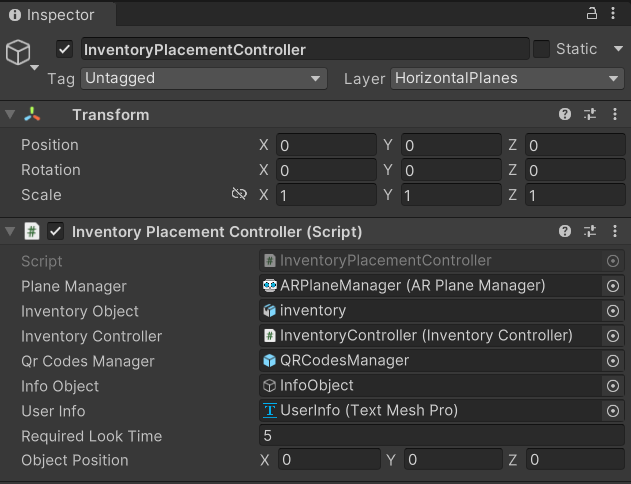
\includegraphics[scale=0.8]{images/invPlace_Editor}
    \caption{inventoryPlacementController Objekt im Editor}
    \label{fig:inventoryPlacementController_Editor}
\end{figure}

Diese Abbildung veranschaulicht das Game Objekt im Unity Inspektor. Wie hier veranschaulicht wird, bietet diese Komponente
einige Dinge, die direkt in Unity angegeben und übergeben werden können. Darunter wichtig sind vorallem die Variablen der
Klasse selbst, die Objekte aus dem Unity Editor benötigen, um dementsprechend funktionieren zu können. Diese Variablen umfassen:
\begin{itemize}
    \item \textbf{Plane Manager:} Hierbei handelt es sich um eine Zuweisung zum Game Objekt des \textit{ARPlanesManagers}
    aus der Szene Level 2.
    \item \textbf{Inventory Object:} Diese Referenz ist mit dem 3D-Modell des Inventars aus dem Prefab-Ordner verknüpft.
    \item \textbf{Inventory Controller:} Diese Variable ist mit dem Skript des \textit{InventoryControllers} verbunden.
    \item \textbf{QR Codes Manager:} Hierbei handelt es sich um einen Verweis auf das Game Objekt des \textit{QRCodeManagers}
    aus der Szene Level 2.
    \item \textbf{Info Object:} Diese Referenz ist mit dem Game Objekt \textit{infoObject} aus der Szene Level 2 verbunden.
    \item \textbf{User Info:} Referenz auf das TextMesh in der \textit{Main Camera}, dass zur Anzeige von Anweisungen und
    Tipps dient.
    \item \textbf{Required Look Time:} Diese Variable gibt die vorgeschriebene Zeitdauer an, für die der Benutzer auf ein
    Plane blicken muss, damit das Inventar platziert wird.
\end{itemize}

\subsubsection{User Gaze in AR-Anwendungen}
Die Verwendung des Benutzerblicks bildet die Grundlage für das Anwendungsszenario des Knapsack-Problems. Gaze bezieht sich
auf die Richtung und Position, in die eine Person ihren Blick richtet, und ermöglicht die Analyse der Aufmerksamkeit des
Benutzers in der realen Welt. Diese Information wird genutzt, um festzustellen, wohin der Benutzer schaut, und damit die
Platzierung des Inventar Objekts in der virtuellen Umgebung zu bestimmen. Darüber hinaus eröffnet die Verwendung des Gazes
eine Vielzahl weiterer Möglichkeiten.

\begin{enumerate}
    \item \textbf{Interaktionen basierend auf dem Blick}: Durch die Verfolgung des Benutzergazes können Interaktionen in
    der AR-Umgebung ausgelöst werden. Beispielsweise kann der Benutzer durch simples Anschauen eines virtuellen Objekts
    darauf klicken, um weitere Informationen anzuzeigen oder eine Aktion auszulösen. Diese Art der Interaktion ermöglicht
    eine intuitive Bedienung ohne physische Eingabegeräte.

    \item \textbf{Blickgesteuerte Navigation}: Die HoloLens 2 ermöglicht auch eine blickgesteuerte Navigation in der
    AR-Umgebung. Indem der Benutzer bestimmte Punkte oder Objekte anschaut, kann er beispielsweise in der Umgebung navigieren
    oder Menüs öffnen, ohne physische Gesten ausführen zu müssen.

    \item \textbf{Verbesserte Immersion}: Die Integration des Gaze in AR-Anwendungen mit der HoloLens 2 trägt zur Immersion
    des Benutzers bei, indem sie die Interaktion mit der virtuellen Umgebung natürlicher und nahtloser gestaltet. Durch die
    genaue Erfassung des Benutzergazes und die Echtzeitreaktion auf virtuelle Objekte entsteht ein Gefühl von Präsenz und
    Realismus.
\end{enumerate}

\subsubsection{InventoryPlacementController Klasse}
Die \textbf{InventoryPlacementController} Klasse ist ein zentraler Bestandteil der AR-Anwendung, die für das Knapsack-Problem
Szenario entwickelt wurde. Diese Klasse ist verantwortlich für die Platzierung des Inventar Objekts basierend auf dem
Benutzergaze in der virtuellen Umgebung. Sie ermöglicht die Interaktion mit AR-Planes und steuert den Prozess der Platzierung
von dem Inventar Objekt auf einem ausgewählten \textit{ARPlane}. Die Klasse enthält Funktionen zur Erfassung des Benutzergazes, zur
Auswahl geeigneter Ebenen für die Platzierung und zur Ausführung der Platzierungslogik. Durch die Integration dieser
Klasse wird eine nahtlose und intuitive Benutzererfahrung für die AR-Anwendung gewährleistet. Die Klasse sieht wie folgt aus:
\begin{lstlisting}[caption={InventoryPlacementController Klasse}, label=code:isPOP]
public class InventoryPlacementController : MonoBehaviour
{
    public ARPlaneManager planeManager;
    public GameObject inventoryObject;
    public InventoryController inventoryController;
    public GameObject qrCodesManager;
    public GameObject infoObject;
    public TextMeshPro userInfo;
    public float requiredLookTime = 5.0f;
    public Vector3 objectPosition;

    private ARPlane selectedDeskPlane;
    private float lookStartTime = -1f;
    private bool objectPlaced = false;
    private float heightOffset = 0.001f;

    private bool canStartScript = false;

    private IEnumerator DelayedStart(){...}

    void Start(){...}

    void Update(){...}

    private bool IsPointerOverPlane(){...}

    private ARPlane GetCurrentPlaneUnderGaze(){...}

    private void PlaceObjectOnDesk(ARPlane deskPlane){...}
}
\end{lstlisting}\\
\\
Im Folgenden werden die drei wichtigen Funktionen \textbf{Update()}, \textbf{IsPointerOverPlane()} und \textbf{PlaceObjectOnDesk()}
näher erläutert, um ein tieferes Verständnis für die zugrunde liegende Logik zu vermitteln.

\subsubsection{Verwendung des Usergazes}
In dieser Klasse wird der Blick des Benutzers in zwei separaten Funktionen verwendet, um das \textit{ARPlane} zu identifizieren,
auf das der Benutzer gerade schaut. Beide Funktionen basieren auf derselben grundlegenden Logik, unterscheiden sich jedoch
darin, dass die Funktion \textbf{IsPointerOverPlane()} einen booleschen Wert zurückgibt, der angibt, ob sich der
Benutzergaze über einem \textit{ARPlane} befindet, während die Funktion \textbf{GetCurrentPlaneUnderGaze()} das tatsächliche
identifizierte \textit{ARPlane} zurückgibt. Um die zugrunde liegende Logik des Benutzergazes zu verdeutlichen, wird anschließend
die Funktionsweise der \textbf{IsPointerOverPlane()} Funktion erläutert.
\begin{lstlisting}[caption={Funktion um Usergaze zu verwenden}, label=code:isPOP]
private bool IsPointerOverPlane()
{
    Ray ray = Camera.main.ScreenPointToRay(Input.mousePosition);
    RaycastHit hit;
    if (Physics.Raycast(ray, out hit))
    {
        ARPlane plane = hit.collider.GetComponent<ARPlane>();
        return (plane != null);
    }
    return false;
}
\end{lstlisting}\\
Die Funktion verwendet eine Raycast-Abfrage, um festzustellen, ob sich der Benutzergaze über einem \textit{ARPlane} befindet.

In dieser Funktion wird zuerst ein Ray erstellt, der vom Hauptkamerapunkt ausgeht und durch den aktuellen Mauszeiger verläuft
(der die Position des Benutzergazes repräsentiert). Dieser Ray wird verwendet, um festzustellen, ob er mit einem Objekt
in der Szene kollidiert.

Wenn der Ray auf ein Objekt trifft (dargestellt durch die Variable \textit{hit}), wird überprüft, ob es sich bei diesem
Objekt um ein \textit{ARPlane} handelt. Dies wird durch den Aufruf von \textit{hit.collider.GetComponent<ARPlane>()}
überprüft. Wenn das Objekt ein \textit{ARPlane} ist, wird die Funktion \textit{GetComponent<ARPlane>()} nicht null
zurückgeben, was bedeutet, dass sich der Benutzergaze über einem \textit{ARPlane} befindet, und die Funktion gibt true
zurück.

Wenn der Ray auf kein \textit{ARPlane} trifft oder überhaupt kein Objekt getroffen wird, wird false zurückgegeben, was
bedeutet, dass sich der Benutzergaze nicht über einem \textit{ARPlane} befindet.

\subsubsection{Frame Aktualisierung}
Während der Ausführung dieses Skripts kann der Benutzer seinen Blick auf ein anderes \textit{ARPlane} lenken, weshalb es
wichtig ist, kontinuierlich zu überprüfen, ob das Inventarobjekt bereits platziert wurde. Diese Überprüfung wird durch
die \textbf{Update()} Funktion durchgeführt, die in jedem Frame aufgerufen wird, was bedeutet, dass sie mit einer Frequenz
von 60 Mal pro Sekunde ausgeführt wird. Die \textbf{Update()} Funktion ist von zentraler Bedeutung für dieses Skript, da
sie die Platzierung des Inventarobjekts anhand des Benutzergazes überwacht und aktualisiert. Um die Funktionsweise dieser
Funktion genauer zu erläutern, wird im Folgenden näher darauf eingegangen.
\begin{lstlisting}[caption={Funktion um Usergaze zu verwenden}, label=code:isPOP]
void Update()
{
    if (!objectPlaced && canStartScript)
    {
        if (IsPointerOverPlane())
        {
            ARPlane currentPlane = GetCurrentPlaneUnderGaze();

            if (currentPlane != null)
            {
                if (selectedDeskPlane == null || selectedDeskPlane != currentPlane)
                {
                    selectedDeskPlane = currentPlane;
                    lookStartTime = Time.time;
                }
                float timeLookedAtPlane = Time.time - lookStartTime;
                userInfo.text = ((int)requiredLookTime - (int)timeLookedAtPlane).ToString();
                if (timeLookedAtPlane >= requiredLookTime)
                {
                    PlaceObjectOnDesk(selectedDeskPlane);
                    objectPlaced = true;
                    userInfo.text = "";
                }
            }
            else
            {
                selectedDeskPlane = null;
                userInfo.text = "Schauen Sie auf einen Tisch";
            }
        }
        else
        {
            selectedDeskPlane = null;
            userInfo.text = "Schauen Sie auf einen Tisch";
        }
    }
}
\end{lstlisting}\\
Die Funktionsweise der \texttt{Update()} Funktion lässt sich in mehrere Schritte gliedern:

\begin{enumerate}
    \item \textbf{Überprüfung, ob das Inventar Objekt noch nicht platziert wurde und das Skript gestartet werden kann}:
    Zunächst wird in der \textbf{Update()} Funktion überprüft, ob das Inventar Objekt bereits platziert wurde (\textit{objectPlaced}),
    und ob das Skript gestartet werden kann (\textit{canStartScript}). Dies stellt sicher, dass die Platzierung nur dann
    durchgeführt wird, wenn beide Bedingungen erfüllt sind.

    \item \textbf{Bestimmung des Benutzergaze über einem ARPlane}: Anschließend wird geprüft, ob sich der Benutzergaze
    über einem ARPlane befindet. Dies wird durch den Aufruf der Funktion \textbf{IsPointerOverPlane()} erreicht, die
    feststellt, ob sich der Benutzergaze über einem ARPlane befindet.

    \item \textbf{Identifikation des aktuellen ARPlane}: Wenn bestätigt wird, dass sich der Benutzergaze über einem ARPlane
    befindet, wird der aktuelle ARPlane identifiziert. Dies erfolgt durch den Aufruf der Funktion \textit{GetCurrentPlaneUnderGaze()},
    die den ARPlane bestimmt, auf den der Benutzergaze gerichtet ist.

    \item \textbf{Aktualisierung des ausgewählten ARPlane und Startzeit des Blicks}: Nachdem der ARPlane identifiziert wurde,
    wird überprüft, ob es sich um einen anderen ARPlane handelt als den, auf den der Benutzergaze zuletzt gerichtet war.
    Falls ja, wird die Variable \textit{selectedDeskPlane} aktualisiert und die Startzeit des Blicks auf den neuen ARPlane gespeichert.

    \item \textbf{Messung der Blickdauer auf den aktuellen ARPlane}: Es wird die Dauer gemessen, für die der Benutzer auf
    den aktuellen ARPlane schaut. Dies erfolgt durch die Berechnung der Zeitdifferenz seit dem Start des Blicks auf den ARPlane.

    \item \textbf{Überprüfung, ob die erforderliche Blickdauer erreicht wurde}: Es wird überprüft, ob die gemessene Zeit
    die erforderliche Zeit überschreitet, die der Benutzer auf den ARPlane schauen muss, um das Inventarobjekt zu platzieren.

    \item \textbf{Platzierung des Inventarobjekts}: Wenn die erforderliche Blickdauer erreicht wurde, wird die Funktion
    \textbf{PlaceObjectOnDesk()} aufgerufen, um das Inventarobjekt auf dem ausgewählten ARPlane zu platzieren.

    \item \textbf{Aktualisierung des Platzierungsstatus und der Benutzeroberfläche}: Nach erfolgreicher Platzierung des
    Objekts wird die Variable \textit{objectPlaced} auf \textit{true} gesetzt, um anzuzeigen, dass das Objekt platziert
    wurde. Außerdem wird die Benutzeroberfläche entsprechend aktualisiert, um den Benutzer über den erfolgreichen Platzierungsvorgang
    zu informieren.

    \item \textbf{Benachrichtigung bei fehlendem ARPlane}: Wenn der Benutzergaze sich nicht über einem ARPlane befindet
    oder kein ARPlane erkannt wird, wird die Benutzeroberfläche entsprechend aktualisiert, um den Benutzer darüber zu
    informieren, dass er auf einen ARPlane schauen muss, um das Inventarobjekt erfolgreich zu platzieren.
\end{enumerate}

\subsubsection{Platzieren des Inventar Objekts}
Das Platzieren des Inventarobjekts markiert das Ende des \textit{InventoryPlacementController} Skripts. Die Funktion
\textbf{PlaceObjectOnDesk()} übernimmt die Aufgabe, das Inventarobjekt zu platzieren und weitere Gameobjekte sowie
Skripts zu aktivieren oder zu deaktivieren, um einen reibungslosen Fortlauf der Anwendung zu gewährleisten. Im folgenden
Code-Ausschnitt wird die Implementierung der \textbf{PlaceObjectOnDesk()} Funktion dargestellt:
\begin{lstlisting}[caption={Funktion zum Platzieren des Inventarobjekts}, label=code:isPOP]
private void PlaceObjectOnDesk(ARPlane deskPlane)
{
    qrCodesManager.SetActive(true);
    objectPosition = deskPlane.center + Vector3.up * heightOffset;
    Quaternion objectRotation = Quaternion.Euler(-90f, 0f, 0f);
    GameObject instantiatedObject = Instantiate(inventoryObject, objectPosition, objectRotation);
    instantiatedObject.transform.localScale = new Vector3(20f, 20f, 20f);
    Vector3 infoObjectPosition = objectPosition - Vector3.forward * 4.415f + Vector3.right * 0.4f;
    infoObject.transform.position = infoObjectPosition;
    infoObject.SetActive(true);
    inventoryController.SetInventoryObject(instantiatedObject);
    inventoryController.gameObject.SetActive(true);
    gameObject.SetActive(false);
}
\end{lstlisting}\\
Im Wesentlichen kann diese Funktion in mehrere einzelne Schritte unterteilt werden, die den Platzierungsvorgang des
Inventarobjekts steuern:

\begin{enumerate}
    \item \textbf{Aktivierung des QRCodesManagers:} Zunächst wird der QRCodesManager aktiviert, um sicherzustellen, dass
    QR-Codes nach Abschluss dieses Skripts gescannt werden können.

    \item \textbf{Berechnung der Position und Anpassung der Skalierung:} Als nächstes wird die Position des zu platzierenden
    Objekts anhand der Mitte des übergebenen \textit{ARPlane} berechnet. Die Rotation wird auf eine standardmäßige
    Ausrichtung eingestellt, und das Objekt wird instanziiert, um es für den Benutzer sichtbar zu machen. Abschließend
    wird die Skalierung des Objekts auf einen festgelegten Wert gesetzt, um die Größe des Inventarobjekts zu steuern.

    \item \textbf{Platzierung des Informationsobjekts:} Die Position des Informationsobjekts wird berechnet, damit es
    neben dem Inventar Objekt platziert wird. Anschließend wird das Informationsobjekt aktiviert, um es sichtbar zu machen
    und dem Benutzer zusätzliche Informationen zu liefern.

    \item \textbf{Übergabe des Inventar Objekts an den Inventory Controller:} Die Instanz des Inventarobjekts wird dem
    Inventory Controller übergeben, um sicherzustellen, dass dieser mit der richtigen Instanz des Objekts arbeitet und die
    Interaktion ordnungsgemäß durchgeführt werden kann.

    \item \textbf{Aktivierung des Inventory Controllers:} Nach Abschluss der Platzierungsvorgänge wird das Inventory
    Controller Skript aktiviert, um die Interaktion mit dem Inventar zu ermöglichen.

    \item \textbf{Deaktivierung des Inventory Placement Controllers:} Abschließend wird das InventoryPlacementController
    Gameobjekt selbst deaktiviert, da seine Aufgabe erfüllt ist und das Inventarobjekt erfolgreich platziert wurde.
\end{enumerate}

Diese Schritte führen den Platzierungsvorgang des Inventarobjekts durch und stellen sicher, dass die Anwendung ordnungsgemäß
funktioniert und dem Benutzer eine nahtlose und intuitive Benutzererfahrung bietet.

\subsubsection{Sicht des Benutzers nach Abschluss des Skripts}
Nach Abschluss des Skripts zur Platzierung des Inventarobjekts hat der Benutzer eine klare Sicht auf die virtuelle Umgebung.
Das platzierte Objekt wird nun auf der Oberfläche angezeigt, auf die der Benutzer seinen Blick gerichtet hat, wodurch
eine nahtlose Integration von virtuellen und physischen Elementen entsteht.

Die Platzierung des Inventar Objekts ermöglicht es dem Benutzer, eine immersive Erfahrung zu erleben, bei der virtuelle
und reale Elemente nahtlos miteinander verschmelzen. Diese Integration schafft eine reichhaltige und interaktive Augmented-Reality-Umgebung,
die es dem Benutzer ermöglicht, mit den virtuellen Objekten in seiner physischen Umgebung zu interagieren.

Ein visuelles Beispiel dieser Erfahrung ist in Abbildung \ref{fig:inventoryPlaced} dargestellt, die die Sicht des Benutzers
nach der Platzierung des Inventar Objekts veranschaulicht.

\begin{figure}[H]
    \centering
    \includegraphics[scale=0.8]{images/invPlaced}
    \caption{Sicht des Benutzers nach Platzierung des Inventars}
    \label{fig:inventoryPlaced}
\end{figure}

\subsection{Inventarverwaltung}\marginpar{\small\(\rightarrow\) SKREPEK}
Die effiziente Verwaltung des platzierten Inventar Objekts ist entscheidend für das Anwendungsszenario des Rucksack-Problems.
Die kontinuierliche Überwachung und Aktualisierung des Inventars in Echtzeit ermöglicht es, Änderungen wie das Hinzufügen
oder Entfernen von Gegenständen durch den Benutzer zu verfolgen. Dieser Abschnitt behandelt das Unity Game Objekt
\textit{InventoryController} und das zugehörige Skript \textit{InventoryController.cs}, welches die \textbf{InventoryController}
Klasse implementiert, um diese Aufgaben zu lösen.

\subsubsection{Das InventoryController Game Objekt}
Das InventoryController Game Objekt ist das zentrale Element für die Verwaltung des Inventars und ermöglicht eine nahtlose
Interaktion zwischen dem Inventar und platzierten bzw. entfernten Gegenständen. Es überwacht kontinuierlich das Inventar,
um Veränderungen zu erkennen und darauf zu reagieren. Ausgestattet mit der Komponente \textit{InventoryController.cs},
führt es logische Operationen aus und stellt die Funktionalitäten der Klasse \textbf{InventoryController} bereit.

\begin{figure}[H]
    \centering
    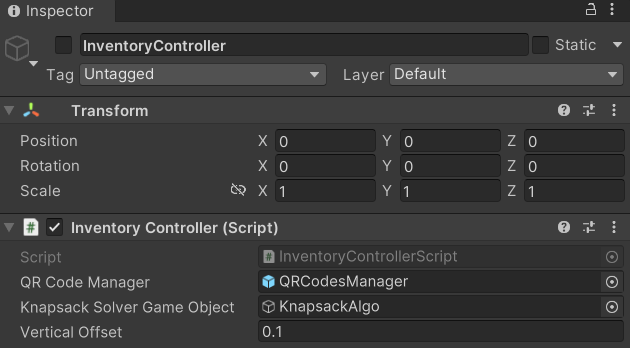
\includegraphics[scale=0.8]{images/invCon_Editor}
    \caption{InventoryController Objekt im Editor}
    \label{fig:InventoryController_Editor}
\end{figure}

Das InventoryController Game Objekt im Unity Inspektor bietet Einstellungen, die direkt in Unity angepasst werden können.
Wichtige Variablen, die auf Objekte aus dem Unity Editor verweisen müssen, sind:
\begin{itemize}
    \item \textbf{QRCodesManager:} Referenz auf das \textit{QRCodesManager}-Game-Objekt aus der Level 2 Szene.
    \item \textbf{Knapsack Solver Game Objekt:} Referenz auf das \textit{KnapsackAlgo}-Game-Objekt aus der Level 2 Szene.
    \item \textbf{User Info:} Referenz auf das TextMesh in der \textit{Main Camera}, das zur Anzeige von Anweisungen und Tipps dient.
    \item \textbf{Vertical Offset:} Float-Wert, um den die Begrenzungen (\textit{Bounds}) des Inventory-Objekts auf der X-Achse erweitert werden.
\end{itemize}

Diese Konfiguration ermöglicht eine effektive Kommunikation zwischen dem InventoryController und anderen Komponenten der
Applikation, um eine reibungslose Funktionalität des Inventars sicherzustellen.

\subsubsection{InventoryController Klassenvariablen}
\begin{lstlisting}[style=csharp, caption={Klassenvariablen der InventoryController Klasse}, label=code:controller_var]
public GameObject QRCodeManager;
public GameObject knapsackSolverGameObject;
public TextMeshPro userInfo;
public float verticalOffset = 0.1f;

private SortedDictionary<System.Guid, GameObject> activeQRObjects;

private GameObject inventoryObject;
private Bounds inventoryBounds;
private int numRows = 3;
private int numColumns = 3;
private int[,] idGrid;
private KnapsackSolver knapsackSolver;
private int cap;
private int currWeight = 0;
private HashSet<int> processedItems;
\end{lstlisting}\\
Die gezeigten Klassenvariablen im Codeabschnitt \ref{code:controller_var} sind Teil der \textit{InventoryController} Klasse.
Öffentliche (\textit{public}) Variablen repräsentieren Objekte und Werte, die im Unity Editor festgelegt und übergeben
werden oder von anderen Klassen für die Funktionalität benötigt werden. Dies ermöglicht einen direkten Zugriff auf diese
Objekte in der eigenen oder einer anderen Klasse. Die Float-Variable \textit{verticalOffset} spielt hier eine wichtige Rolle
für die Erweiterung der Begrenzungen (\textit{Bounds}) des Inventar-Modells und das TextMeshPro \textit{userInfo} für das
anzeigen von Anweisung und Tips für den Benutzer.

Die privaten (\textit{private}) Variablen dienen der lokalen Speicherung von Werten, die von keiner anderen Klasse benötigt
werden.

\subsubsection{Start des InventoryControllers}
Die \textbf{Start()} Funktion spielt eine Schlüsselrolle beim Initialisieren der erforderlichen Objekte und Skripte für den
erfolgreichen Start des \textit{InventoryControllers}. Diese Funktion wird zu Beginn des \textit{InventoryControllers}
aufgerufen und ist verantwortlich für die Deklaration und Einrichtung der notwendigen Komponenten. Entsprechender Code
dieser Funktion:
\begin{lstlisting}[style=csharp, caption={Start Funktion des InventoryControllers}, label=code:controller_start]
void Start()
{
    userInfo.text = "Platzieren Sie nun Gegenstände im Inventar";
    activeQRObjects = QRCodeManager.GetComponent<QRCodesVisualizer>().qrCodesObjectsList;
    knapsackSolver = knapsackSolverGameObject.GetComponent<KnapsackSolver>();
    cap = knapsackSolver.capacity;
    processedItems = new HashSet<int>();
    UpdateInventoryBounds();
    InitializeIDGrid();
}
\end{lstlisting}\\
Die Objekte, die in dieser Funktion initialisiert werden, umfassen \textit{activeQRObjects}, die für das Erkennen neuer
Objekte im Inventar entscheidend sind. Zur Weitergabe des aktualisierten Inventars im späteren Verlauf des \textit{InventoryController}
wird das \textit{KnapsackSolver}-Objekt benötigt. Zu Beginn dieser Funktion wird der Inhalt von dem \textit{userInfo}
TextMesh auf einen neuen Inhalt geändert um dem Benutzer einen Tip / eine Anweisung zu geben was, zu tun ist. Des Weiteren
werden die Kapazität (\textit{cap}) des \textit{KnapsackSolver}-Objekts gespeichert und ein \textit{processedItems-HashSet}
erstellt, um zu verfolgen, welche Objekte im Inventar bereits verarbeitet wurden. Am Ende der \textbf{Start()} Funktion
werden die beiden Funktionen \textbf{UpdateInventoryBounds()} und \textbf{InitializeGrid()} aufgerufen.

Es ist wichtig zu betonen, dass diese Funktion unmittelbar auf den vorherigen Codeabschnitt \ref{code:controller_var}
verweist, wo die relevanten Variablen der \textit{InventoryController}-Klasse definiert sind. Dies stellt sicher, dass
die Funktionalitäten, die in der \textbf{Start()} Funktion verwendet werden, korrekt initialisiert und verwendet werden
können.

\subsubsection*{Begrenzungen eines Objekts}
Die Begrenzungen eines Objekts, auch als \textit{Bounds} bezeichnet, sind ein essenzielles Konzept in der Computerspielentwicklung
und anderen Bereichen der Computergrafik. Sie definieren den umschließenden Raum oder Bereich, den ein Objekt einnimmt.
Diese Begrenzungen sind von grundlegender Bedeutung für die räumliche Positionierung von Objekten sowie für die Kollisions-
und Interaktionsprüfung zwischen verschiedenen Elementen innerhalb einer Szene.\footnote{Unity Dokumentation \cite{Objektbegrenzungen}}

In Unity werden die Begrenzungen eines Objekts über die Eigenschaften der Klasse \textit{Bounds} verwaltet. Jedes Spielobjekt
in Unity ist mit einem \textit{Collider}-Komponenten ausgestattet, der unter anderem die Begrenzungen des Objekts definiert.
Die ermittelten Begrenzungen eines Objekts haben eine Vielzahl von Anwendungsbereichen:

\begin{enumerate}
    \item \textbf{Kollisionserkennung:} Durch den Vergleich der Begrenzungen zweier Objekte können Kollisionen zwischen
    diesen erkannt werden. Dieser Prozess ist von grundlegender Bedeutung für die physikalische Interaktion von Objekten
    innerhalb einer digitalen Umgebung und ermöglicht die Realisierung realistischer Verhaltensweisen.

    \item \textbf{Platzierung von Objekten:} Die Begrenzungen dienen als Leitfaden für die Platzierung neuer Objekte innerhalb
    einer Szene. Durch die Gewährleistung, dass die Positionierung innerhalb eines definierten Bereichs oder Umfelds erfolgt,
    wird die konsistente Gestaltung und Strukturierung der digitalen Welt ermöglicht.

    \item \textbf{Bewegung und Rotation von Objekten:} Bei der Bewegung oder Rotation von Objekten können die Begrenzungen
    genutzt werden, um sicherzustellen, dass diese innerhalb eines vordefinierten Gültigkeitsbereichs bleiben. Dies gewährleistet
    nicht nur die Kohärenz der Szene, sondern auch die Vermeidung von unerwünschten Interferenzen oder Überschneidungen
    zwischen verschiedenen Elementen.
\end{enumerate}

Die effektive Nutzung der Begrenzungen eines Objekts trägt somit wesentlich zur Präzision und Stabilität digitaler Szenen
bei, indem sie eine solide Grundlage für die Positionierung, Bewegung und Interaktion von Objekten innerhalb einer virtuellen
Umgebung bildet.

\subsubsection{Problem bei Standardbegrenzungen}
Die Standardbegrenzungen des Inventar Objekts sind so festgelegt, dass sie genau die räumliche Fläche dieses Objekts abdecken.
Dies kann jedoch zu Problemen führen, insbesondere wenn sich ein Gegenstand innerhalb dieser Grenzen befindet, aber
möglicherweise nicht erkannt wird. Dies tritt auf, weil die QR-Codes auf realen Objekten angebracht sind und daher die
Position entlang der y-Achse (Höhe) verschoben wird.

Um dieses Problem zu lösen, müssen die Begrenzungen erweitert werden. Dies ermöglicht es dem Inventarsystem, auch Gegenstände
zu erfassen, die sich möglicherweise innerhalb des ursprünglichen Begrenzungsbereichs befinden, aber aufgrund der
vertikalen Verschiebung nicht erkannt wurden. Durch die Erweiterung der Grenzen wird sichergestellt, dass alle relevanten
Objekte ordnungsgemäß erfasst und im Inventar berücksichtigt werden.

Diese Erweiterung der Begrenzungen ist insbesondere wichtig, um die Zuverlässigkeit und Effizienz des Inventarsystems
sicherzustellen, insbesondere in Umgebungen, in denen die vertikale Positionierung der Objekte variiert und eine präzise
Erfassung erforderlich ist.

\subsubsection*{Erweitern der Standardbegrenzungen}
Um das Problem der Nichterkennung von Gegenständen, die sich eigentlich innerhalb des Inventars befinden, aufgrund der
Begrenzungen zu lösen, die die erhöhte Position des QR-Codes nicht berücksichtigen, wird die Funktion \texttt{UpdateInventoryBounds()}
verwendet. In der folgenden Aufzählen wird jeder Schritt, der für das Erweitern der Begrenzungen erforderlich ist,
erläutert, und der entsprechende Code wird genauer erläutert.

\begin{enumerate}
    \item \texttt{UpdateInventoryBounds()}: Diese Funktion ist die zentrale Methode, die aufgerufen wird, um die Begrenzungen
    des Inventars zu aktualisieren. Sie überprüft zunächst, ob ein Inventarobjekt vorhanden ist und ruft anschließend
    Hilfsfunktionen auf, um den Rest abzuarbeiten. Die Begrenzungen werden entsprechend des vertikalen Versatzes erweitert.
    \begin{lstlisting}[language={[Sharp]C}]
if (inventoryObject != null)
{
    Bounds localBounds = GetBounds(inventoryObject);
    ExtendBounds(ref localBounds, verticalOffset);
    inventoryBounds = localBounds;
}
    \end{lstlisting}

    \item \texttt{GetBounds(GameObject obj)}: Diese Methode dient dazu, die Grenzen des übergebenen Spielobjekts zu bestimmen.
    Sie verwendet einen Renderer, um die Grenzen zu erhalten, und fällt auf die Position des Objekts zurück, falls kein
    Renderer vorhanden ist.
    \begin{lstlisting}[language={[Sharp]C}]
Renderer renderer = obj.GetComponent<Renderer>();
return renderer != null ? renderer.bounds : new Bounds(obj.transform.position,Vector3.one);
    \end{lstlisting}

    \item \texttt{ExtendBounds(ref Bounds bounds, float offset)}: Hier handelt es sich um die Funktion, die die eigentliche
    Erweiterung der Begrenzungen durchführt. Durch die Verwendung einer Referenz ist es möglich, direkt die Begrenzungen
    des originalen Objekts zu bearbeiten. Sie passt sowohl das Zentrum als auch die Ausdehnung der Begrenzung auf der y-Achse
    entsprechend des \texttt{offset} an.
    \begin{lstlisting}[language={[Sharp]C}]
bounds.center = new Vector3(bounds.center.x, bounds.center.y + offset / 2, bounds.center.z);
bounds.extents = new Vector3(bounds.extents.x, bounds.extents.y + offset / 2, bounds.extents.z);
    \end{lstlisting}
\end{enumerate}

Diese Funktionen stellen sicher, dass die Begrenzungen des Inventars aktualisiert werden, um sicherzustellen, dass alle
relevanten Objekte ordnungsgemäß erfasst und berücksichtigt werden. Dies trägt dazu bei, die Zuverlässigkeit und Effizienz
des Inventarsystems zu verbessern, insbesondere in Umgebungen, in denen die vertikale Position der Objekte variiert.

\subsubsection*{Vorher-Nachher Vergleich der Begrenzungen}
Um den Effekt der \texttt{UpdateInventoryBounds()} Funktion zu veranschaulichen, wird nachfolgend eine Grafik präsentiert,
die den Zustand der Begrenzungen des Inventar Objekts vor und nach dem Funktionsaufruf zeigt.

\begin{figure}[H]
    \centering
    \begin{minipage}[b]{0.45\textwidth}
        \centering
        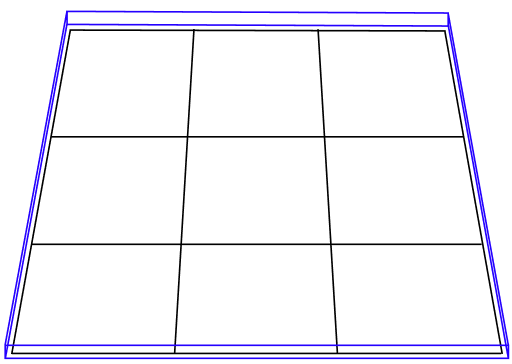
\includegraphics[width=\textwidth]{images/vorher.png}
        \caption{Begrenzungen vor Funktionsaufruf}
        \label{fig:vorher}
    \end{minipage}
    \hfill
    \begin{minipage}[b]{0.45\textwidth}
        \centering
        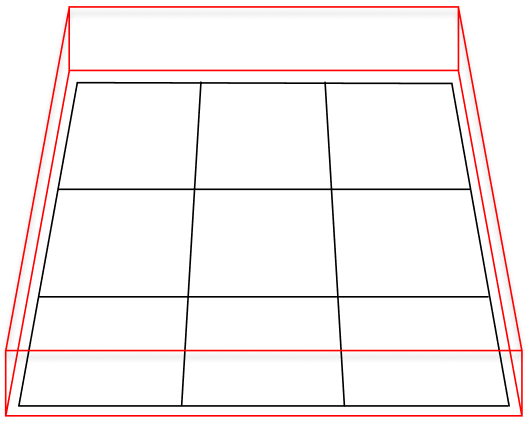
\includegraphics[width=\textwidth]{images/nachher.png}
        \caption{Begrenzungen nach Funktionsaufruf}
        \label{fig:nachher}
    \end{minipage}
\end{figure}

Die linke Abbildung \ref{fig:vorher} veranschaulicht deutlich die originalen und unveränderten Begrenzungen des Inventar
Objekts vor dem Aufruf der \texttt{UpdateInventoryBounds()} Funktion. Diese Begrenzungen geben an, welche Bereiche des
Inventars für die Erfassung von Gegenständen zugänglich sind.

Nach dem Aufruf der \texttt{UpdateInventoryBounds()} Funktion (siehe rechte Abbildung \ref{fig:nachher}) werden die Begrenzungen erweitert, um
sicherzustellen, dass alle relevanten Objekte ordnungsgemäß erfasst werden können. Dies ist entscheidend, um sicherzustellen,
dass das Inventarsystem effektiv funktioniert und dem Spieler eine nahtlose Erfahrung bietet.

Durch diesen Vorher-Nachher-Vergleich wird der positive Effekt der Funktion verdeutlicht. Sie trägt nicht nur zur Verbesserung
der Zuverlässigkeit des Inventarsystems bei, sondern steigert auch dessen Effizienz. Die erweiterten Begrenzungen ermöglichen
es dem Spieler, Gegenstände ohne Hindernisse oder Fehler hinzuzufügen oder zu entfernen, was letztendlich das Spielerlebnis
verbessert und den Spielfluss optimiert.

\subsubsection*{ID Grid Initialisierung}
Als letzter Schritt in der \texttt{Start()} Funktion erfolgt die Initialisierung des \texttt{idGrids}. Dieses zweidimensionale
Array dient dazu, die Gegenstände im Inventar zu verfolgen und ihre Positionen zu speichern. Es wird so dimensioniert,
dass es direkt die Größe des Inventarobjekts widerspiegelt und daher mit \texttt{numRows} und \texttt{numColumns}
initialisiert.
\begin{lstlisting}[style=csharp, caption={Initialisierung des idGrids}, label=code:controller_initialize]
private void InitializeIDGrid()
{
    idGrid = new int[numRows, numColumns];
}
\end{lstlisting}
Durch die Initialisierung des \texttt{idGrids} wird sichergestellt, dass das Inventarsystem die Positionen der Gegenstände
korrekt verfolgen und aktualisieren kann. Dies ist von entscheidender Bedeutung für die Interaktion des Benutzers mit dem
Inventar im weiteren Verlauf des Spiels.

\subsubsection*{Lokal- und Weltposition}
In Unity bezieht sich die \textit{lokale Position} eines Objekts auf seine Position relativ zu seinem Elternobjekt oder
zum Koordinatenursprung, wenn es kein Elternobjekt hat. Diese Position wird relativ zu den Achsen des Objekts selbst
angegeben, unabhängig von der umgebenden Szene.

Im Gegensatz dazu bezeichnet die \textit{Weltposition} eines Objekts seine Position im globalen Koordinatensystem der Szene.
Sie berücksichtigt die Position des Objekts relativ zum Koordinatenursprung der Szene sowie alle Transformationen, die
auf das Objekt angewendet wurden, einschließlich Verschiebung, Drehung und Skalierung.

Die Berechnung der Weltposition eines Objekts erfolgt durch Umrechnung seiner lokalen Position relativ zu seinem Elternobjekt
oder zum Koordinatenursprung in die Szene. Diese Berechnung wird durch eine einfache Vektoraddition realisiert, wobei die
lokale Koordinate des Objekts zur Weltkoordinate addiert wird, um die lokale Position in eine globale Koordinate umzuwandeln.
Dadurch wird die tatsächliche Position des Objekts in der Welt bestimmt, was Interaktionen mit anderen Objekten oder
Koordinaten in der Szene ermöglicht.

\subsubsection{Erkennen hinzugefügter oder entfernter Gegenstände}
Das Herzstück des \textit{InventoryController} bildet die Funktion \texttt{Update}. Sie trägt die Hauptverantwortung dafür,
neue Gegenstände innerhalb des Inventars zu erkennen und entfernte Gegenstände entsprechend zu entfernen. Darüber hinaus
gewährleistet sie, dass bei jedem Hinzufügen oder Entfernen eines Gegenstands das Inventar neu berechnet wird. Daraufhin
werden die drei \texttt{TextMeshes} innerhalb der \texttt{infoObjects} aktualisiert, um dem Benutzer stets die aktuellen
Inventarwerte und mögliche Fehlermeldungen anzuzeigen. Im Folgenden ist der Code dargestellt, der die Umsetzung dieser
Funktion verdeutlicht:
\begin{lstlisting}[style=csharp, caption={Neue / Entfernte Items erkennen}, label=code:controller_updateGrid]
void UpdateGrid()
{
    lock (activeQRObjects)
    {
        foreach (var item in activeQRObjects.Values)
        {
            QRCode qRCode = item.GetComponent<QRCode>();
            Vector3 worldPosition = item.transform.TransformPoint(qRCode.item.qrData.position);

            if (item != null && inventoryBounds.Contains(worldPosition))
            {
                int itemId = qRCode.item.qrData.id;

                if (!processedItems.Contains(itemId))
                {
                    if (currWeight + qRCode.item.qrData.weight <= cap)
                    {
                        userInfo.text = "";
                        processedItems.Add(itemId);
                        Vector2 startGridPosition = CalculateGridPosition(worldPosition);
                        idGrid[(int)startGridPosition.x, (int)startGridPosition.y] = itemId;
                        knapsackSolver?.UpdateInfoMesh("", Color.white);
                        currWeight += qRCode.item.qrData.weight;
                        EventManager.GridUpdate(idGrid);
                    }
                    else
                    {
                        knapsackSolver?.UpdateInfoMesh("Item hat zu viel Gewicht!", Color.red);
                    }
                }
            }
            else if (!inventoryBounds.Contains(worldPosition) && processedItems.Contains(qRCode.item.qrData.id) && ContainsId(qRCode.item.qrData.id))
            {
                int itemId = qRCode.item.qrData.id;
                processedItems.Remove(itemId);
                RemoveItem(itemId);
                currWeight -= qRCode.item.qrData.weight;
                EventManager.GridUpdate(idGrid);
            }
        }
    }
}
\end{lstlisting}
Im Wesentlichen kann die vorliegende Funktion in mehrere einzelne Schritte unterteilt werden, die den Verwaltungsvorgang
von neuen und entfernten Gegenstände steuert. Um diese Funktion dementsprechend Schritt für Schritt zu erklären, sind
hier die einzelnen Schritte samt Erklärung, was diese beinhalten beschrieben:
\begin{enumerate}
    \item \textbf{Sperren der aktiven QRCode Objekte}:
    Bevor die Verarbeitung der QRCode-Objekte beginnt, wird das Dictionary \texttt{activeQRObjects} gesperrt, um sicherzustellen,
    dass keine anderen Teile des Systems gleichzeitig darauf zugreifen und es möglicherweise inkonsistent machen können.

    \item \textbf{Iteration durch die QRCode-Objekte}:
    Innerhalb der gesperrten Region wird eine \texttt{foreach}-Schleife verwendet, um durch alle Werte des \texttt{activeQRObjects}
    Dictionaries zu iterieren. Jeder QRCode-Gegenstand wird einzeln überprüft und verarbeitet, um sicherzustellen, dass
    alle relevanten Aktionen auf jedes Element angewendet werden.

    \item \textbf{QRCode-Extraktion und Berechnung der Weltposition}:
    Diese Phase umfasst die Extraktion der QRCode-Komponente aus dem Gegenstandsobjekt und die darauf folgende Berechnung
    der Weltposition des Gegenstands. Hierbei wird die lokale Position des Gegenstands relativ zu seinem Elternelement
    transformiert, um seine exakte Position im globalen Koordinatensystem zu ermitteln. Die Funktionen \texttt{GetComponent<QRCode>()}
    und \texttt{TransformPoint()} werden dabei aufgerufen.

    \item \textbf{Überprüfung der Gegenstandspostition innerhalb der Inventargrenzen}:
    Ziel dieser Überprüfung ist es sicherzustellen, dass die berechnete Weltposition des Gegenstands innerhalb der
    festgelegten Grenzen des Inventars liegt. Nur Gegenstände, die sich innerhalb dieser Grenzen befinden, werden für das
    Inventar berücksichtigt. Es wird die Funktion \texttt{Contains()} aufgerufen, um zu prüfen, ob die Position innerhalb
    der Grenzen liegt.

    \item \textbf{Prüfung auf bereits erfolgte Verarbeitung des Gegenstands}:
    In diesem Schritt wird überwacht, ob der betreffende Gegenstand bereits im Inventar verarbeitet wurde, um doppelte
    Einträge zu verhindern und die Datenkonsistenz zu wahren. Die Funktion \texttt{Contains()} wird aufgerufen, um zu
    überprüfen, ob der Gegenstand bereits in der Liste der verarbeiteten Gegenstände enthalten ist.

    \item \textbf{Überprüfung des Gewichtslimits}:
    Diese Überprüfung dient dazu festzustellen, ob das Hinzufügen des Gegenstands das vorgegebene Gewichtslimit des
    Inventars überschreiten würde. Dadurch wird sichergestellt, dass das Inventar nicht überladen wird und das Gewichtslimit
    eingehalten wird. Hierbei wird die Funktion \texttt{UpdateInfoMesh()} aufgerufen, um das \texttt{InfoObject} zu aktualisieren.

    \item \textbf{Hinzufügen des Gegenstands zum Inventar}:
    Bei erfolgreicher Durchführung aller vorherigen Überprüfungen wird der Gegenstand zum Inventar hinzugefügt. Dies
    umfasst die Aktualisierung interner Datenstrukturen anhand der \texttt{CalculateGridPosition} Funktion, welche anhand
    der Weltposition des Gegenstands einen 2D-Vektor berechnet welcher die Position im Inventar repräsentiert, sowie des
    \texttt{InfoObjects}, um dem Benutzer die aktuellen Inventarinformationen bereitzustellen. Die Funktion \texttt{GridUpdate()}
    wird aufgerufen, um andere Teile des Systems über die Aktualisierung des Inventars zu informieren.

    \item \textbf{Anzeige einer Gewichtsüberschreitungsmeldung}:
    Falls das Hinzufügen des Gegenstands das Gewichtslimit überschreiten würde, erhält der Benutzer eine entsprechende
    Fehlermeldung, die ihn darauf hinweist, dass der Gegenstand nicht hinzugefügt werden kann, bis das Gewichtslimit
    eingehalten wird. Die Funktion \texttt{UpdateInfoMesh()} wird aufgerufen, um das \texttt{InfoObject} mit einer Fehlermeldung
    zu aktualisieren.

    \item \textbf{Überprüfung auf Gegenstandsaußerhalb-Liegen und Entfernung}:
    Hier wird anhand der \texttt{Contains()} und \texttt{ContainsId()} Funktionen geprüft, ob sich der Gegenstand außerhalb
    der definierten Inventargrenzen befindet. Sollte dies der Fall sein, wird der Gegenstand aus dem Inventar entfernt,
    um die Konsistenz und Integrität des Inventarsystems sicherzustellen. Die Funktionen \texttt{RemoveItem()} und \texttt{GridUpdate()}
    werden aufgerufen, um den Gegenstand zu entfernen und die Aktualisierung des Inventars zu signalisieren.
\end{enumerate}

\subsubsection{Zustände des Inventars aus der Sicht Benutzers}
In diesem Abschnitt werden die verschiedenen Zustände des Inventars aus Sicht des Benutzers anhand von Fallbeispielen
detailliert betrachtet. Das Inventar durchläuft unterschiedliche Zustände, darunter das Hinzufügen und Entfernen von
Gegenständen sowie das Überschreiten des Gewichtslimits. Es ist von großer Bedeutung, diese Zustände zu veranschaulichen,
um ein tieferes Verständnis für die Funktionsweise des Systems zu erlangen und dem Benutzer einen klaren Überblick zu
verschaffen. Jeder dieser Zustände wird durch visuelle Darstellungen illustriert, um zu veranschaulichen, wie sich das
Inventar sowie die zugrundeliegende Datenstruktur in verschiedenen Situationen verhalten. Dabei wird auch darauf eingegangen,
wie der Benutzer durch die grafische Benutzeroberfläche (GUI) über diese Zustände informiert wird.

\subsubsection*{Gegenstand zu dem Inventar hinzugefügt}
Dieser Zustand tritt ein, sobald der Benutzer einen Gegenstand erfolgreich an der Position 4 im Inventar platziert hat.
Das Inventar reagiert umgehend und integriert den neuen Gegenstand nahtlos in seine Struktur. Die nachfolgende Abbildung
\ref{fig:controller_itemAdded} visualisiert diesen Zustand.

\begin{figure}[H]
    \centering
    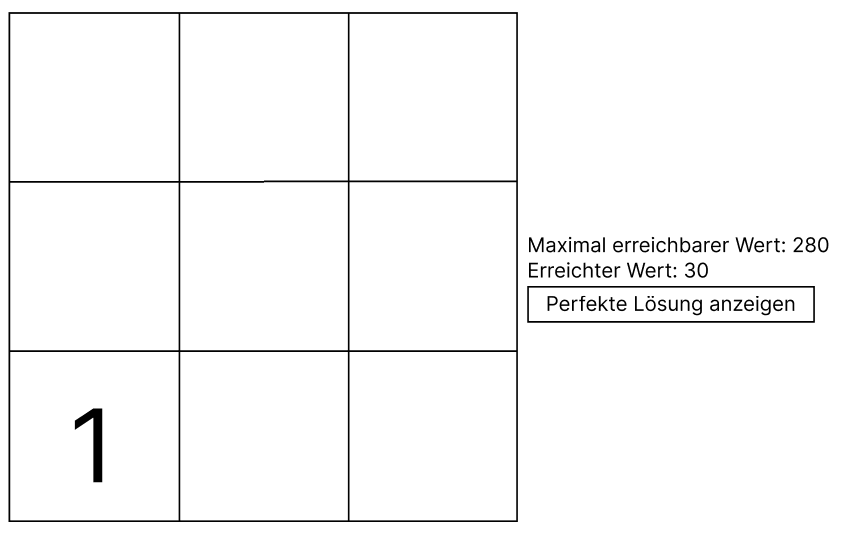
\includegraphics[scale=0.6]{images/itemAdded}
    \caption{Inventar mit erfolgreich hinzugefügtem Gegenstand}
    \label{fig:controller_itemAdded}
\end{figure}

Die Grafik verdeutlicht die gelungene Integration des neuen Gegenstands in das Inventar. Durch eine klare visuelle Darstellung
signalisiert das \texttt{infoMesh} dem Benutzer unmissverständlich den aktualisierten Zustand des Inventars und bestätigt
die erfolgreiche Platzierung des Gegenstands.

Im Hintergrund wird das \texttt{usedItems}-Array aktualisiert, um den neuen Gegenstand zu integrieren:
\[
    \text{usedItems} =
    \left[
        \begin{array}{ccccc}
            0 & 0 & 0 \\
            0 & 1 & 0 \\
            0 & 0 & 0 \\
        \end{array}
        \right]
\]

Gleichzeitig wird der Gegenstand in das \texttt{processedItems}-Array aufgenommen, um sicherzustellen, dass er nicht
doppelt berücksichtigt wird:
\[
    \text{processedItems} = \{1\}
\]

\subsubsection*{Gegenstand aus dem Inventar entfernt}
Dieser Zustand tritt ein, sobald der Benutzer einen Gegenstand aus dem Inventar entfernt hat, wie in Abbildung \ref{fig:controller_itemRemoved}
dargestellt.

\begin{figure}[H]
    \centering
    \includegraphics[scale=0.6]{images/itemRemoved}
    \caption{Inventar nach Entfernen eines Gegenstands}
    \label{fig:controller_itemRemoved}
\end{figure}

Die Grafik zeigt das Inventar nach Entfernen des Gegenstands aus der Position 4. Das \texttt{infoMesh} signalisiert dem
Benutzer deutlich den aktualisierten Zustand des Inventars und bestätigt die erfolgreiche Entfernung des Gegenstands.

Im Hintergrund wird das \texttt{usedItems}-Array aktualisiert, um den entfernten Gegenstand zu berücksichtigen:
\[
    \text{usedItems(vorher)} =
    \left[
        \begin{array}{ccccc}
            0 & 0 & 0 \\
            0 & 1 & 0 \\
            0 & 0 & 0 \\
        \end{array}
        \right]
\]

\[
    \text{usedItems(nachher)} =
    \left[
        \begin{array}{ccccc}
            0 & 0 & 0 \\
            0 & 0 & 0 \\
            0 & 0 & 0 \\
        \end{array}
        \right]
\]

Gleichzeitig wird der Gegenstand aus dem \texttt{processedItems}-Array entfernt, um sicherzustellen, dass er nicht erneut
verarbeitet wird:
\[
    \text{processedItems (vorher)} = \{1\}
\]

\[
    \text{processedItems (nachher)} = \{\}
\]

\subsubsection*{Gegenstand zu schwer für das Inventar}
Dieser Zustand tritt ein, wenn der Benutzer versucht, einen Gegenstand hinzuzufügen, der das Gewichtslimit des Inventars
überschreitet, wie in Abbildung \ref{fig:controller_itemTooHeavy} illustriert.

\begin{figure}[H]
    \centering
    \includegraphics[scale=0.6]{images/itemTooHeavy}
    \caption{Inventar mit einem Gegenstand, der das Gewichtslimit überschreitet}
    \label{fig:controller_itemTooHeavy}
\end{figure}

Die Grafik zeigt das Inventar mit mehreren hinzugefügten Gegenständen. Die Reihenfolge in der diese Gegenstände hinzugefügt
wurden, ist die folgende: 1, 5, 3, 9. Die ist wichtig, weil der letzte hinzugefügt Gegenstand den zu schweren Gegenstand
widerspiegelt. Auch zu sehen ist, dass das \texttt{infoMesh} den Benutzer deutlich über das Überschreiten des Gewichtslimits
informiert und das Hinzufügen des Gegenstands verhindert.

Im Hintergrund bleibt das \texttt{usedItems}-Array unverändert, da der Gegenstand nicht hinzugefügt wurde:
\[
    \text{usedItems} =
    \left[
        \begin{array}{ccccc}
            0 & 0 & 0 \\
            1 & 0 & 0 \\
            5 & 3 & 0 \\
        \end{array}
        \right]
\]

Das \texttt{processedItems}-Array bleibt ebenfalls unverändert:
\[
    \text{processedItems} = \{1, 5, 3\}
\]

\subsection{EventManager} \marginpar{\small\(\rightarrow\) HAYLAZ}

Der \textit{EventManager} ist ein entscheidendes Game-Objekt, das als zentrales Kommunikationselement fungiert und die
Interaktion zwischen verschiedenen Komponenten und Klassen innerhalb der Anwendung ermöglicht. Implementiert als Klasse
im Skript \textit{EventManager.cs}, das dem Game-Objekt angehängt ist, spielt er eine unverzichtbare Rolle trotz seiner
Kompaktheit, da er die Schnittstelle für die Kommunikation zwischen verschiedenen Klassen und Game-Objekten bereitstellt.

Das Konzept der Ereignisse ermöglicht die Kommunikation zwischen verschiedenen Teilen eines Programms, ohne dass direkte
Abhängigkeiten zwischen diesen Teilen bestehen müssen. Andere Teile des Codes können sich auf diese Ereignisse registrieren,
um benachrichtigt zu werden, wenn sie auftreten. In diesem Zusammenhang werden spezifische Ereignisse definiert:

\begin{itemize}
\item \textbf{Nachrichteneingang}: Dieses event wird ausgelöst, wenn im ersten Level eine Nachricht von einem Laptop
empfangen wird. Nach dem Auslösen wird ein Ping-Paket über ein Kabel auf der Brille simuliert.
\item \textbf{Nachricht versendet}: Dieses Event wird ausgelöst, wenn im ersten Level eine Nachricht an einen Laptop
gesendet wird. Es dient dazu die Empfangene Nachricht an das zweite Laptop im richtigen Moment (nach Abschluss der
Simulation) weiter zu leiten.
\item \textbf{Inventar Aktualisierung}: Dieses Event wird ausgelöst, wenn im zweiten Level ein Item ins Inventar gelegt und
das Inventar aktualisiert wird. Nach der Aktualisierung wird der aktuelle Wert des Inventars berechnet. Dadurch können
wir auf eine ständige Neuberechnung des Inventars verzichten und limitierte Ressourcen sparen.
\end{itemize}

Die Klasse \textit{EventManager} definiert diese Ereignisse als statische Ereignisse und stellt Methoden bereit, um die
Ereignisse auszulösen. Dies erleichtert die globale Verwendung des Ereignissystems in verschiedenen Teilen des Codes.
Die Aktionen (Actions) sind statisch, was bedeutet, dass sie auf Klassenebene definiert sind und keine Instanz der Klasse
benötigen, um aufgerufen zu werden. Die Methode \textit{Invoke} wird verwendet, um die Ereignisse auszulösen.

\begin{lstlisting}[style=csharp, label=code:EventManager]
public static class EventManager
{
    // Level 1
    public static event System.Action<int, string, string> OnMessageReceived;
    public static void ReceiveMsg(int idx, string username, string message) => OnMessageReceived?.Invoke(idx, username, message);

    public static event System.Action<int, string, string> OnMessageSend;
    public static void SendMsg(int idx, string username, string message) => OnMessageSend?.Invoke(idx, username, message);

    // Level 2
    public static event System.Action<int[,]> OnGridUpdate;
    public static void GridUpdate(int[,] grid) => OnGridUpdate?.Invoke(grid);
}
\end{lstlisting}

Das ist die definition der Ereignisse und Methoden, die verwendet werden, um die Ereignisse auszulösen.
Um auf diese Ereignisse zu reagieren, können andere Teile des Codes sich auf diese Ereignisse registrieren, welches wie folgend
aussieht:

\begin{lstlisting}[style=csharp label=code:Event Registration]
//Dieser Code Abschnitt befindet sich in der Klasse: KnapsackSolver.cs

void Start()
{
    items = new QRItem(0).items;
    EventManager.OnGridUpdate += SetInventory;
}

public void SetInventory(int[,] newInventory)
{
    inventory = newInventory;
    CalculateKnapsack();
}
\end{lstlisting}

Nach laden der Scene registriert sich die \textit{KnapsackSolver} Klasse auf das \textit{OnGridUpdate} Event mit
der \textit{setInventory} Methode. Dies bedeutet, dass jedes mal wenn das \textit{OnGridUpdate} Event ausgelöst wird,
die \textit{setInventory} Methode aufgerufen wird und der aktuelle Wert des neuen Inventars berechnet wird.

\begin{lstlisting}[style=csharp label=code:Event Trigger]
EventManager.GridUpdate(idGrid);
\end{lstlisting}

Das auslösen des \textit{OnGridUpdate} Events wird durch den obigen Codeabschnitt erreicht. Dieser Codeabschnitt befindet
sich in der \textit{InventoryController} Klasse und wird aufgerufen, wenn ein neues Item hinzugefügt oder entfernt wird.

Insgesamt ermöglicht dieser simple Code eine lose Kopplung zwischen verschiedenen Teilen des Programms, indem Ereignisse verwendet
werden, um auf bestimmte Aktionen zu reagieren, ohne dass die beteiligten Teile voneinander wissen müssen. Dadurch wird die
Modularität, Erweiterbarkeit und Wartbarkeit der Anwendung gefördert.

\subsection{Das Knapsack Problem} \marginpar{\small\(\rightarrow\) SKREPEK}
Dieser Abschnitt befasst sich mit allem Rund um das Thema des bekannten Optimierungsproblems des Knapsack-Problems, die
Problemstellung, welche Varianten und Typen des Problems es gibt, die zwei bekanntesten Algorithmen zum Lösen des Problems
und anschließend die Implementierung um das Problem zu lösen.

\subsubsection{Knapsack-Algorithmus}
Der Knapsack-Algorithmus ist ein grundlegendes Werkzeug in der Informatik, das sich mit der optimalen Ressourcenallokation
beschäftigt, insbesondere wenn es darum geht, eine begrenzte Menge an Ressourcen effizient zu nutzen, um einen bestimmten
Nutzen oder Gewinn zu maximieren. Die Metapher des \textit{Knapsacks} bezieht sich dabei auf die Vorstellung, einen Rucksack
mit einer begrenzten Kapazität zu füllen, wobei die enthaltenen Gegenstände jeweils unterschiedliche Werte und Gewichte aufweisen.

\subsubsection{Problemstellung}
Das Knapsack-Problem befasst sich mit der Herausforderung, einen Rucksack optimal zu befüllen, wenn dieser eine begrenzte
Kapazität aufweist. Um diesen zu füllen, stehen hier eine Reihe von Gegenständen zur Auswahl, von denen jeder einen
individuellen Wert, der einen bestimmten Nutzen oder eine Wichtigkeit repräsentiert. Auch hat jeder Gegenstand ein
bestimmtes individuelles Gewicht, welches genau beschreibt, wie viel an Platz dieser Gegenstand im Rucksack einnimmt.

Das grundlegende Ziel beim Knapsack-Problem besteht darin, eine Auswahl von Gegenständen zu treffen, die in den Rucksack
passt und gleichzeitig den Gesamtwert der ausgewählten Gegenstände maximiert. Dabei muss die Summe der Gewichte der
ausgewählten Gegenstände die Kapazität des Rucksacks nicht überschreiten. Dies führt zu einer Herausforderung, bei der
eine perfekte Lösung gefunden werden muss, um den bestmöglichen Nutzen aus den verfügbaren Gegenständen zu ziehen.

\subsubsection{Variationen des Knapsack-Problems}
Im Laufe der Zeit hat das Knapsack-Problem verschiedene Variationen hervorgebracht, die jeweils unterschiedliche Aspekte
und Einschränkungen des Problems berücksichtigen. Nachfolgend werden einige bekannte Variationen erläutert.

\subsubsection*{Mehrzieliges Knapsack-Problem}
Das mehrzielige Knapsack-Problem erweitert das klassische Knapsack-Problem, indem es \textit{mehrere Zielkriterien}
berücksichtigt. Anstatt nur den Gesamtwert der ausgewählten Gegenstände zu maximieren, sollen nun mehrere Ziele \textit{gleichzeitig optimiert}
werden. Zum Beispiel könnte neben der \textit{Maximierung} des Gesamtwerts auch die \textit{Minimierung} des Gesamtgewichts
oder anderer Kosten angestrebt werden. Diese Variation des Problems führt zu komplexeren Optimierungsaufgaben, da
Kompromisse zwischen den verschiedenen Zielen gefunden werden müssen.

\subsubsection*{Multidimensionales Knapsack-Problem}
Beim multidimensionalen Knapsack-Problem hat jeder Gegenstand nicht nur ein Gewicht, sondern wird durch einen \textit{M-dimensionalen}
Vektor repräsentiert, der verschiedene \textit{Merkmale} oder \textit{Eigenschaften} des Gegenstands darstellt. Entsprechend
ist auch die Kapazität des Rucksacks ein \textit{M-dimensionaler} Vektor. Diese Variation des Problems entsteht häufig
in realen Anwendungen, in denen die Gegenstände durch mehrere Merkmale charakterisiert werden, wie zum Beispiel \texit{Größe},
\textit{Form}, \textit{Farbe} oder \textit{Material}.

\subsubsection*{Mehrere Knapsack-Probleme}
Das multiple Knapsack-Problem \textit{erweitert} das klassische Knapsack-Problem, indem es mehrere Rucksäcke oder Behälter
einführt, in die die Gegenstände verteilt werden können. Im Gegensatz zum klassischen Problem, bei dem alle Gegenstände in
einen einzelnen Rucksack gepackt werden müssen, können hier mehrere Rucksäcke genutzt werden, um die Gegenstände aufzunehmen.
Diese Variation ist relevant in Situationen, in denen die Gegenstände auf verschiedene Weise organisiert oder verwendet
werden sollen.

\subsubsection*{Quadratisches Knapsack-Problem}
Das quadratische Knapsack-Problem bezieht sich auf eine Variation, bei der das Ziel darin besteht, eine quadratische
Zielfunktion zu maximieren, die von den ausgewählten Gegenständen abhängt. Diese Zielfunktion kann beispielsweise den
Gesamtnutzen oder den Gesamtwert der ausgewählten Gegenstände darstellen und ist oft von quadratischer Form in Bezug auf
die Variablen, die die Auswahl der Gegenstände repräsentieren. Die Lösung dieses Problems erfordert spezielle Techniken
zur Bewältigung der quadratischen Struktur der Zielfunktion.

\subsubsection*{Geometrisches Knapsack-Problem}
Beim geometrischen Knapsack-Problem stehen eine Reihe von geometrischen Objekten mit unterschiedlichen \textit{Formen}
und \textit{Größen} zur Auswahl, die in einen \textit{rechteckigen Rucksack} gepackt werden sollen. Das Ziel besteht darin,
die Gegenstände so anzuordnen, dass der verfügbare Platz im Rucksack optimal genutzt wird und der Gesamtwert der
ausgewählten Gegenstände maximiert wird. Diese Variation des Knapsack-Problems erfordert eine \textit{Berücksichtigung}
der \textit{geometrischen Eigenschaften} der Objekte und kann in verschiedenen Anwendungen wie Layoutdesign oder Packungsproblemen
auftreten.\footnote{GeeksForGeeks, \cite{Introduction to Knapsack Problem, its Types and How to solve them}}

\subsubsection{Typen des Knapsack-Problems}
Das Knapsack-Problem kann in verschiedene Typen unterteilt werden, die jeweils \textit{unterschiedliche Bedingungen} und
\textit{Anforderungen} haben. Nachfolgend werden die wichtigsten Typen des Knapsack-Problems erläutert.

\subsubsection*{0/1 Knapsack-Problem}
Das 0/1-Knapsack-Problem bezieht sich auf die effiziente Auswahl von Gegenständen, um den maximalen Gesamtwert in einem
begrenzten Rucksack zu erreichen. Gegeben sind \textit{N Gegenstände}, wobei jedem Gegenstand ein bestimmtes Gewicht
(\textit{w}) und ein Wert (\textit{v}) zugeordnet ist. Außerdem steht ein Rucksack mit einer Kapazität (\textit{C}) zur
Verfügung. Das Ziel besteht darin, die Gegenstände in den Rucksack zu legen, sodass die Summe der Werte der ausgewählten
Gegenstände maximal ist.

Es ist wichtig zu beachten, dass beim 0/1-Knapsack-Problem entweder ein Gegenstand \textit{vollständig} in den Rucksack
gepackt wird oder \textit{überhaupt nicht}. Es gibt \textit{keine Möglichkeit}, einen Gegenstand \textit{teilweise} in
den Rucksack zu legen. Diese Beschränkung erfordert eine sorgfältige Auswahl der Gegenstände, um den verfügbaren Platz
im Rucksack optimal zu nutzen und gleichzeitig den Gesamtwert zu maximieren.

\subsubsection*{Fraktionales Knapsack-Problem}
Das fraktionale Knapsack-Problem befasst sich mit der effizienten Verteilung von Gegenständen in einem Rucksack, um den
Gesamtwert im Rucksack zu maximieren. Dabei werden die Gewichte und Werte von \textit{N Gegenständen} gegeben, und das
Ziel besteht darin, diese Gegenstände in einen Rucksack mit der \textit{Kapazität W} zu legen, um den maximalen Gesamtwert
zu erreichen. Im Gegensatz zum klassischen 0/1-Knapsack-Problem, bei dem entweder ein Gegenstand vollständig in den
Rucksack gepackt wird oder nicht, erlaubt das fraktionale Knapsack-Problem das Aufteilen von Gegenständen, um den Gesamtwert
im Rucksack zu maximieren. Diese Flexibilität ermöglicht es, eine perfekte Lösung zu finden, indem die Gegenstände
entsprechend ihrer Wertigkeit und Gewichtung effizient verteilt werden.

\subsubsection*{Begrenztes Knapsack-Problem}
Das begrenzte Knapsack-Problem bezieht sich auf die effiziente Auswahl von Gegenständen, um den maximalen Gesamtwert unter
Berücksichtigung eines begrenzten Gewichts zu erreichen. Angenommen, es gibt \textit{N Gegenstände}, wobei jedem Gegenstand
ein bestimmtes Gewicht (\textit{w}) und ein Wert (\textit{v}) zugeordnet ist. Die Aufgabe besteht darin, den Gesamtwert
zu maximieren, indem maximal \textit{N Gegenstände} ausgewählt werden, deren Gesamtgewicht nicht größer als das maximale
Gewicht \textit{W} ist.

\subsubsection*{Unbegrenztes Knapsack-Problem}
Das unbeschränkte Knapsack-Problem befasst sich mit der effizienten Auswahl von Gegenständen, um den maximalen Gesamtwert
zu erreichen, wobei das Gesamtgewicht nicht größer als eine vorgegebene Kapazität ist. Angenommen, es gibt ein
Rucksackgewicht \textit{W} und eine Menge von \textit{N Gegenständen}, von denen jeder einen bestimmten Wert (\textit{v})
und ein Gewicht (\textit{w}) hat. Das Ziel besteht darin, die maximale Menge zu berechnen, die genau dieses Gewicht
erreichen kann.

Im Gegensatz zum 0/1-Knapsack-Problem, bei dem die Anzahl der Instanzen eines Gegenstands begrenzt ist, können beim
unbeschränkten Knapsack-Problem \textit{beliebig viele} Instanzen \textit{desselben} Gegenstands verwendet werden. Dies
ermöglicht eine flexiblere Auswahl und Nutzung der verfügbaren Gegenstände, um den maximalen Gesamtwert zu erzielen, der
das vorgegebene Gewicht nicht überschreitet.\footnote{GeeksForGeeks, \cite{Introduction to Knapsack Problem, its Types and How to solve them}}

\subsubsection{Ansätze zur Lösung des Knapsack-Problems}
Das Knapsack-Problem bietet Raum für eine Vielzahl von Lösungsansätzen, die sich in ihrer \textit{Komplexität}, \textit{Effizienz}
und \textit{Genauigkeit} unterscheiden können. Diese Ansätze reichen von einfachen \textit{heuristischen Methoden} bis
hin zu \textit{komplexen optimierten Algorithmen}. Abgesehen von \textit{dynamischer Programmierung} und dem \textit{Greedy-Ansatz},
die später genauer betrachtet werden, gibt es weitere interessante Möglichkeiten, das Knapsack-Problem anzugehen.

Ein Ansatz besteht darin, das Problem in kleinere Teilprobleme zu zerlegen und diese dann unabhängig voneinander zu lösen.
Durch die Kombination der Lösungen dieser Teilprobleme kann eine Gesamtlösung gefunden werden. Diese Methode ist besonders
nützlich, wenn die Problemgröße groß ist und eine vollständige Suche nach einer optimalen Lösung zu aufwändig ist.

Eine weitere Herangehensweise ist die Verwendung von \textit{Metaheuristiken}, wie etwa \textit{genetische Algorithmen}
oder \textit{Schwarmintelligenz}. Diese Algorithmen basieren auf biologischen oder sozialen Konzepten und verwenden
probabilistische Techniken, um Lösungen zu finden, die möglicherweise nicht optimal, aber dennoch akzeptabel sind. Sie
eignen sich gut für komplexe Probleme, bei denen eine exakte Lösung schwer zu erreichen ist.

Eine neuere Entwicklung in der Lösung des Knapsack-Problems ist der Einsatz von \textit{maschinellem Lernen} und \textit{künstlicher Intelligenz}.
Durch den Einsatz von \textit{Datenanalyse} und \textit{statistischen Methoden} können Modelle trainiert werden, um Muster
in den Eigenschaften der Gegenstände und den Anforderungen des Rucksacks zu erkennen und optimale Packstrategien vorherzusagen.

\subsubsection*{Dynamischer Programmieransatz genauer betrachtet}
Der dynamische Programmieransatz ist eine leistungsfähige Methode zur Lösung des Knapsack-Problems, die auf der Idee beruht,
das Problem in kleinere Teilprobleme zu zerlegen und die Lösungen dieser Teilprobleme systematisch zu kombinieren, um die
optimale Gesamtlösung zu finden. Diese Methode eignet sich besonders gut für Probleme, bei denen Teilprobleme sich überlappen
und dieselben Teillösungen verwendet werden können, um mehrere Teilprobleme zu lösen.

Der folgende Pseudocode veranschaulicht den dynamischen Algorithmus zur Lösung des Knapsack-Problems:
\begin{lstlisting}[style=csharp, caption={Dynamischer Algorithmus}]
FUNCTION knapsackDynamic(weights[], values[], capacity)
    n = length(weights)
    DECLARE Tabelle[n + 1][capacity + 1]
    FOR i FROM 0 TO n DO
        FOR w FROM 0 TO capacity DO
            IF i == 0 OR w == 0 THEN
                Tabelle[i][w] = 0
            ELSE IF weights[i-1] <= w THEN
                Tabelle[i][w] = MAX(values[i-1] + Tabelle[i-1][w - weights[i-1]], Tabelle[i-1][w])
            ELSE
                Tabelle[i][w] = Tabelle[i-1][w]
            END IF
        END FOR
    END FOR
    RETURN Tabelle[n][capacity]
END FUNCTION
\end{lstlisting}\\
\\
Die Funktion \textbf{knapsackDynamic} implementiert den dynamischen Programmieransatz zur Lösung des Knapsack-Problems.
Sie akzeptiert drei Parameter: ein Array von Gewichten (\( \textit{weights} \)), ein Array von Werten (\( \textit{values} \))
und die Kapazität des Rucksacks (\( \textit{capacity} \)).

Zuerst wird die Länge des Gewichtsarrays \( \textit{n} \) berechnet, um die Anzahl der verfügbaren Gegenstände zu bestimmen.
Dann wird eine Tabelle \( \textit{Tabelle} \) mit \( \textit{n+1} \) Zeilen und \( \textit{capacity+1} \) Spalten initialisiert.
Diese Tabelle dient dazu, die optimalen Werte für verschiedene Teilprobleme zu speichern.

Anschließend werden zwei verschachtelte Schleifen verwendet, um alle möglichen Kombinationen von Gegenständen und Gewichten
zu durchlaufen. Dabei wird für jedes Teilproblem in der Tabelle der optimale Wert berechnet. Die innere Schleife iteriert
über die möglichen Kapazitäten des Rucksacks, während die äußere Schleife die verfügbaren Gegenstände durchläuft.

Für jedes Teilproblem wird überprüft, ob der aktuelle Gegenstand in den Rucksack passt. Wenn ja, wird der Wert dieses
Gegenstands zu dem Wert addiert, der erreicht werden kann, wenn der Rucksack ohne diesen Gegenstand gefüllt wird. Andernfalls
wird der Wert aus der vorherigen Zeile der Tabelle übernommen, da der aktuelle Gegenstand nicht in den Rucksack passt.

Schließlich wird der Wert in der untersten rechten Zelle der Tabelle zurückgegeben, der den maximal erreichbaren Gesamtwert
des Rucksacks darstellt.

Dieser Algorithmus nutzt die Eigenschaften der optimalen Teilstruktur und des Überlappungsprinzips aus, um eine effiziente
Lösung des Knapsack-Problems zu finden. Durch die systematische Berechnung und Speicherung der optimalen Werte für Teilprobleme
ermöglicht der dynamische Programmieransatz eine Zeitkomplexität von \( O(n \cdot capacity) \), was für viele praktische
Anwendungen akzeptabel ist.

\subsubsection*{Aufbau und Interpretation der Tabelle der Teilprobleme}
Die Tabelle der Teilprobleme spielt eine entscheidende Rolle bei der systematischen Lösung des Knapsack-Problems mithilfe
des dynamischen Programmieransatzes. Sie ist eine zweidimensionale Matrix, die während des Algorithmusverlaufs generiert
wird und die optimalen Lösungen für verschiedene Teilprobleme des Knapsack-Problems enthält. Die Matrix ist wie folgt strukturiert:

\[
\left[
\begin{array}{ccccc}
a_{11} & a_{12} & a_{13} & \cdots & a_{1n} \\
a_{21} & a_{22} & a_{23} & \cdots & a_{2n} \\
a_{31} & a_{32} & a_{33} & \cdots & a_{3n} \\
a_{31} & a_{32} & a_{33} & \cdots & a_{3n} \\
\vdots & \vdots & \vdots & \ddots & \vdots \\
a_{m1} & a_{m2} & a_{m3} & \cdots & a_{mn} \\
\end{array}
\right]
\]

Jede \textit{Zeile} in der Matrix entspricht den verschiedenen verfügbaren Gewichtskapazitäten des Rucksacks, beginnend
bei \textit{null} und schrittweise bis zur \textit{maximalen Kapazität}.

Jede \textit{Spalte} in der Matrix repräsentiert die Anzahl der bereits \textit{berücksichtigten Gegenstände}, wobei jede
Spalte die \textit{Teilprobleme} für eine zunehmende Anzahl von Gegenständen darstellt.\\
\\
Um anschließend eine Zelle \( a_{mn} \) dieser Matrix zu interpretieren, ist Folgendes wichtig zu wissen:
\begin{enumerate}
\item \textbf{m} gibt an, wie viel \textit{Gewicht} bereits im Rucksack verbraucht wurde. Je weiter fortgeschritten dieser
Wert ist, daher desto weiter unten in der Tabelle und desto mehr Gewicht wurde bereits verwendet.
\item \textbf{n} gibt an, wie viele \textit{Gegenstände} bereits betrachtet wurden. Je weiter fortgeschritten, daher,
desto weiter rechts in der Tabelle und desto mehr Gegenstände wurden bereits berücksichtigt.
\end{enumerate}

Die Einträge in der Matrix werden durch den \textit{dynamischen Programmieransatz} berechnet, indem die optimalen Werte für
Teilprobleme \textit{schrittweise kombiniert} werden, um den Wert für größere Teilprobleme zu bestimmen.

\subsubsection*{Greedy-Ansatz genauer betrachtet}
Im Gegensatz zur dynamischen Lösung wählt der Greedy-Ansatz Gegenstände basierend auf bestimmten Kriterien aus, um eine
lokale Optimierung zu erreichen. Hierbei wird in jedem Schritt diejenige Entscheidung getroffen, die im Moment am
vorteilhaftesten erscheint, ohne jedoch die Gesamtoptimierung im Auge zu behalten.

Der folgende Pseudocode veranschaulicht den Greedy-Algorithmus zur Lösung des Knapsack-Problems:

\begin{lstlisting}[style=csharp, caption={Greedy Algorithmus}]
FUNCTION knapsackGreedy(weights[], values[], capacity)
    n = length(weights)
    DECLARE items[n]
    FOR i FROM 0 TO n DO
        items[i] = (values[i] / weights[i], weights[i], values[i])
    END FOR
    SORT items by ratio in descending order
    totalValue = 0
    currentWeight = 0
    FOR i FROM 0 TO n DO
        IF currentWeight + items[i].weight <= capacity THEN
            currentWeight += items[i].weight
            totalValue += items[i].value
        ELSE
            ratio = (capacity - currentWeight) / items[i].weight
            totalValue += ratio * items[i].value
            BREAK
        END IF
    END FOR
    RETURN totalValue
END FUNCTION
\end{lstlisting}\\
Die Funktion \textbf{knapsackGreedy()} nimmt wie der dynamische Ansatz drei Parameter an: ein Array von Gewichten (\( \textit{weights} \)),
ein Array von Werten (\( \textit{values} \)) und die Kapazität des Rucksacks (\( \textit{capacity} \)). Die Funktionsweise
dieses Ansatzes ist wie folgt:

\begin{enumerate}
\item Zunächst wird für jeden Gegenstand das Verhältnis von Wert zu Gewicht berechnet und in einer Liste von Tupeln
gespeichert. Jedes Tupel enthält das Wert-Gewichts-Verhältnis sowie das Gewicht und den Wert des entsprechenden Gegenstands.
\item Die Liste der Gegenstände wird basierend auf dem Verhältnis von Wert zu Gewicht in absteigender Reihenfolge
sortiert, um die Gegenstände mit dem höchsten Verhältnis zuerst zu betrachten.
\item Der Algorithmus durchläuft die sortierte Liste der Gegenstände und versucht, jeden Gegenstand dem Rucksack
hinzuzufügen. Dabei wird überprüft, ob das Hinzufügen des Gegenstands das Gewichtslimit des Rucksacks überschreitet.
Falls dies der Fall ist, wird ein Teil des Gegenstands entsprechend dem verbleibenden verfügbaren Gewicht im Rucksack hinzugefügt.
\item Nachdem alle Gegenstände überprüft wurden, wird der Gesamtwert der im Rucksack enthaltenen Gegenstände zurückgegeben.
Dies stellt die Lösung des Problems dar.
\end{enumerate}

Der Greedy-Algorithmus bietet eine einfache und effiziente Lösung für das Knapsack-Problem, die jedoch nicht immer die
perfekte Lösung garantiert. Durch die Auswahl der Gegenstände basierend auf lokalen Kriterien kann der Algorithmus zu
suboptimalen Ergebnissen führen, insbesondere wenn die Gegenstände stark voneinander abhängen oder das Gewichtslimit des
Rucksacks sehr restriktiv ist.

\subsubsection{Anwendungen des Knapsack-Problems}
Die grundlegende Problemstellung des Knapsack-Problems hat breite Anwendung in verschiedenen \textit{wissenschaftlichen}
und \textit{industriellen} Bereichen gefunden und bildet die Grundlage für eine Vielzahl von Algorithmen und Anwendungen.

Dieses Kapitel untersucht die Anwendungen des Knapsack-Problems und seine Bedeutung in verschiedenen Domänen. Von der
\textit{Logistik} über die \textit{Finanzplanung} bis hin zum \textit{Ressourcenmanagement} und der \textit{Netzwerkoptimierung}
hat das Knapsack-Problem einen entscheidenden Einfluss auf die moderne Technologie und Wirtschaft.

Die Anwendungen des Knapsack-Problems lassen sich in vier Hauptbereiche unterteilen:
\begin{enumerate}
\item \textbf{Logistik}: Der Knapsack-Algorithmus wird in der Logistik angewendet, um den Transport von Gütern mit
begrenzten Kapazitäten zu optimieren. Indem er die bestmögliche Auswahl von Gütern trifft, ermöglicht er Logistikunternehmen,
ihre Transportkosten zu minimieren und die Effizienz ihrer Lieferketten zu steigern. Dies kann die Planung von LKW-Routen,
die Beladung von Containern oder die Organisation von Waren in Lagern umfassen.
\item \textbf{Finanzplanung}: In der Finanzplanung wird der Knapsack-Algorithmus genutzt, um Portfolios von Investitionen
zu optimieren. Investoren können mithilfe dieses Algorithmus eine Auswahl von Wertpapieren treffen, die das Risiko
minimieren und den erwarteten Ertrag maximieren. Dies kann die Diversifizierung von Anlagen, die Auswahl von Aktien
oder die Verwaltung von Fonds umfassen.
\item \textbf{Ressourcenmanagement}: Der Knapsack-Algorithmus wird im Ressourcenmanagement verwendet, um die effiziente
Nutzung begrenzter Ressourcen sicherzustellen. Dies kann in der Produktion erfolgen, wo Arbeitskräfte, Maschinen und
Materialien effizient zugewiesen werden müssen, oder im Projektmanagement, um Zeit und Budgets zu optimieren. Durch
die Anwendung des Knapsack-Problems können Unternehmen ihre Produktivität steigern und Kosten senken.
\item \textbf{Netzwerkoptimierung}: In der Netzwerkoptimierung spielt der Knapsack-Algorithmus eine wichtige Rolle
bei der Planung und Optimierung von verschiedenen Arten von Netzwerken. Dies kann die Optimierung von Transportrouten,
die Verteilung von Ressourcen in Computernetzwerken oder die Verbesserung der Bandbreitenauslastung in Telekommunikationsnetzen
umfassen. Der Einsatz des Knapsack-Problems ermöglicht es, die Leistung von Netzwerken zu verbessern und Engpässe zu
minimieren.\footnote{GeeksForGeeks, \cite{Introduction to Knapsack Problem, its Types and How to solve them}}
\end{enumerate}

Die Untersuchung dieser Anwendungen veranschaulicht die Vielseitigkeit und Effektivität des Knapsack-Problems bei der Lösung
komplexer Optimierungsprobleme. Darüber hinaus trägt die Anwendung des Knapsack-Algorithmus dazu bei, industrielle Abläufe
zu verbessern, Kosten zu senken und die Effizienz in verschiedenen Bereichen zu steigern.

\subsubsection{Auswahl des Implementierungsansatzes}
Die Wahl des Implementierungsansatzes für den Knapsack-Algorithmus in dieser Anwendung ist von entscheidender Bedeutung
für den Erfolg des Projekts. Moderne Softwaresysteme stehen vor einer Vielzahl von Herausforderungen und Anforderungen,
die eine sorgfältige Auswahl eines geeigneten Algorithmus erforderlich machen.

Die Entscheidung für den Implementierungsansatz erfolgte nach einer eingehenden Analyse der Anforderungen der Anwendung
und einer gründlichen Untersuchung der verfügbaren Algorithmen sowie ihrer Eigenschaften. Dabei wurden verschiedene
Faktoren berücksichtigt, darunter die Notwendigkeit einer optimalen Lösung, die Effizienz der Algorithmusausführung, die
Flexibilität in Bezug auf unterschiedliche Problemvarianten und die Genauigkeit der berechneten Ergebnisse.

Diese überlegungen werden anschließend ausführlich diskutiert und die Gründe für die Wahl des dynamischen Ansatzes als
Implementierungsstragie für den Knapsack-Algorithmus erläutert:
\begin{enumerate}
\item \textbf{Perfekte Lösungsgarantie}: Der dynamische Ansatz bietet die Möglichkeit, eine perfekte Lösung für das
Knapsack-Problem zu garantieren. Dies ist besonders wichtig in Anwendungen, in denen eine genaue und zuverlässige
Lösung erforderlich ist, um optimale Entscheidungen zu treffen.
\item \textbf{Effizienz}: Obwohl der dynamische Ansatz im Vergleich zum Greedy-Ansatz einen höheren Rechenaufwand
erfordert, bietet er dennoch eine effiziente Lösung für das Knapsack-Problem. Durch die Verwendung von dynamischer
Programmierung können Teilprobleme effizient gelöst und die Gesamtlösung optimiert werden.
\item \textbf{Flexibilität}: Der dynamische Ansatz ist flexibel und kann auf verschiedene Varianten des Knapsack-Problems
angewendet werden, einschließlich 0/1-Knapsack, unbeschränktem Knapsack und anderen Typen. Dadurch ist er vielseitig
einsetzbar und kann an die spezifischen Anforderungen einer Anwendung angepasst werden.
\item \textbf{Genauigkeit}: Durch die Verwendung des dynamischen Ansatzes können exakte Werte für den maximal erreichbaren
Wert des Rucksacks und die optimale Auswahl von Gegenständen berechnet werden. Dies ermöglicht eine präzise Bewertung
und Planung basierend auf den berechneten Ergebnissen.
\end{enumerate}

In Anbetracht dieser Überlegungen wurde der dynamische Ansatz als die geeignete Methode zur Implementierung des Knapsack-Algorithmus
in dieser Applikation gewählt. Seine Fähigkeit, eine perfekte Lösung zu garantieren, kombiniert mit seiner Effizienz und
Flexibilität, macht ihn zu einer idealen Wahl für die Behandlung des Knapsack-Problems in diesem Kontext.

\subsubsection{Das KnapsackSolver Game Objekt}
Das KnapsackSolver Unity Game Objekt in folgender Abbildung \ref{fig:Knapsack_Editor} ist hauptverantwortlich für die
Realisierung des Knapsack Algorithmus. Dieses Objekt hat die angehängte Komponente \texit{KnapsackSolver.cs} welche das
Skript für die Implementierung widerspiegelt und die \textbf{KnapsackSolver} Klasse implementiert.

Diese Klasse operiertin enger Zusammenarbeit mit der \textit{InventoryController} Klasse, um sicherzustellen, dass die
Berechnungen stets auf der Grundlage des aktuellen individuell zusammengestellten Inventars des Benutzers erfolgen. Diese
Interaktion zwischen den beiden Klassen gewährleistet eine präzise und aktuelle Verarbeitung der inventarbezogenen
Informationen innerhalb der Applikation.\\

\begin{figure}[H]
    \centering
    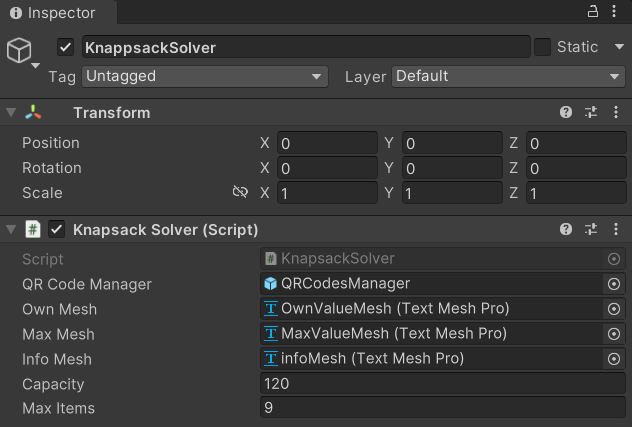
\includegraphics[scale=0.8]{images/knapsackEditor}
    \caption{KnapsackSolver Objekt im Editor}
    \label{fig:Knapsack_Editor}
\end{figure}

Anzumerken auf dieser Abbildung sind die Werte des \textit{KnapsackSolver} Skripts, die direkt im Unity Inspektor verändert
und übergeben werden können. Diese Werte und deren Beschreibung sind die folgenden:

\begin{itemize}
    \item \textbf{QRCodesManager:} Referenz auf das \textit{QRCodesManager} Game Objekt aus der Level-2 Szene.
    \item \textbf{Own Mesh:} Referenz auf das \textit{OwnValueMesh} aus dem \textit{infoObjekt} aus der Level 2 Szene.
    \item \textbf{Max Mesh:} Referenz auf das \textit{MaxValueMesh} aus dem \textit{infoObjekt} aus der Level 2 Szene.
    \item \textbf{Info Mesh:} Referenz auf das \textit{infoMesh} aus dem \textit{infoObjekt} aus der Level 2 Szene.
    \item \textbf{Capacity:} Integer Wert, der die Kapazität für den \textit{Knapsack Algorithmus} festlegt.
    \item \textbf{Max Items:} Repräsentiert die maximale Anzahl an Items die in das Inventar gelegt werden können. Dies
    dient als extra Bedingung für den \textit{Knapsack Algorithmus}.\\
\end{itemize}

\subsubsection{KnapsackSolver Klassenvariablen}
\begin{lstlisting}[style=csharp, caption={Klassenvariablen des KnapsackSolvers}, label=code:Klassenvariablen_kn]
public GameObject QRCodeManager;
public TextMeshPro ownMesh;
public TextMeshPro maxMesh;
public TextMeshPro infoMesh;

public int[,] usedItems;
public int capacity = 120;
public Dictionary<int, QRData> items;
public int maxItems = 9;

private int[,] inventory;
\end{lstlisting}\\
\\
Die im Codeabschnitt \ref{code:Klassenvariablen_kn} gezeigten Klassenvariablen gehören zur \textit{KnapsackSolver}-Klasse.
Diese Variablen werden verwendet, um Objekte und Werte innerhalb des Unity Editors zu repräsentieren, die entweder direkt
festgelegt und übergeben werden oder von anderen Klassen aus Funktionalitätsgründen benötigt werden. Die öffentlichen
(\textit{public}) Variablen ermöglichen einen direkten Zugriff auf diese Objekte in der eigenen oder einer anderen Klasse.

Das \textit{2D int Array inventory} spielt eine entscheidende Rolle im Verlauf des \textit{KnapsackSolvers}, da es verwendet
wird, um das individuell vom Benutzer zusammengestellte Inventar zu verarbeiten und zu berechnen.

Die privaten (\textit{private}) Klassenvariablen dienen hauptsächlich dem lokalen Speichern von Werten, die nur innerhalb
der \textit{KnapsackSolver}-Klasse benötigt werden und keinen Zugriff von außen erfordern.

\subsubsection{Start des KnapsackSolvers}
Die \textbf{Start()} Funktion, die in folgendem Codeabschnitt \ref{code:kn_start} abgebildet ist, ist der Startpunkt d
es \textit{KnapsackSolvers}.

\begin{lstlisting}[style=csharp, caption={Klassenvariablen der InventoryController Klasse}, label=code:kn_start]
void Start()
{
    items = new QRItem(0).items;
    EventManager.OnGridUpdate += SetInventory;
}
\end{lstlisting}\\
\\
Zu Beginn der Funktion wird dem Dictionary \textit{items} ein neues Objekt des Typs \textit{QRitem} zugewisen, wobei die
\textit{ID} 0 übergeben wird. Dies ermöglicht den Zugriff auf das Dictionary in der \textit{QRItem} Klasse welches alle
Daten der einzelnen Items enthält. Anschließend wird das Event \textit{OnGridUpdate} des \textit{EventManagers} ausgelöst
und die Funktion \textbf{SetInventory()} aufgerufen. Letztere ist eine Rückruffunktion, die als Reaktion auf das Ereignis
aufgerufen wird und die Aufgabe hat, das Inventar zu aktualisieren. Diese Funktion sieht wie folgt aus:
\begin{lstlisting}[style=csharp, caption={Inventar setzen}, label=code:kn_start]
public void SetInventory(int[,] newInventory)
{
    inventory = newInventory;
    CalculateKnapsack();
}
\end{lstlisting}
\\
Um stets mit dem aktuellen Inventar zu rechnen, wird bei jedem mal, bei dem die \textbf{SetInventory()} Funktion
aufgerufen wird, das aktuelle Inventar (\textit{inventory}) mit dem neuen Inventar in dem ein neues Item enthalten ist
(\textit{newInventory}) aktualisiert, um anschließend die tatsächlichen Werte zu berechnen, wird die \textbf{CalculateKnapsack()}
Funktion aufgerufen. Der Code zu dieser Funktion:
\begin{lstlisting}[style=csharp, caption={Berechnungsfunktion}, label=code:kn_calc]
void CalculateKnapsack()
{
    int maxValue = KnapsackMaxValue(out usedItems);
    int inventoryValue = -1;
    maxMesh.text = "Maximal erreichbarer Wert: " + maxValue.ToString();
    try
    {
        inventoryValue = KnapsackInventoryValue(inventory);
        if (maxValue == inventoryValue)
        {
            UpdateInfoMesh("Optimale Lösung gefunden", Color.green);
        }
        else
        {
            infoMesh.text = "";
        }
        ownMesh.text = "Erreichter Wert: " + inventoryValue.ToString();
    }
    catch (Exception e)
    {
        Debug.LogError("Error calculating inventory value: " + e.Message);
    }
}
\end{lstlisting}\\
\\
Diese Funktion stellt den Start des Knapsack-Algorithmus als auch der Berechnung des eigenen Inventars dar. Der berechnete
maximale erreichbare Wert, der von Funktion \textbf{KnapsackMaxValue} errechnet und zurückgegeben wird, wird der Variable
\textit{maxValue} zugewiesen für späteres vergleichen. Auch gibt diese Funktion das Array welches eine perfekte Lösung
repräsentiert zurück (\textit{out usedItems}).

Um dem Benutzer anzuzeigen, was der errechnte maximal erreichbare Wert ist, wird anschließend der Text des \textit{maxMash}
geändert, um diesen anzuzeigen. Bei der Berechnung des individuell zusammengestellten Inventars wird hier aus Sicherheitsgründen
ein \textit{try/catch} Block durchlaufen um potenzielle Fehler und einen dadurch verursachten Programmcrash zu vermeiden.
In diesem Block wird versucht, das eigene Inventar anhand des zusammengestellten Inventars (\textit{inventory}) zu berechnen.
Darauffolgend wird nun überprüft, ob der Benutzer mit seiner Lösung eine perfekte Lösung gefunden hat und in diesem Fall,
wird das \textit{infoMesh} anhand der \textbf{UpdateInfoMesh} Funktion mit einer dementsprechenden Erfolgsmeldung und Farbe
aktualisiert. Falls dies nicht der Fall ist, bleibt dieses einfach leer. Nach dieser Überpüfung der errechnete Wert des
Inventars in dem \textit{ownMesh} dargestellt, um dem Benutzer zu zeigen, was dieser erreicht hat.
\\
\\
Um den beschriebene Fall zu veranschaulichen, in dem der Benutzer eine perfekte Lösung gefunden hat, wird hierzu ein Beispiel
herangezogen.

\begin{quote}
Angenommen, der Benutzer stellt ein Inventar zusammen, welches den maximal möglichen Wert erreicht. Nach erneutem Berechnen
wird dem Benutzer wie in folgender Abbildung \ref{fig:foundperfsol} anschließend folgende Ansicht präsentiert:
\begin{figure}[H]
    \centering
    \includegraphics[scale=0.6]{images/foundperfsol}
    \caption{Eine perfekte Lösung gefunden}
    \label{fig:foundperfsol}
\end{figure}
TODO: Bild machen mit perfekten Lösung und in folgendem Text IDs einfügen\\
Auf dieser Abbildung ist zu sehen, dass das Inventar mit den Gegenständen mit folgenden \textit{IDs}: ., .,. ,. ,. befüllt
ist und der errechnete Wert dieses Inventars dem der perfekten Lösung gleicht. Diese Erkenntnis ist anhand des \textit{infoMesh}
zu erkennen, in dem eine Erfolgsnachricht in grüner Farbe dargestellt ist.
\end{quote}

\subsubsection{Knapsack-Algorithmus Implementierung}
Dieser Abschnitt behandelt die Implementierung der allgemeinen Variation des 0/1 Knapsack-Problems anhand des dynamischen
Algorithmus zur Lösung des Knapsack-Problems. Die Implementierung erfolgt in der Funktion \textbf{KnapsackMaxValue()}.
Diese Funktion gibt ein zweidimensionales Array zurück, das eine perfekte Lösung für das Problem speichert. Die Funktion
besteht im Wesentlichen aus zwei wichtigen Abschnitten:

Der erste Abschnitt beinhaltet die Implementierung des Algorithmus selbst, während der zweite Abschnitt dazu dient, die
ausgewählten Gegenstände zu verfolgen, die zur Erreichung des maximalen Werts verwendet wurden. Anhand dieser Gegenstände
wird dann das Array \textit{usedItems} erstellt, welches die perfekte Lösung repräsentiert.

Im Folgenden wird der Code dieser Funktion präsentiert:
\begin{lstlisting}[style=csharp, caption={Knapsack Algorithmus / Item Backtracking}, label=code:startKnapsack]
public int KnapsackMaxValue(out int[,] usedItems)
{
    int n = items.Count;
    int[,] dp = new int[n + 1, capacity + 1];
    bool[,] selected = new bool[n + 1, capacity + 1];
    for (int i = 0; i <= n; i++)
    {
        for (int w = 0; w <= capacity; w++)
        {
            if (i == 0 || w == 0)
                dp[i, w] = 0;
            else if (i <= maxItems && items[i].weight <= w)
            {
                int newValue = items[i].value + dp[i - 1, w - items[i].weight];
                if (newValue > dp[i - 1, w])
                {
                    dp[i, w] = newValue;
                    selected[i, w] = true;
                }
                else
                {
                    dp[i, w] = dp[i - 1, w];
                    selected[i, w] = false;
                }
            }
            else
            {
                dp[i, w] = dp[i - 1, w];
                selected[i, w] = false;
            }
        }
    }
    int[,] tempUsedItems = new int[3, 3];
    int row = n;
    int col = capacity;
    int rowIndex = 0;
    int colIndex = 0;
    while (row > 0 && col > 0 && rowIndex < 3 && colIndex < 3)
    {
        if (selected[row, col] && colIndex < maxItems)
        {
            tempUsedItems[rowIndex, colIndex] = items[row].id;
            col -= items[row].weight;
            row--;
            colIndex++;
            if (colIndex >= 3)
            {
                colIndex = 0;
                rowIndex++;
            }
        }
        else
        {
            row--;
        }
    }
    usedItems = tempUsedItems;
    return dp[n, capacity];
}
\end{lstlisting}
Die Implementierung des Knapsack-Algorithmus in den Zeilen drei bis 32 der Funktion \textbf{KnapsackMaxValue()} dieses
Abschnitts entspricht im Wesentlichen dem bereits erklärten Pseudocode. Ein wesentlicher Unterschied besteht jedoch darin,
dass diese spezielle Implementierung eine zusätzliche Bedingung berücksichtigt. Diese Bedingung besagt, dass zur Berechnung
des maximalen Werts und damit der optimalen Lösung maximal 9 Gegenstände in die Berechnung miteinbezogen werden können.
Dies ist darauf zurückzuführen, dass im vorliegenden Inventar-Objekt nur 9 verfügbare Zellen vorhanden sind, in die ein
Gegenstand eingefügt werden kann. Die Erfüllung dieser Bedingung wird in dem
\textit{else-if}-Zweig $i \leq \text{maxItems} \land \text{items}[i].\text{weight} \leq w$ gewährleistet.

Zusätzlich wird ein Array von booleschen Werten namens \textit{selected} erstellt, um im Verlauf der Berechnung diejenigen
Gegenstände zu markieren, die ausgewählt wurden (\textit{selected = true}). Dieses Array wird verwendet, um im zweiten
Teil der Funktion die perfekte Lösung zusammenzustellen.\\

\subsubsection*{Aufbau und Interpretation der selected Tabelle}
Angenommen, es sind die folgenden  5 Gegenstände (indiziert von 1 bis 5) mit den folgenden Werten und Gewichten gegeben:
\[
\begin{array}{|c|c|c|}
\hline
\text{Gegenstand} & \text{Wert} & \text{Gewicht} \\
\hline
1 & 10 & 5 \\
\hline
2 & 6 & 4 \\
\hline
3 & 8 & 3 \\
\hline
4 & 3 & 2 \\
\hline
5 & 7 & 1 \\
\hline
\end{array}
\]
\\
Und die \textit{Kapazität} des Rucksacks liegt bei 5. Aufgrund dieser Angaben wird die \textit{selected}-Matrix nach
Ausführung des Knapsack-Algorithmus basierend auf den ausgewählten Gegenständen gefüllt. Diese Matrix sieht dann folgendermaßen
aus:

\[
\begin{array}{|c|c|c|c|c|c|}
\hline
& 0 & 1 & 2 & 3 & 4 \\
\hline
0 & \text{false} & \text{false} & \text{false} & \text{false} & \text{false} \\
\hline
1 & \text{false} & \text{false} & \text{false} & \text{false} & \text{true} \\
\hline
2 & \text{false} & \text{false} & \text{false} & \text{true} & \text{true} \\
\hline
3 & \text{false} & \text{false} & \text{true} & \text{true} & \text{true} \\
\hline
4 & \text{false} & \text{true} & \text{true} & \text{true} & \text{true} \\
\hline
5 & \text{false} & \text{true} & \text{true} & \text{true} & \text{true} \\
\hline
\end{array}
\]
Für die Interpretation der \textit{selected}-Matrix ist es wichtig zu verstehen, wie sie funktioniert. Jede Zelle in dieser
Matrix gibt an, ob der entsprechende Gegenstand in der perfekten Lösung des Knapsack-Problems enthalten ist (\textit{true})
oder nicht (\textit{false}). Als Beispiel zeigt die Zelle $selected[4][3]$, dass der Gegenstand 4 in der perfekten Lösung
miteinbezogen wurde, als die Kapazität des Rucksacks 3 betrug. Diese Informationen ermöglichen folgende Schlussfolgerungen:
\begin{enumerate}
\item Der Index \textbf{i} in $selected[i][j]$ repräsentiert den Gegenstand, der in Betracht gezogen wird.
\item Der Index \textbf{j} in $selected[i][j]$ gibt die Kapazität des Rucksacks an, die für diese Teillösung verwendet
wurde.
\end{enumerate}

Der zweite Teil der Funktion, der sich um das \textit{Backtracking} der in der perfekten Lösung verwendeten Items kümmert,
beginnt damit, dass Variablen initialisiert werden, um den aktuellen Zeilen- und Spaltenindex in dem \textit{selected}
Array zu verfolgen, sowie \textit{Indezes} für das temporäre Array, die die ausgewählten Gegenstände speichert. Zunächst
wird eine Schleife gestartet, um durch das \textit{selected} Array
zu iterieren und die ausgewählten Gegenstände zu identifizieren.

Während der Iteration werden Bedingungen überprüft, um zu entscheiden, ob ein Gegenstand ausgewählt wurde. Wenn ein
Gegenstand ausgewählt wird, wird seine \textit{ID} in das temporäre Array (\textit{tempUsedItems})eingefügt, und die
Position in der Tabelle wird aktualisiert, indem das Gewicht des ausgewählten Gegenstands von der aktuellen Kapazität
subtrahiert wird. Die Schleife durchläuft die Tabelle und fährt fort, bis entweder die erste Zeile oder Spalte erreicht
wird oder die maximal zulässige Anzahl von ausgewählten Gegenständen erreicht ist.

Wenn ein Gegenstand ausgewählt wird, wird seine ID in die temporäre Matrix eingefügt, um die ausgewählten Gegenstände zu
speichern. Die Indizes der temporären Matrix werden aktualisiert, um den nächsten verfügbaren Speicherplatz zu zeigen.
Andernfalls wird der Zeilenindex dekrementiert, um zur vorherigen Zeile in des \textit{selected} Arrays zu gehen.

Am Ende der Funktion wird der Wert von \textit{usedItems} mit dem ermittelten Array \textit{tempUsedItems} überschrieben
und der maximale Wert des Rucksacks wird zurückgegeben.

\subsubsection{Berechnung des eigenen Inventars}
Die letzte Berechnung, die durchgeführt wird, ist die Berechnung des eigenen Inventars. Dies wird mittels der \textbf{KnapsackInventoryValue()}
Funktion erreicht. Der Code dieser Funktion:
\begin{lstlisting}[style=csharp, caption={Funktion um eigenes Inventar zu brechnen}]
public int KnapsackInventoryValue(int[,] inventory)
{
    if (inventory == null)
    {
        throw new System.Exception("Inventory is null");
    }
    int totalValue = 0;
    foreach (var item in items.Values)
    {
        int itemId = item.id;
        int itemValue = item.value;
        for (int j = 0; j < inventory.GetLength(0); j++)
        {
            for (int k = 0; k < inventory.GetLength(1); k++)
            {
                if (inventory[j, k] == itemId)
                {
                    totalValue += itemValue;
                }
            }
        }
    }
    return totalValue;
}
\end{lstlisting}
In dieser Funktion wird der Gesamtwert des aktuellen Inventars berechnet, welches durch das zweidimensionales Array
(\textit{inventory}) repräsentiert wird. Zunächst wird überprüft, ob das übergebene Inventar korrekt gesetzt wurde und
ob es \textit{null} ist oder nicht. Falls es \textit{null} ist, wird eine \textit{Exception} geworfen. Falls das Inventar
nicht leer ist, wird die Variable \textit{totalValue} initialisiert, um den Gesamtwert des Inventars zu speichern.
Anschließend wird eine \textit{foreach}-Schleife über jedes Element des Dictionaries \textit{items} durchgeführt, wobei
die \textit{ID} und der Wert \textit{value} jedes Elements ermittelt und in \textit{itemId} und \textit{itemValue}
gespeichert werden.

Anschließend werden zwei verschachtelte \textit{for}-Schleifen verwendet, um jedes Element im \textit{inventory}-Array
zu durchlaufen. Wenn die \textit{ID} des Gegenstands im \textit{inventory}-Array gefunden wird, wird der Wert dieses
Gegenstands zum Gesamtwert \textit{totalValue} addiert. Nach Abschluss der beiden \textit{for}-Schleifen wird dieser
ert schließlich zurückgegeben.

\subsubsection{InfoMesh aktualisieren}
Der \textit{KnapsackSolver} enthält zwei Funktionen, die sowohl in der Klasse selbst als auch in der
\textit{InventoryController} Klasse gebraucht werden. Die Funktion \textbf{SetInventory()} wurde bereits erklärt und
die zweite Funktion ist die folgende:

\begin{lstlisting}[style=csharp, caption={Funktion um InfoMesh zu verändern}]
public void UpdateInfoMesh(string input, Color color)
{
    infoMesh.color = color;
    infoMesh.text = input;
}
\end{lstlisting}
Diese Funktion ist wichtig für das Ändern der Fehlermeldungen, Erfolgsmeldungen als auch der Farbe des Textes in dem
\textit{infoMesh} und sie wird von dieser Klasse selbst auch im \textit{InventoryController} verwendet.

\subsection{Anzeigen der perfekten Lösung}\marginpar{\small\(\rightarrow\) SKREPEK}
Im zweiten Anwendungsszenario ist das Anzeigen der perfekten Lösung von entscheidender Bedeutung. Es ermöglicht dem Benutzer,
eine perfekte Lösung zu visualisieren, um zu verstehen, wie sie aussieht und welche Gegenstände sie enthält.

Für die Umsetzung dieser Funktion wird das \textit{bestSolutionPrefab} verwendet. Dieses Prefab erfüllt nicht nur die
Rolle eines allgemeinen Vorlagenobjekts für die perfekte Lösung, sondern dient auch als Träger einer wichtigen Komponente,
nämlich des \textit{PerfectSolutionVisualizer.cs} Skripts. Durch die Implementierung der \textbf{PerfectSolutionVisualizer}
Klasse bietet dieses Skript eine Vielzahl grundlegender Funktionen, die für die Darstellung der perfekten Lösung von
entscheidender Bedeutung sind.

Die Struktur und Hierarchie des Prefabs im Unity Editor sind entsprechend konzipiert, um eine effektive und übersichtliche
Verwaltung zu gewährleisten. Die visuelle Darstellung sowie die logische Organisation der enthaltenen Elemente sind darauf
ausgerichtet, dem Entwickler eine intuitive Handhabung und Anpassung zu ermöglichen.

Eine sorgfältige Gestaltung und Implementierung des \textit{bestSolutionPrefab} und des zugehörigen \textit{PerfectSolutionVisualizer.cs}
Skripts sind entscheidend, um dem Benutzer ein nahtloses und aussagekräftiges Erlebnis zu bieten. Durch die präzise
Visualisierung und die transparente Darstellung der perfekten Lösung kann der Benutzer nicht nur die Optimierungsmöglichkeiten
des Knapsack-Problems besser verstehen, sondern auch wichtige Einblicke in die Funktionsweise des Algorithmus gewinnen.
Das Prefab welches dies erreicht, ist in folgender Abbildung \ref{fig:InvPref} zu sehen:
\begin{figure}[H]
\centering
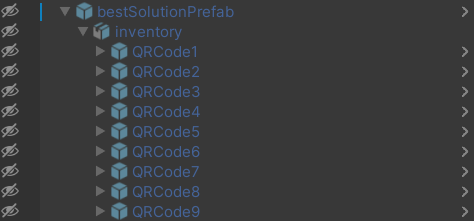
\includegraphics[scale=1]{images/bestSolPref}
\caption{Prefab Hirarchie und Aufbau im Unity Editor}
\label{fig:InvPref}
\end{figure}

Auf dieser Abbildung ist sowohl die Hierarchie als auch der allgemeine Aufbau des Prefabs zu sehen. Die Hierarchie dieses
Prefabs zeigt, dass es aus dem Inventar-Objekt besteht, unter dem mehrere einzelne \textit{QRCode} Prefabs angeordnet sind.
Besonders wichtig ist die Anordnung der \textit{QRCode} Prefabs. In jeder einzelnen Zelle des Inventar-Objekts befindet
sich jeweils ein Prefab, wie in der Abbildung dargestellt. Dies dient dazu, anhand der errechneten und gespeicherten
perfekten Lösung das Prefab und die darin enthaltenen QRCode-Prefabs wie ein Array durchlaufen zu können. Mithilfe der
eindeutigen ID jedes QRCode-Prefabs kann dann das darin gespeicherte Modell aktiviert werden. Dies stellt die Grundlage
für das Anzeigen einer perfekten Lösung dar.
\\
\\
Das dem Prefab angehängte Script benötigt Zugriff auf mehrere verschiedene Objekte, um erfolgreich zu funktionieren. In
folgender Abbildung \ref{code:bestSol_Editor} ist das Game Objekt selbst in Unity zu sehen.

\begin{figure}[H]
\centering
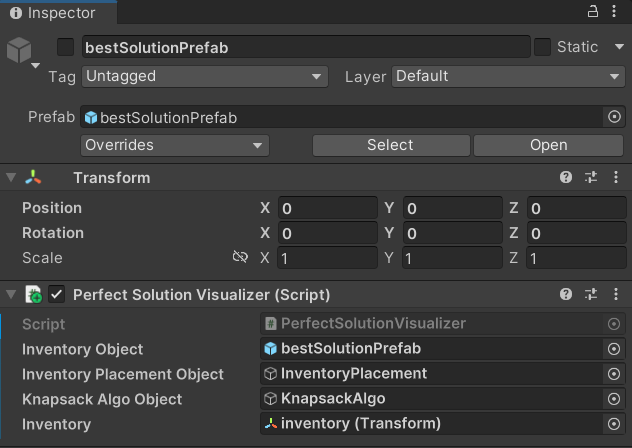
\includegraphics[scale=0.8]{images/bestSolPref_Editor}
\caption{Game Objekt im Unity Editor}
\label{fig:bestSol_Editor}
\end{figure}

Auf dieser Abbilding ist das \textit{bestSolutionPrefab} Game Objekt mit den zugehörigen Komponenten in Unity selbst zu
sehen. An der Komponente welches das Skript repräsentiert ist zu sehen, dass dieses vier zu übergebende Objekte benötigt.
Darunter sind die folgenden:
\begin{itemize}
    \item \textbf{Inventory Object:} Eine Referenz auf das \textit{Prefab} für die perfekte Lösung.
    \item \textbf{Inventory Placement Object:} Eine Referenz auf das \textit{inventoryPlacement} Game Objekt.
    \item \textbf{Knapsack Algo Object:} Eine Referenz auf das \textit{KnapsackSolver} Game Objekt.
    \item \textbf{Inventory:} Eine Referenz auf das \textit{Inventory} Modell, das im Best Solution Prefab enthalten ist.
\end{itemize}

\subsubsection{Auslöser des Skripts}
Der Skript-Prozess zur Anzeige der perfekten Lösung wird durch einen simplen Knopfdruck ausgelöst. Der Knopf befindet
sich innerhalb des \textit{infoObject}, welches als Container für verschiedene Informationen oder Steuerelemente betrachtet
werden kann.

Wenn der Benutzer auf diesen Knopf klickt, startet das Skript zur Darstellung der perfekten Lösung. Es führt die notwendigen
Funktionen und Abläufe aus, um die perfekte Lösung zu visualisieren.

Abbildung \ref{fig:ScrAuf} zeigt den Aufruf des Skripts und verdeutlicht den Zusammenhang zwischen dem Knopf im \textit{infoObject}
und dem Start des Skripts. Durch diese klare Verbindung können Benutzer die perfekte Lösung leichter abrufen und verstehen,
was den gesamten Prozess zugänglicher macht.

\begin{figure}[H]
\centering
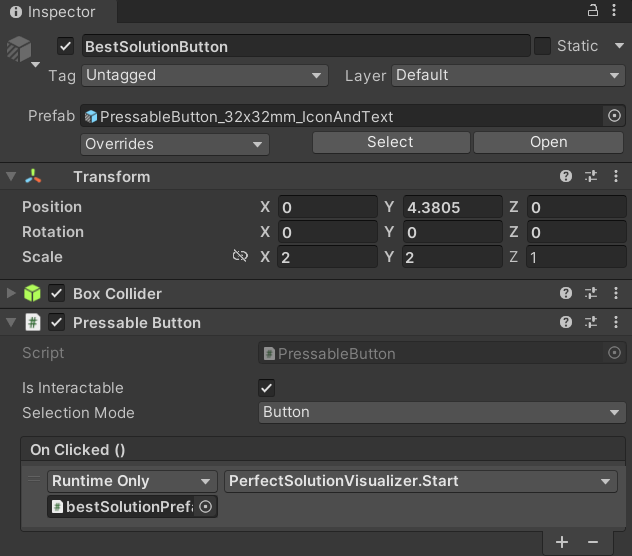
\includegraphics[scale=0.8]{images/perfSolBut}
\caption{Script Aufruf bei Knopfdruck}
\label{fig:ScrAuf}
\end{figure}

Auf dieser Abbildung ist zusätzlich noch anzumerken, dass das interaktive drücken eines Knopfes durch das bereitgestellte
Skript \textit{PressableButton} möglich gemacht wird. Dieses Skript stellt die Funktion \textbf{OnClicked()} bereit, welche
einen simplen Knopfdruck implementiert. Diese Funktion löst bei Knopfdruck anschließend die \textbf{Start()} Funktion des
\textit{bestSolutionVisualizer} aus.

\subsubsection{PerfectSolutionVisualizer Klassenvariablen}
\begin{lstlisting}[style=csharp, caption={Klassenvariablen des PerfectSolutionVisualizer}, label=code:Klassenvariablen_PSV]
public GameObject inventoryObject;
public GameObject inventoryPlacementObject;
public GameObject KnapsackAlgoObject;
public Transform inventory;

private PlaceObjectOnLookedAtDesk anchorScript;
private KnapsackScript knapsackScript;
private Vector3 originalInventoryPosition;
private int[,] perfectSolution;
private bool isClicked = false;
private int numRows = 3;
private int numColumns = 3;
\end{lstlisting}\\
Die im Codeabschnitt \ref{code:Klassenvariablen_PSV} gezeigten Klassenvariablen gehören zur \textit{PerfectSolutionVisualizer}
Klasse. Diese Variablen dienen dazu, Objekte und Werte innerhalb des Unity Editors zu repräsentieren, die entweder direkt
festgelegt und übergeben werden oder von anderen Klassen aus Funktionalitätsgründen benötigt werden. Durch die Verwendung
von öffentlichen (\textit{public}) Variablen ist ein direkter Zugriff auf diese Objekte in der eigenen oder einer anderen
Klasse möglich.

Besonders wichtig ist der Zugriff auf die Variablen \textit{inventoryPlacementObject} und \textit{KnapsackAlgoObject}, um
im weiteren Verlauf dieses Skripts auf die beiden angehängten Skripte dieser Game Objekte zuzugreifen. Diese Skripte
speichern die Position des Inventars und das \textit{usedItems}-Array. Die Position des originalen Inventars ist notwendig,
um die perfekte Lösung korrekt zu platzieren, während das \textit{usedItems}-Array später benötigt wird, um das
\textit{bestSolutionPrefab} anhand der gespeicherten Werte zu befüllen.

\subsubsection{Start des PerfectSolutionVisualizer}
Nachdem der Benutzer den \textit{BestSolutionButton} betätigt hat, wird der entscheidende Prozess zur Anzeige der perfekten
Lösung eingeleitet. Dieser Vorgang wird durch die Ausführung der \textbf{Start()} Funktion gestartet, wie im folgenden
Codeabschnitt \ref{code:Start_PSV} ersichtlich ist.
\begin{lstlisting}[style=csharp, caption={PerfectSolutionVisualizer Start}, label=code:Start_PSV]
public void Start()
{
    isClicked = !isClicked;
    if (isClicked == true)
    {
        anchorScript = inventoryPlacementObject.GetComponent<InventoryPlacementController>();
        originalInventoryPosition = anchorScript.objectPosition;
        knapsackSolver = KnapsackAlgoObject.GetComponent<KnapsackSolver>();
        perfectSolution = knapsackSolver.usedItems;
        printItems();
        setNewPosition();
        inventoryObject.SetActive(true);
        fillInventory();
    }
    else
    {
        inventoryObject.SetActive(false);
    }
}
\end{lstlisting}\\
Diese Funktion fungiert nicht nur als Initiator für das Anzeigen der perfekten Lösung, sondern auch für das Ausblenden
derselben. Eine zentrale Aufgabe besteht darin sicherzustellen, dass der Benutzer die Lösung nach Bedarf ein- oder
ausblenden kann. Zu diesem Zweck wird bei jedem Aufruf der Funktion die boolsche Variable \textit{isClicked} invertiert,
welche den Zustand des Buttons repräsentiert.

Basierend auf diesem boolschen Wert wird im weiteren Verlauf der Funktion entschieden, ob die perfekte Lösung sichtbar
gemacht werden soll oder nicht (\textit{inventoryObject.SetActive(true/false)}). Bei Bedarf werden die Positionsinformationen
des Objekts durch die \textit{objectPosition}-Variable der Klasse \textit{InventoryPlacementController} sowie das
\textit{usedItems}-Array der Klasse \textit{KnapsackSolver} gesichert. Anschließend werden die Funktionen \textbf{setNewPosition()}
und \textbf{fillInventory()} aufgerufen, um eine präzise Positionierung der perfekten Lösung zu gewährleisten und das
Inventar entsprechend mit den relevanten Objekten zu füllen.


\subsubsection{Perfekte Lösung platzieren}
Die Platzierung der perfekten Lösung ist wichtig, um zu garantieren, dass es für den Benutzer leicht und angenehm ist,
diese zu sehen.

Um dies zu garantieren, wird auf die Original-Position des Inventar-Objekts
(\textit{originalInventoryPosition}) zugegriffen und aufgrund dessen eine neue Position errechnet. Diese neue Position ist
um 0,5 Einheiten entlang der z-Achse und um 0.205 Einheiten entlang der y-Achse verschoben, damit dieses vor dem originalen
Inventar-Objekt platziert wird. Um es dem Benutzer jedoch angenehmer zu machen, die perfekte Lösung besser zu sehen, wird
abschließend die Rotation dieses Objekts noch geändert, um es um -45 Grad entlang der x-Achse zu kippen.
\begin{lstlisting}[style=csharp, caption={Neue Position setzen}, label=code:newPos_PSV]
private void setNewPosition()
{
    Vector3 newPosition = originalInventoryPosition + Vector3.forward * 0.5f + Vector3.up * 0.205f;
    inventoryObject.transform.position = newPosition;
    Quaternion objectRotation = Quaternion.Euler(-45f, 0f, 0f);
    inventoryObject.transform.rotation = objectRotation;
}
\end{lstlisting}\\

\subsubsection{Prefab füllen}
Aufgrund der Beschaffenheit des zuvor platzierten Objekts, das lediglich ein leeres Inventar-Objekt darstellt, ist es
notwendig, dieses im nächsten Schritt mit den passenden Elementen zu füllen oder die geeigneten Modelle zu aktivieren,
welche die perfekte Lösung repräsentieren. Diese Aufgabe wird durch den Aufruf der \textbf{fillInventory()} Funktion im
weiteren Verlauf des Skripts realisiert.
\begin{lstlisting}[style=csharp, caption={Inventar füllen}, label=code:invFül_PSV]
private void fillInventory()
{
    for (int i = 0; i < numRows; i++)
    {
        for (int j = 0; j < numColumns; j++)
        {
            int id = perfectSolution[i, j];
            if (perfectSolution[i, j] == 0)
                continue;
            else
            {
                string qrCodeName = "QRCode" + (i * numColumns + j + 1);
                Transform qrCodeTransform = inventory.Find(qrCodeName);
                if (qrCodeTransform != null)
                {
                    Transform childTransform = qrCodeTransform.Find(id.ToString());
                    if (childTransform != null)
                    {
                        childTransform.gameObject.SetActive(true);
                    }
                }
                else
                {
                    Debug.LogError($"QRCode {qrCodeName} not found in the inventory");
                }
            }
        }
    }
}
\end{lstlisting}\\
Die vorliegende Funktion durchläuft das zweidimensionale Array \textit{perfectSolution}, das die perfekte Lösung repräsentiert.
Zu Beginn wird die ID an der Stelle $[i, j]$ des Arrays gespeichert. An jeder Position wird zunächst überprüft, ob die
gespeicherte ID gleich 0 ist. In diesem Fall wird der Schleifendurchlauf mit \textit{continue} übersprungen, da der Wert
0 darauf hinweist, dass an dieser Stelle kein Item liegt.

Wenn der Wert an der Stelle $[i, j]$ größer als 0 ist, deutet dies darauf hin, dass an dieser Position im Inventar ein
konkretes Element vorliegt. Zur Identifizierung dieses Elements und zum Auffinden des entsprechenden QRItems wird ein
stringbasierter Bezeichner \textit{qrCodeName} generiert. Dieser Bezeichner wird durch die Konkatenation des Präfixes
\textit{QRCode} mit dem Ergebnis der Berechnung $i \times \text{numColumns} + j + 1$ erzeugt. Diese Berechnung berücksichtigt
die aktuelle Position im zweidimensionalen Array und ermöglicht die Erstellung eines eindeutigen Bezeichners für das QRItem.
Auf diese Weise wird das QRItem erfolgreich identifiziert und kann anschließend im Inventar lokalisiert werden.\\
\\
Um diesen Vorgang der Identifikation des korrekten \textit{QRItem} Prefabs besser zu veranschaulichen wird hierfür ein
Beispiel herangezogen, dass die Berechcnung anhand von Testwerten durchführt.

\begin{quote}
Angenommen in der Schleife hat \textbf{i} den Wert 1 und \textbf{j} den Wert 1. Dies bedeutet, dass das Array momentan
an der Stelle $[1, 1]$ steht. Das \texttt{bestSolutionPrefab} ist so strukturiert, dass der Index nicht mit 0, sondern
mit 1 beginnt. Daher wird in der Berechnung am Ende $+ 1$ hinzugefügt, um dies zu berücksichtigen. Somit wird an der
Stelle $[i, j]$ das \textit{QRItem5} dem Array zugeordnet.
\end{quote}

Nachdem das richtige \textit{QRItem} identifiziert wurde, wird anschließend das dem Inventar-Objekt untergeordnete
\textit{QRItem} Prefab mit diesem Namen gespeichert. Wenn dieses Objekt ungleich null ist, wird von diesem Prefab das
untergeordnete Modell anhand der zuvor gespeicherten \textit{ID} aktiviert, um es in dem Inventar-Raster anzuzeigen.
Andernfalls wird eine Fehlermeldung in die \textit{Logdatei} geschrieben. Der Zustand nach dem Abschluss dieser Funktion
ist in der folgenden Abbildung \ref{fig:perfSolUserPOV} zu sehen.
\begin{figure}[H]
    \centering
    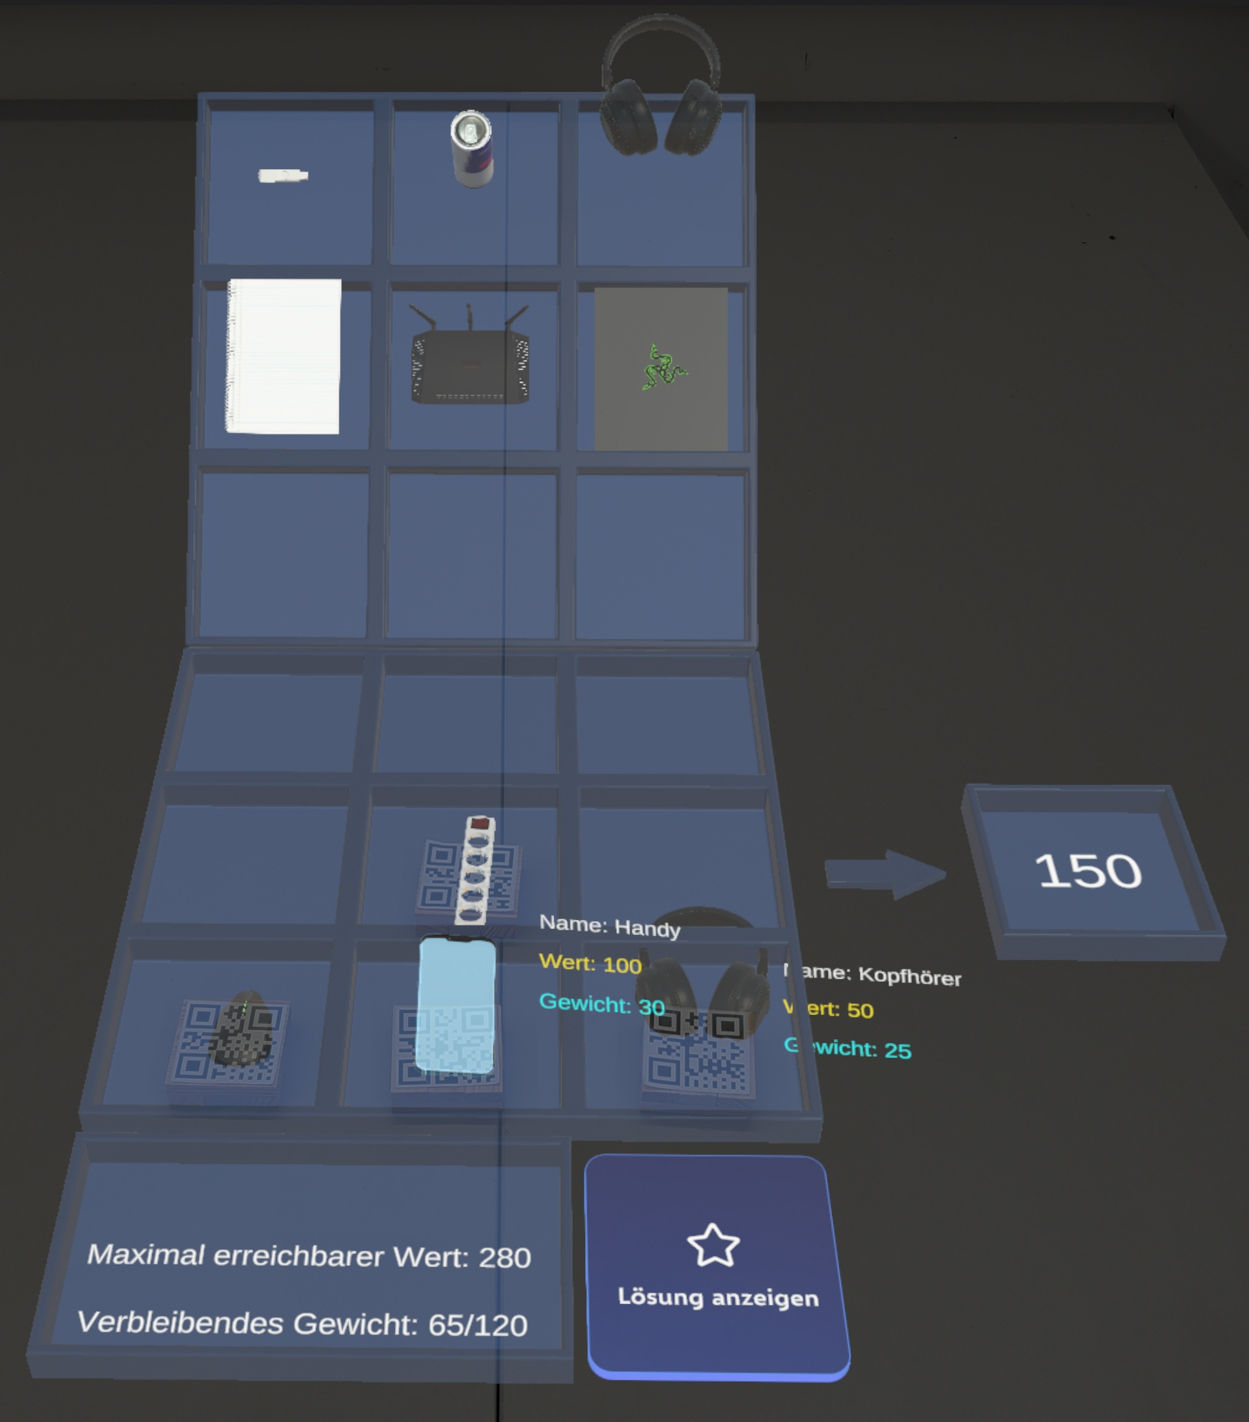
\includegraphics[scale=0.8]{images/perfSolUserPOV}
    \caption{Perfekte Lösung}
    \label{fig:perfSolUserPOV}
\end{figure}

\section{Performance und Qualtitätssicherung} \marginpar{\small\(\rightarrow\) HAYLAZ}
\subsection{Unit-Tests}
Unit-Tests sind ein entscheidender Bestandteil der Qualitätssicherung. Sie ermöglichen die Überprüfung der korrekten
Funktionalität einzelner Komponenten und stellen sicher, dass sie wie erwartet arbeiten. Im Rahmen dieses Projekts wurden
Unit-Tests verwendet, um den Knapsack-Algorithmus zu überprüfen. Die Tests wurden mithilfe des Unity Test Frameworks
erstellt und ausgeführt. Dieses Tool wurde speziell für die Erstellung und Ausführung von Unit-Tests in Unity entwickelt.
Durch die sorgfältige Gestaltung der Tests wurde sichergestellt, dass der Algorithmus nicht nur die erwarteten Ergebnisse
zurückgibt, sondern auch die vorgegebene Laufzeit einhält. Die Tests wurden innerhalb der Entwicklungsumgebung von Unity
durchgeführt, und die Ergebnisse wurden genau überwacht, um sicherzustellen, dass der Algorithmus zuverlässig funktioniert.

\subsection{Unity Test Framework}
Das Unity Test Framework bietet eine breite Palette von Funktionen, mit denen Entwickler umfassende Tests für ihre
Unity-Skripte schreiben und ausführen können. Dabei können verschiedene Aspekte der Skripte auf ihre korrekte Funktionalität
überprüft werden, darunter das Testen von Variablen, das Aufrufen von Funktionen und das Überprüfen von erwarteten Ergebnissen.
Dank dieser umfangreichen Funktionen können Entwickler sicherstellen, dass ihre Unity-Anwendungen robust und zuverlässig sind,
was eine solide Grundlage für die Qualitätssicherung schafft.

\subsection{Performance-Messung}
Die Performance des Knapsack-Algorithmus wurde mithilfe von Unit-Tests überprüft. Dabei wurde die Laufzeit des Algorithmus
für verschiedene Eingabegrößen gemessen. Die Ergebnisse wurden sorgfältig analysiert, um sicherzustellen, dass der Algorithmus
die erwartete Laufzeit einhält. Es wurden verschiedene Algorithmen und Implementierungen getestet, um die optimale Leistung
zu erzielen. Die Ergebnisse der Performance-Messung wurden genau überwacht, um sicherzustellen, dass der Algorithmus
zuverlässig und effizient arbeitet.

\begin{lstlisting}[style=csharp, caption={Unit Test Klasse}, label=code:UnitTest]
public class AlgoTest
{
GameObject testObject;
KnapsackScript knapsackScript;
int[,] usedItems;
int capacity = 120;
...
\end{lstlisting}\\

Dies ist eine Testklasse in C#, welche den Knapsack-Algorithmus implementiert und testet.

Dies ist eine Testklasse in C#, welche den Knapsack-Algorithmus implementiert und testet. Die Klasse AlgoTest enthält
Testfunktionen für zwei verschiedene Knapsack-Algorithmen. Es werden mehrere Variablen definiert, darunter ein testObject,
das zu testende knapsackScript und capacity, die maximale Größe des Rucksacks, die für die Tests benötigt wird. Die Methoden
SetUp und TearDown sind mit den Attributen [SetUp] und [TearDown] versehen. Diese Attribute werden vom Framework erkannt
und dienen dazu, nach jedem Test die Umgebung zu reinigen und neu aufzusetzen. Es wird eine Instanz des KnapsackScript
erstellt und wieder zerstört, um sicherzustellen, dass die Tests in einer sauberen Umgebung ausgeführt werden.

\begin{lstlisting}[style=csharp, caption={Unit Test Methode}, label=code:Test Methode]
// Ein Test verhält sich wie eine normale Methode
[Test]
public void KnapsackMaxValue_ReturnsCorrectValue()
{
// Gibt eine Menge von Gegenständen für den Rucksack an
Dictionary<int, QRData> items = new Dictionary<int, QRData>() {
{1, new QRData { id = 1, weight = 50, value = 100 }},
... //weitere Testobjekte

System.Random random = new System.Random();
for (int i = 11; i <= 100; i++)
{
int randomWeight = random.Next(1, 51);
int randomValue = random.Next(1, 101);

items.Add(i, new QRData { id = i, weight = randomWeight, value = randomValue });
}
\end{lstlisting}\\

Der Unit-Test \texttt{KnapsackMaxValue-ReturnsCorrectValue} testet die Methode \texttt{KnapsackMaxValue} des
\texttt{KnapsackScript}. Es werden verschiedene Gegenstände in dem Dictionary definiert. Außerdem werden noch weitere
Items mit zufälligen Werten in das Dictionary hinzugefügt, damit auch getestet wird, ob der Algorithmus konsistent richtige
Lösungen liefert.

\begin{lstlisting}[style=csharp, caption={Zeitmessung}, label=code:Zeitmessung]
// Messung der Ausführungszeit für KnapsackMaxValue
System.Diagnostics.Stopwatch knapsackMaxValueStopwatch = System.Diagnostics.Stopwatch.StartNew();
int maxValue = knapsackScript.KnapsackMaxValue(out usedItems);
knapsackMaxValueStopwatch.Stop();
Debug.Log($"Die Ausführungszeit von KnapsackMaxValue beträgt: {knapsackMaxValueStopwatch.ElapsedMilliseconds} ms");

// Messung der Ausführungszeit für KnapsackMaxValueRecursive
System.Diagnostics.Stopwatch recursiveStopwatch = System.Diagnostics.Stopwatch.StartNew();
int maxValueComp = KnapsackMaxValueRecursive(items.Count, capacity, items, new Dictionary<(int, int), int>());
recursiveStopwatch.Stop();
Debug.Log($"Die Ausführungszeit von KnapsackMaxValueRecursive beträgt: {recursiveStopwatch.ElapsedMilliseconds} ms");

// Überprüfen, ob die Werte übereinstimmen
Assert.AreEqual(maxValueComp, maxValue);
\end{lstlisting}\\

Anschließend wird die Ausführungszeit sowohl der iterativen (\texttt{KnapsackMaxValue}) als auch der
rekursiven (\texttt{KnapsackMaxValueRecursive}) Implementierung des Knapsack-Algorithmus gemessen. Schließlich wird
überprüft, ob beide Implementierungen denselben Wert zurückgeben.

\newpage

\begin{lstlisting}[style=csharp, caption={Rekursiver Algorithmus}, label=code:Rekursiver Algorithmus]
// Rekursive Implementierung des Knapsack-Algorithmus zur Berechnung des maximalen Werts
public int KnapsackMaxValueRecursive(int n, int remainingCapacity, Dictionary<int, QRData> items, Dictionary<(int, int), int> memo)
{
if (n == 0 || remainingCapacity == 0)
return 0;

if (memo.TryGetValue((n, remainingCapacity), out int memoizedValue))
return memoizedValue;

if (items[n].weight > remainingCapacity)
{
memo[(n, remainingCapacity)] = KnapsackMaxValueRecursive(n - 1, remainingCapacity, items, memo);
return memo[(n, remainingCapacity)];
}

int includedValue = items[n].value + KnapsackMaxValueRecursive(n - 1, remainingCapacity - items[n].weight, items, memo);
int excludedValue = KnapsackMaxValueRecursive(n - 1, remainingCapacity, items, memo);

int result = Math.Max(includedValue, excludedValue);

memo[(n, remainingCapacity)] = result;

return result;
}
\end{lstlisting}\\

Die Methode \texttt{KnapsackMaxValueRecursive} ist eine rekursive Implementierung des Knapsack-Algorithmus. Der maximale
Wert, den der Rucksack aufnehmen kann, wird berechnet, indem die Elemente rekursiv entweder eingeschlossen oder ausgeschlossen
werden.\\
Es wurde darauf geachtet, verschiedene Implementierungen zu testen, um sicherzustellen, dass die optimale
Implementierung verwendet wird.
\\
TODO: neue dynamische implementierung erwähnen und erklären
TODO: Grafik der Testergebnisse und Unterschiede der Laufzeiten von rekursiver und iterativer Implementierung erklären
\\
Dabei wird die rekursive Implementierung \texttt{KnapsackMaxValueRecursive} als Vergleich verwendet, um sicherzustellen, dass
auch die iterative Implementierung \texttt{KnapsackMaxValue} korrekt ist.
\chapter{Zusammenfassung und Abschluss}

\section{Ergebnis}
Hier steht der allgemeine Text für das Ergebnis

\section{Abnahme}
Hier steht der allgemeine Text für das Abnahme

\section{Zukunft}
Hier steht der allgemeine Text für die Zukunft
%\chapter{Drucken der Diplomarbeit}
\label{chap:Drucken}




\section{PDF-Workflow}
\label{sec:pdf}

In der aktuellen Version wird \latex\ so benutzt, dass damit direkt PDF-Dokumente (ohne den früher üblichen Umweg über DVI und PS) erzeugt werden.
%Zur Arbeit mit dem Sumatra PDF-Viewer unter Windows sind entsprechende Ausgabeprofile für TexNicCenter vorbereitet, die aus der Datei \verb!_tc_output_profiles_sumatra.tco! importiert werden können (siehe dazu die Information in Anhang \ref{sec:EinstellungAusgabeprofile}).


\section{Drucken}

\subsection{Drucker und Papier}

Die Diplomarbeit sollte in der Endfassung unbedingt auf einem
qualitativ hochwertigen Laserdrucker ausgedruckt werden, Ausdrucke
mit Tintenstrahldruckern sind \emph{nicht} ausreichend. Auch das
verwendete Papier sollte von guter Qualität (holzfrei) und
üblicher Stärke (mind.\ $80\; {\mathrm g} / {\mathrm m}^2$) sein.
Falls \emph{farbige} Seiten notwendig sind, sollte man diese einzeln%
\footnote{Tip: Mit \emph{Adobe Acrobat} lassen sich sehr einfach einzelne Seiten
des Dokuments für den Farbdruck auswählen und zusammenstellen.}
auf einem Farb-Laserdrucker ausdrucken und dem Dokument beifügen.

Übrigens sollten \emph{alle} abzugebenden Exemplare {\bf
gedruckt} (und nicht kopiert) werden! Die Kosten für den Druck
sind heute nicht höher als die für Kopien, der
Qualitätsunterschied ist jedoch -- \va\ bei Bildern und Grafiken
-- meist deutlich.


\subsection{Druckgröße}

Ein häufiger und leicht zu übersehender Fehler beim Ausdrucken von
PDF-Dokumenten wird durch die versehentliche Einstellung der
Option "`Fit to page"' im Druckmenü verursacht, wobei die Seiten
meist zu klein ausgedruckt werden. überprüfen Sie daher die Größe
des Ausdrucks anhand der eingestellten Zeilenlänge oder mithilfe
einer Messgrafik, wie am Ende dieses Dokuments gezeigt.
Sicherheitshalber sollte man diese Messgrafik bis zur
Fertigstellung der Arbeit beizubehalten und die entsprechende
Seite erst ganz am Schluss zu entfernen.
Wenn, wie häufig der Fall, einzelne Seiten getrennt in Farbe gedruckt 
werden, so sollten natürlich auch diese genau auf die Einhaltung der Druckgröße 
kontrolliert werden!




\section{Binden}

Die Endfassung der Diplomarbeit ist in fest gebundener Form einzureichen.%
Dabei ist eine Bindung zu verwenden, die das Ausfallen von einzelnen Seiten
nachhaltig verhindert, \zB durch eine traditionelle Rückenbindung
(Buchbinder) oder durch handelsübliche Klammerungen aus Kunststoff
oder Metall. Eine einfache Leimbindung ohne Verstärkung ist
jedenfalls \emph{nicht} ausreichend.


Falls man -- was sehr zu empfehlen ist -- die Arbeit bei einem
professionellen Buchbinder durchführen lässt, sollte man auch auf
die Prägung am Buchrücken achten, die kaum zusätzliche Kosten
verursacht. Üblich ist dabei die Angabe des Familiennamens des
Autors und des Titels der Arbeit. Ist der Titel der Arbeit zu
lang, muss man notfalls eine gekürzte  Version angeben, wie \zB:
%
\begin{center}
\setlength{\fboxsep}{3mm}
\fbox{
\textsc{Schlaumeier}
\textperiodcentered\ \textsc{Parz.\ Lösungen zur allg.\ Problematik}}
\end{center}
%



\section{Elektronische Datenträger (CD-R, DVD)}
Speziell bei Arbeiten im Bereich der Informationstechnik (aber
nicht nur dort) fallen fast immer Informationen an, wie Programme,
Daten, Grafiken, Kopien von Internetseiten \usw, die für eine
spätere Verwendung elektronisch verfügbar sein sollten.
Vernünftigerweise wird man diese Daten während der Arbeit bereits
gezielt sammeln und der fertigen Arbeit auf einer CD-ROM oder DVD
beilegen. Es ist außerdem sinnvoll -- schon allein aus Gründen der
elektronischen Archivierbarkeit -- die eigene Arbeit selbst als
PDF-Datei beizulegen.%
\footnote{Auch Bilder und Grafiken könnten in elektronischer Form nützlich
sein, die \latex- oder Word-Dateien sind hingegen überflüssig.}


Falls ein elektronischer Datenträger (CD-ROM oder DVD) beigelegt
wird, sollte man auf folgende Dinge achten:
%
\begin{enumerate}
\item Jedem abzugebenden Exemplar muss eine identische Kopie des
Datenträgers beiliegen. %
\item Verwenden Sie qualitativ hochwertige Rohlinge und überprüfen
Sie nach der Fertigstellung die tatsächlich gespeicherten Inhalte
des Datenträgers! %
\item Der Datenträger sollte in eine im hinteren Umschlag
eingeklebte Hülle eingefügt sein und sollte so zu entnehmen sein,
dass die Hülle dabei \emph{nicht} zerstört wird (die
meisten Buchbinder haben geeignete Hüllen parat). %
\item Der Datenträger muss so beschriftet sein, dass er der
Diplomarbeit eindeutig zuzuordnen ist, am Besten durch ein
gedrucktes Label oder sonst durch \emph{saubere}
Beschriftung mit der Hand und einem feinen, wasserfesten Stift. %
\item Nützlich ist auch ein (grobes) Verzeichnis der Inhalte des
Datenträgers (wie exemplarisch in Anhang \ref{app:cdrom}).
\end{enumerate}

%\chapter[Hinweise für \emph{Word}-Benutzer]{Hinweise für \emph{Word}-Benutzer%
\protect\footnote{Dieses Kapitel ist ein Relikt aus früheren Versionen, die%
umfangreiche Hinweise für die Erstellung von Diplomarbeiten mit \emph{Word} enthielten.}% 
}
\label{chap:Word}

Wie bereits in der Einleitung erwähnt, ist \emph{Word} für das
Schreiben von umfangreicheren Werken wie Bücher und
Diplomschriften nur bedingt geeignet. \emph{Word} besitzt zwar
einen immens großen Funktionsumfang,  manche einfach anmutende
Aufgaben erfordern aber bisweilen sehr umständliche Maßnahmen oder
sind schlichtweg unmöglich. Eine unangenehme Eigenschaft ist
weiters, dass Word-Dokumente gelegentlich in fehlerhafte Zustände
geraten können, die man nur mehr durch Rückkehr zu einer vorher
gesicherten Version (sofern vorhanden) reparieren kann. 
Tatsächlich scheinen sich bei den neueren
(XML-basierten) Office-Versionen einige der bisherigen
Schwierigkeiten noch verstärkt zu haben, \zB\ die noch
umständlichere (und empfindliche) Verwaltung von Formatvorlagen.

Das soll nicht heißen, dass mit entsprechender Disziplin und Detailkenntnis
nicht auch mit \emph{Word} große Dokumente sauber und erfolgreich hergestellt
werden können, wie auch die Produkte mancher Sachbuchverlage zeigen. Ich persönlich würde aber dazu nicht ermutigen und habe daher die in diesem Kapitel früher zusammengefassten Hinweise für den Umgang mit \emph{Word} entfernt.


Falls man \emph{Word} ohnehin
nur oberflächlich beherrscht, sollte man daher überlegen, ob man es
nicht gleich mit \latex versuchen möchte. 
Bei durchaus vergleichbarem Lernaufwand wird sich wahrscheinlich
das Ausmaß an Frustration -- mit Sicherheit aber das Ergebnis -- 
deutlich unterscheiden.
Falls man von Word 
auf \latex umzusteigen möchte und zu diesem Zeitpunkt bereits
umfangreiches Material in \emph{Word} vorhanden ist, sollte man sich das
Programm \texttt{rtf2latex}%
\footnote{\zB \url{www.tex.ac.uk/tex-archive/support/rtf2latex2e/}}
ansehen, das \emph{Rich Text Format} (RTF) in \latex-Dateien übersetzt.


Als professionelle WYSIWYG-Alternative bietet sich \zB\ \emph{Indesign} von \emph{Adobe} an, das für den Schriftsatz angeblich ähnliche Algorithmen wie \latex\ verwendet. Bezüglich mathematischer Elemente, gleitender Platzierung von Abbildungen und Tabellen, sowie der Verwaltung von Literaturangaben kommt Indesign allerdings an \latex\ derzeit nicht heran.

%\chapter{Schlussbemerkungen}
\label{cha:Schluss}

An dieser Stelle sollte eine Zusammenfassung der Diplomarbeit
stehen, in der auch auf den Entstehungsprozess, persönliche
Erfahrungen, Probleme bei der Durchführung,
Verbesserungsmöglichkeiten, mögliche %
Erweiterungen \usw\ eingegangen werden kann. War das Thema richtig
gewählt, was wurde konkret erreicht, welche Punkte blieben offen
und wie könnte man von hier aus weiter arbeiten?


\section{Lesen und lesen lassen}

Wenn die Arbeit fertig ist, sollten Sie diese zunächst selbst nochmals
vollständig und sorgfältig durchlesen, auch wenn man vielleicht das mühsam
entstandene Produkt längst nicht mehr sehen möchte. Zusätzlich ist sehr zu empfehlen, auch einer weiteren Person diese Arbeit anzutun -- man wird erstaunt sein, wieviele Fehler man selbst überlesen hat.



\section{Checkliste}

Abschließend noch eine kurze Liste der wichtigsten Punkte, an denen
erfahrungsgemäß die häufigsten Fehler auftreten (Tab.\ \ref{tab:checkliste}).


\begin{table}
\caption{Checkliste. Diese Punkte bilden auch die Grundlage der routine\-mäßigen
Formbegutachtung.}
\label{tab:checkliste}
\centering
\fbox{
\begin{minipage}{0.95\textwidth}
\medskip
\begin{itemize}
	\item[$\Box$] \textbf{Titelseite:} Länge des Titels (Zeilenumbrüche), Name,
	Abteilung, Datum.
	\item[$\Box$] \textbf{Erklärung:} vollständig Unterschrift.
	\item[$\Box$] \textbf{Inhaltsverzeichnis:} balanzierte Struktur, Tiefe, Länge
	der Überschriften.
	\item[$\Box$] \textbf{Kurzfassung/Abstract:} präzise Zusammenfassung, Länge,
	gleiche Inhalte.
	\item[$\Box$] \textbf{Überschriften:} Länge, Stil, Aussagekraft.
	\item[$\Box$] \textbf{Typographie:} sauberes Schriftbild, keine "`manuellen"'
	Abstände zwischen Absätzen oder Einrückungen, keine überlangen Zeilen,
	Hervorhebungen, Schriftgröße, Platzierung von Fußnoten.
	\item[$\Box$] \textbf{Punktuation:} Binde- und Gedankenstriche richtig gesetzt,
	Abstände nach Punkten (\va\ nach Abküzungen).
	\item[$\Box$] \textbf{Abbildungen:} Qualität der Grafiken und Bilder,
	Schriftgröße und -typ in Abbildungen, Platzierung von Abbildungen und Tabellen,
	Captions. Sind \emph{alle} Abbildungen (und Tabellen) im Text referenziert?
	\item[$\Box$] \textbf{Gleichungen/Formeln:} mathem.\ Elemente auch im Fließtext
	richtig gesetzt, explizite Gleichungen richtig verwendet, Verwendung von mathem.\ Symbolen.
	\item[$\Box$] \textbf{Quellenangaben:} Zitate richtig referenziert, Seiten- oder Kapitelangaben.
	\item[$\Box$] \textbf{Literaturverzeichnis:} mehrfach zitierte Quellen nur
	einmal angeführt, Art der Publikation muss in jedem Fall klar sein, konsistente
	Einträge, Online-Quellen (URLs) sauber angeführt.
	\item[$\Box$] \textbf{Sonstiges:} ungültige Querverweise (\textbf{??}), Anhang,
	Papiergröße der PDF-Datei (A4 = $8.27 \times 11.69$ Zoll), Druckgröße und
	-qualität.
\end{itemize}
\medskip
\end{minipage}%
}
\end{table}




%%%----------------------------------------------------------
%%%Anhang
\appendix
\chapter{Technische Informationen}
\label{ch:TechnischeInfos}

\newcommand*{\checkbox}{{\fboxsep 1pt%
\framebox[1.30\height]{\vphantom{M}\checkmark}}}

\section{Aktuelle Dateiversionen}

\begin{center}
\begin{tabular}{|l|l|}
\hline
Datum & Datei \\
\hline\hline
\htldiplDate & \texttt{thldipl} \\
\hline
\htlDate       & \texttt{htl.sty} \\
\hline
\end{tabular}
\end{center}




\section{Details zur aktuellen Version}


Das ist eine völlig überarbeitete Version der Vorlage, die \texttt{pdf\-latex}
"`native"' und nicht (wie bisher) im DVI-Kompatibiliätsmodus verwendet. 
Der primäre Anlass für diesen Schritt war die Frage, wie man automatisch Metadaten im PDF-File ablegen kann, 
woraus sich allerdings eine Fülle von Änderungen ergeben haben, die in Summe die Arbeit mit LaTeX um 
Einiges leichter machen sollten. 

Es wird nunmehr als Ausgabe \emph{direkt} PDF erzeugt und (normalerweise) keine DVI-Datei mehr.
Der "`klassische"' DVI-PS-PDF-Modus ist allerdings weiterhin verfügbar (und auch notwendig, 
wenn man mit \texttt{psfrag} arbeiten möchte oder muss).

\subsubsection*{Verwendung unter Linux}
Was muss ich tun, um diese Version für meine Arbeit zu verwenden:
\begin{enumerate}
  \item Die Packete \textbf{texlive} und \textbf{texlive-lang-german} müssen
  installiert sein.
  \item \textbf{Eclipse} mit der Erweiterung \textbf{Texlipse} oder ein anderes
  \latex Frontend sollte installiert sein.
  \item Die Dateien \texttt{htldipl.cls} und \texttt{htl.sty} sind in das eigene
  Projektverzeichnis zu kopieren.
\end{enumerate}

\subsubsection*{Verwendung unter Windows}
Was muss ich tun, um diese Version für meine Arbeit zu verwenden:
\begin{enumerate}
\item \textbf{MikTeX 2.8} oder höher muss installiert sein.
%\item \textbf{SumatraPDF}%
%\footnote{\url{http://blog.kowalczyk.info/software/sumatrapdf/}} 
%Viewer muss installiert sein.
\item Die Dateien \texttt{htldipl.cls} und \texttt{htl.sty} sind in das eigene
Arbeitsverzeichnis zu kopieren.
%\item TeXniCenter-Profile für Sumatra importieren (aus beiliegender Datei \url{_tc_output_profiles_sumatra.tco}).
\end{enumerate}

\subsubsection*{Verwendung unter Mac~OS}

Unter Mac~OS wurde die aktuelle Vorlage noch nicht getestet. Der folgende Text bezieht sich auf die alte Vorlage und ist möglicherweise nicht mehr korrekt.

Diese Version sollte insbesondere unter \emph{MacTeX} problemlos laufen.
Was ist konkret zu tun, um die aktuelle Version unter Mac~OS zu verwenden:
\begin{enumerate}
\item \emph{MacTex} (2009 oder höher) muss installiert sein.
\item Ein PDF-Viewer muss verfügbar sein (\zB\ Mac~OS \emph{Preview}) -- \emph{TeXworks} hat eine eigenständige PDF Ausgabe inkludiert.
\item Die Zeichenkodierung des Editors muss auf ISO-8859-1 (Latin 1) gestellt sein.
\item Die Dateien \texttt{htldipl.cls} und \texttt{htl.sty} sind in das eigene
Arbeitsverzeichnis zu kopieren.
\end{enumerate}

\section{Einstellungen unter Windows} 
\label{sec:EinstellungAusgabeprofile}

Die folgenden Angaben beziehen sich auf eine bewährte Arbeitsumgebung unter MS Windows (XP, Vista, Win7) mit MikTeXund TeXnicCenter, mit folgenden Installationspfaden:
%
\begin{quote}
\verb!C:\Program Files\MiKTeX 2.8\! \\
%\verb!C:\Program Files\SumatraPDF\! \\
\verb!C:\Program Files\TeXnicCenter\! 
\end{quote}
%
Falls neuere Versionen dieser Komponenten installiert sind, müssen natürlich die nachfolgend angegebenen Pfade entsprechend modifiziert werden.


\subsection{TeXnicCenter-Ausgabeprofile}
\label{sec:TeXnicCenterUndMikTeX}

TeXnicCenter definiert den Verarbeitungsablauf des LaTeX-Dokuments anhand von Ausgabeprofilen, wobei die oben genannten Komponenten als externe Programme mit entsprechenden Argumenten aufgerufen werden.
Die Einstellung der Ausgabeprofile erfolgt in TeXnicCenter über das Menü
\textsf{Ausgabe}$\rightarrow$\textsf{Ausgabeprofile definieren...} (Abb.\ \ref{fig:techniccenter-profile-latex}). 
Die Profile werden (abhängig von der installierten Software) üblicherweise beim ersten Start von TeXnicCenter durch den zugehörigen "`Wizard"' voreingestellt. 


\begin{figure}
\centering\small
\setlength{\tabcolsep}{0pt}%
\begin{tabular}{c@{~}c}
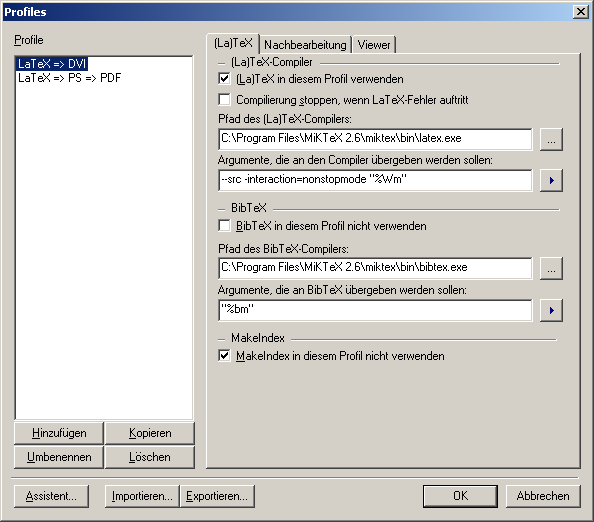
\includegraphics[width=0.49\textwidth]{techniccenter-profile-dvi-26} &
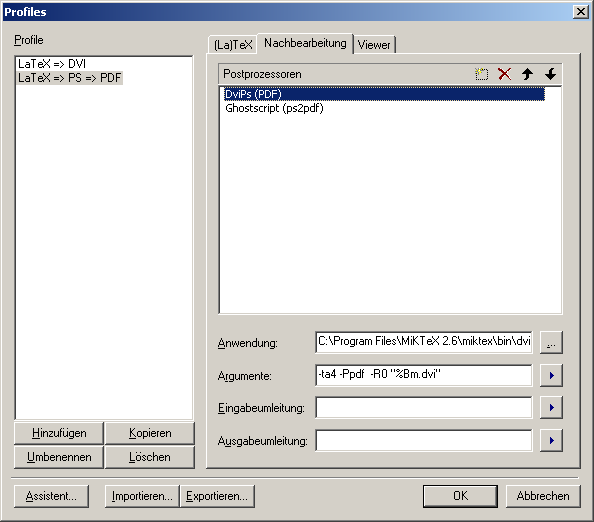
\includegraphics[width=0.49\textwidth]{techniccenter-profile-dvips-26} \\[4pt]
(a) & (b)
\end{tabular}
\caption{Spezifikation der Ausgabeprofile in TeXnicCenter.}
\label{fig:techniccenter-profile-latex}
\end{figure}

Für diese Vorlage wird die verwendung des Ausgabeprofiels \texttt{LaTeX => PDF} empfohlen.

%
%In der Datei \verb!tc_output_profiles_sumatra.tco! sind  folgende beiden "`maßgeschneiderten"' Ausgabeprofile für TexNicCenter angelegt (Import über \textsf{Build} $\rightarrow$ \textsf{Define Output Profiles ...}):
%\begin{itemize}
	%\item \verb!LaTeX => PDF (Sumatra)! -- Standard, direkte Erzeugung von PDF,
	%\item \verb!LaTeX => PS => PDF (Sumatra)! -- PDF "`klassisch"' via DVI und PS.
%\end{itemize}
%
%
%
%\subsubsection{Profil "`\texttt{LaTeX => PDF (Sumatra)}"'}
%
%Das ist das mit diesem Setup normalerweise verwendete Standardprofil.
%
%\paragraph{(La)Tex:}
%\begin{itemize}
  %\item Path to the (La)TeX compiler: \\
        %\begin{small} \verb!C:\Program Files\MiKTeX 2.8\miktex\bin\pdflatex.exe!\end{small}
  %\item Command line arguments to pass to the compiler:\\
%\begin{small}
   %\verb!-synctex=-1 -interaction=nonstopmode "%pm"!
%\end{small}
%\end{itemize}
%
%\paragraph{Postprocessor:} 
%leer, kein Postprocessor notwenig.
%
%\paragraph{Viewer:}
%\begin{itemize}
%\item Path of executable: \\
%\begin{small}
    %\verb!C:\Program Files\SumatraPDF\SumatraPDF.exe ! \\ 
    %\verb!-inverse-search "\"C:\Program Files\TeXnicCenter\TEXCNTR.EXE\" !\\
    %\verb!/ddecmd \"[goto('%f','%l')]\""!
%\end{small}
%%
%\item View project's output: \\
%\begin{small}
    %\checkbox\ Command line argument \\\
    %Command: \verb!"%bm.pdf"!
%\end{small}
%%
%\item Forward search:\\
%\begin{small}
    %\checkbox\ DDE command \\\
    %Command: \verb![ForwardSearch("%bm.pdf","%Wc",%l,0)]! \\
    %Server: \verb!SUMATRA! \\
    %Topic: \verb!Control!
%\end{small}
%\item Close document before running (La)TeX:\\
%\begin{small}
    %\checkbox\ Do not close
%\end{small}
%\end{itemize}
%
%
%
%
%\subsubsection{Profil "`\texttt{LaTeX => PS => PDF (Sumatra)}"'}
%
%Profil ausschließlich für den DVI-PS-Workflow (über DVI und PostScript).
%
%\paragraph{(La)Tex:}
%\begin{itemize}
  %\item Path to the (La)TeX compiler: \\
        %\begin{small} \verb!C:\Program Files\MiKTeX 2.8\miktex\bin\latex.exe!\end{small}
  %\item Command line arguments to pass to the compiler:\\
%\begin{small}
   %\verb!-synctex=-1 -interaction=nonstopmode "%pm"!
%\end{small}
%\end{itemize}
%
%\paragraph{Postprocessor:}
%\begin{itemize}
  %\item DviPS (PDF): \\
        %\begin{small} 
        %Executable: \verb!C:\Program Files\MiKTeX 2.8\miktex\bin\dvips.exe! \\
        %Arguments: \verb!-ta4 -P pdf -R0 "%Bm.dvi"!
        %\end{small}
  %\item Ghostscript (ps2pdf):\\
  		%\begin{small} 
        %Executable: \verb!C:\Program Files\gs\gs8.64\bin\gswin32c.exe! \\
        %Arguments: \verb!-q -dPDFSETTINGS=/prepress -sPAPERSIZE=a4 -dSAFER! \\
         %\verb!-dBATCH -dNOPAUSE -sDEVICE=pdfwrite -sOutputFile="%bm.pdf"! \\
         %\verb!-c save pop -f "%bm.ps"!
      %\end{small}
%\end{itemize}
%
%\paragraph{Viewer:}
%wie in Profil A. (\texttt{LaTeX => PDF (Sumatra)}).
	% Technische Ergänzungen
%\chapter{Abläufe}

\section{Hauptmenu}
\begin{figure}[htbp]
	\centering
	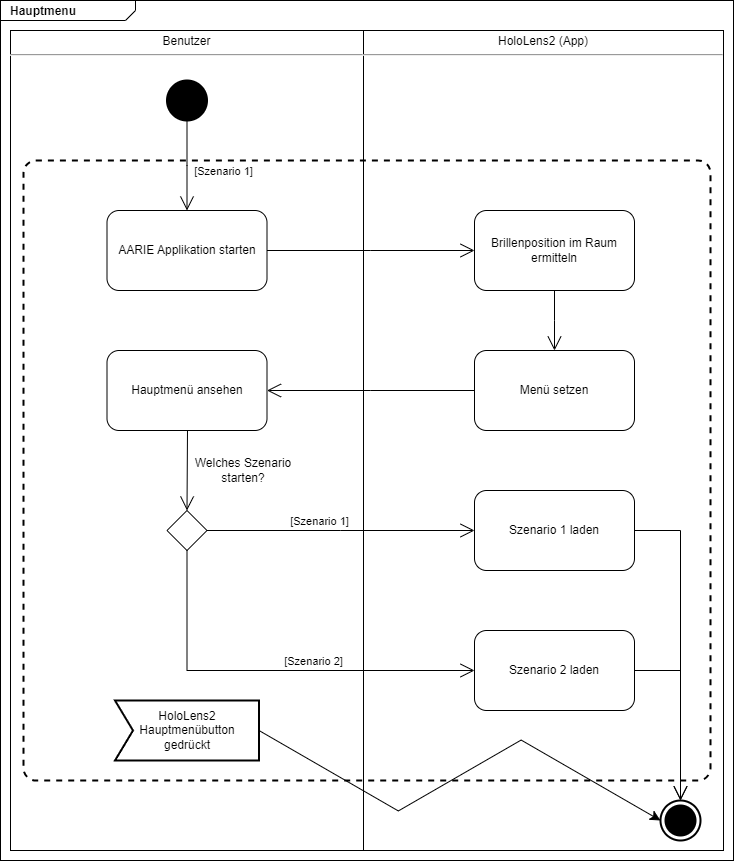
\includegraphics[width=0.80\textwidth]{images/Hauptmenu_Ablauf}
	\caption{Hauptmenu UML Aktivitätsdiagramm}
\end{figure}
\newpage

\section{Nachrichtenaustausch Anwendungsszenario}
\begin{figure}[htbp]
	\centering
	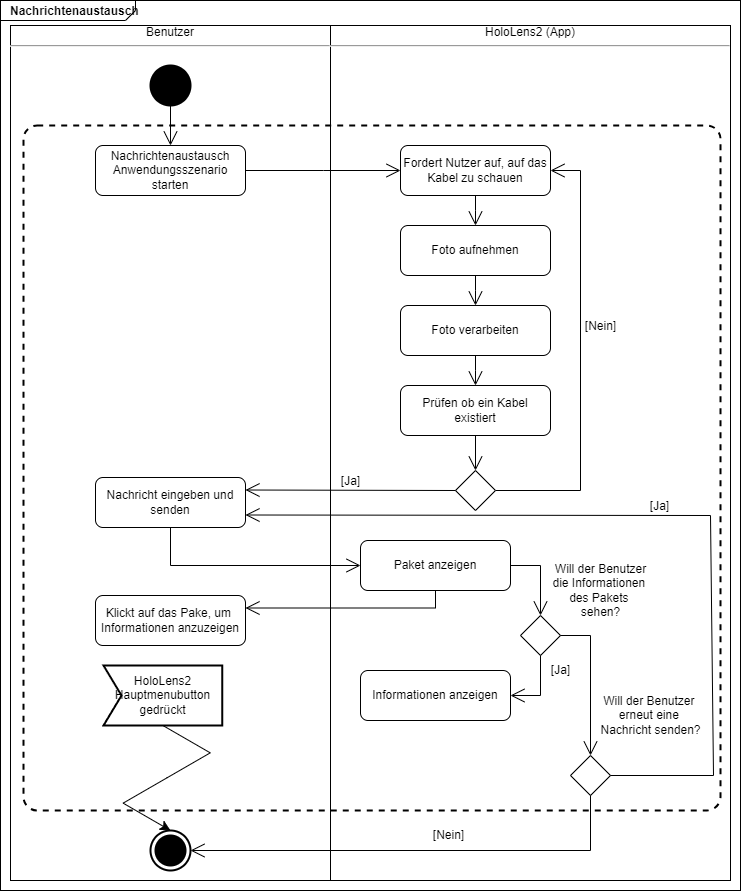
\includegraphics[width=\textwidth]{Nachrichtenaustausch_Ablauf.png}
	\caption{Nachrichtenaustausch UML Aktivitätsdiagramm}
\end{figure}
\newpage

\section{Knapsack-Problem Anwendungsszenario}
\begin{figure}[htbp]
	\centering
	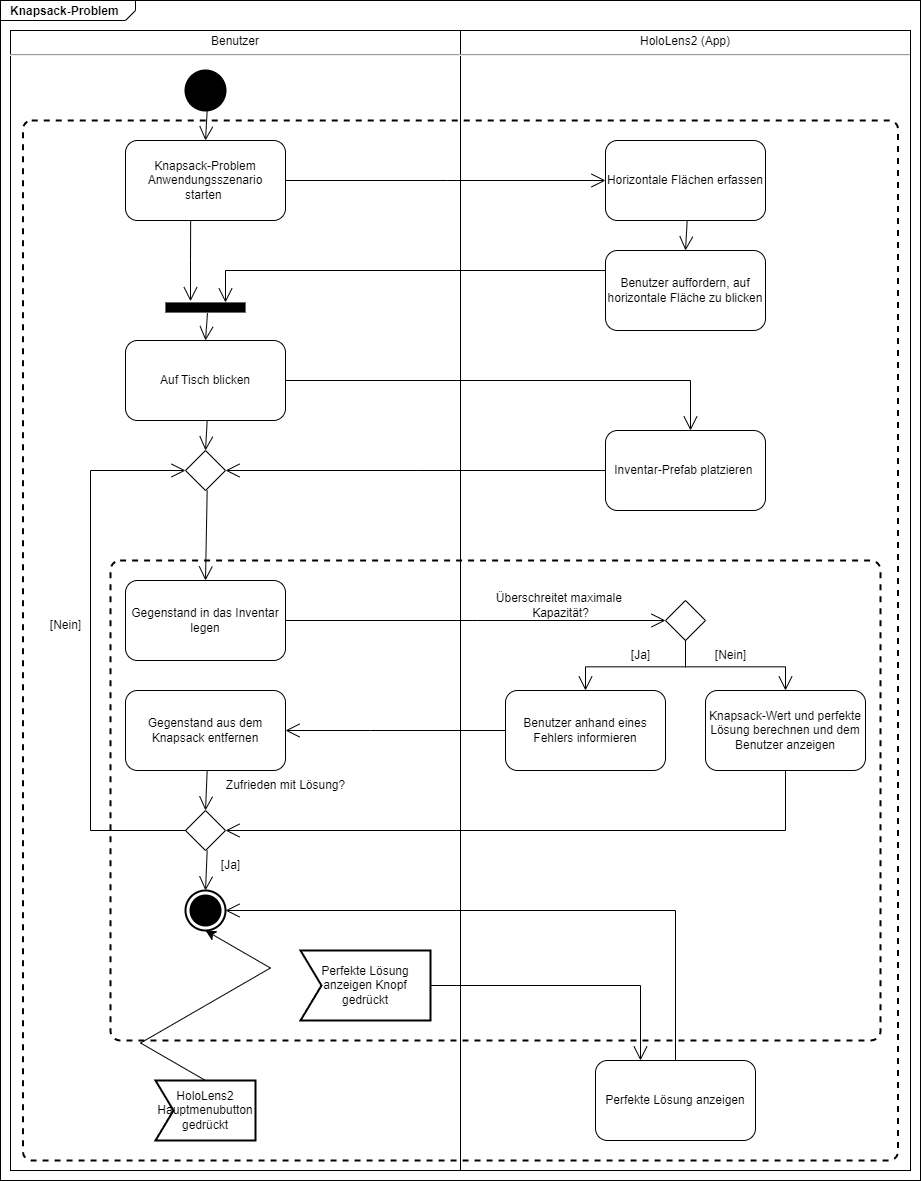
\includegraphics[width=\textwidth]{images/Knapsack_Ablauf.png}
	\caption{Knapsack-Problem UML Aktivitätsdiagramm}
\end{figure}
\newpage	% Inhalt der CD-ROM/DVD
%\chapter{Chronologische Liste der Änderungen}

\begin{sloppypar}
\begin{description}

\item[2018/07/02]
Überarbeitung für das Schuljahr 2018/19
\begin{itemize}
  \item Indixierung der Literatur nach Titel und Autor
  \item Allgemeiner Index für eigene Begriffe
  \item Software überarbeitet und auf den neuesten Stand gebracht
  \item Umstieg von biblatex auf biber
  \item Subfigure hinzugefügt
  \item Settings aus \_Diplomarbeit.tex ausgelagert
\end{itemize}


\item[2017/04/03]
FAQ hinzugefügt

\item[2017/03/28]
Anpassungen an sehr lange URLs in den Fußnoten

\item[2017/03/21]
Anpassungen an sehr lange Titel und Untertitel

\item[2016/10/20]
Neues Zitierformat (footcite)

\item[2016/04/04]
Umlaute in Codelistings möglich

\item[2015/10/11]
Dokumentationsseiten aus PDF Formular

\item[2015/10/07]
Umstieg von listings2 auf listingsutf8

\item[2015/10/06]
Syntax Highlighting umschaltbar zwischen Farbe und Schwarz / Weiß

\item[2015/09/29]
Neues Deckblatt

\item[2015/09/03]
Einseitig / Zweiseitig umschaltbar 

\item[2012/08/29]
Einstellbare Seitenränder durch das geometry Package

\item[2010/11/22]
Überarbeitung der originalen Vorlagen von Dr.\ Wilhelm Burger und Anpassung an
die Bedürfnisse einer HTL-
Wichtigste Änderungen:
\begin{itemize}
  \item Wechsel auf UTF8
  \item Wechsel auf listings2-beta
  \item Neue Code-Umgebungen für Python und C\#
  \item Vorlagen für Normen und Patente im Literaturverzeichnis
  \item Hinweise auf DVI-PS Workflow entfernt
  \item Kapitel zur automatischen \latex-Code erzeugung hinzugefügt
\end{itemize}
%
\end{description}

\end{sloppypar}

%\section*{To Do} 
%\begin{itemize}
%\item Literaturempfehlungen zum Schreiben von Diplomarbeiten
%\item Hinweise für Literatursuche (Bibliotheksverbund, CiteSeer,...)
%\end{itemize}



	% Chronologische Liste der Änderungen
%\chapter{\latex-Quellkode}
\label{app:latex}

\section*{Hauptdatei {\tt\_Diplomarbeit.tex}}

\begin{footnotesize}
\verbatiminput{_Diplomarbeit.tex}
\end{footnotesize}


%\vspace*{2cm}
\hrule
\hrule

\paragraph{Anmerkung:}
Das sollte nur ein \emph{Beispiel} für die Einbindung von Quellcode
in einem Anhang sein. Der \latex-Quellkode der eigenen
Diplomarbeit ist meist \emph{nicht} interessant genug, um ihn hier
wiederzugeben!

	% Quelltext dieses Dokuments

%%%----------------------------------------------------------
%Literatur
\chapter{Literatur}

\begin{itemize}
    \item Blender. URL: \url{https://www.blender.org/about/} (besucht am 06.10.2023).
    \item Scrum Alliance Inc. WHAT IS SCRUM? URL: \url{https://www.scrumalliance.org/about-scrum#} (besucht am 06.10.2023).
    \item Scrum-Master.de Scrum-Rollen - Product Owner. URL: \url{https://scrum-master.de/Scrum-Rollen/Scrum-Rollen_Product_Owner} (besucht am 10.11.2023).
    \item Scrum-Master.de Scrum-Rollen - Scrum Master. URL: \url{https://scrum-master.de/Scrum-Rollen/Scrum-Rollen_ScrumMaster} (besucht am 10.11.2023).
    \item Scrum-Master.de Scrum-Rollen - Team. URL: \url{https://scrum-master.de/Scrum-Rollen/Scrum-Rollen_Team} (besucht am 10.11.2023).
    \item Scrum-Master.de Scrum-Meetings - Sprint - Team. URL: \url{https://scrum-master.de/Scrum-Meetings/Sprint} (besucht am 10.11.2023).
    \item Scrum-Master.de Scrum-Meetings - Sprint Planing Meeting - Team. URL: \url{https://scrum-master.de/Scrum-Meetings/Sprint_Planning_Meeting} (besucht am 10.11.2023).
    \item Scrum-Master.de Scrum-Meetings - Daily Scrum Meeting - Team. URL: \url{https://scrum-master.de/Scrum-Meetings/Sprint} (besucht am 10.11.2023).
    \item Scrum-Master.de Scrum-Meetings - Sprint Review Meeting - Team. URL: \url{https://scrum-master.de/Scrum-Meetings/Sprint_Review_Meeting} (besucht am 10.11.2023).
    \item Scrum-Master.de Scrum-Meetings - Sprint Retroperspektiv Meeting - Team. URL: \url{https://scrum-master.de/Scrum-Meetings/Sprint_Review_Meeting} (besucht am 10.11.2023).
    \item GeeksForGeeks.org Introduction to Knapsack Problem, its Types and How to solve them. URL: \url{https://www.geeksforgeeks.org/introduction-to-knapsack-problem-its-types-and-how-to-solve-them/} (besucht am 18.02.2024).
    \item Unity Dokumentation GameObjects. URL: \url{https://docs.unity3d.com/Manual/GameObjects.html} (besucht am 18.02.2024).
    \item Microsoft Dokumentation. MIXED REALITY TOOLKIT 3. URL: \url{https://learn.microsoft.com/en-us/windows/mixed-reality/mrtk-unity/mrtk3-overview/} (besucht am 05.11.2023).
    \item Khronos Group. OPENXR. URL: \url{https://www.khronos.org/openxr/} (besucht am 05.11.2023).
    \item Medium. CREATING MANAGER CLASSES IN UNITY. URL: \url{https://sneakydaggergames.medium.com/creating-manager-classes-in-unity-a77cf7edcba5} (besucht am 05.11.2023).
    \item Unity Dokumentation. AR Plane Manager. URL: \url{https://docs.unity.cn/Packages/com.unity.xr.arfoundation@4.1/manual/plane-manager.html} (besucht am 05.11.2023).
    \item Unity Dokumentation. AR Raycast Manager. URL: \url{https://docs.unity.cn/Packages/com.unity.xr.arfoundation@5.0/api/UnityEngine.XR.ARFoundation.ARRaycastManager.html} (besucht am 05.11.2023).
    \item Unity Dokumentation. Plane. URL: \url{https://docs.unity3d.com/ScriptReference/Plane.html} (besucht am 13.12.2023).
    \item Unity Dokumentation. Scenes. URL: \url{https://docs.unity3d.com/Manual/CreatingScenes.html} (besucht am 13.12.2023).
    \item Unity Dokumentation. Prefabs. URL: \url{https://docs.unity3d.com/Manual/Prefabs.html} (besucht am 15.01.2024).
    \item Unity Dokumentation. Bounds. URL: \url{https://docs.unity3d.com/ScriptReference/Bounds.html} (besucht am 16.01.2024).
    \item Unity Dokumentation. Renderer. URL: \url{https://docs.unity3d.com/ScriptReference/Renderer.html} (besucht am 16.01.2024).
    \item Color Doku, URL:  \url{https://docs.unity3d.com/ScriptReference/Color.html%7D} besucht am 4.11.2023).
    \item Trackable Doku, URL:  \url{https://docs.unity3d.com/2019.2/Documentation/ScriptReference/Experimental.XR.TrackableType.html%7D} (besucht am 18.11.2023).
    \item ARRaycastHit Doku, URL:  \url{https://docs.unity3d.com/Packages/com.unity.xr.arfoundation@4.0/api/UnityEngine.XR.ARFoundation.ARRaycastHit.html%7D} (besucht am 18.11.2023).
    \item PhotoCaputre, URL:  \url{https://docs.unity3d.com/ScriptReference/Windows.WebCam.PhotoCapture.html%7D} (besucht am 2.11.2023).
    \item Unity. TextMeshPro. URL: \url{https://docs.unity3d.com/Manual/com.unity.textmeshpro.html} (besucht am 15.12.2023).
    \item Foto-/Videokamera in Unity, URL:  \url{https://learn.microsoft.com/de-de/windows/mixed-reality/develop/unity/locatable-camera-in-unity%7D} (besucht am 2.11.2023)
    \item Microsoft. Buttons — MRTK2. URL: \url{https://learn.microsoft.com/en-us/windows/mixed-reality/mrtk-unity/mrtk2/features/ux-building-blocks/button?view=mrtkunity-2022-05} (besucht am 7.11.2023).
    \item Microsoft. Menü Nahe — MRTK2. URL: \url{https://learn.microsoft.com/de-de/windows/mixed-reality/mrtk-unity/mrtk2/features/ux-building-blocks/near-menu?view=mrtkunity-2022-05} (besucht am 8.11.2023).
    \item Unity. Load scene on button press. URL: \url{https://blog.insane.engineer/post/unity_button_load_scene/} (besucht am 8.11.2023).
    \item Blender. Can't see added cube on my scene collection [duplicate]. URL: \url{https://blender.stackexchange.com/questions/162424/cant-see-added-cube-on-my-scene-collection} (besucht am 15.11.2023).
    \item Blender. How do I Inset a face equally? URL: \url{https://blender.stackexchange.com/questions/50876/how-do-i-inset-a-face-equally} (besucht am 17.11.2023).
    \item Blender. Modifier. URL: \url{https://docs.blender.org/manual/en/latest/modeling/modifiers/index.html} (besucht am 10.12.2023).
    \item Blender. Object Modes. URL: \url{https://docs.blender.org/manual/en/latest/editors/3dview/modes.html} (besucht am 21.12.2023).
    \item Blender. Loop Tools. URL: \url{https://docs.blender.org/manual/en/latest/addons/mesh/looptools.html} (besucht am 20.11.2023).
    \item Blender. Vertices. URL: \url{https://docs.blender.org/manual/en/latest/scene_layout/object/properties/instancing/verts.html} (besucht am 05.01.2024).
    \item Blender. Meshes. URL: \url{https://docs.blender.org/manual/en/latest/modeling/meshes/index.html} (besucht am 10.11.23).
    \item Blender. Array-Modifier. URL: \url{https://docs.blender.org/manual/en/latest/modeling/modifiers/generate/array.html} (besucht am 11.01.2024)
    \item Blender. Extrude. URL: \url{https://docs.blender.org/manual/de/dev/grease_pencil/modes/edit/point_menu.html#extrude} (besucht am 20.2.2024)
    \item Autodesk FBX. Getting started. URL: \url{https://help.autodesk.com/view/FBX/2020/ENU/?guid=FBX_Developer_Help_welcome_to_the_fbx_sdk_html} (besucht am 07.01.2024).
    \item Autodesk FBX. URL: \url{https://www.autodesk.com/products/fbx/overview} (besucht am 07.01.2024).
    \item Blender. Images as Planes. URL: \url{https://docs.blender.org/manual/en/latest/addons/import_export/images_as_planes.html} (besucht am 05.12.2024).
    \item Mozilla Developer Network. HTML. URL: \url{https://developer.mozilla.org/en-US/docs/Web/HTML} (besucht am 19.02.2024).
    \item Mozilla Developer Network. CSS. URL: \url{https://developer.mozilla.org/en-US/docs/Web/CSS} (besucht am 19.02.2024).
    \item Mozilla Developer Network. JavaScript. URL: \url{https://developer.mozilla.org/en-US/docs/Web/JavaScript} (besucht am 19.02.2024).
    \item Bootstrap Dokumentation. URL: \url{https://getbootstrap.com/docs/5.1/getting-started/introduction/} (besucht am 20.02.2024).
    \item Bootstrap Dokumentation. CDN-Links. URL: \url{https://getbootstrap.com/docs/5.2/getting-started/introduction/} (besucht am 20.02.2024).
    \item Unity. QR-Code Tracking. URL: \url{https://learn.microsoft.com/en-us/samples/microsoft/mixedreality-qrcode-sample/qr-code-tracking-in-unity/} (besucht am 2.11.2023).
    \item Unity. QR-Code Tracking Overview. URL: \url{https://learn.microsoft.com/de-de/windows/mixed-reality/develop/advanced-concepts/qr-code-tracking-overview} (besucht am 30.10.2023).
    \item Unity. SpacialGraphNode Class. URL: \url{https://learn.microsoft.com/de-de/dotnet/api/microsoft.mixedreality.openxr.spatialgraphnode?view=mixedreality-openxr-plugin-1.9} (besucht am 2.11.2023).
    \item Scholl, Armin. \textit{Die Befragung} 3. Aufl. Stuttgart: utb GmbH, 2014.
    \item Mayer, Horst. \textit{Interview und schriftliche Befragung. Entwicklung, Durchführung und Auswertung} 3. Aufl. München: R. Oldenbourg, 2008.
    \item Bühner, Markus. \textit{Einführung in die Test- und Fragebogenkonstruktion.} 3. Aufl. München: Pearson Studium, 2021.
    \item Unity. GameObjects. URL: \url {https://docs.unity3d.com/Manual/GameObjects.html} (besucht am 15.12.2023).
    \item Unity. Texture2D. URL: \url {https://docs.unity3d.com/ScriptReference/Texture2D.html} (besucht am 15.12.2023).
    \item Unity. Canvas. URL: \url{https://docs.unity3d.com/Packages/com.unity.ugui@1.0/manual/UICanvas.html} (besucht am 21.02.2024)
    \item Unity. Job system overview. URL: \url{https://docs.unity3d.com/Manual/JobSystemOverview.htmll} (besucht am 21.02.2024)
    \item Unity. PhotoCapture. URL: \url{https://docs.unity3d.com/Manual/JobSystemOverview.htmll} (besucht am 22.02.2024)
\end{itemize}

% Add the rest of your document content below.



%Ausgabe der automatischen Zusatzdaten: Glossar, Index, Literaturverzeichnis
\clearpage
\printglossaries

\clearpage
%\chapter*{Index}
\addcontentsline{toc}{chapter}{Index}
\printindex[allgemein]

\printindex

\printindex[name]

\printindex[title]


%Literaturverzeichnis
\clearpage
\addcontentsline{toc}{chapter}{\bibname}

\printbibliography


%%%----------------------------------------------------------

%%%Messbox zur Druckkontrolle
%\chapter*{Messbox zur Druckkontrolle}



\begin{center}
{\Large --- Druckgröße kontrollieren! ---}

\bigskip

\Messbox{100}{50} % Angabe der Breite/Hoehe in mm

\bigskip

{\Large --- Diese Seite nach dem Druck entfernen! ---}

\end{center}



\end{document}
